% !TeX document-id = {beb7ced9-b3cd-42b2-b16a-3ed3c633a1d9}
\documentclass[]             % options: RDPonly, coveronly, nocover
{NASA}                       %   plus standard article class options
%\DeclareRobustCommand{\mmodels}{\mathrel{|}\joinrel\Relbar}

\usepackage[utf8]{inputenc}
\usepackage{csquotes}
\usepackage{setspace}
\usepackage{hyperref}
\usepackage{amsmath, amssymb, amscd, amsthm, amsfonts}
\usepackage{mathtools}
\usepackage{graphicx}
\usepackage{hyperref}
\usepackage{amsthm}
\usepackage[english]{babel}
\usepackage{stmaryrd}
\usepackage{proof}
\usepackage{tikz-cd}
\tikzcdset{scale cd/.style={every label/.append style={scale=#1},
    cells={nodes={scale=#1}}}}
% Added for subfigures
\usepackage{caption}
\usepackage{subcaption}
\usepackage{afterpage}

\newtheorem{theorem}{Theorem}[section]
\newtheorem{corollary}{Corollary}[theorem]
\newtheorem{lemma}[theorem]{Lemma}
\newtheorem{example}{Example}
\theoremstyle{definition}
\newtheorem{definition}{Definition}[section]

\newcommand{\B}{\mathbf{B}}
\newcommand{\w}{\mathbf{w}}
\newcommand{\citationneeded}{\footnote{\textbf{CITATION NEEDED}}}

% Globally redefine pgfpicture to use \Large fonts
\let\origpgfpicture=\pgfpicture
\def\pgfpicture{\origpgfpicture\Large}

% Try loading this package to prevent so much hyphenation
% as recommended by https://stackoverflow.com/questions/1609837/latex-breaking-up-too-many-words
\usepackage{microtype}

% Try setting matrix columns closer
\setlength\arraycolsep{2pt}

\title{A Survey of Distributed Systems Challenges for Wildland
  Firefighting and Disaster Response}

\author{Lawrence Dunn and Alwyn E. Goodloe}

\AuthorAffiliation{Lawrence Dunn \\ Department of Computer and Information
  Science \\ University of Pennsylvania \\ Philadelphia, PA \\ Alwyn Goodloe\\                                          % for cover page
  NASA Langley Research Center, Hampton, Virginia
}
\NasaCenter{Langley Research Center\\Hampton, Virginia 23681-2199}
\Type{TM}                    % TM, TP, CR, CP, SP, TT
\SubjectCategory{64}         % two digit number
\LNumber{XXXXX}              % Langley L-number
\Number{XXXXXX}              % Report number
\Month{12}                   % two digit number
\Year{2022}                  % four digit number
\SubjectTerms{Distributed Systems, Formal Methods, Logic, }     % 4-5 comma separated words
\Pages{46}                   % all the pages from the front to back covers
\DatesCovered{}              % 10/2000--9/2002
\ContractNumber{}            % NAS1-12345
\GrantNumber{}               % NAG1-1234
\ProgramElementNumber{}
\ProjectNumber{}             % NCC1-123
\TaskNumber{}                % Task 123
\WorkUnitNumber{}            % 123-45-67-89
\SupplementaryNotes{}
\Acknowledgment{The work was conducted during a summer internship at the NASA Langley Research Center in the Safety-Critical Avionics Systems Branch focusing on distributed computing  issues arising in the Safety Demonstrator challenge in the NASA Aeronautics System Wide Safety (SWS) program.}

%Added for Pandoc
\providecommand{\tightlist}{%
  \setlength{\itemsep}{0pt}\setlength{\parskip}{0pt}}


\abstract{The System Wide Safety (SWS) program has been investigating
  how crewed and uncrewed aircraft can safely operate in shared
  airspace. Enforcing safety requirements for distributed agents
  requires coordination by passing messages over a communication
  network. Unfortunately, the operational environment will not admit
  reliable high-bandwidth communication between all agents,
  introducing theoretical and practical obstructions to global
  consistency that make it more difficult to maintain safety-related
  invariants. Taking disaster response scenarios, particularly
  wildfire suppression, as a motivating use case, this self-contained
  memo discusses some of the distributed systems challenges involved
  in system-wide safety through a pragmatic lens. We survey topics
  ranging from consistency models and network architectures to data
  replication and data fusion, in each case focusing on the practical
  relevance of topics in the literature to the sorts of scenarios and
  challenges we expect from our use case.  }

\begin{document}
\newpage
\setcounter{tocdepth}{2}
\tableofcontents
\newpage

\section{Introduction}\label{introduction}

Civil aviation has traditionally focused primarily on the efficient
and safe transportation of people and goods via the airspace. Despite
the inherent risks, the application of sound engineering practices and
conservative operating procedures has made flying the safest mode of
transport today. Now the desire not to compromise this safety makes it
difficult to integrate unmanned vehicles into the airspace, accomodate
emerging applications, and keep pace with unprecedented recent growth
in commercial aviation. To that end, the System Wide Safety (SWS)
project of the NASA Aeronautics' Airspace Operations and Safety
Program (AOSP) has been investigating technologies and methods by
which crewed and uncrewed aircraft may safely operate in shared
airspace.

This memo surveys topics in computing that are relevant to maintaining
system-wide safety across large, physically distributed data and
communication systems. It aims to be self-contained and accessible to
a technical audience without a deep background in distributed
systems. Our primary motivating use cases have been taken from civil
emergency response scenarios, especially wildfire suppression and
hurricane relief, primarily for three reasons. First, improved
technology for wildfire suppression, especially related to
communications and data sharing, is frequently cited as a national
priority \cite{pcast2023}.  Second, the rules for operating in the US
national airspace are typically relaxed during natural disasters and
relief efforts, so this is a suitable setting for testing new
technologies. Finally, this setting is an excellent microcosm for the
sorts of general challenges faced by other, non-emergency
applications.

If there is a central theme uniting the sections of this manuscript,
it is \emph{continuity} in the sense considered by
topology.\footnote{For a typical introductory textbook see
\cite{mendelson2012introduction}.} The systems we consider will be
subject to harsh operating conditions that limit how well they can
perform---for example, wireless communication is typically less
reliable during inclement weather. To build a system that is
predictable (clearly a prerequisite for safety), one must ensure the
system is flexible enough to perform reasonably well under a wide
variety of adverse conditions. In other words, the behavior of a safe
system should in some sense be a \emph{continuous} function of its
inputs and environment. This sort of robust design is particularly
challenging because distributed systems designers are forced to make
delicate tradeoffs between competing objectives, most famously between
performance and consistency, the topic of Section
\ref{sec:background}.

\subsection{Summaries of the sections}\label{summaries-of-the-sections}

Sections \ref{sec:disaster-response}--\ref{sec:desiderata} contain
background material on disaster response, distributed systems, and the
specifics of our use case. The critical takeaway of these sections is
that system-wide safety is, at least in part, a computer science
problem, indeed a software problem, and not ``just'' a matter of
engineering better hardware. Sections
\ref{sec:networking}--\ref{sec:data-fusion} survey particular topics
from the distributed systems literature, proceeding from lower-level
considerations to higher-level ones; these sections may be read
independently of each other. Below we summarize each section.

Section \ref{sec:disaster-response} starts with a pragmatic summary of
disaster response and some of the relevant computing challenges in
that setting. We aim to justify and explain the role of distributed
systems theory in system-wide safety by citing real examples
encountered in disaster response scenarios.

Section \ref{sec:background} is an introduction to distributed
systems, culminating in a illustrative result: the ``CAP'' theorem(s)
for the atomic and sequential consistency models (Theorems
\ref{thm:cap} and \ref{thm:cap-sequential}, respectively). CAP is
considered a ``negative'' result, meaning it proves something cannot
be done. The CAP theorem proves that strong consistency for a
distributed system makes systemwide network performance an upper bound
on the availability of a system to do useful work for clients, which
for our purposes is an unacceptable restriction. The practical
significance of CAP is that in emergency response environments, agents
will always act with incomplete information about the global system, a
key motivation for Section \ref{sec:continuous-consistency}.

Section \ref{sec:desiderata} refines our assumptions and identifies
desirable properties of systems for our use case. We use these points to
frame the discussion of systems and protocols in subsequent sections.

Section \ref{sec:networking} examines networking considerations. Our
vision of future emergency communication networks integrates concepts
from delay/disruption-tolerant networks (DTN) and mobile ad-hoc
networks (MANET) to provide digital communications that are robust to
a turbulent operational environment. We also examine the state of
software-defined networking (SDN). SDN is an emerging field that puts
networking protocols on the same footing as ordinary computer
programs. In theory, this should furnish computer networking with all
the benefits of modern software engineering, such as reprogrammable
hardware, rapid iteration, version control, and especially formal
verification.

Section \ref{sec:continuous-consistency} describes a hypothetical
application that might be used in a disruption-heavy network: a data
replication service built on Yu and Vahdat's theory of ``conits"
(short for ``consistency unit'') \cite{2002tact}. This framework
realizes a \emph{continuous} consistency model in the sense that, as
typically configured, it provides neither strong consistency nor
guaranteed high-availability, but rather a quantifiable and
controllable tradeoff between the two. The key idea is that many
applications can tolerate inconsistency among replicas of a data item
if an upper bound on the divergence between replicas is enforced. A
conit-based database replication framework would allow system
designers to define units of replicated data whose consistency is of
interest, enforce policies bounding inconsistency between replicas of
these items, and even dynamically tune these policies on the fly. We
believe that only a conit-based replication infrastructure can provide
the strict guarantees required for safety-related systems while also
tolerating the adverse environments and real-world limitations of the
systems we have in mind.

Section \ref{sec:data-fusion} concerns data fusion. Now and in the
future, agents in disaster scenarios will make decisions informed by
many different kinds of information. Efficient integration,
processing, filtering, and dissemination of this information will be
necessary to avoid ``swimming in sensors and drowning in data''
\cite{2010:magnuson}.  This task is especially challenging because
agents will often work with incomplete or out of date information, and
different sources of the same data may be contradictory, e.g. first
responders may receive contradictory reports about whether a structure
is occupied. One promising trend in this space, which we briefly
introduce in this section, is the development of sheaf theory as a
natural mathematical model for data fusion
\cite{2017robinsonCanonical}. Sheaf theory provides a rigorous
framework for discussing how heterogeneous sources of noisy data can
be integrated into a coherent picture, and can formally measure how
well this task has been achieved.

We conclude in Section \ref{sec:conclusion} by recapping some of the
main themes in this document and highlighting areas where design
decisions at various levels must be made to build a system that is
tuned to the exact conditions we can expect from real-world
scenarios. Such decisions might be informed by a combination of
simulation and experimentation in the field.

\section{Coordination Challenges in Disaster Response}
\label{sec:disaster-response}

This section explains aspects of disaster response (particularly
firefighting) scenarios that motivate the remainder of this
document. We describe how real-world environments give rise to
foundational challenges that must be addressed through the application
of distributed computing principles. Even deploying the best
communications equipment cannot realistically avoid the fundamental
computer scientific problems raised when many distributed agents try
to coordinate their actions over a widespread area.

The operational environment of wildfire suppression, hurricane relief,
and other disaster settings is generally characterized by systemic
communications challenges. It is not surprising that a 2023 report on
wildland firefighting modernization by the President’s Council of
Advisors on Science and Technology (PCAST) cites ``the vulnerabilities
and shortfalls in wildland firefighter communications, connectivity,
and technology interoperability'' in their first of five
recommendations \cite{pcast2023}. These shortfalls can be partly
attributed to factors that are simply inherent to disaster response:
remote locations, difficult terrain, damaged infrastructure, harsh
weather, and limited battery power, to name a few.

Agents in the field generally experience high packet loss (when
considering digital communication), garbled transmissions, and
unpredictable latencies when passing information over the
communication network(s). A conservative view suggests expecting the
worst performance at particularly inopportune times, simply because
the conditions that prompt urgent communication can be expected to
correlate with those that make communication difficult. One
possibility is that the disaster itself damages the communications
infrastructure.  Another example, which is true tautologically, is
that a communications network is the most congested, and therefore the
least available, precisely when everyone needs to use it. Both of
these phenomena were famously exhibited in the immediate aftermath of
the September $11^\textrm{th}$ terrorist attacks when sudden user
demand and severed trunk cables brought New York public cell phone
networks virtually to a halt \cite{2011:Reardon}. Other networks along
the East Coast, as well as dedicated networks for first responders,
experienced similar effects.

From a systems perspective, an unreliable network presents a challenge
for coordinating distributed agents. A root cause of this problem is
that coordinated action requires some notion of consistency,
i.e.~agreement, among data shared between agents. We shall make this
somewhat vague notion more precise in Section \ref{sec:background},
but a simple example is that it is very important for everyone to
agree which firetrucks have been dispatched to which scenes, which
tasks should be prioritized, or which radios have been reserved from
the {\mbox{NIICD}} radio cache \cite{radiocache} and for whom. The
exact meaning of ``consistency'' varies between applications, but a
general observation is that stronger standards for consistency are
more difficult to maintain than relaxed ones because they require
exchanging more information with other agents quickly, putting a
heavier burden on the network. When the network is slow, system
components that need to communicate may have to wait for network to
deliver their messages, diminishing the efficacy and coherence of the
system.

\subsection{Communication and Safety}
\label{communication-and-safety}

Many complications in the field are exacerbated by a poor
communications environment. In this setting, agents must choose
between long delays in sending and receiving information or acting
with only limited knowledge. Typically they will experience some
amount of both. Both options present safety challenges because
operational safety, by nature, requires agents to gather information
about their environment and react to it quickly and systematically. In
other words, both inaction and uninformed action are problems. This
turns out to be deeply related to a computer science phenomenon
generally known as the safety/liveness tradeoff.

As a running example, we consider the use of firefighting airtankers,
the largest of which are the Very Large Airtankers (VLATs), defined as
those carrying more than 8,000 gallons of water or fire retardant
\cite{2019:airtankerops}. The largest VLATs can carry more than 20,000
gallons, weighing about 170,000 pounds. This weight is typically
dropped from a mere 250 feet above the tree canopy
\cite{2019:airtankerops}, though the complexity of the maneuver means
errant drops are sometimes performed even lower than this, easily
crushing a ground vehicle \cite{2019:stickney}. A 2018 accident led to
the death of one firefighter and the injury of three others when an
87-foot Douglas Fir tree was knocked down by an unexpectedly forceful
drop from a Boeing 747-400 Supertanker \cite{2018:calfire}.

\begin{figure}[h]
  \label{fig:airtanker}
  \centering
  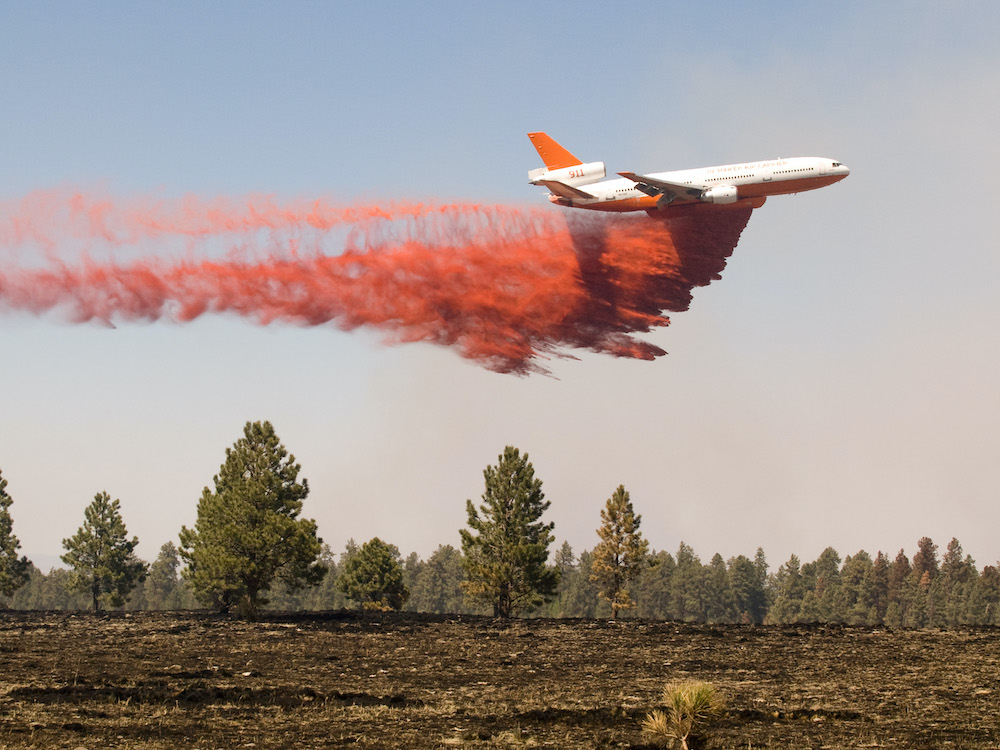
\includegraphics[scale=0.4]{images/dc10.jpg}
  \caption{A DC-10 airtanker, rated for 9,400 gallons, drops retardant above Greer, Arizona. \textbf{CITATION NEEDED}}
\end{figure}

Suppose that in the future, firefighters are equipped with GPS sensors
and digital transmitters---this could be an application running on
their personal cell phones, or better yet something running on
dedicated and more reliable equipment. A seemingly reasonable policy
would be to prohibit VLATs from performing a drop if its computers do
not have up-to-date information about the location of firefighters on
the ground. The problem is that obtaining this information may be
difficult or impossible: perhaps heavy smoke, a damaged radio tower,
or a tall ridge prevents communications between the air and ground. In
these scenarios, rigid enforcement of the safety policy would prevent
airtankers from operating.

This scenario exemplifies a classic tradeoff between opposing goals:
system \emph{safety} and system \emph{availability} (or
\emph{liveness}), elaborated on in Section \ref{sec:background}. In
the distributed computing context, safety properties guarantee that a
system will not perform an action that violates a constraint. In this
example, a reasonable safety property could look like the following:
\begin{quote}
  \interlinepenalty=10000 % Punish pagebreaks inside this quote!
  $\textbf{P}_\textrm{safe}$: All ground agents are known to be at
  least 100 feet outside the drop zone, and this information is
  current to within 30 seconds, or airtankers will not perform a drop.
\end{quote}
By contrast, liveness properties stipulate that the system
will certainly perform requested actions, typically within some time
bound. In our scenario, an expected liveness property might be the
following:
\begin{quote}
  $\textbf{P}_\textrm{live}$: Airtankers will perform a drop within 20
  minutes\footnote{In an interview with PBS, the Chief of Flight
  Operations for Cal Fire cited 20 \mbox{minutes} as the response time
  for aerial firefighting units within designated responsibility areas
  \cite{2021:aerialfirefighting}.} of receiving a request.
\end{quote}

Safety and liveness are frequently dual mandates: safety, in the sense
used here, requires a system \textbf{never} to perform certain
actions, while liveness requires a system to \textbf{always} perform
certain actions. The tension between these ideals means the two often
cannot be guaranteed simultaneously. Such is the case in our example:
if firefighters are unable to broadcast their locations to the pilot,
then the pilot's actions are impeded to maintain
\(\textbf{P}_\textrm{safe}\) at the cost of
\(\textbf{P}_\textrm{live}\), allowing the fire to spread in the
meantime.\footnote{A slight linguistic idiosyncrasy exhibited here is
that liveness properties---not just ``safety'' properties---can also
be relevant to human safety. Thus, the narrow technical meaning of
safety properties for distributed systems does not capture the whole
meaning of System Wide Safety.}

Besides the safety/liveness tradeoff, the previous example exhibits
two other aspects of reasoning about distributed systems. We pause to
draw attention to them.

\paragraph{Epistemology}
Observe that the issue in the VLAT example does not simply disappear
if no ground personnel are actually within 100 feet of a drop
zone. That is, it is not simply a matter of whether a danger is
factually present. To guarantee \(\textbf{P}_\textrm{safe}\), an
airtanker's actions must be restricted when its computers do not
\emph{know} whether an action would violate
\(\textbf{P}_\textrm{safe}\)---knowledge of the fact, and not merely
the fact of it, is the crucial part. In philosophical terms, the logic
of distributed agents is inherently an \emph{epistemic} one, meaning
it must take into account not just what is true but what is known. The
need to share knowledge is what drives communication and puts a burden
on the network.

\paragraph{Discontinuity}
The properties $\mathbf{P}_\textrm{safe}$ and
$\mathbf{P}_\textrm{live}$ are inflexible, all-or-nothing
propositions. The complexity of the operational environment demands
considering more flexible kinds of properties. Suppose that agents are
known to be $500$ feet outside the drop zone, the extra margin meaning
they are well away from any danger, but the information is only
current to within 35 seconds. Clearly this is good enough information
to authorize a drop, but strictly speaking the 5-second difference is
a violation of $\mathbf{P}_\textrm{safe}$. When safety properties are
this rigid, the system's behavior becomes overly sensitive to the
particulars of the environment and therefore difficult to predict,
which is precisely the kind of \emph{discontinuity} that we aim to
prevent. Our goal is to build reliable systems that perform well in a
wide range of circumstances.



%To make the example more extreme, $\mathbf{P}_\textrm{safe}$ is
%violated even if the information is current to within 31 seconds, so
%a mere extra second of delay makes all the difference between whether
%the VLAT can operate, even though the firefighters in question are
%clearly far outside the drop zone.



%as it makes the system's behavior difficult to predict, being so
%sensitive to the particulars of the environment. Preventing this kind
%of discontinuity can be difficult because we still want to provide
%rigorous guarantees about the system's behavior, i.e. we cannot forgo
%enforcing properties like $\mathbf{P}_\textrm{safe}$ altogether.

%In reality, a human controller would likely decide that
%the computer \emph{does} have enough information, and decide to
%override the policy. However, it is difficult to make assurances about
%a system if external actors are frequently in the habit of overruling
%its decisions.

\subsection{Communication Patterns in the Field}
\label{communication-in-practice}

We now consider some of the communication patterns that occur in
wildland firefighting. The layman reader may be surprised to learn
that the state of the art is somewhat primitive, which is partly
attributable to the fact that very little permanent infrastructure
exists in this setting. This fact is also what makes wildfires an
interesting and generalizable example for other kinds of civil
disaster environments.

One trend we will draw attention to is a kind of ``geospatial locality
of reference'' principle that system designers should take into
account. By this, we mean the happy coincidence of two observations
which, if not exactly guaranteed rules, are at least approximately
true in many circumstances. The first observation is simple:
\begin{quote}
  $\textbf{O}_1$: Agents with the most urgent need to
  coordinate their actions will tend to be located closer to each
  other and require the same kinds of information.
\end{quote}
The second observation is as follows:
\begin{quote}
  $\textbf{O}_2$: Agents that are located closer together
  will tend to have more reliable communications between them than
  agents that are far apart. Conversely, information that must travel
  a long distance tends to be delayed or degrade in quality.
\end{quote}

We will refer to the concomitance of these two facts as simply the
``locality'' principle. The reason the locality principle is crucial
is that, as we see in Section \ref{sec:background}, there are major
theoretical and practical limits to how well \emph{all} agents in the
system can share \emph{all} information with each other, i.e. how well
a system can achieve global consistency. As luck would have it, in
many cases this will not be required: it will be often be enough for
\emph{some} agents to share \emph{some} information with each other, a
fact that raises opportunities to optimize scare network resources. Of
course, this does raise the question of how to decide which
information must be shared with whom, and how to use this knowledge to
best exploit the communication network. We will revisit this question,
without the pretense of answering it conclusively, throughout Sections
\ref{sec:networking}, \ref{sec:continuous-consistency} and
\ref{sec:data-fusion}. For now, we resume our examination of what
communication patterns look like today.

%Generally speaking, we expect that agents with a higher need to
%coordinate their actions will tend to be located closer to each
%other, which in turn correlates with an ability to communicate
%quickly and reliably. This kind of principle motivates the sort of
%decentralized, ad-hoc networking protocols considered in Section
%\ref{sec:networking}. It can also affect the design of higher-level
%applications like the one in Section
%\ref{sec:continuous-consistency}.

\paragraph{Communication on the ground}

In the field, communication between firefighters and other agents is
often facilitated by handheld (analog) land-mobile radios, which are
inherently limited in their battery life, bandwidth, effective range,
and ability to work around environmental factors like foliage and
smoke.

As an alternative to using a radio, it is common for wildland
firefighters in the field simply to shout commands and notifications
to nearby personnel. This is a clear manifestation of the locality
principle: a substantial amount of communication occurs directly
between nearby firefighters working on the same or closely related
tasks, and in some cases they are so nearby they can communicate
without any network infrastructure at all. In a future environment
where agents might be equipped with body-worn sensors and heads-up
displays (HUDs) \citationneeded, this sort of local communication
might be facilitated by simple low-power technologies such as
Bluetooth \citationneeded, without the need for more sophisticated
(and heavy) equipment.

Communication over a long distance requires infrastructural support,
such as the use of cell towers and repeater stations. Typically,
disaster response environments have scarce permanent infrastructure:
in a wildland fire setting, perhaps a few repeaters mounted to a
nearby watch tower. Ad-hoc infrastructure, such as a cell on wheels
(COW) or cell on light truck (COLT), can sometimes be deployed on an
as-needed basis if the location allows for it. An extremely common
issue is making sure that all equipment is properly configured, for
instance that all radios are listening on the correct frequencies,
particularly when different agencies and groups need to
interoperate. The difficulty of interoperability was another issue
exhibited during the September $11^\textrm{th}$ attacks, which was a
major impetus for the creation of the nationwide public safety
broadband network (NPSBN) FirstNet \citationneeded. However, we can
only imagine that interoperability between different agencies and
vendors will remain a challenge in the future.

\begin{figure}[t]
  \centering
  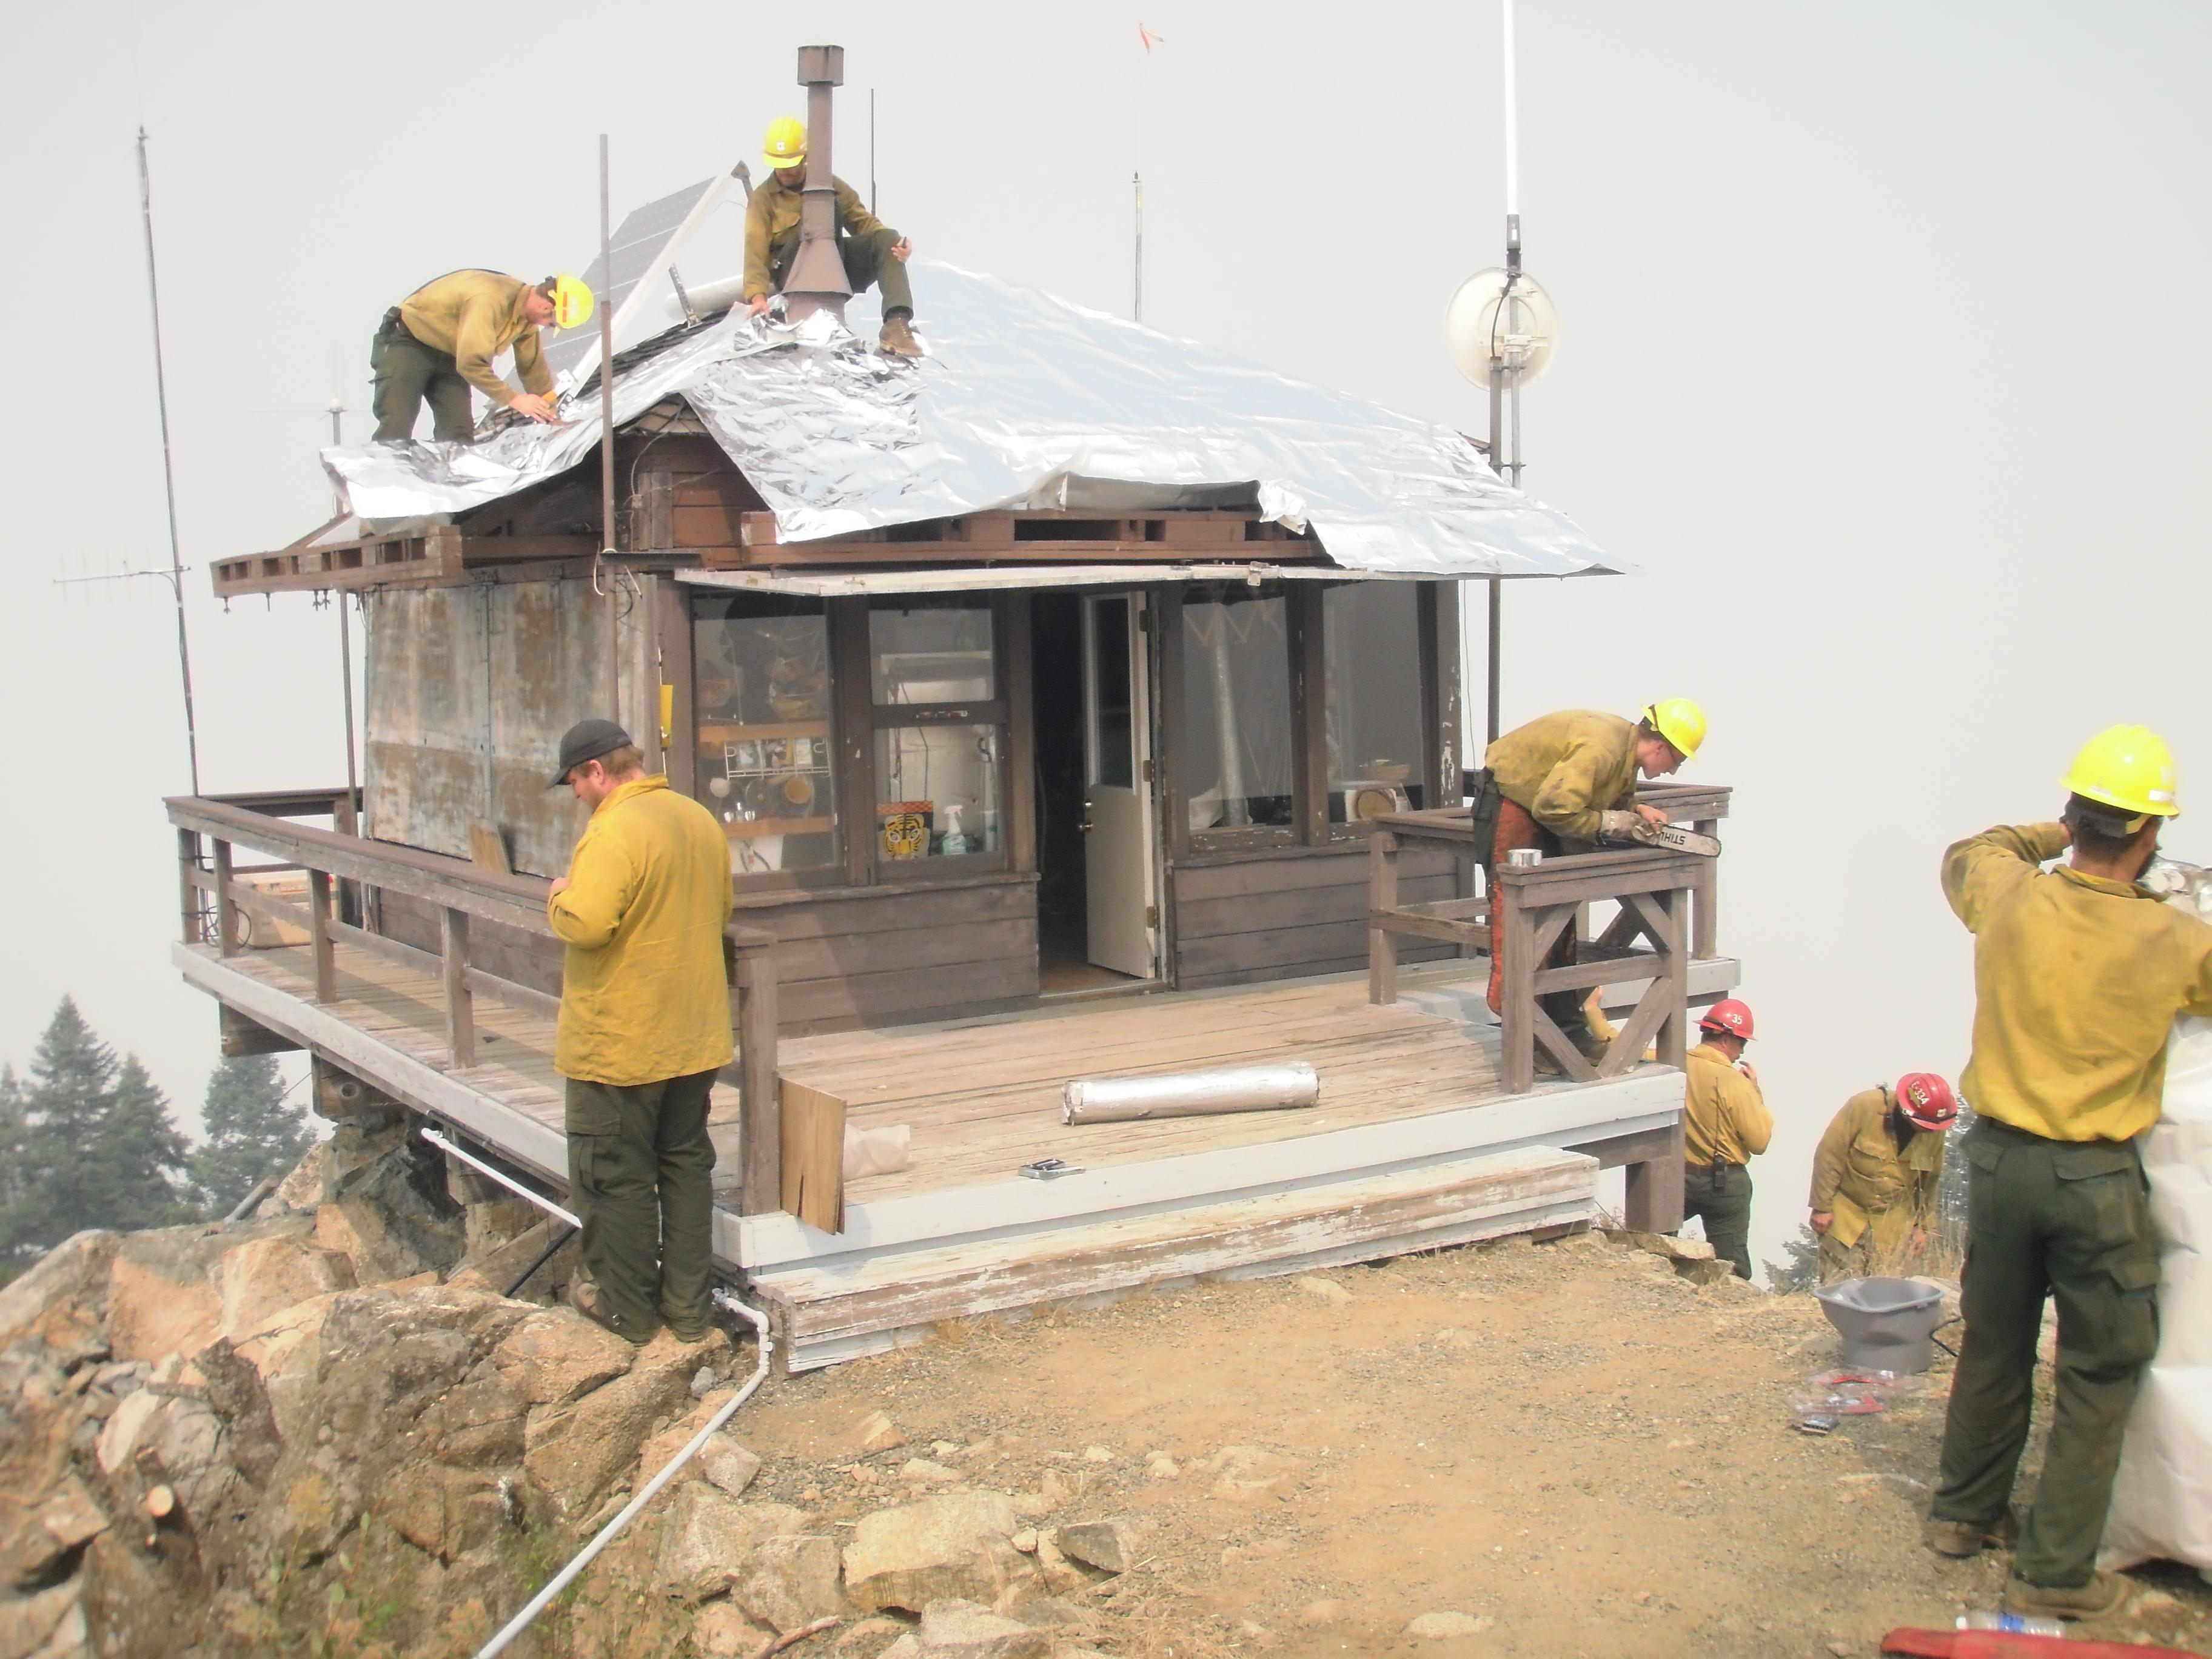
\includegraphics[scale=0.085]{images/ironside.jpg}
  \caption{The Ironside Mountain lookout and radio repeater station, destroyed in the 2021
    Monument fire, shown with protective foil on August
    $10^\textrm{th}$, 2015 during the 2015 River Complex fire. This
    particular fire burned 77,077 acres over 77 days. \textbf{CITATION NEEDED}}
  \label{fig:ironside}
\end{figure}

Use of centralized infrastructure comes with the potential for
widespread failure when the infrastructure breaks down. For example,
in California, the Ironside Mountain lookout/repeater station, seen in
Figure \ref{fig:ironside}, was destroyed during the 2021 Monument
Fire, which burned approximately 223,124 acres over 88 days
\cite{2021:monumentfire}. The Ironside Mountain station had strategic
importance, being located on a tall ridge. According to a video blog
from a volunteer firefighter involved in the incident\citationneeded,
its loss prevented communication between operators on different sides
of the ridge, in networking parlance creating a \emph{partition} that
lasted until crews could ascend the ridge to deploy a temporary
station:
\begin{quote}
  ``When {[}the Ironside Mountain lookout station{]} burned down the radio
  repeater went with it. And so communications were lost across the
  fire\ldots{} one side of the fire couldn't talk to the other side\ldots.
  So it was kind of a critical job to get that road cleared so that the
  radio crews could go back up there and set up a temporary radio tower.''
\end{quote}
A scenario where communication between two groups is completely
severed is exactly the sort of thing considered by the CAP theorem in
Section \ref{sec:background}.

\paragraph{Vehicles on the ground}
Large numbers of ground vehicles are involved in wildfire
suppression. A large wildfire response can involve up to 100
firetrucks distributed over a large geographical area. Bulldozers and
similar vehicles are also commonly used to control the landscape and
perimeter of the fire. An advantage of vehicles is that they can carry
heavier, which is to say better, communications equipment than a
human. For instance, a vehicle could be equipped with a satellite link
as well as a local wireless area network (WLAN) base station, serving
as a bridge between agents in the field and central coordinators
(e.g. incident commanders).

\paragraph{Communication in the air}

Wildland firefighting increasingly involves the use of helicopters and
fixed wing aircraft. Civil aviation has traditionally employed simpler
communication patterns than this use case demands. For instance,
aircraft equipped with Automatic Dependent Surveillance-Broadcast
(ADS-B) monitor their location using GPS and periodically broadcast
this information to air traffic controllers and nearby aircraft. This
sort of scheme has worked well in traditional applications, where
pilots typically only monitor the general locations of a few nearby
aircraft. The locality principle is exhibited here, too: aircraft have
the highest need to coordinate when they are physically close and
therefore in range of each other's ADS-B broadcasts.

In our setting, a large number or aircraft, easily a half dozen or
more, may need to operate in a small area, near complex terrain,
during adverse conditions, often at low altitude. In other words, the
demands are many and the margins for error are small. This sort of use
case calls for more sophisticated coordination schemes between
airborne and ground-based elements than solutions like ADS-B provide
by themselves.

As aircraft generally have better line-of-site to ground crews than
ground crews have to each other, firefighters sometimes relay messages
to air-based units over the radio, which in turn is relayed back down
to other ground units. The locality principle comes into play here
too, but this time in the reverse direction: this relay scheme allows
knowledge to travel farther but requires more effort, and the extended
reach comes at the cost of introducing delays and possible degradation
of message quality, as in the classic game of telephone. Hence, this
sort of message passing should be reserved for more critical
information.

In some cases, planes from the Civil Air
Patrol\citationneeded\footnote{A civil auxiliary of the U.S. Air
Force. https://www.gocivilairpatrol.com/} have been equipped with
radio repeaters and dispatched to wildfires to provide service to
ground-based units. In the future, this sort of service could be
provided autonomously by base stations mounted to unmanned aerial
vehicles (UAVs), which might perform additional functions such as
tracking the fire perimeter. More generally, future systems should
transparently facilitate exchanging information between agents in a
decentralized fashion that is robust to the failure of any one
component. In Section \ref{sec:networking} we imagine a resilient
ad-hoc digital network built from handheld and ground- and
air-vehicle-mounted devices, permanent base stations, portable
temporary infrastructure, and so on.
%---a high-tech modernization of the sort of informal relay schemes
%operating today over traditional radio channels.

\subsection{Towards the Future}\label{towards-the-future}

So far we have said a lot about the state of disaster response
today. A distributed system for this sort of challenge should be
designed for the kinds of environments and conditions expected in the
near- to medium-term future, so we briefly turn our attention to some
of our expectations for this topic.

Perhaps the most prominent expectation for future disaster response
events is a heavy reliance on \emph{data}. Besides improvements to
communications that facilitate information sharing, we expect advances
in machine intelligence to greatly influence how this data is
handled. Agents in disaster response environments will be both
producers and consumers of data, and this data will need to processed
by humans and machines in ways that agents can readily make sense of
to support their decision-making. Our background research indicated
many different kinds of data that could be valuable for
responders. Just some of the kinds of information and communication we
expect include the following:
\begin{itemize}
  \tightlist
\item
  Free-form communication, especially recorded voice messages
  broadcast to many agents at once, which may need to be processed by
  machines to extract the most pertinent information into a more
  actionable format
\item
  The exact or estimated location of victims, firefighters, vehicles,
  hazards, etc.
\item
  Medical information gathered from victims, perhaps stored in and
  collected from digital triage tags\citationneeded
\item
  Data about current and predicted fire or weather patterns
\item
  Topographic information about the terrain, highlighting for instance
  the location of rivers and roads that could form a fire control line
\item
  Planned escape routes, rendezvous points, safety zones, and landing
  zones
\item
  Availability and dispatching of assets, e.g.~ambulances, airtankers,
  or crews on standby\footnote{NOTE Need to mention Monares et al 2011}
\end{itemize}
In a perfect environment, such information would be shared with all
necessary agents in whole and instantly. In reality, agents will be
presented with information that is sometimes incomplete, out of date,
or contradictory---all problems that are further exacerbated by an
unreliable network. A superficially contradictory concern is that the
information presented will be \emph{overcomplete}, filled with petty
details that distract agents from their important tasks.

%Of course, there is no actual contradiction between incomplete
%information and information that is unneeded and useless at best.

In some ways, future systems for disaster response will bear
resemblence to future systems for warfighting, such as the conceptual
\emph{Internet of Battle Things} (IoBT) \citationneeded. Chiefly,
agents ``under extreme cognitive and physical stress'' will be subject
to a highly dynamic and dangerous environment. Various kinds of
technology will assist humans by providing data to support
sensemaking, but a contraindicating concern will be flooding agents with a
``massive, complex, confusing, and potentially
deceptive\footnote{While deliberately adversarial network behavior
seems like less of a concern for disaster response agents than
warfighters, we conjecture that a similar ``fog of war'' may
lead to confusing or contradictory reports that share similarities
with intentionally deceptive behavior.} ocean of information.'' To
avoid ``swimming in sensors and drowning in data''
\cite{2010:magnuson}:
\begin{quote}
``Humans seek well-formed, reasonably-sized, essential information
  that is highly relevant to their cognitive needs, such as effective
  indications and warnings that pertain to their current situation and
  mission.'' \citationneeded
\end{quote}
The most distinctive feature of the Internet of Battle Things, which
separates it from the everyday internet of things, is ``the
adversarial nature of the environment.'' To some extent this adversial
behavior is common also to disaster response. We previously cited a
real-world example of a critical communications station destroyed by
wildfire, perhaps not unlike an attack by enemy forces.

Lest we overstate the similarities between a battlefield environment
and civil disaster response, we expect that a distinctive feature of
the latter is a greater emphasis on the preservation of scarce network
resources. More so than a tactical military unit, a group of (say)
volunteer firefighters has to make do with off-the-shelf equipment
rather than purpose-built, best in class hardware like sophisticated
satellite links. Dedicated logistical support, and even things like
allocated radio frequencies, will likely be in shorter supply, while
adverse conditions like inclement weather will be almost
guaranteed. Therefore we expect a complex interaction between the
high-level needs of distributed applications and low-level concerns
about network resources. This is because only the applications have
enough information to determine which data is the most important and
must be shared with whom first, while only the network-level protocols
have enough information and control to make prudent use of scarce
network availability. In contravention to the common wisdom that
applications should be relatively blind to network considerations---or
conversely that network protocols ought to be transparent to
applications---our setting calls for mechanisms allowing the two
layers to have some influence over each other. This interaction
between the network and applications will be considered in more detail
in Sections \ref{sec:networking}, \ref{sec:continuous-consistency},
and \ref{sec:data-fusion}.

To give an example, a central data fusion center may be used to detect
and alert responders to a fire that has accidentally moved beyond a
control line (known as \emph{slopover}), or it may warn firefighters
when they have strayed too far from an escape route or safety
zone. Such information would be of high importance, and it would be
worthwhile to expend network resources conveying this information to
the relevant parties. It might also be nice for firefighters to have
access to real-time information about the GPS location of every other
firefighter. However, if this strains the network, then perhaps the
exact location of teammates, but only the general location of other
crews, is called for. If the network is extremely constrained, perhaps
only information immediately relevant to preserving life should be
sent in order to ensure the network is able to deliver this
information quickly. The key point is that from where we stand, we
cannot give a blanket rule determining which information is important,
as this is partly a dynamic calculation influenced both by the
criticality of the information to the task at hand and how much unused
network capacity is available at that moment at that location.

%For developers, it is clear that this requires some coordination
%between the application and the networking layers, as the latter must
%be given enough information to make the most prudent use of limited
%resources.

\section{Introduction to Distributed Systems}
\label{sec:background}
In this section we condense some of the main themes of distributed
systems theory and address how this fits into the picture painted in
Section \ref{sec:disaster-response}. The primary reference we are
following is the manuscript by Kshemkalyani and Singhal
\cite{kshemkalyani_singhal_2008}, particularly chapters 1, 3, 6, and
12.

A distributed system, in the most general sense, is a collection of
independent entities that cooperate to solve a problem that cannot be
individually solved \cite{kshemkalyani_singhal_2008}. This memo is
concerned with distributed systems used by firefighters and other
disaster response agents. The components of our system could be
computers, smartphones, sensors, or other kinds of communication
equipment, which may be carried by individuals, mounted to ground or
air-based vehicles, deployed as temporary or permanent infrastructure,
or attached to autonomous devices working alone or in tandem with
humans. The kinds of tasks our system might handle include navigating
safely in close proximity, delivering resources to remote locations,
suppressing fires, and collecting, processing, and disseminating data
about the environment.

Two major paradigms for thinking about distributed applications are
common: the message passing framework where the fundamental activity
is sending and receiving information over the network, or the more
abstract shared memory framework where the fundamental activity is
updating commonly held data items. In either case, a fundamental goal
for distributed computing systems is to ``{[}appear{]} to the users of
the system as a single coherent computer''
\cite{TanenbaumSteen07}. This means users of the system are presented
with the abstraction of a shared world, as if they are all connected
to a central omniscient computer rather than the complex system of
loosely coupled computers they are actually using.

\subsection{Message Passing}
\label{ssec:message-passing}

Singhal and Shivaratri \cite{10.5555/562065} offer the following
definition of a distributed computing system:

\begin{quote}
  ``A collection of computers that do not share common memory or a common
  physical clock, that communicate by message passing over a communication
  network, and where each computer has its own memory and runs its own
  operating system.''
\end{quote}
We shall consider a system consisting of a set \(\mathcal{P} =
\{P_i\}_{i\in I}\) of \emph{processes} executing on independent,
probably geographically dispersed computing devices, which we
consolidate under the generic term \emph{nodes}. It is important to
note that different kinds of nodes can have different characteristics,
such as capabilities and intended uses---in other words the system is
\emph{heterogeneous}---but for now we take a high-level view and treat
them simply as blackboxes that execute processes. A notable aspect of
what makes the system ``distributed'' is that the nodes must
communicate by passing messages, which must be facilitated by some
kind of network. This restriction is implied by absence of a common
memory (whereas processes running on the same machine can share
information by writing it to a common memory location).

A foundational assumption is that the network is never
perfect. Section \ref{sec:disaster-response} explained why this is
certainly expected in disaster scenarios. A primary challenge is that
delivering messages over the network is not instantaneous: message
packets must be sent over the air or through a cable and processed and
forwarded by any number of intermediate networking devices, and they
must be retransmitted in case of unrecoverable errors during transit,
all of which takes time. This means that messages are passed with some
unpredictable latency. In this section, our main challenge is to
provide ways for agents to coordinate their actions despite the
uncontrollable delays in communication caused by the network and
environment.

\paragraph{Network Reliability}
A priori, the network may not deliver a packet at all, i.e.~it may
silently discard messages without alerting the sender. The same
message may be also be delivered multiple times, and different
messages may arrive in any order. In the case of \emph{Byzantine
faults}\citationneeded, the network might even act like a malicious
adversary. In this section, being focused on higher-level
considerations, we shall assume that messages are delivered exactly
once, uncorrupted, but with an unpredictable delay. Some, but not all,
common so-called ``transport'' protocols like TCP\citationneeded and
LTP\citationneeded can provide this sort of semi-reliable message
delivery over a less reliable network. For example, these protocols
might tag outgoing messages with identifiers that allow the receiver
to detect duplicates and arrange messages in the order intended by the
sender, add checksums used to verify message integrity, and
transparently handle retranmission when messages become corrupted. We
shall take a closer look at these kinds of low-level details in
Section \ref{sec:networking}, where we relax our assumptions about
network reliability. For now, one could say we are working at a level
of abstraction above the network transport layer: the ``network'' is
just something that eventually delivers messages to the right people,
but not always at the right time, which is the problem. Note that
reliability mechanisms in transport-level protocols contribute to the
latency involved in communication, so they do not solve the problems
under consideration here, namely the difficulty of coordination when
messages are unpredictably delayed and nodes do not have access to
perfectly sychronized clocks.

\subsubsection{FIFO and causal ordering}

Figure \ref{fig:message-latencies} shows several time diagrams for
messages $\{m_i\}_{i=1}^N$ sent between three processes $P_1$, $P_2$,
and $P_3$. The $x$-axis of the diagram depicts the flow of physical
time from left to right. Each process consists of a worldline
depicting the \emph{events} occurring in that process. Each message
$m$ starts off as a message \emph{send} event $m^\textrm{send}$
indicating the moment the message is sent over the network by its
originating process; its delivery generates a message \emph{receive}
event $m^\textrm{recv}$. The send-receive event pairs are connected by
an arrow and said to be corresponding events. The subscripts on the
messages only serve to disambiguate them to the reader, but they are
not part of the message and have no semantic importance.

\begin{figure}[p]
  \setlength\belowcaptionskip{5ex}

  \begin{subfigure}{1\textwidth}
    \centering
    \begin{pgfpicture}
\pgfpathrectangle{\pgfpointorigin}{\pgfqpoint{390.0000bp}{154.0000bp}}
\pgfusepath{use as bounding box}
\begin{pgfscope}
\pgfsetlinewidth{1.0000bp}
\definecolor{sc}{rgb}{0.0000,0.0000,0.0000}
\pgfsetstrokecolor{sc}
\pgfsetmiterjoin
\pgfsetbuttcap
\pgfpathqmoveto{277.3427bp}{75.5915bp}
\pgfpathqlineto{339.0197bp}{26.2498bp}
\pgfusepathqstroke
\end{pgfscope}
\begin{pgfscope}
\definecolor{fc}{rgb}{0.0000,0.0000,0.0000}
\pgfsetfillcolor{fc}
\pgfusepathqfill
\end{pgfscope}
\begin{pgfscope}
\definecolor{fc}{rgb}{0.0000,0.0000,0.0000}
\pgfsetfillcolor{fc}
\pgfusepathqfill
\end{pgfscope}
\begin{pgfscope}
\definecolor{fc}{rgb}{0.0000,0.0000,0.0000}
\pgfsetfillcolor{fc}
\pgfpathqmoveto{345.7378bp}{20.8753bp}
\pgfpathqlineto{339.9249bp}{29.7111bp}
\pgfpathqlineto{339.2250bp}{26.0856bp}
\pgfpathqlineto{335.8416bp}{24.6069bp}
\pgfpathqlineto{345.7378bp}{20.8753bp}
\pgfpathclose
\pgfusepathqfill
\end{pgfscope}
\begin{pgfscope}
\definecolor{fc}{rgb}{0.0000,0.0000,0.0000}
\pgfsetfillcolor{fc}
\pgfpathqmoveto{339.2250bp}{26.0856bp}
\pgfpathqlineto{339.0197bp}{26.2498bp}
\pgfpathqlineto{339.3321bp}{26.6403bp}
\pgfpathqlineto{339.2250bp}{26.0856bp}
\pgfpathqlineto{339.0197bp}{26.2498bp}
\pgfpathqlineto{338.7074bp}{25.8594bp}
\pgfpathqlineto{339.2250bp}{26.0856bp}
\pgfpathclose
\pgfusepathqfill
\end{pgfscope}
\begin{pgfscope}
\pgfsetlinewidth{1.0000bp}
\definecolor{sc}{rgb}{0.0000,0.0000,0.0000}
\pgfsetstrokecolor{sc}
\pgfsetmiterjoin
\pgfsetbuttcap
\pgfpathqmoveto{172.0272bp}{135.2541bp}
\pgfpathqlineto{215.4983bp}{87.8311bp}
\pgfusepathqstroke
\end{pgfscope}
\begin{pgfscope}
\definecolor{fc}{rgb}{0.0000,0.0000,0.0000}
\pgfsetfillcolor{fc}
\pgfusepathqfill
\end{pgfscope}
\begin{pgfscope}
\definecolor{fc}{rgb}{0.0000,0.0000,0.0000}
\pgfsetfillcolor{fc}
\pgfusepathqfill
\end{pgfscope}
\begin{pgfscope}
\definecolor{fc}{rgb}{0.0000,0.0000,0.0000}
\pgfsetfillcolor{fc}
\pgfpathqmoveto{221.3118bp}{81.4891bp}
\pgfpathqlineto{216.9241bp}{91.1124bp}
\pgfpathqlineto{215.6759bp}{87.6374bp}
\pgfpathqlineto{212.1056bp}{86.6955bp}
\pgfpathqlineto{221.3118bp}{81.4891bp}
\pgfpathclose
\pgfusepathqfill
\end{pgfscope}
\begin{pgfscope}
\definecolor{fc}{rgb}{0.0000,0.0000,0.0000}
\pgfsetfillcolor{fc}
\pgfpathqmoveto{215.6759bp}{87.6374bp}
\pgfpathqlineto{215.4983bp}{87.8311bp}
\pgfpathqlineto{215.8669bp}{88.1690bp}
\pgfpathqlineto{215.6759bp}{87.6374bp}
\pgfpathqlineto{215.4983bp}{87.8311bp}
\pgfpathqlineto{215.1297bp}{87.4933bp}
\pgfpathqlineto{215.6759bp}{87.6374bp}
\pgfpathclose
\pgfusepathqfill
\end{pgfscope}
\begin{pgfscope}
\pgfsetlinewidth{1.0000bp}
\definecolor{sc}{rgb}{0.0000,0.0000,0.0000}
\pgfsetstrokecolor{sc}
\pgfsetmiterjoin
\pgfsetbuttcap
\pgfpathqmoveto{160.5252bp}{19.0860bp}
\pgfpathqlineto{333.1653bp}{129.8712bp}
\pgfusepathqstroke
\end{pgfscope}
\begin{pgfscope}
\definecolor{fc}{rgb}{0.0000,0.0000,0.0000}
\pgfsetfillcolor{fc}
\pgfusepathqfill
\end{pgfscope}
\begin{pgfscope}
\definecolor{fc}{rgb}{0.0000,0.0000,0.0000}
\pgfsetfillcolor{fc}
\pgfusepathqfill
\end{pgfscope}
\begin{pgfscope}
\definecolor{fc}{rgb}{0.0000,0.0000,0.0000}
\pgfsetfillcolor{fc}
\pgfpathqmoveto{340.4061bp}{134.5176bp}
\pgfpathqlineto{330.1753bp}{131.8358bp}
\pgfpathqlineto{333.3865bp}{130.0131bp}
\pgfpathqlineto{333.7055bp}{126.3345bp}
\pgfpathqlineto{340.4061bp}{134.5176bp}
\pgfpathclose
\pgfusepathqfill
\end{pgfscope}
\begin{pgfscope}
\definecolor{fc}{rgb}{0.0000,0.0000,0.0000}
\pgfsetfillcolor{fc}
\pgfpathqmoveto{333.3865bp}{130.0131bp}
\pgfpathqlineto{333.1653bp}{129.8712bp}
\pgfpathqlineto{332.8953bp}{130.2920bp}
\pgfpathqlineto{333.3865bp}{130.0131bp}
\pgfpathqlineto{333.1653bp}{129.8712bp}
\pgfpathqlineto{333.4353bp}{129.4503bp}
\pgfpathqlineto{333.3865bp}{130.0131bp}
\pgfpathclose
\pgfusepathqfill
\end{pgfscope}
\begin{pgfscope}
\pgfsetlinewidth{1.0000bp}
\definecolor{sc}{rgb}{0.0000,0.0000,0.0000}
\pgfsetstrokecolor{sc}
\pgfsetmiterjoin
\pgfsetbuttcap
\pgfpathqmoveto{82.6052bp}{135.9769bp}
\pgfpathqlineto{277.7907bp}{24.4423bp}
\pgfusepathqstroke
\end{pgfscope}
\begin{pgfscope}
\definecolor{fc}{rgb}{0.0000,0.0000,0.0000}
\pgfsetfillcolor{fc}
\pgfusepathqfill
\end{pgfscope}
\begin{pgfscope}
\definecolor{fc}{rgb}{0.0000,0.0000,0.0000}
\pgfsetfillcolor{fc}
\pgfusepathqfill
\end{pgfscope}
\begin{pgfscope}
\definecolor{fc}{rgb}{0.0000,0.0000,0.0000}
\pgfsetfillcolor{fc}
\pgfpathqmoveto{285.2606bp}{20.1739bp}
\pgfpathqlineto{278.1487bp}{28.0021bp}
\pgfpathqlineto{278.0190bp}{24.3119bp}
\pgfpathqlineto{274.9056bp}{22.3267bp}
\pgfpathqlineto{285.2606bp}{20.1739bp}
\pgfpathclose
\pgfusepathqfill
\end{pgfscope}
\begin{pgfscope}
\definecolor{fc}{rgb}{0.0000,0.0000,0.0000}
\pgfsetfillcolor{fc}
\pgfpathqmoveto{278.0190bp}{24.3119bp}
\pgfpathqlineto{277.7907bp}{24.4423bp}
\pgfpathqlineto{278.0388bp}{24.8765bp}
\pgfpathqlineto{278.0190bp}{24.3119bp}
\pgfpathqlineto{277.7907bp}{24.4423bp}
\pgfpathqlineto{277.5427bp}{24.0082bp}
\pgfpathqlineto{278.0190bp}{24.3119bp}
\pgfpathclose
\pgfusepathqfill
\end{pgfscope}
\begin{pgfscope}
\pgfsetlinewidth{1.0000bp}
\definecolor{sc}{rgb}{0.0000,0.0000,0.0000}
\pgfsetstrokecolor{sc}
\pgfsetmiterjoin
\pgfsetbuttcap
\pgfpathqmoveto{62.2044bp}{79.5005bp}
\pgfpathqlineto{114.6675bp}{127.9280bp}
\pgfusepathqstroke
\end{pgfscope}
\begin{pgfscope}
\definecolor{fc}{rgb}{0.0000,0.0000,0.0000}
\pgfsetfillcolor{fc}
\pgfusepathqfill
\end{pgfscope}
\begin{pgfscope}
\definecolor{fc}{rgb}{0.0000,0.0000,0.0000}
\pgfsetfillcolor{fc}
\pgfusepathqfill
\end{pgfscope}
\begin{pgfscope}
\definecolor{fc}{rgb}{0.0000,0.0000,0.0000}
\pgfsetfillcolor{fc}
\pgfpathqmoveto{120.9893bp}{133.7635bp}
\pgfpathqlineto{111.3813bp}{129.3424bp}
\pgfpathqlineto{114.8607bp}{128.1063bp}
\pgfpathqlineto{115.8149bp}{124.5393bp}
\pgfpathqlineto{120.9893bp}{133.7635bp}
\pgfpathclose
\pgfusepathqfill
\end{pgfscope}
\begin{pgfscope}
\definecolor{fc}{rgb}{0.0000,0.0000,0.0000}
\pgfsetfillcolor{fc}
\pgfpathqmoveto{114.8607bp}{128.1063bp}
\pgfpathqlineto{114.6675bp}{127.9280bp}
\pgfpathqlineto{114.3284bp}{128.2954bp}
\pgfpathqlineto{114.8607bp}{128.1063bp}
\pgfpathqlineto{114.6675bp}{127.9280bp}
\pgfpathqlineto{115.0067bp}{127.5606bp}
\pgfpathqlineto{114.8607bp}{128.1063bp}
\pgfpathclose
\pgfusepathqfill
\end{pgfscope}
\begin{pgfscope}
\pgfsetlinewidth{1.5000bp}
\definecolor{sc}{rgb}{0.0000,0.0000,0.0000}
\pgfsetstrokecolor{sc}
\pgfsetmiterjoin
\pgfsetbuttcap
\pgfpathqmoveto{30.0000bp}{17.4656bp}
\pgfpathqlineto{384.3463bp}{17.4656bp}
\pgfusepathqstroke
\end{pgfscope}
\begin{pgfscope}
\definecolor{fc}{rgb}{0.0000,0.0000,0.0000}
\pgfsetfillcolor{fc}
\pgfusepathqfill
\end{pgfscope}
\begin{pgfscope}
\definecolor{fc}{rgb}{0.0000,0.0000,0.0000}
\pgfsetfillcolor{fc}
\pgfusepathqfill
\end{pgfscope}
\begin{pgfscope}
\definecolor{fc}{rgb}{0.0000,0.0000,0.0000}
\pgfsetfillcolor{fc}
\pgfpathqmoveto{390.0000bp}{17.4656bp}
\pgfpathqlineto{384.3463bp}{20.7298bp}
\pgfpathqlineto{384.3463bp}{14.2015bp}
\pgfpathqlineto{390.0000bp}{17.4656bp}
\pgfpathclose
\pgfusepathqfill
\end{pgfscope}
\begin{pgfscope}
\definecolor{fc}{rgb}{0.0000,0.0000,0.0000}
\pgfsetfillcolor{fc}
\pgfusepathqfill
\end{pgfscope}
\begin{pgfscope}
\definecolor{fc}{rgb}{0.0000,0.0000,0.0000}
\pgfsetfillcolor{fc}
\pgfsetfillopacity{0.0000}
\pgfpathqmoveto{30.0000bp}{2.4656bp}
\pgfpathqlineto{30.0000bp}{32.4656bp}
\pgfpathqlineto{0.0000bp}{32.4656bp}
\pgfpathqlineto{-0.0000bp}{2.4656bp}
\pgfpathqlineto{30.0000bp}{2.4656bp}
\pgfpathclose
\pgfusepathqfill
\end{pgfscope}
\begin{pgfscope}
\pgftransformshift{\pgfqpoint{15.0000bp}{17.4656bp}}
\pgftext[base,left]{$P_3$}
\end{pgfscope}
\begin{pgfscope}
\pgftransformshift{\pgfqpoint{339.0601bp}{3.3446bp}}
\pgftext[base,left]{$\mrecv{5}$}
\end{pgfscope}
\begin{pgfscope}
\definecolor{fc}{rgb}{0.1216,0.4667,0.7059}
\pgfsetfillcolor{fc}
\pgfsetlinewidth{1.0000bp}
\definecolor{sc}{rgb}{0.0000,0.0000,0.0000}
\pgfsetstrokecolor{sc}
\pgfsetmiterjoin
\pgfsetbuttcap
\pgfpathqmoveto{353.0000bp}{17.4656bp}
\pgfpathqcurveto{353.0000bp}{19.1225bp}{351.6569bp}{20.4656bp}{350.0000bp}{20.4656bp}
\pgfpathqcurveto{348.3431bp}{20.4656bp}{347.0000bp}{19.1225bp}{347.0000bp}{17.4656bp}
\pgfpathqcurveto{347.0000bp}{15.8088bp}{348.3431bp}{14.4656bp}{350.0000bp}{14.4656bp}
\pgfpathqcurveto{351.6569bp}{14.4656bp}{353.0000bp}{15.8088bp}{353.0000bp}{17.4656bp}
\pgfpathclose
\pgfusepathqfillstroke
\end{pgfscope}
\begin{pgfscope}
\pgftransformshift{\pgfqpoint{279.0601bp}{3.3446bp}}
\pgftext[base,left]{$\mrecv{2}$}
\end{pgfscope}
\begin{pgfscope}
\definecolor{fc}{rgb}{0.1216,0.4667,0.7059}
\pgfsetfillcolor{fc}
\pgfsetlinewidth{1.0000bp}
\definecolor{sc}{rgb}{0.0000,0.0000,0.0000}
\pgfsetstrokecolor{sc}
\pgfsetmiterjoin
\pgfsetbuttcap
\pgfpathqmoveto{293.0000bp}{17.4656bp}
\pgfpathqcurveto{293.0000bp}{19.1225bp}{291.6569bp}{20.4656bp}{290.0000bp}{20.4656bp}
\pgfpathqcurveto{288.3431bp}{20.4656bp}{287.0000bp}{19.1225bp}{287.0000bp}{17.4656bp}
\pgfpathqcurveto{287.0000bp}{15.8088bp}{288.3431bp}{14.4656bp}{290.0000bp}{14.4656bp}
\pgfpathqcurveto{291.6569bp}{14.4656bp}{293.0000bp}{15.8088bp}{293.0000bp}{17.4656bp}
\pgfpathclose
\pgfusepathqfillstroke
\end{pgfscope}
\begin{pgfscope}
\pgftransformshift{\pgfqpoint{146.4843bp}{2.4729bp}}
\pgftext[base,left]{$\msend{3}$}
\end{pgfscope}
\begin{pgfscope}
\definecolor{fc}{rgb}{0.1216,0.4667,0.7059}
\pgfsetfillcolor{fc}
\pgfsetlinewidth{1.0000bp}
\definecolor{sc}{rgb}{0.0000,0.0000,0.0000}
\pgfsetstrokecolor{sc}
\pgfsetmiterjoin
\pgfsetbuttcap
\pgfpathqmoveto{161.0000bp}{17.4656bp}
\pgfpathqcurveto{161.0000bp}{19.1225bp}{159.6569bp}{20.4656bp}{158.0000bp}{20.4656bp}
\pgfpathqcurveto{156.3431bp}{20.4656bp}{155.0000bp}{19.1225bp}{155.0000bp}{17.4656bp}
\pgfpathqcurveto{155.0000bp}{15.8088bp}{156.3431bp}{14.4656bp}{158.0000bp}{14.4656bp}
\pgfpathqcurveto{159.6569bp}{14.4656bp}{161.0000bp}{15.8088bp}{161.0000bp}{17.4656bp}
\pgfpathclose
\pgfusepathqfillstroke
\end{pgfscope}
\begin{pgfscope}
\pgfsetlinewidth{1.5000bp}
\definecolor{sc}{rgb}{0.0000,0.0000,0.0000}
\pgfsetstrokecolor{sc}
\pgfsetmiterjoin
\pgfsetbuttcap
\pgfpathqmoveto{30.0000bp}{77.4656bp}
\pgfpathqlineto{384.3463bp}{77.4656bp}
\pgfusepathqstroke
\end{pgfscope}
\begin{pgfscope}
\definecolor{fc}{rgb}{0.0000,0.0000,0.0000}
\pgfsetfillcolor{fc}
\pgfusepathqfill
\end{pgfscope}
\begin{pgfscope}
\definecolor{fc}{rgb}{0.0000,0.0000,0.0000}
\pgfsetfillcolor{fc}
\pgfusepathqfill
\end{pgfscope}
\begin{pgfscope}
\definecolor{fc}{rgb}{0.0000,0.0000,0.0000}
\pgfsetfillcolor{fc}
\pgfpathqmoveto{390.0000bp}{77.4656bp}
\pgfpathqlineto{384.3463bp}{80.7298bp}
\pgfpathqlineto{384.3463bp}{74.2015bp}
\pgfpathqlineto{390.0000bp}{77.4656bp}
\pgfpathclose
\pgfusepathqfill
\end{pgfscope}
\begin{pgfscope}
\definecolor{fc}{rgb}{0.0000,0.0000,0.0000}
\pgfsetfillcolor{fc}
\pgfusepathqfill
\end{pgfscope}
\begin{pgfscope}
\definecolor{fc}{rgb}{0.0000,0.0000,0.0000}
\pgfsetfillcolor{fc}
\pgfsetfillopacity{0.0000}
\pgfpathqmoveto{30.0000bp}{62.4656bp}
\pgfpathqlineto{30.0000bp}{92.4656bp}
\pgfpathqlineto{0.0000bp}{92.4656bp}
\pgfpathqlineto{-0.0000bp}{62.4656bp}
\pgfpathqlineto{30.0000bp}{62.4656bp}
\pgfpathclose
\pgfusepathqfill
\end{pgfscope}
\begin{pgfscope}
\pgftransformshift{\pgfqpoint{15.0000bp}{77.4656bp}}
\pgftext[base,left]{$P_2$}
\end{pgfscope}
\begin{pgfscope}
\pgftransformshift{\pgfqpoint{276.2123bp}{87.2008bp}}
\pgftext[base,left]{$\msend{5}$}
\end{pgfscope}
\begin{pgfscope}
\definecolor{fc}{rgb}{0.1216,0.4667,0.7059}
\pgfsetfillcolor{fc}
\pgfsetlinewidth{1.0000bp}
\definecolor{sc}{rgb}{0.0000,0.0000,0.0000}
\pgfsetstrokecolor{sc}
\pgfsetmiterjoin
\pgfsetbuttcap
\pgfpathqmoveto{278.0000bp}{77.4656bp}
\pgfpathqcurveto{278.0000bp}{79.1225bp}{276.6569bp}{80.4656bp}{275.0000bp}{80.4656bp}
\pgfpathqcurveto{273.3431bp}{80.4656bp}{272.0000bp}{79.1225bp}{272.0000bp}{77.4656bp}
\pgfpathqcurveto{272.0000bp}{75.8088bp}{273.3431bp}{74.4656bp}{275.0000bp}{74.4656bp}
\pgfpathqcurveto{276.6569bp}{74.4656bp}{278.0000bp}{75.8088bp}{278.0000bp}{77.4656bp}
\pgfpathclose
\pgfusepathqfillstroke
\end{pgfscope}
\begin{pgfscope}
\pgftransformshift{\pgfqpoint{226.7880bp}{88.0725bp}}
\pgftext[base,left]{$\mrecv{4}$}
\end{pgfscope}
\begin{pgfscope}
\definecolor{fc}{rgb}{0.1216,0.4667,0.7059}
\pgfsetfillcolor{fc}
\pgfsetlinewidth{1.0000bp}
\definecolor{sc}{rgb}{0.0000,0.0000,0.0000}
\pgfsetstrokecolor{sc}
\pgfsetmiterjoin
\pgfsetbuttcap
\pgfpathqmoveto{228.0000bp}{77.4656bp}
\pgfpathqcurveto{228.0000bp}{79.1225bp}{226.6569bp}{80.4656bp}{225.0000bp}{80.4656bp}
\pgfpathqcurveto{223.3431bp}{80.4656bp}{222.0000bp}{79.1225bp}{222.0000bp}{77.4656bp}
\pgfpathqcurveto{222.0000bp}{75.8088bp}{223.3431bp}{74.4656bp}{225.0000bp}{74.4656bp}
\pgfpathqcurveto{226.6569bp}{74.4656bp}{228.0000bp}{75.8088bp}{228.0000bp}{77.4656bp}
\pgfpathclose
\pgfusepathqfillstroke
\end{pgfscope}
\begin{pgfscope}
\pgftransformshift{\pgfqpoint{48.4843bp}{62.4729bp}}
\pgftext[base,left]{$\msend{1}$}
\end{pgfscope}
\begin{pgfscope}
\definecolor{fc}{rgb}{0.1216,0.4667,0.7059}
\pgfsetfillcolor{fc}
\pgfsetlinewidth{1.0000bp}
\definecolor{sc}{rgb}{0.0000,0.0000,0.0000}
\pgfsetstrokecolor{sc}
\pgfsetmiterjoin
\pgfsetbuttcap
\pgfpathqmoveto{63.0000bp}{77.4656bp}
\pgfpathqcurveto{63.0000bp}{79.1225bp}{61.6569bp}{80.4656bp}{60.0000bp}{80.4656bp}
\pgfpathqcurveto{58.3431bp}{80.4656bp}{57.0000bp}{79.1225bp}{57.0000bp}{77.4656bp}
\pgfpathqcurveto{57.0000bp}{75.8088bp}{58.3431bp}{74.4656bp}{60.0000bp}{74.4656bp}
\pgfpathqcurveto{61.6569bp}{74.4656bp}{63.0000bp}{75.8088bp}{63.0000bp}{77.4656bp}
\pgfpathclose
\pgfusepathqfillstroke
\end{pgfscope}
\begin{pgfscope}
\pgfsetlinewidth{1.5000bp}
\definecolor{sc}{rgb}{0.0000,0.0000,0.0000}
\pgfsetstrokecolor{sc}
\pgfsetmiterjoin
\pgfsetbuttcap
\pgfpathqmoveto{30.0000bp}{137.4656bp}
\pgfpathqlineto{384.3463bp}{137.4656bp}
\pgfusepathqstroke
\end{pgfscope}
\begin{pgfscope}
\definecolor{fc}{rgb}{0.0000,0.0000,0.0000}
\pgfsetfillcolor{fc}
\pgfusepathqfill
\end{pgfscope}
\begin{pgfscope}
\definecolor{fc}{rgb}{0.0000,0.0000,0.0000}
\pgfsetfillcolor{fc}
\pgfusepathqfill
\end{pgfscope}
\begin{pgfscope}
\definecolor{fc}{rgb}{0.0000,0.0000,0.0000}
\pgfsetfillcolor{fc}
\pgfpathqmoveto{390.0000bp}{137.4656bp}
\pgfpathqlineto{384.3463bp}{140.7298bp}
\pgfpathqlineto{384.3463bp}{134.2015bp}
\pgfpathqlineto{390.0000bp}{137.4656bp}
\pgfpathclose
\pgfusepathqfill
\end{pgfscope}
\begin{pgfscope}
\definecolor{fc}{rgb}{0.0000,0.0000,0.0000}
\pgfsetfillcolor{fc}
\pgfusepathqfill
\end{pgfscope}
\begin{pgfscope}
\definecolor{fc}{rgb}{0.0000,0.0000,0.0000}
\pgfsetfillcolor{fc}
\pgfsetfillopacity{0.0000}
\pgfpathqmoveto{30.0000bp}{122.4656bp}
\pgfpathqlineto{30.0000bp}{152.4656bp}
\pgfpathqlineto{0.0000bp}{152.4656bp}
\pgfpathqlineto{-0.0000bp}{122.4656bp}
\pgfpathqlineto{30.0000bp}{122.4656bp}
\pgfpathclose
\pgfusepathqfill
\end{pgfscope}
\begin{pgfscope}
\pgftransformshift{\pgfqpoint{15.0000bp}{137.4656bp}}
\pgftext[base,left]{$P_1$}
\end{pgfscope}
\begin{pgfscope}
\pgftransformshift{\pgfqpoint{334.0601bp}{147.3446bp}}
\pgftext[base,left]{$\mrecv{3}$}
\end{pgfscope}
\begin{pgfscope}
\definecolor{fc}{rgb}{0.1216,0.4667,0.7059}
\pgfsetfillcolor{fc}
\pgfsetlinewidth{1.0000bp}
\definecolor{sc}{rgb}{0.0000,0.0000,0.0000}
\pgfsetstrokecolor{sc}
\pgfsetmiterjoin
\pgfsetbuttcap
\pgfpathqmoveto{348.0000bp}{137.4656bp}
\pgfpathqcurveto{348.0000bp}{139.1225bp}{346.6569bp}{140.4656bp}{345.0000bp}{140.4656bp}
\pgfpathqcurveto{343.3431bp}{140.4656bp}{342.0000bp}{139.1225bp}{342.0000bp}{137.4656bp}
\pgfpathqcurveto{342.0000bp}{135.8088bp}{343.3431bp}{134.4656bp}{345.0000bp}{134.4656bp}
\pgfpathqcurveto{346.6569bp}{134.4656bp}{348.0000bp}{135.8088bp}{348.0000bp}{137.4656bp}
\pgfpathclose
\pgfusepathqfillstroke
\end{pgfscope}
\begin{pgfscope}
\pgftransformshift{\pgfqpoint{158.4843bp}{146.4729bp}}
\pgftext[base,left]{$\msend{4}$}
\end{pgfscope}
\begin{pgfscope}
\definecolor{fc}{rgb}{0.1216,0.4667,0.7059}
\pgfsetfillcolor{fc}
\pgfsetlinewidth{1.0000bp}
\definecolor{sc}{rgb}{0.0000,0.0000,0.0000}
\pgfsetstrokecolor{sc}
\pgfsetmiterjoin
\pgfsetbuttcap
\pgfpathqmoveto{173.0000bp}{137.4656bp}
\pgfpathqcurveto{173.0000bp}{139.1225bp}{171.6569bp}{140.4656bp}{170.0000bp}{140.4656bp}
\pgfpathqcurveto{168.3431bp}{140.4656bp}{167.0000bp}{139.1225bp}{167.0000bp}{137.4656bp}
\pgfpathqcurveto{167.0000bp}{135.8088bp}{168.3431bp}{134.4656bp}{170.0000bp}{134.4656bp}
\pgfpathqcurveto{171.6569bp}{134.4656bp}{173.0000bp}{135.8088bp}{173.0000bp}{137.4656bp}
\pgfpathclose
\pgfusepathqfillstroke
\end{pgfscope}
\begin{pgfscope}
\pgftransformshift{\pgfqpoint{114.0601bp}{147.3446bp}}
\pgftext[base,left]{$\mrecv{1}$}
\end{pgfscope}
\begin{pgfscope}
\definecolor{fc}{rgb}{0.1216,0.4667,0.7059}
\pgfsetfillcolor{fc}
\pgfsetlinewidth{1.0000bp}
\definecolor{sc}{rgb}{0.0000,0.0000,0.0000}
\pgfsetstrokecolor{sc}
\pgfsetmiterjoin
\pgfsetbuttcap
\pgfpathqmoveto{128.0000bp}{137.4656bp}
\pgfpathqcurveto{128.0000bp}{139.1225bp}{126.6569bp}{140.4656bp}{125.0000bp}{140.4656bp}
\pgfpathqcurveto{123.3431bp}{140.4656bp}{122.0000bp}{139.1225bp}{122.0000bp}{137.4656bp}
\pgfpathqcurveto{122.0000bp}{135.8088bp}{123.3431bp}{134.4656bp}{125.0000bp}{134.4656bp}
\pgfpathqcurveto{126.6569bp}{134.4656bp}{128.0000bp}{135.8088bp}{128.0000bp}{137.4656bp}
\pgfpathclose
\pgfusepathqfillstroke
\end{pgfscope}
\begin{pgfscope}
\pgftransformshift{\pgfqpoint{68.4843bp}{146.4729bp}}
\pgftext[base,left]{$\msend{2}$}
\end{pgfscope}
\begin{pgfscope}
\definecolor{fc}{rgb}{0.1216,0.4667,0.7059}
\pgfsetfillcolor{fc}
\pgfsetlinewidth{1.0000bp}
\definecolor{sc}{rgb}{0.0000,0.0000,0.0000}
\pgfsetstrokecolor{sc}
\pgfsetmiterjoin
\pgfsetbuttcap
\pgfpathqmoveto{83.0000bp}{137.4656bp}
\pgfpathqcurveto{83.0000bp}{139.1225bp}{81.6569bp}{140.4656bp}{80.0000bp}{140.4656bp}
\pgfpathqcurveto{78.3431bp}{140.4656bp}{77.0000bp}{139.1225bp}{77.0000bp}{137.4656bp}
\pgfpathqcurveto{77.0000bp}{135.8088bp}{78.3431bp}{134.4656bp}{80.0000bp}{134.4656bp}
\pgfpathqcurveto{81.6569bp}{134.4656bp}{83.0000bp}{135.8088bp}{83.0000bp}{137.4656bp}
\pgfpathclose
\pgfusepathqfillstroke
\end{pgfscope}
\end{pgfpicture}

    \caption{Depiction of latencies in message passing}
    \label{fig:message-latencies-a}
  \end{subfigure}

  \begin{subfigure}{1\textwidth}
    \centering \begin{pgfpicture}
\pgfpathrectangle{\pgfpointorigin}{\pgfqpoint{390.0000bp}{154.0000bp}}
\pgfusepath{use as bounding box}
\begin{pgfscope}
\pgfsetlinewidth{1.0000bp}
\definecolor{sc}{rgb}{0.0000,0.0000,0.0000}
\pgfsetstrokecolor{sc}
\pgfsetmiterjoin
\pgfsetbuttcap
\pgfpathqmoveto{321.3419bp}{134.7818bp}
\pgfpathqlineto{343.7112bp}{90.0432bp}
\pgfusepathqstroke
\end{pgfscope}
\begin{pgfscope}
\definecolor{fc}{rgb}{0.0000,0.0000,0.0000}
\pgfsetfillcolor{fc}
\pgfusepathqfill
\end{pgfscope}
\begin{pgfscope}
\definecolor{fc}{rgb}{0.0000,0.0000,0.0000}
\pgfsetfillcolor{fc}
\pgfusepathqfill
\end{pgfscope}
\begin{pgfscope}
\definecolor{fc}{rgb}{0.0000,0.0000,0.0000}
\pgfsetfillcolor{fc}
\pgfpathqmoveto{347.5588bp}{82.3481bp}
\pgfpathqlineto{345.9836bp}{92.8066bp}
\pgfpathqlineto{343.8288bp}{89.8081bp}
\pgfpathqlineto{340.1371bp}{89.8833bp}
\pgfpathqlineto{347.5588bp}{82.3481bp}
\pgfpathclose
\pgfusepathqfill
\end{pgfscope}
\begin{pgfscope}
\definecolor{fc}{rgb}{0.0000,0.0000,0.0000}
\pgfsetfillcolor{fc}
\pgfpathqmoveto{343.8288bp}{89.8081bp}
\pgfpathqlineto{343.7112bp}{90.0432bp}
\pgfpathqlineto{344.1584bp}{90.2668bp}
\pgfpathqlineto{343.8288bp}{89.8081bp}
\pgfpathqlineto{343.7112bp}{90.0432bp}
\pgfpathqlineto{343.2640bp}{89.8196bp}
\pgfpathqlineto{343.8288bp}{89.8081bp}
\pgfpathclose
\pgfusepathqfill
\end{pgfscope}
\begin{pgfscope}
\pgfsetlinewidth{1.0000bp}
\definecolor{sc}{rgb}{0.0000,0.0000,0.0000}
\pgfsetstrokecolor{sc}
\pgfsetmiterjoin
\pgfsetbuttcap
\pgfpathqmoveto{261.3419bp}{80.1495bp}
\pgfpathqlineto{283.7112bp}{124.8880bp}
\pgfusepathqstroke
\end{pgfscope}
\begin{pgfscope}
\definecolor{fc}{rgb}{0.0000,0.0000,0.0000}
\pgfsetfillcolor{fc}
\pgfusepathqfill
\end{pgfscope}
\begin{pgfscope}
\definecolor{fc}{rgb}{0.0000,0.0000,0.0000}
\pgfsetfillcolor{fc}
\pgfusepathqfill
\end{pgfscope}
\begin{pgfscope}
\definecolor{fc}{rgb}{0.0000,0.0000,0.0000}
\pgfsetfillcolor{fc}
\pgfpathqmoveto{287.5588bp}{132.5831bp}
\pgfpathqlineto{280.1371bp}{125.0479bp}
\pgfpathqlineto{283.8288bp}{125.1232bp}
\pgfpathqlineto{285.9836bp}{122.1247bp}
\pgfpathqlineto{287.5588bp}{132.5831bp}
\pgfpathclose
\pgfusepathqfill
\end{pgfscope}
\begin{pgfscope}
\definecolor{fc}{rgb}{0.0000,0.0000,0.0000}
\pgfsetfillcolor{fc}
\pgfpathqmoveto{283.8288bp}{125.1232bp}
\pgfpathqlineto{283.7112bp}{124.8880bp}
\pgfpathqlineto{283.2640bp}{125.1116bp}
\pgfpathqlineto{283.8288bp}{125.1232bp}
\pgfpathqlineto{283.7112bp}{124.8880bp}
\pgfpathqlineto{284.1584bp}{124.6644bp}
\pgfpathqlineto{283.8288bp}{125.1232bp}
\pgfpathclose
\pgfusepathqfill
\end{pgfscope}
\begin{pgfscope}
\pgfsetlinewidth{1.0000bp}
\definecolor{sc}{rgb}{0.0000,0.0000,0.0000}
\pgfsetstrokecolor{sc}
\pgfsetmiterjoin
\pgfsetbuttcap
\pgfpathqmoveto{171.3419bp}{134.7818bp}
\pgfpathqlineto{193.7112bp}{90.0432bp}
\pgfusepathqstroke
\end{pgfscope}
\begin{pgfscope}
\definecolor{fc}{rgb}{0.0000,0.0000,0.0000}
\pgfsetfillcolor{fc}
\pgfusepathqfill
\end{pgfscope}
\begin{pgfscope}
\definecolor{fc}{rgb}{0.0000,0.0000,0.0000}
\pgfsetfillcolor{fc}
\pgfusepathqfill
\end{pgfscope}
\begin{pgfscope}
\definecolor{fc}{rgb}{0.0000,0.0000,0.0000}
\pgfsetfillcolor{fc}
\pgfpathqmoveto{197.5588bp}{82.3481bp}
\pgfpathqlineto{195.9836bp}{92.8066bp}
\pgfpathqlineto{193.8288bp}{89.8081bp}
\pgfpathqlineto{190.1371bp}{89.8833bp}
\pgfpathqlineto{197.5588bp}{82.3481bp}
\pgfpathclose
\pgfusepathqfill
\end{pgfscope}
\begin{pgfscope}
\definecolor{fc}{rgb}{0.0000,0.0000,0.0000}
\pgfsetfillcolor{fc}
\pgfpathqmoveto{193.8288bp}{89.8081bp}
\pgfpathqlineto{193.7112bp}{90.0432bp}
\pgfpathqlineto{194.1584bp}{90.2668bp}
\pgfpathqlineto{193.8288bp}{89.8081bp}
\pgfpathqlineto{193.7112bp}{90.0432bp}
\pgfpathqlineto{193.2640bp}{89.8196bp}
\pgfpathqlineto{193.8288bp}{89.8081bp}
\pgfpathclose
\pgfusepathqfill
\end{pgfscope}
\begin{pgfscope}
\pgfsetlinewidth{1.0000bp}
\definecolor{sc}{rgb}{0.0000,0.0000,0.0000}
\pgfsetstrokecolor{sc}
\pgfsetmiterjoin
\pgfsetbuttcap
\pgfpathqmoveto{111.3419bp}{80.1495bp}
\pgfpathqlineto{133.7112bp}{124.8880bp}
\pgfusepathqstroke
\end{pgfscope}
\begin{pgfscope}
\definecolor{fc}{rgb}{0.0000,0.0000,0.0000}
\pgfsetfillcolor{fc}
\pgfusepathqfill
\end{pgfscope}
\begin{pgfscope}
\definecolor{fc}{rgb}{0.0000,0.0000,0.0000}
\pgfsetfillcolor{fc}
\pgfusepathqfill
\end{pgfscope}
\begin{pgfscope}
\definecolor{fc}{rgb}{0.0000,0.0000,0.0000}
\pgfsetfillcolor{fc}
\pgfpathqmoveto{137.5588bp}{132.5831bp}
\pgfpathqlineto{130.1371bp}{125.0479bp}
\pgfpathqlineto{133.8288bp}{125.1232bp}
\pgfpathqlineto{135.9836bp}{122.1247bp}
\pgfpathqlineto{137.5588bp}{132.5831bp}
\pgfpathclose
\pgfusepathqfill
\end{pgfscope}
\begin{pgfscope}
\definecolor{fc}{rgb}{0.0000,0.0000,0.0000}
\pgfsetfillcolor{fc}
\pgfpathqmoveto{133.8288bp}{125.1232bp}
\pgfpathqlineto{133.7112bp}{124.8880bp}
\pgfpathqlineto{133.2640bp}{125.1116bp}
\pgfpathqlineto{133.8288bp}{125.1232bp}
\pgfpathqlineto{133.7112bp}{124.8880bp}
\pgfpathqlineto{134.1584bp}{124.6644bp}
\pgfpathqlineto{133.8288bp}{125.1232bp}
\pgfpathclose
\pgfusepathqfill
\end{pgfscope}
\begin{pgfscope}
\pgfsetlinewidth{1.0000bp}
\definecolor{sc}{rgb}{0.0000,0.0000,0.0000}
\pgfsetstrokecolor{sc}
\pgfsetmiterjoin
\pgfsetbuttcap
\pgfpathqmoveto{51.3419bp}{134.7818bp}
\pgfpathqlineto{73.7112bp}{90.0432bp}
\pgfusepathqstroke
\end{pgfscope}
\begin{pgfscope}
\definecolor{fc}{rgb}{0.0000,0.0000,0.0000}
\pgfsetfillcolor{fc}
\pgfusepathqfill
\end{pgfscope}
\begin{pgfscope}
\definecolor{fc}{rgb}{0.0000,0.0000,0.0000}
\pgfsetfillcolor{fc}
\pgfusepathqfill
\end{pgfscope}
\begin{pgfscope}
\definecolor{fc}{rgb}{0.0000,0.0000,0.0000}
\pgfsetfillcolor{fc}
\pgfpathqmoveto{77.5588bp}{82.3481bp}
\pgfpathqlineto{75.9836bp}{92.8066bp}
\pgfpathqlineto{73.8288bp}{89.8081bp}
\pgfpathqlineto{70.1371bp}{89.8833bp}
\pgfpathqlineto{77.5588bp}{82.3481bp}
\pgfpathclose
\pgfusepathqfill
\end{pgfscope}
\begin{pgfscope}
\definecolor{fc}{rgb}{0.0000,0.0000,0.0000}
\pgfsetfillcolor{fc}
\pgfpathqmoveto{73.8288bp}{89.8081bp}
\pgfpathqlineto{73.7112bp}{90.0432bp}
\pgfpathqlineto{74.1584bp}{90.2668bp}
\pgfpathqlineto{73.8288bp}{89.8081bp}
\pgfpathqlineto{73.7112bp}{90.0432bp}
\pgfpathqlineto{73.2640bp}{89.8196bp}
\pgfpathqlineto{73.8288bp}{89.8081bp}
\pgfpathclose
\pgfusepathqfill
\end{pgfscope}
\begin{pgfscope}
\pgfsetlinewidth{1.0000bp}
\definecolor{sc}{rgb}{0.0000,0.0000,0.0000}
\pgfsetstrokecolor{sc}
\pgfsetmiterjoin
\pgfsetbuttcap
\pgfpathqmoveto{42.8201bp}{18.4911bp}
\pgfpathqlineto{356.7843bp}{132.6599bp}
\pgfusepathqstroke
\end{pgfscope}
\begin{pgfscope}
\definecolor{fc}{rgb}{0.0000,0.0000,0.0000}
\pgfsetfillcolor{fc}
\pgfusepathqfill
\end{pgfscope}
\begin{pgfscope}
\definecolor{fc}{rgb}{0.0000,0.0000,0.0000}
\pgfsetfillcolor{fc}
\pgfusepathqfill
\end{pgfscope}
\begin{pgfscope}
\definecolor{fc}{rgb}{0.0000,0.0000,0.0000}
\pgfsetfillcolor{fc}
\pgfpathqmoveto{364.8697bp}{135.6001bp}
\pgfpathqlineto{354.2996bp}{135.2341bp}
\pgfpathqlineto{357.0314bp}{132.7497bp}
\pgfpathqlineto{356.5335bp}{129.0910bp}
\pgfpathqlineto{364.8697bp}{135.6001bp}
\pgfpathclose
\pgfusepathqfill
\end{pgfscope}
\begin{pgfscope}
\definecolor{fc}{rgb}{0.0000,0.0000,0.0000}
\pgfsetfillcolor{fc}
\pgfpathqmoveto{357.0314bp}{132.7497bp}
\pgfpathqlineto{356.7843bp}{132.6599bp}
\pgfpathqlineto{356.6134bp}{133.1298bp}
\pgfpathqlineto{357.0314bp}{132.7497bp}
\pgfpathqlineto{356.7843bp}{132.6599bp}
\pgfpathqlineto{356.9552bp}{132.1900bp}
\pgfpathqlineto{357.0314bp}{132.7497bp}
\pgfpathclose
\pgfusepathqfill
\end{pgfscope}
\begin{pgfscope}
\pgfsetlinewidth{1.5000bp}
\definecolor{sc}{rgb}{0.0000,0.0000,0.0000}
\pgfsetstrokecolor{sc}
\pgfsetmiterjoin
\pgfsetbuttcap
\pgfpathqmoveto{30.0000bp}{17.4656bp}
\pgfpathqlineto{384.3463bp}{17.4656bp}
\pgfusepathqstroke
\end{pgfscope}
\begin{pgfscope}
\definecolor{fc}{rgb}{0.0000,0.0000,0.0000}
\pgfsetfillcolor{fc}
\pgfusepathqfill
\end{pgfscope}
\begin{pgfscope}
\definecolor{fc}{rgb}{0.0000,0.0000,0.0000}
\pgfsetfillcolor{fc}
\pgfusepathqfill
\end{pgfscope}
\begin{pgfscope}
\definecolor{fc}{rgb}{0.0000,0.0000,0.0000}
\pgfsetfillcolor{fc}
\pgfpathqmoveto{390.0000bp}{17.4656bp}
\pgfpathqlineto{384.3463bp}{20.7298bp}
\pgfpathqlineto{384.3463bp}{14.2015bp}
\pgfpathqlineto{390.0000bp}{17.4656bp}
\pgfpathclose
\pgfusepathqfill
\end{pgfscope}
\begin{pgfscope}
\definecolor{fc}{rgb}{0.0000,0.0000,0.0000}
\pgfsetfillcolor{fc}
\pgfusepathqfill
\end{pgfscope}
\begin{pgfscope}
\definecolor{fc}{rgb}{0.0000,0.0000,0.0000}
\pgfsetfillcolor{fc}
\pgfsetfillopacity{0.0000}
\pgfpathqmoveto{30.0000bp}{2.4656bp}
\pgfpathqlineto{30.0000bp}{32.4656bp}
\pgfpathqlineto{0.0000bp}{32.4656bp}
\pgfpathqlineto{-0.0000bp}{2.4656bp}
\pgfpathqlineto{30.0000bp}{2.4656bp}
\pgfpathclose
\pgfusepathqfill
\end{pgfscope}
\begin{pgfscope}
\pgftransformshift{\pgfqpoint{15.0000bp}{17.4656bp}}
\pgftext[base,left]{$P_3$}
\end{pgfscope}
\begin{pgfscope}
\pgftransformshift{\pgfqpoint{27.6277bp}{2.4729bp}}
\pgftext[base,left]{$m_1^\textrm{send}$}
\end{pgfscope}
\begin{pgfscope}
\definecolor{fc}{rgb}{0.1216,0.4667,0.7059}
\pgfsetfillcolor{fc}
\pgfsetlinewidth{1.0000bp}
\definecolor{sc}{rgb}{0.0000,0.0000,0.0000}
\pgfsetstrokecolor{sc}
\pgfsetmiterjoin
\pgfsetbuttcap
\pgfpathqmoveto{43.0000bp}{17.4656bp}
\pgfpathqcurveto{43.0000bp}{19.1225bp}{41.6569bp}{20.4656bp}{40.0000bp}{20.4656bp}
\pgfpathqcurveto{38.3431bp}{20.4656bp}{37.0000bp}{19.1225bp}{37.0000bp}{17.4656bp}
\pgfpathqcurveto{37.0000bp}{15.8088bp}{38.3431bp}{14.4656bp}{40.0000bp}{14.4656bp}
\pgfpathqcurveto{41.6569bp}{14.4656bp}{43.0000bp}{15.8088bp}{43.0000bp}{17.4656bp}
\pgfpathclose
\pgfusepathqfillstroke
\end{pgfscope}
\begin{pgfscope}
\pgfsetlinewidth{1.5000bp}
\definecolor{sc}{rgb}{0.0000,0.0000,0.0000}
\pgfsetstrokecolor{sc}
\pgfsetmiterjoin
\pgfsetbuttcap
\pgfpathqmoveto{30.0000bp}{77.4656bp}
\pgfpathqlineto{384.3463bp}{77.4656bp}
\pgfusepathqstroke
\end{pgfscope}
\begin{pgfscope}
\definecolor{fc}{rgb}{0.0000,0.0000,0.0000}
\pgfsetfillcolor{fc}
\pgfusepathqfill
\end{pgfscope}
\begin{pgfscope}
\definecolor{fc}{rgb}{0.0000,0.0000,0.0000}
\pgfsetfillcolor{fc}
\pgfusepathqfill
\end{pgfscope}
\begin{pgfscope}
\definecolor{fc}{rgb}{0.0000,0.0000,0.0000}
\pgfsetfillcolor{fc}
\pgfpathqmoveto{390.0000bp}{77.4656bp}
\pgfpathqlineto{384.3463bp}{80.7298bp}
\pgfpathqlineto{384.3463bp}{74.2015bp}
\pgfpathqlineto{390.0000bp}{77.4656bp}
\pgfpathclose
\pgfusepathqfill
\end{pgfscope}
\begin{pgfscope}
\definecolor{fc}{rgb}{0.0000,0.0000,0.0000}
\pgfsetfillcolor{fc}
\pgfusepathqfill
\end{pgfscope}
\begin{pgfscope}
\definecolor{fc}{rgb}{0.0000,0.0000,0.0000}
\pgfsetfillcolor{fc}
\pgfsetfillopacity{0.0000}
\pgfpathqmoveto{30.0000bp}{62.4656bp}
\pgfpathqlineto{30.0000bp}{92.4656bp}
\pgfpathqlineto{0.0000bp}{92.4656bp}
\pgfpathqlineto{-0.0000bp}{62.4656bp}
\pgfpathqlineto{30.0000bp}{62.4656bp}
\pgfpathclose
\pgfusepathqfill
\end{pgfscope}
\begin{pgfscope}
\pgftransformshift{\pgfqpoint{15.0000bp}{77.4656bp}}
\pgftext[base,left]{$P_2$}
\end{pgfscope}
\begin{pgfscope}
\pgftransformshift{\pgfqpoint{338.1853bp}{63.3930bp}}
\pgftext[base,left]{$m_6^\textrm{recv}$}
\end{pgfscope}
\begin{pgfscope}
\definecolor{fc}{rgb}{0.1216,0.4667,0.7059}
\pgfsetfillcolor{fc}
\pgfsetlinewidth{1.0000bp}
\definecolor{sc}{rgb}{0.0000,0.0000,0.0000}
\pgfsetstrokecolor{sc}
\pgfsetmiterjoin
\pgfsetbuttcap
\pgfpathqmoveto{353.0000bp}{77.4656bp}
\pgfpathqcurveto{353.0000bp}{79.1225bp}{351.6569bp}{80.4656bp}{350.0000bp}{80.4656bp}
\pgfpathqcurveto{348.3431bp}{80.4656bp}{347.0000bp}{79.1225bp}{347.0000bp}{77.4656bp}
\pgfpathqcurveto{347.0000bp}{75.8088bp}{348.3431bp}{74.4656bp}{350.0000bp}{74.4656bp}
\pgfpathqcurveto{351.6569bp}{74.4656bp}{353.0000bp}{75.8088bp}{353.0000bp}{77.4656bp}
\pgfpathclose
\pgfusepathqfillstroke
\end{pgfscope}
\begin{pgfscope}
\pgftransformshift{\pgfqpoint{247.6277bp}{62.4729bp}}
\pgftext[base,left]{$m_5^\textrm{send}$}
\end{pgfscope}
\begin{pgfscope}
\definecolor{fc}{rgb}{0.1216,0.4667,0.7059}
\pgfsetfillcolor{fc}
\pgfsetlinewidth{1.0000bp}
\definecolor{sc}{rgb}{0.0000,0.0000,0.0000}
\pgfsetstrokecolor{sc}
\pgfsetmiterjoin
\pgfsetbuttcap
\pgfpathqmoveto{263.0000bp}{77.4656bp}
\pgfpathqcurveto{263.0000bp}{79.1225bp}{261.6569bp}{80.4656bp}{260.0000bp}{80.4656bp}
\pgfpathqcurveto{258.3431bp}{80.4656bp}{257.0000bp}{79.1225bp}{257.0000bp}{77.4656bp}
\pgfpathqcurveto{257.0000bp}{75.8088bp}{258.3431bp}{74.4656bp}{260.0000bp}{74.4656bp}
\pgfpathqcurveto{261.6569bp}{74.4656bp}{263.0000bp}{75.8088bp}{263.0000bp}{77.4656bp}
\pgfpathclose
\pgfusepathqfillstroke
\end{pgfscope}
\begin{pgfscope}
\pgftransformshift{\pgfqpoint{188.1853bp}{63.3930bp}}
\pgftext[base,left]{$m_4^\textrm{recv}$}
\end{pgfscope}
\begin{pgfscope}
\definecolor{fc}{rgb}{0.1216,0.4667,0.7059}
\pgfsetfillcolor{fc}
\pgfsetlinewidth{1.0000bp}
\definecolor{sc}{rgb}{0.0000,0.0000,0.0000}
\pgfsetstrokecolor{sc}
\pgfsetmiterjoin
\pgfsetbuttcap
\pgfpathqmoveto{203.0000bp}{77.4656bp}
\pgfpathqcurveto{203.0000bp}{79.1225bp}{201.6569bp}{80.4656bp}{200.0000bp}{80.4656bp}
\pgfpathqcurveto{198.3431bp}{80.4656bp}{197.0000bp}{79.1225bp}{197.0000bp}{77.4656bp}
\pgfpathqcurveto{197.0000bp}{75.8088bp}{198.3431bp}{74.4656bp}{200.0000bp}{74.4656bp}
\pgfpathqcurveto{201.6569bp}{74.4656bp}{203.0000bp}{75.8088bp}{203.0000bp}{77.4656bp}
\pgfpathclose
\pgfusepathqfillstroke
\end{pgfscope}
\begin{pgfscope}
\pgftransformshift{\pgfqpoint{97.6277bp}{62.4729bp}}
\pgftext[base,left]{$m_3^\textrm{send}$}
\end{pgfscope}
\begin{pgfscope}
\definecolor{fc}{rgb}{0.1216,0.4667,0.7059}
\pgfsetfillcolor{fc}
\pgfsetlinewidth{1.0000bp}
\definecolor{sc}{rgb}{0.0000,0.0000,0.0000}
\pgfsetstrokecolor{sc}
\pgfsetmiterjoin
\pgfsetbuttcap
\pgfpathqmoveto{113.0000bp}{77.4656bp}
\pgfpathqcurveto{113.0000bp}{79.1225bp}{111.6569bp}{80.4656bp}{110.0000bp}{80.4656bp}
\pgfpathqcurveto{108.3431bp}{80.4656bp}{107.0000bp}{79.1225bp}{107.0000bp}{77.4656bp}
\pgfpathqcurveto{107.0000bp}{75.8088bp}{108.3431bp}{74.4656bp}{110.0000bp}{74.4656bp}
\pgfpathqcurveto{111.6569bp}{74.4656bp}{113.0000bp}{75.8088bp}{113.0000bp}{77.4656bp}
\pgfpathclose
\pgfusepathqfillstroke
\end{pgfscope}
\begin{pgfscope}
\pgftransformshift{\pgfqpoint{68.1853bp}{63.3930bp}}
\pgftext[base,left]{$m_2^\textrm{recv}$}
\end{pgfscope}
\begin{pgfscope}
\definecolor{fc}{rgb}{0.1216,0.4667,0.7059}
\pgfsetfillcolor{fc}
\pgfsetlinewidth{1.0000bp}
\definecolor{sc}{rgb}{0.0000,0.0000,0.0000}
\pgfsetstrokecolor{sc}
\pgfsetmiterjoin
\pgfsetbuttcap
\pgfpathqmoveto{83.0000bp}{77.4656bp}
\pgfpathqcurveto{83.0000bp}{79.1225bp}{81.6569bp}{80.4656bp}{80.0000bp}{80.4656bp}
\pgfpathqcurveto{78.3431bp}{80.4656bp}{77.0000bp}{79.1225bp}{77.0000bp}{77.4656bp}
\pgfpathqcurveto{77.0000bp}{75.8088bp}{78.3431bp}{74.4656bp}{80.0000bp}{74.4656bp}
\pgfpathqcurveto{81.6569bp}{74.4656bp}{83.0000bp}{75.8088bp}{83.0000bp}{77.4656bp}
\pgfpathclose
\pgfusepathqfillstroke
\end{pgfscope}
\begin{pgfscope}
\pgfsetlinewidth{1.5000bp}
\definecolor{sc}{rgb}{0.0000,0.0000,0.0000}
\pgfsetstrokecolor{sc}
\pgfsetmiterjoin
\pgfsetbuttcap
\pgfpathqmoveto{30.0000bp}{137.4656bp}
\pgfpathqlineto{384.3463bp}{137.4656bp}
\pgfusepathqstroke
\end{pgfscope}
\begin{pgfscope}
\definecolor{fc}{rgb}{0.0000,0.0000,0.0000}
\pgfsetfillcolor{fc}
\pgfusepathqfill
\end{pgfscope}
\begin{pgfscope}
\definecolor{fc}{rgb}{0.0000,0.0000,0.0000}
\pgfsetfillcolor{fc}
\pgfusepathqfill
\end{pgfscope}
\begin{pgfscope}
\definecolor{fc}{rgb}{0.0000,0.0000,0.0000}
\pgfsetfillcolor{fc}
\pgfpathqmoveto{390.0000bp}{137.4656bp}
\pgfpathqlineto{384.3463bp}{140.7298bp}
\pgfpathqlineto{384.3463bp}{134.2015bp}
\pgfpathqlineto{390.0000bp}{137.4656bp}
\pgfpathclose
\pgfusepathqfill
\end{pgfscope}
\begin{pgfscope}
\definecolor{fc}{rgb}{0.0000,0.0000,0.0000}
\pgfsetfillcolor{fc}
\pgfusepathqfill
\end{pgfscope}
\begin{pgfscope}
\definecolor{fc}{rgb}{0.0000,0.0000,0.0000}
\pgfsetfillcolor{fc}
\pgfsetfillopacity{0.0000}
\pgfpathqmoveto{30.0000bp}{122.4656bp}
\pgfpathqlineto{30.0000bp}{152.4656bp}
\pgfpathqlineto{0.0000bp}{152.4656bp}
\pgfpathqlineto{-0.0000bp}{122.4656bp}
\pgfpathqlineto{30.0000bp}{122.4656bp}
\pgfpathclose
\pgfusepathqfill
\end{pgfscope}
\begin{pgfscope}
\pgftransformshift{\pgfqpoint{15.0000bp}{137.4656bp}}
\pgftext[base,left]{$P_1$}
\end{pgfscope}
\begin{pgfscope}
\pgftransformshift{\pgfqpoint{358.1853bp}{147.3930bp}}
\pgftext[base,left]{$m_1^\textrm{recv}$}
\end{pgfscope}
\begin{pgfscope}
\definecolor{fc}{rgb}{0.1216,0.4667,0.7059}
\pgfsetfillcolor{fc}
\pgfsetlinewidth{1.0000bp}
\definecolor{sc}{rgb}{0.0000,0.0000,0.0000}
\pgfsetstrokecolor{sc}
\pgfsetmiterjoin
\pgfsetbuttcap
\pgfpathqmoveto{373.0000bp}{137.4656bp}
\pgfpathqcurveto{373.0000bp}{139.1225bp}{371.6569bp}{140.4656bp}{370.0000bp}{140.4656bp}
\pgfpathqcurveto{368.3431bp}{140.4656bp}{367.0000bp}{139.1225bp}{367.0000bp}{137.4656bp}
\pgfpathqcurveto{367.0000bp}{135.8088bp}{368.3431bp}{134.4656bp}{370.0000bp}{134.4656bp}
\pgfpathqcurveto{371.6569bp}{134.4656bp}{373.0000bp}{135.8088bp}{373.0000bp}{137.4656bp}
\pgfpathclose
\pgfusepathqfillstroke
\end{pgfscope}
\begin{pgfscope}
\pgftransformshift{\pgfqpoint{307.6277bp}{146.4729bp}}
\pgftext[base,left]{$m_6^\textrm{send}$}
\end{pgfscope}
\begin{pgfscope}
\definecolor{fc}{rgb}{0.1216,0.4667,0.7059}
\pgfsetfillcolor{fc}
\pgfsetlinewidth{1.0000bp}
\definecolor{sc}{rgb}{0.0000,0.0000,0.0000}
\pgfsetstrokecolor{sc}
\pgfsetmiterjoin
\pgfsetbuttcap
\pgfpathqmoveto{323.0000bp}{137.4656bp}
\pgfpathqcurveto{323.0000bp}{139.1225bp}{321.6569bp}{140.4656bp}{320.0000bp}{140.4656bp}
\pgfpathqcurveto{318.3431bp}{140.4656bp}{317.0000bp}{139.1225bp}{317.0000bp}{137.4656bp}
\pgfpathqcurveto{317.0000bp}{135.8088bp}{318.3431bp}{134.4656bp}{320.0000bp}{134.4656bp}
\pgfpathqcurveto{321.6569bp}{134.4656bp}{323.0000bp}{135.8088bp}{323.0000bp}{137.4656bp}
\pgfpathclose
\pgfusepathqfillstroke
\end{pgfscope}
\begin{pgfscope}
\pgftransformshift{\pgfqpoint{278.1853bp}{147.3930bp}}
\pgftext[base,left]{$m_5^\textrm{recv}$}
\end{pgfscope}
\begin{pgfscope}
\definecolor{fc}{rgb}{0.1216,0.4667,0.7059}
\pgfsetfillcolor{fc}
\pgfsetlinewidth{1.0000bp}
\definecolor{sc}{rgb}{0.0000,0.0000,0.0000}
\pgfsetstrokecolor{sc}
\pgfsetmiterjoin
\pgfsetbuttcap
\pgfpathqmoveto{293.0000bp}{137.4656bp}
\pgfpathqcurveto{293.0000bp}{139.1225bp}{291.6569bp}{140.4656bp}{290.0000bp}{140.4656bp}
\pgfpathqcurveto{288.3431bp}{140.4656bp}{287.0000bp}{139.1225bp}{287.0000bp}{137.4656bp}
\pgfpathqcurveto{287.0000bp}{135.8088bp}{288.3431bp}{134.4656bp}{290.0000bp}{134.4656bp}
\pgfpathqcurveto{291.6569bp}{134.4656bp}{293.0000bp}{135.8088bp}{293.0000bp}{137.4656bp}
\pgfpathclose
\pgfusepathqfillstroke
\end{pgfscope}
\begin{pgfscope}
\pgftransformshift{\pgfqpoint{157.6277bp}{146.4729bp}}
\pgftext[base,left]{$m_4^\textrm{send}$}
\end{pgfscope}
\begin{pgfscope}
\definecolor{fc}{rgb}{0.1216,0.4667,0.7059}
\pgfsetfillcolor{fc}
\pgfsetlinewidth{1.0000bp}
\definecolor{sc}{rgb}{0.0000,0.0000,0.0000}
\pgfsetstrokecolor{sc}
\pgfsetmiterjoin
\pgfsetbuttcap
\pgfpathqmoveto{173.0000bp}{137.4656bp}
\pgfpathqcurveto{173.0000bp}{139.1225bp}{171.6569bp}{140.4656bp}{170.0000bp}{140.4656bp}
\pgfpathqcurveto{168.3431bp}{140.4656bp}{167.0000bp}{139.1225bp}{167.0000bp}{137.4656bp}
\pgfpathqcurveto{167.0000bp}{135.8088bp}{168.3431bp}{134.4656bp}{170.0000bp}{134.4656bp}
\pgfpathqcurveto{171.6569bp}{134.4656bp}{173.0000bp}{135.8088bp}{173.0000bp}{137.4656bp}
\pgfpathclose
\pgfusepathqfillstroke
\end{pgfscope}
\begin{pgfscope}
\pgftransformshift{\pgfqpoint{128.1853bp}{147.3930bp}}
\pgftext[base,left]{$m_3^\textrm{recv}$}
\end{pgfscope}
\begin{pgfscope}
\definecolor{fc}{rgb}{0.1216,0.4667,0.7059}
\pgfsetfillcolor{fc}
\pgfsetlinewidth{1.0000bp}
\definecolor{sc}{rgb}{0.0000,0.0000,0.0000}
\pgfsetstrokecolor{sc}
\pgfsetmiterjoin
\pgfsetbuttcap
\pgfpathqmoveto{143.0000bp}{137.4656bp}
\pgfpathqcurveto{143.0000bp}{139.1225bp}{141.6569bp}{140.4656bp}{140.0000bp}{140.4656bp}
\pgfpathqcurveto{138.3431bp}{140.4656bp}{137.0000bp}{139.1225bp}{137.0000bp}{137.4656bp}
\pgfpathqcurveto{137.0000bp}{135.8088bp}{138.3431bp}{134.4656bp}{140.0000bp}{134.4656bp}
\pgfpathqcurveto{141.6569bp}{134.4656bp}{143.0000bp}{135.8088bp}{143.0000bp}{137.4656bp}
\pgfpathclose
\pgfusepathqfillstroke
\end{pgfscope}
\begin{pgfscope}
\pgftransformshift{\pgfqpoint{37.6277bp}{146.4729bp}}
\pgftext[base,left]{$m_2^\textrm{send}$}
\end{pgfscope}
\begin{pgfscope}
\definecolor{fc}{rgb}{0.1216,0.4667,0.7059}
\pgfsetfillcolor{fc}
\pgfsetlinewidth{1.0000bp}
\definecolor{sc}{rgb}{0.0000,0.0000,0.0000}
\pgfsetstrokecolor{sc}
\pgfsetmiterjoin
\pgfsetbuttcap
\pgfpathqmoveto{53.0000bp}{137.4656bp}
\pgfpathqcurveto{53.0000bp}{139.1225bp}{51.6569bp}{140.4656bp}{50.0000bp}{140.4656bp}
\pgfpathqcurveto{48.3431bp}{140.4656bp}{47.0000bp}{139.1225bp}{47.0000bp}{137.4656bp}
\pgfpathqcurveto{47.0000bp}{135.8088bp}{48.3431bp}{134.4656bp}{50.0000bp}{134.4656bp}
\pgfpathqcurveto{51.6569bp}{134.4656bp}{53.0000bp}{135.8088bp}{53.0000bp}{137.4656bp}
\pgfpathclose
\pgfusepathqfillstroke
\end{pgfscope}
\end{pgfpicture}

    \caption{$P_1$ has a low-latency connection to $P_2$ and high-latency connection to $P_3$}
    \label{fig:message-latencies-b}
  \end{subfigure}


  \begin{subfigure}{1\textwidth}
    \centering \begin{pgfpicture}
\pgfpathrectangle{\pgfpointorigin}{\pgfqpoint{390.0000bp}{152.0000bp}}
\pgfusepath{use as bounding box}
\begin{pgfscope}
\pgfsetlinewidth{1.0000bp}
\definecolor{sc}{rgb}{0.0000,0.0000,0.0000}
\pgfsetstrokecolor{sc}
\pgfsetmiterjoin
\pgfsetbuttcap
\pgfpathqmoveto{182.6354bp}{73.2462bp}
\pgfpathqlineto{192.0418bp}{29.8319bp}
\pgfusepathqstroke
\end{pgfscope}
\begin{pgfscope}
\definecolor{fc}{rgb}{0.0000,0.0000,0.0000}
\pgfsetfillcolor{fc}
\pgfusepathqfill
\end{pgfscope}
\begin{pgfscope}
\definecolor{fc}{rgb}{0.0000,0.0000,0.0000}
\pgfsetfillcolor{fc}
\pgfusepathqfill
\end{pgfscope}
\begin{pgfscope}
\definecolor{fc}{rgb}{0.0000,0.0000,0.0000}
\pgfsetfillcolor{fc}
\pgfpathqmoveto{193.8484bp}{21.4937bp}
\pgfpathqlineto{194.9035bp}{31.9259bp}
\pgfpathqlineto{192.0975bp}{29.5750bp}
\pgfpathqlineto{188.5701bp}{30.5537bp}
\pgfpathqlineto{193.8484bp}{21.4937bp}
\pgfpathclose
\pgfusepathqfill
\end{pgfscope}
\begin{pgfscope}
\definecolor{fc}{rgb}{0.0000,0.0000,0.0000}
\pgfsetfillcolor{fc}
\pgfpathqmoveto{192.0975bp}{29.5750bp}
\pgfpathqlineto{192.0418bp}{29.8319bp}
\pgfpathqlineto{192.5305bp}{29.9378bp}
\pgfpathqlineto{192.0975bp}{29.5750bp}
\pgfpathqlineto{192.0418bp}{29.8319bp}
\pgfpathqlineto{191.5532bp}{29.7260bp}
\pgfpathqlineto{192.0975bp}{29.5750bp}
\pgfpathclose
\pgfusepathqfill
\end{pgfscope}
\begin{pgfscope}
\pgfsetlinewidth{1.0000bp}
\definecolor{sc}{rgb}{0.0000,0.0000,0.0000}
\pgfsetstrokecolor{sc}
\pgfsetmiterjoin
\pgfsetbuttcap
\pgfpathqmoveto{183.4460bp}{78.8079bp}
\pgfpathqlineto{208.2677bp}{123.9382bp}
\pgfusepathqstroke
\end{pgfscope}
\begin{pgfscope}
\definecolor{fc}{rgb}{0.0000,0.0000,0.0000}
\pgfsetfillcolor{fc}
\pgfusepathqfill
\end{pgfscope}
\begin{pgfscope}
\definecolor{fc}{rgb}{0.0000,0.0000,0.0000}
\pgfsetfillcolor{fc}
\pgfusepathqfill
\end{pgfscope}
\begin{pgfscope}
\definecolor{fc}{rgb}{0.0000,0.0000,0.0000}
\pgfsetfillcolor{fc}
\pgfpathqmoveto{212.3792bp}{131.4138bp}
\pgfpathqlineto{204.7343bp}{124.2375bp}
\pgfpathqlineto{208.3944bp}{124.1686bp}
\pgfpathqlineto{210.4125bp}{121.1145bp}
\pgfpathqlineto{212.3792bp}{131.4138bp}
\pgfpathclose
\pgfusepathqfill
\end{pgfscope}
\begin{pgfscope}
\definecolor{fc}{rgb}{0.0000,0.0000,0.0000}
\pgfsetfillcolor{fc}
\pgfpathqmoveto{208.3944bp}{124.1686bp}
\pgfpathqlineto{208.2677bp}{123.9382bp}
\pgfpathqlineto{207.8296bp}{124.1792bp}
\pgfpathqlineto{208.3944bp}{124.1686bp}
\pgfpathqlineto{208.2677bp}{123.9382bp}
\pgfpathqlineto{208.7058bp}{123.6973bp}
\pgfpathqlineto{208.3944bp}{124.1686bp}
\pgfpathclose
\pgfusepathqfill
\end{pgfscope}
\begin{pgfscope}
\pgfsetlinewidth{1.0000bp}
\definecolor{sc}{rgb}{0.0000,0.0000,0.0000}
\pgfsetstrokecolor{sc}
\pgfsetmiterjoin
\pgfsetbuttcap
\pgfpathqmoveto{62.7836bp}{135.0579bp}
\pgfpathqlineto{345.0412bp}{21.3971bp}
\pgfusepathqstroke
\end{pgfscope}
\begin{pgfscope}
\definecolor{fc}{rgb}{0.0000,0.0000,0.0000}
\pgfsetfillcolor{fc}
\pgfusepathqfill
\end{pgfscope}
\begin{pgfscope}
\definecolor{fc}{rgb}{0.0000,0.0000,0.0000}
\pgfsetfillcolor{fc}
\pgfusepathqfill
\end{pgfscope}
\begin{pgfscope}
\definecolor{fc}{rgb}{0.0000,0.0000,0.0000}
\pgfsetfillcolor{fc}
\pgfpathqmoveto{352.9552bp}{18.2103bp}
\pgfpathqlineto{344.9152bp}{24.9409bp}
\pgfpathqlineto{345.2850bp}{21.2989bp}
\pgfpathqlineto{342.4945bp}{18.9296bp}
\pgfpathqlineto{352.9552bp}{18.2103bp}
\pgfpathclose
\pgfusepathqfill
\end{pgfscope}
\begin{pgfscope}
\definecolor{fc}{rgb}{0.0000,0.0000,0.0000}
\pgfsetfillcolor{fc}
\pgfpathqmoveto{345.2850bp}{21.2989bp}
\pgfpathqlineto{345.0412bp}{21.3971bp}
\pgfpathqlineto{345.2279bp}{21.8609bp}
\pgfpathqlineto{345.2850bp}{21.2989bp}
\pgfpathqlineto{345.0412bp}{21.3971bp}
\pgfpathqlineto{344.8544bp}{20.9333bp}
\pgfpathqlineto{345.2850bp}{21.2989bp}
\pgfpathclose
\pgfusepathqfill
\end{pgfscope}
\begin{pgfscope}
\pgfsetlinewidth{1.0000bp}
\definecolor{sc}{rgb}{0.0000,0.0000,0.0000}
\pgfsetstrokecolor{sc}
\pgfsetmiterjoin
\pgfsetbuttcap
\pgfpathqmoveto{61.3419bp}{133.4949bp}
\pgfpathqlineto{83.7525bp}{88.6739bp}
\pgfusepathqstroke
\end{pgfscope}
\begin{pgfscope}
\definecolor{fc}{rgb}{0.0000,0.0000,0.0000}
\pgfsetfillcolor{fc}
\pgfusepathqfill
\end{pgfscope}
\begin{pgfscope}
\definecolor{fc}{rgb}{0.0000,0.0000,0.0000}
\pgfsetfillcolor{fc}
\pgfusepathqfill
\end{pgfscope}
\begin{pgfscope}
\definecolor{fc}{rgb}{0.0000,0.0000,0.0000}
\pgfsetfillcolor{fc}
\pgfpathqmoveto{87.5679bp}{81.0429bp}
\pgfpathqlineto{86.0063bp}{91.4114bp}
\pgfpathqlineto{83.8700bp}{88.4388bp}
\pgfpathqlineto{80.2101bp}{88.5133bp}
\pgfpathqlineto{87.5679bp}{81.0429bp}
\pgfpathclose
\pgfusepathqfill
\end{pgfscope}
\begin{pgfscope}
\definecolor{fc}{rgb}{0.0000,0.0000,0.0000}
\pgfsetfillcolor{fc}
\pgfpathqmoveto{83.8700bp}{88.4388bp}
\pgfpathqlineto{83.7525bp}{88.6739bp}
\pgfpathqlineto{84.1997bp}{88.8975bp}
\pgfpathqlineto{83.8700bp}{88.4388bp}
\pgfpathqlineto{83.7525bp}{88.6739bp}
\pgfpathqlineto{83.3053bp}{88.4503bp}
\pgfpathqlineto{83.8700bp}{88.4388bp}
\pgfpathclose
\pgfusepathqfill
\end{pgfscope}
\begin{pgfscope}
\pgfsetlinewidth{1.5000bp}
\definecolor{sc}{rgb}{0.0000,0.0000,0.0000}
\pgfsetstrokecolor{sc}
\pgfsetmiterjoin
\pgfsetbuttcap
\pgfpathqmoveto{30.0000bp}{16.1788bp}
\pgfpathqlineto{384.3935bp}{16.1788bp}
\pgfusepathqstroke
\end{pgfscope}
\begin{pgfscope}
\definecolor{fc}{rgb}{0.0000,0.0000,0.0000}
\pgfsetfillcolor{fc}
\pgfusepathqfill
\end{pgfscope}
\begin{pgfscope}
\definecolor{fc}{rgb}{0.0000,0.0000,0.0000}
\pgfsetfillcolor{fc}
\pgfusepathqfill
\end{pgfscope}
\begin{pgfscope}
\definecolor{fc}{rgb}{0.0000,0.0000,0.0000}
\pgfsetfillcolor{fc}
\pgfpathqmoveto{390.0000bp}{16.1788bp}
\pgfpathqlineto{384.3935bp}{19.4157bp}
\pgfpathqlineto{384.3935bp}{12.9419bp}
\pgfpathqlineto{390.0000bp}{16.1788bp}
\pgfpathclose
\pgfusepathqfill
\end{pgfscope}
\begin{pgfscope}
\definecolor{fc}{rgb}{0.0000,0.0000,0.0000}
\pgfsetfillcolor{fc}
\pgfusepathqfill
\end{pgfscope}
\begin{pgfscope}
\definecolor{fc}{rgb}{0.0000,0.0000,0.0000}
\pgfsetfillcolor{fc}
\pgfsetfillopacity{0.0000}
\pgfpathqmoveto{30.0000bp}{1.1788bp}
\pgfpathqlineto{30.0000bp}{31.1788bp}
\pgfpathqlineto{0.0000bp}{31.1788bp}
\pgfpathqlineto{-0.0000bp}{1.1788bp}
\pgfpathqlineto{30.0000bp}{1.1788bp}
\pgfpathclose
\pgfusepathqfill
\end{pgfscope}
\begin{pgfscope}
\pgftransformshift{\pgfqpoint{15.0000bp}{16.1788bp}}
\pgftext[base,left]{$P_3$}
\end{pgfscope}
\begin{pgfscope}
\pgftransformshift{\pgfqpoint{350.8047bp}{1.9372bp}}
\pgftext[base,left]{$\mrecv{{1, 3}}$}
\end{pgfscope}
\begin{pgfscope}
\definecolor{fc}{rgb}{0.1216,0.4667,0.7059}
\pgfsetfillcolor{fc}
\pgfsetlinewidth{1.0000bp}
\definecolor{sc}{rgb}{0.0000,0.0000,0.0000}
\pgfsetstrokecolor{sc}
\pgfsetmiterjoin
\pgfsetbuttcap
\pgfpathqmoveto{361.0000bp}{16.1788bp}
\pgfpathqcurveto{361.0000bp}{17.8357bp}{359.6569bp}{19.1788bp}{358.0000bp}{19.1788bp}
\pgfpathqcurveto{356.3431bp}{19.1788bp}{355.0000bp}{17.8357bp}{355.0000bp}{16.1788bp}
\pgfpathqcurveto{355.0000bp}{14.5220bp}{356.3431bp}{13.1788bp}{358.0000bp}{13.1788bp}
\pgfpathqcurveto{359.6569bp}{13.1788bp}{361.0000bp}{14.5220bp}{361.0000bp}{16.1788bp}
\pgfpathclose
\pgfusepathqfillstroke
\end{pgfscope}
\begin{pgfscope}
\pgftransformshift{\pgfqpoint{187.8047bp}{1.9372bp}}
\pgftext[base,left]{$\mrecv{{2, 3}}$}
\end{pgfscope}
\begin{pgfscope}
\definecolor{fc}{rgb}{0.1216,0.4667,0.7059}
\pgfsetfillcolor{fc}
\pgfsetlinewidth{1.0000bp}
\definecolor{sc}{rgb}{0.0000,0.0000,0.0000}
\pgfsetstrokecolor{sc}
\pgfsetmiterjoin
\pgfsetbuttcap
\pgfpathqmoveto{198.0000bp}{16.1788bp}
\pgfpathqcurveto{198.0000bp}{17.8357bp}{196.6569bp}{19.1788bp}{195.0000bp}{19.1788bp}
\pgfpathqcurveto{193.3431bp}{19.1788bp}{192.0000bp}{17.8357bp}{192.0000bp}{16.1788bp}
\pgfpathqcurveto{192.0000bp}{14.5220bp}{193.3431bp}{13.1788bp}{195.0000bp}{13.1788bp}
\pgfpathqcurveto{196.6569bp}{13.1788bp}{198.0000bp}{14.5220bp}{198.0000bp}{16.1788bp}
\pgfpathclose
\pgfusepathqfillstroke
\end{pgfscope}
\begin{pgfscope}
\pgfsetlinewidth{1.5000bp}
\definecolor{sc}{rgb}{0.0000,0.0000,0.0000}
\pgfsetstrokecolor{sc}
\pgfsetmiterjoin
\pgfsetbuttcap
\pgfpathqmoveto{30.0000bp}{76.1788bp}
\pgfpathqlineto{384.3935bp}{76.1788bp}
\pgfusepathqstroke
\end{pgfscope}
\begin{pgfscope}
\definecolor{fc}{rgb}{0.0000,0.0000,0.0000}
\pgfsetfillcolor{fc}
\pgfusepathqfill
\end{pgfscope}
\begin{pgfscope}
\definecolor{fc}{rgb}{0.0000,0.0000,0.0000}
\pgfsetfillcolor{fc}
\pgfusepathqfill
\end{pgfscope}
\begin{pgfscope}
\definecolor{fc}{rgb}{0.0000,0.0000,0.0000}
\pgfsetfillcolor{fc}
\pgfpathqmoveto{390.0000bp}{76.1788bp}
\pgfpathqlineto{384.3935bp}{79.4157bp}
\pgfpathqlineto{384.3935bp}{72.9419bp}
\pgfpathqlineto{390.0000bp}{76.1788bp}
\pgfpathclose
\pgfusepathqfill
\end{pgfscope}
\begin{pgfscope}
\definecolor{fc}{rgb}{0.0000,0.0000,0.0000}
\pgfsetfillcolor{fc}
\pgfusepathqfill
\end{pgfscope}
\begin{pgfscope}
\definecolor{fc}{rgb}{0.0000,0.0000,0.0000}
\pgfsetfillcolor{fc}
\pgfsetfillopacity{0.0000}
\pgfpathqmoveto{30.0000bp}{61.1788bp}
\pgfpathqlineto{30.0000bp}{91.1788bp}
\pgfpathqlineto{0.0000bp}{91.1788bp}
\pgfpathqlineto{-0.0000bp}{61.1788bp}
\pgfpathqlineto{30.0000bp}{61.1788bp}
\pgfpathclose
\pgfusepathqfill
\end{pgfscope}
\begin{pgfscope}
\pgftransformshift{\pgfqpoint{15.0000bp}{76.1788bp}}
\pgftext[base,left]{$P_2$}
\end{pgfscope}
\begin{pgfscope}
\pgftransformshift{\pgfqpoint{200.2939bp}{60.9686bp}}
\pgftext[base,left]{$\msend{2}$}
\end{pgfscope}
\begin{pgfscope}
\definecolor{fc}{rgb}{0.1216,0.4667,0.7059}
\pgfsetfillcolor{fc}
\pgfsetlinewidth{1.0000bp}
\definecolor{sc}{rgb}{0.0000,0.0000,0.0000}
\pgfsetstrokecolor{sc}
\pgfsetmiterjoin
\pgfsetbuttcap
\pgfpathqmoveto{185.0000bp}{76.1788bp}
\pgfpathqcurveto{185.0000bp}{77.8357bp}{183.6569bp}{79.1788bp}{182.0000bp}{79.1788bp}
\pgfpathqcurveto{180.3431bp}{79.1788bp}{179.0000bp}{77.8357bp}{179.0000bp}{76.1788bp}
\pgfpathqcurveto{179.0000bp}{74.5220bp}{180.3431bp}{73.1788bp}{182.0000bp}{73.1788bp}
\pgfpathqcurveto{183.6569bp}{73.1788bp}{185.0000bp}{74.5220bp}{185.0000bp}{76.1788bp}
\pgfpathclose
\pgfusepathqfillstroke
\end{pgfscope}
\begin{pgfscope}
\pgftransformshift{\pgfqpoint{82.8047bp}{61.9372bp}}
\pgftext[base,left]{$\mrecv{{1, 2}}$}
\end{pgfscope}
\begin{pgfscope}
\definecolor{fc}{rgb}{0.1216,0.4667,0.7059}
\pgfsetfillcolor{fc}
\pgfsetlinewidth{1.0000bp}
\definecolor{sc}{rgb}{0.0000,0.0000,0.0000}
\pgfsetstrokecolor{sc}
\pgfsetmiterjoin
\pgfsetbuttcap
\pgfpathqmoveto{93.0000bp}{76.1788bp}
\pgfpathqcurveto{93.0000bp}{77.8357bp}{91.6569bp}{79.1788bp}{90.0000bp}{79.1788bp}
\pgfpathqcurveto{88.3431bp}{79.1788bp}{87.0000bp}{77.8357bp}{87.0000bp}{76.1788bp}
\pgfpathqcurveto{87.0000bp}{74.5220bp}{88.3431bp}{73.1788bp}{90.0000bp}{73.1788bp}
\pgfpathqcurveto{91.6569bp}{73.1788bp}{93.0000bp}{74.5220bp}{93.0000bp}{76.1788bp}
\pgfpathclose
\pgfusepathqfillstroke
\end{pgfscope}
\begin{pgfscope}
\pgfsetlinewidth{1.5000bp}
\definecolor{sc}{rgb}{0.0000,0.0000,0.0000}
\pgfsetstrokecolor{sc}
\pgfsetmiterjoin
\pgfsetbuttcap
\pgfpathqmoveto{30.0000bp}{136.1788bp}
\pgfpathqlineto{384.3935bp}{136.1788bp}
\pgfusepathqstroke
\end{pgfscope}
\begin{pgfscope}
\definecolor{fc}{rgb}{0.0000,0.0000,0.0000}
\pgfsetfillcolor{fc}
\pgfusepathqfill
\end{pgfscope}
\begin{pgfscope}
\definecolor{fc}{rgb}{0.0000,0.0000,0.0000}
\pgfsetfillcolor{fc}
\pgfusepathqfill
\end{pgfscope}
\begin{pgfscope}
\definecolor{fc}{rgb}{0.0000,0.0000,0.0000}
\pgfsetfillcolor{fc}
\pgfpathqmoveto{390.0000bp}{136.1788bp}
\pgfpathqlineto{384.3935bp}{139.4157bp}
\pgfpathqlineto{384.3935bp}{132.9419bp}
\pgfpathqlineto{390.0000bp}{136.1788bp}
\pgfpathclose
\pgfusepathqfill
\end{pgfscope}
\begin{pgfscope}
\definecolor{fc}{rgb}{0.0000,0.0000,0.0000}
\pgfsetfillcolor{fc}
\pgfusepathqfill
\end{pgfscope}
\begin{pgfscope}
\definecolor{fc}{rgb}{0.0000,0.0000,0.0000}
\pgfsetfillcolor{fc}
\pgfsetfillopacity{0.0000}
\pgfpathqmoveto{30.0000bp}{121.1788bp}
\pgfpathqlineto{30.0000bp}{151.1788bp}
\pgfpathqlineto{0.0000bp}{151.1788bp}
\pgfpathqlineto{-0.0000bp}{121.1788bp}
\pgfpathqlineto{30.0000bp}{121.1788bp}
\pgfpathclose
\pgfusepathqfill
\end{pgfscope}
\begin{pgfscope}
\pgftransformshift{\pgfqpoint{15.0000bp}{136.1788bp}}
\pgftext[base,left]{$P_1$}
\end{pgfscope}
\begin{pgfscope}
\pgftransformshift{\pgfqpoint{207.8047bp}{145.9372bp}}
\pgftext[base,left]{$\mrecv{{2, 1}}$}
\end{pgfscope}
\begin{pgfscope}
\definecolor{fc}{rgb}{0.1216,0.4667,0.7059}
\pgfsetfillcolor{fc}
\pgfsetlinewidth{1.0000bp}
\definecolor{sc}{rgb}{0.0000,0.0000,0.0000}
\pgfsetstrokecolor{sc}
\pgfsetmiterjoin
\pgfsetbuttcap
\pgfpathqmoveto{218.0000bp}{136.1788bp}
\pgfpathqcurveto{218.0000bp}{137.8357bp}{216.6569bp}{139.1788bp}{215.0000bp}{139.1788bp}
\pgfpathqcurveto{213.3431bp}{139.1788bp}{212.0000bp}{137.8357bp}{212.0000bp}{136.1788bp}
\pgfpathqcurveto{212.0000bp}{134.5220bp}{213.3431bp}{133.1788bp}{215.0000bp}{133.1788bp}
\pgfpathqcurveto{216.6569bp}{133.1788bp}{218.0000bp}{134.5220bp}{218.0000bp}{136.1788bp}
\pgfpathclose
\pgfusepathqfillstroke
\end{pgfscope}
\begin{pgfscope}
\pgftransformshift{\pgfqpoint{57.5093bp}{144.9686bp}}
\pgftext[base,left]{$\msend{1}$}
\end{pgfscope}
\begin{pgfscope}
\definecolor{fc}{rgb}{0.1216,0.4667,0.7059}
\pgfsetfillcolor{fc}
\pgfsetlinewidth{1.0000bp}
\definecolor{sc}{rgb}{0.0000,0.0000,0.0000}
\pgfsetstrokecolor{sc}
\pgfsetmiterjoin
\pgfsetbuttcap
\pgfpathqmoveto{63.0000bp}{136.1788bp}
\pgfpathqcurveto{63.0000bp}{137.8357bp}{61.6569bp}{139.1788bp}{60.0000bp}{139.1788bp}
\pgfpathqcurveto{58.3431bp}{139.1788bp}{57.0000bp}{137.8357bp}{57.0000bp}{136.1788bp}
\pgfpathqcurveto{57.0000bp}{134.5220bp}{58.3431bp}{133.1788bp}{60.0000bp}{133.1788bp}
\pgfpathqcurveto{61.6569bp}{133.1788bp}{63.0000bp}{134.5220bp}{63.0000bp}{136.1788bp}
\pgfpathclose
\pgfusepathqfillstroke
\end{pgfscope}
\end{pgfpicture}

    \caption{Broadcasting example satisfying FIFO but not CO}
    \label{fig:message-latencies-c}
  \end{subfigure}

  \caption{Message-passing time diagram examples}
  \label{fig:message-latencies}
\end{figure}

\afterpage{\clearpage}

The fact that arrows are diagonal, rather than vertical, represents
the inherent varying delay with which messages are sent. Because of
this delay, two messages $m$ and $m'$ may arrive in a different order
than they were sent in. Such is the case with messages $m_2$ and $m_4$
in \ref{fig:message-latencies-a}, sent by $P_1$ respectively to $P_3$
and $P_2$. This diagram may depict a scenario where $P_1$ and $P_3$
are far apart and have a bad connection to each other, with $P_2$
having a relatively good connection to the
others. \ref{fig:message-latencies-b} depicts an extreme example where
message $m_1$ is sent before all others but is last to be delivered,
with all messages from $P_2$ delivered earlier despite being sent
later. This may correspond to a scenario where $P_2$ has moved closer
to $P_1$ while $P_3$ has moved further away.

We will assume just one exception to the tendency of messages to
arrive out of order. At this level of abstraction it is reasonable to
suppose that messages \emph{from the same sender to the same
recipient} arrive in the order they were sent in, an assumption known
as the FIFO (first-in, first-out) network model. A violation of FIFO
would correspond to two intersecting lines that have the same (sender,
receiver) pair. All figures in this section satisfy FIFO, as no two
intersecting lines that originate at the same process also end at the
same receiver. FIFO ordering is one of the basic services that might
be provided by the network transport protocol.

Unfortunately, things can go wrong for distributed applications even
assuming the FIFO model. Namely, messages can violate \emph{causal
ordering} (CO). ``Causality'' in this context refers to the potential
for information from one event to influence another. A key problem for
distributed systems is that network latencies mean events with a
causal relation may appear to happen in an illogical order. Tracking
causality is such a key issue that we devote some space to considering
it.

\begin{definition}
  For two events $e$ and $e'$ that both occur in process $P_i$, we
  write $e <_{P_i} e'$ if $e$ occurs before $e'$ in $P_i$'s
  worldline.
\end{definition}
The previous definition is unambiguous because we assume events occur
at discrete, non-overlapping moments at each process. Less clear is
how to order events that occur on different processes. The most
fundamental order considered is the \emph{causal precedence} relation,
also called Lamport's ``happens before'' relation \citationneeded.

\begin{definition}[Causal precedence]
  We define a binary relation $\to$ on the set of events as follows:
  \[e \to e' \iff
  \begin{cases}
    e <_{P_i} e' \textrm{ for some process $P_i$}
    \textbf{ or} \\
    e = m^\textrm{send} \textrm{ and } e' = m^\textrm{recv}
    \textbf{ or} \\
    \exists e'' \textrm{ such that } e \to e'' \textrm{ and } e'' \to e'
  \end{cases}
  \]
  If $e \to e'$, we say $e$ has \emph{causal precedence over} or
  \emph{happens before} $e'$.
\end{definition}% Should here be mentioned logical concurrency?

In words, there are three ways event $e$ has causal precedence over
$e'$.  First it may be that the two events occur on the same process
and $e$ literally occurs before $e'$. It may also be that $e$ is a
message send event and $e'$ is the corresponding receive
event. Finally, it could be that $e$ has causal precedence over some
intermediate event $e''$ that has precedence over $e'$, i.e. we
consider the transitive closure of the previous two conditions.

Informally, $e \to e'$ holds whenever one can put a finger on an event
$e$ in the time diagram and trace a path to $e'$ by moving
left-to-right on the same worldline or following the arrows connecting
the send/receive events of messages. Both ``causal precedence'' and
``happens before'' can be misnomers: $e \to e'$ can hold without it
being the case that $e$ really caused $e'$ to happen, nor is it that
case that if $e$ literally occurs before $e'$ that $e \to e'$
holds. Intuitively, $e \to e'$ conveys that information from $e$
potentially affected or could have influenced event $e'$. A general
desideratum is to avoid a scenario where $e \to e'$ holds in reality
but, from a process's or user's perspective, it seems that $e'$
actually occured before $e$. We define this formally before seeing an
example.

\begin{definition}(Causally consistent execution)
  A time diagram is \emph{causally consistent}, or satisfies the
  causal ordering (CO) assumption, if the following property holds:
  \begin{quote}
  For all messages $m$ and $n$ with the same destination, if
  $m^\textrm{send} \to n^\textrm{send}$, then $m^\textrm{recv} \to
  n^\textrm{recv}$.
  \end{quote}
  In mathematical terms, the function mapping send events to
  corresponding receive events must be monotonic with respect to
  causal precedence.
\end{definition}

Let us examine a simple application of causal ordering and why a FIFO
model may violate it. For motivational purposes we consider a simple
group messaging application used by three firefighters, though in
reality the processes may be machines sending messages at orders of
magnitude faster than a human conversation. We will slightly
generalize the notions considered thus far and allow messages with
multiple receipients as depicted in Figure
\ref{fig:message-latencies-c}. To post a message, a process sends the
contents of that message to the other two members of the group, but we
cannot assume the others receive this message at the same time or in
the same order. Implementing the abstraction of multiple parties who
receive group messages in the same order requires the use of
broadcast-ordering protocols built on top of the ideas considered in
this section.

In Figure \ref{fig:message-latencies-c}, perhaps the following
conversation has taken place:
\begin{itemize}
\item [P1]: ``I need an ambulance at location A.''
\item [P2]: ``Understood, the last ambulance has been dispatched.''
\end{itemize}
FIFO is vaccuously satisfied in this diagram because all four arrows
have a distinct (sender, receiver) pair. However, $P_3$ witnesses
$P_2$'s answer to $P_1$'s question before seeing the question. That
is, $P_3$ hears the following rather different conversation snippet:
\begin{itemize}
\item [P2]: ``Understood, the last ambulance has been dispatched.''
\item [P1]: ``I need an ambulance at location A.''
\end{itemize}
From this perspective, it seems that $P_1$ is requesting an ambulance
when one isn't available. The apparent conflict can easily lead to a
chaotic situation that requires even more communication to resolve. If
these broadcasts represented machine-to-machine traffic rather than
human-to-human, it is likely the algorithms they are running would
misbehave if they were not explicitly designed for this situation.

The previous situation violates causal ordering because the send event
of $P_1$'s question has causal precedence over $P_2$'s answer, while
in $P_3$'s worldline, the receive event of $P_2$'s answer has causal
precedence over the receive event of $P_1$'s question. In a more
complex example with potentially dozens or hundreds of clients, the
potential for serious disorientation is great if the system cannot
keep track of causal order between events. Mechanisms for tracking
causality are clearly needed.

\subsection{Logical clocks}
At first it may appear that we can avoid the kind of scenario
described above by attaching to each event a \emph{timestamp} tracking
when the event occurred. Let us see why this fails. For each event
$e$, let $C(e)$ denote the timestamp attached to that event. The
fundamental property we want to satisfy is the following:

\begin{definition}
  A system of timestamps satisfies the \emph{clock consistency
  condition} if the following monotonicity property holds:
  \[ \textrm{for all events $e$ and $e'$, } e \to e' \implies C(e) < C(e') \label{eq:mp}\tag{MP} \]
\end{definition}

\ref{eq:mp} requires that if $e$ causally precedes $e'$, then $e$
should have a lesser timestamp.

In our example, $m_1^\textrm{send} \to m_2^\textrm{send}$, so it would
have to be the case that
\[C(m_1^\textrm{send}) < C(m_2^\textrm{send}).\]
The problem is that the messages are sent by different processes with
different clocks, so the inequality cannot be guaranteed unless $P_1$
and $P_2$'s clocks are synchronized---but a hallmark of distributed
systems is we cannot make this sort of assumption, as was highlighted
at the beginning of this section. Physical clocks suffer from drift,
which is to say they do not all run at the same physical rate. They
are also quite prone to misconfiguration, say if a device
administrator sets the time or date incorrectly. They may require an
always-on battery to track time when the device is powered off, say
when sitting in a storage, or otherwise synchronize themselves
automatically with protocols like the venerable Network Time Protocol
(NTP) \citationneeded. The NTP works well for some high-level
purposes, possibly including the database replication framework
discussed in Section \ref{sec:continuous-consistency}, but it assumes
devices already have a somewhat predictable network connection (by
means that cannot themselves rely on synchronized clocks, of course,
which may rule out settings that rely on time-sensitive access control
mechanisms or public key infrastructure). In general, we cannot assume
access to physical clocks that are so precisely synchronized as to
fundamentally solve the problems discussed in this section.

It is also not the case that merely timestamping messages is enough to
answer every question we could ask about causal precedence. For
example, it is especially desirable if we can assume the \emph{strong
clock consistency condition}:
\begin{definition}
  A system of timestamps satisfies the \emph{strong} clock consistency
  condition if the following property holds:
  \[ \textrm{for all events $e$ and $e'$, } e \to e' \iff C(e) < C(e') \label{eq:sc}\tag{SC} \]
\end{definition}
\ref{eq:sc} strengthens \ref{eq:mp} by stipulating that we can always
compare two timestamps to infer whether the events are causally
related. This stronger property cannot hold even using timestamps from
synchronized physical clocks, as events need not be causally related
even if one physically precedes the other. For instance, in Figure
\ref{fig:message-latencies-b}, $m_1$ is sent before any other
messages, but $m_1^\textrm{send}$ does not causally precede any event
except $m_1^\textrm{recv}$.

Distributed applications can systematically keep track of causal
precedence by employing a system of \emph{logical clocks}, which
usually measure logical (non-physical) time in terms of non-negative
integers, or sets of non-negative integers, advance according to
certain rules. Three major kinds of clocks are common: scalar, vector,
and matrix clocks. These fall on a kind of spectrum: scalar clocks are
simple but provide the most coarse-grained information, while vector
and matrix clocks provide increasingly more information but impose
greater overheads.

%quadratic in the number of processes but provide extremely precise
%information about causality, with vector clocks in the middle.

\subsubsection{Scalar clocks}
Scalar clocks, also called Lamport clocks after their
inventor\citationneeded, require each process $P_i$ to maintain a
single scalar value $C_i$, a non-negative integer, which we assume is
initialized to $0$. There are two update rules:
\begin{enumerate}
\item Before a message is sent, $C_i$ is updated according to the rule
  \[C_i := C_i + 1.\]
  This new value is the timestamp attached to the message, which is
  sent (``piggybacked'') as part of the message metadata.
\item When $P_i$ receives a message timestamped with value $C$, $C_i$
  is updated according to
  \[C_i := \max(C, C_i) + 1.\]
  The updated value is the timestamp associated with the message
  receive event.
\end{enumerate}
Figure \ref{fig:message-latencies-scalar} depicts the diagrams in
Figure \ref{fig:message-latencies} showing the scalar timestamp that
would be assigned to each event.

\begin{figure}[p]
  \setlength\belowcaptionskip{5ex}

  \begin{subfigure}{1\textwidth}
    \centering \begin{pgfpicture}
\pgfpathrectangle{\pgfpointorigin}{\pgfqpoint{380.0000bp}{150.0000bp}}
\pgfusepath{use as bounding box}
\begin{pgfscope}
\pgfsetlinewidth{1.0000bp}
\definecolor{sc}{rgb}{0.0000,0.0000,0.0000}
\pgfsetstrokecolor{sc}
\pgfsetmiterjoin
\pgfsetbuttcap
\pgfpathqmoveto{60.0000bp}{75.0000bp}
\pgfpathqlineto{114.8249bp}{125.6076bp}
\pgfusepathqstroke
\end{pgfscope}
\begin{pgfscope}
\definecolor{fc}{rgb}{0.0000,0.0000,0.0000}
\pgfsetfillcolor{fc}
\pgfusepathqfill
\end{pgfscope}
\begin{pgfscope}
\definecolor{fc}{rgb}{0.0000,0.0000,0.0000}
\pgfsetfillcolor{fc}
\pgfusepathqfill
\end{pgfscope}
\begin{pgfscope}
\definecolor{fc}{rgb}{0.0000,0.0000,0.0000}
\pgfsetfillcolor{fc}
\pgfpathqmoveto{120.9651bp}{131.2754bp}
\pgfpathqlineto{111.6419bp}{126.9854bp}
\pgfpathqlineto{115.0181bp}{125.7859bp}
\pgfpathqlineto{115.9441bp}{122.3247bp}
\pgfpathqlineto{120.9651bp}{131.2754bp}
\pgfpathclose
\pgfusepathqfill
\end{pgfscope}
\begin{pgfscope}
\definecolor{fc}{rgb}{0.0000,0.0000,0.0000}
\pgfsetfillcolor{fc}
\pgfpathqmoveto{115.0181bp}{125.7859bp}
\pgfpathqlineto{114.8249bp}{125.6076bp}
\pgfpathqlineto{114.4858bp}{125.9750bp}
\pgfpathqlineto{115.0181bp}{125.7859bp}
\pgfpathqlineto{114.8249bp}{125.6076bp}
\pgfpathqlineto{115.1641bp}{125.2402bp}
\pgfpathqlineto{115.0181bp}{125.7859bp}
\pgfpathclose
\pgfusepathqfill
\end{pgfscope}
\begin{pgfscope}
\pgfsetlinewidth{1.0000bp}
\definecolor{sc}{rgb}{0.0000,0.0000,0.0000}
\pgfsetstrokecolor{sc}
\pgfsetmiterjoin
\pgfsetbuttcap
\pgfpathqmoveto{170.0000bp}{135.0000bp}
\pgfpathqlineto{215.6430bp}{85.2076bp}
\pgfusepathqstroke
\end{pgfscope}
\begin{pgfscope}
\definecolor{fc}{rgb}{0.0000,0.0000,0.0000}
\pgfsetfillcolor{fc}
\pgfusepathqfill
\end{pgfscope}
\begin{pgfscope}
\definecolor{fc}{rgb}{0.0000,0.0000,0.0000}
\pgfsetfillcolor{fc}
\pgfusepathqfill
\end{pgfscope}
\begin{pgfscope}
\definecolor{fc}{rgb}{0.0000,0.0000,0.0000}
\pgfsetfillcolor{fc}
\pgfpathqmoveto{221.2895bp}{79.0478bp}
\pgfpathqlineto{217.0318bp}{88.3859bp}
\pgfpathqlineto{215.8207bp}{85.0138bp}
\pgfpathqlineto{212.3562bp}{84.0999bp}
\pgfpathqlineto{221.2895bp}{79.0478bp}
\pgfpathclose
\pgfusepathqfill
\end{pgfscope}
\begin{pgfscope}
\definecolor{fc}{rgb}{0.0000,0.0000,0.0000}
\pgfsetfillcolor{fc}
\pgfpathqmoveto{215.8207bp}{85.0138bp}
\pgfpathqlineto{215.6430bp}{85.2076bp}
\pgfpathqlineto{216.0116bp}{85.5455bp}
\pgfpathqlineto{215.8207bp}{85.0138bp}
\pgfpathqlineto{215.6430bp}{85.2076bp}
\pgfpathqlineto{215.2745bp}{84.8697bp}
\pgfpathqlineto{215.8207bp}{85.0138bp}
\pgfpathclose
\pgfusepathqfill
\end{pgfscope}
\begin{pgfscope}
\pgfsetlinewidth{1.0000bp}
\definecolor{sc}{rgb}{0.0000,0.0000,0.0000}
\pgfsetstrokecolor{sc}
\pgfsetmiterjoin
\pgfsetbuttcap
\pgfpathqmoveto{140.0000bp}{15.0000bp}
\pgfpathqlineto{333.0496bp}{128.0046bp}
\pgfusepathqstroke
\end{pgfscope}
\begin{pgfscope}
\definecolor{fc}{rgb}{0.0000,0.0000,0.0000}
\pgfsetfillcolor{fc}
\pgfusepathqfill
\end{pgfscope}
\begin{pgfscope}
\definecolor{fc}{rgb}{0.0000,0.0000,0.0000}
\pgfsetfillcolor{fc}
\pgfusepathqfill
\end{pgfscope}
\begin{pgfscope}
\definecolor{fc}{rgb}{0.0000,0.0000,0.0000}
\pgfsetfillcolor{fc}
\pgfpathqmoveto{340.2610bp}{132.2260bp}
\pgfpathqlineto{330.2354bp}{130.0321bp}
\pgfpathqlineto{333.2764bp}{128.1374bp}
\pgfpathqlineto{333.4396bp}{124.5582bp}
\pgfpathqlineto{340.2610bp}{132.2260bp}
\pgfpathclose
\pgfusepathqfill
\end{pgfscope}
\begin{pgfscope}
\definecolor{fc}{rgb}{0.0000,0.0000,0.0000}
\pgfsetfillcolor{fc}
\pgfpathqmoveto{333.2764bp}{128.1374bp}
\pgfpathqlineto{333.0496bp}{128.0046bp}
\pgfpathqlineto{332.7970bp}{128.4361bp}
\pgfpathqlineto{333.2764bp}{128.1374bp}
\pgfpathqlineto{333.0496bp}{128.0046bp}
\pgfpathqlineto{333.3022bp}{127.5731bp}
\pgfpathqlineto{333.2764bp}{128.1374bp}
\pgfpathclose
\pgfusepathqfill
\end{pgfscope}
\begin{pgfscope}
\pgfsetlinewidth{1.0000bp}
\definecolor{sc}{rgb}{0.0000,0.0000,0.0000}
\pgfsetstrokecolor{sc}
\pgfsetmiterjoin
\pgfsetbuttcap
\pgfpathqmoveto{275.0000bp}{75.0000bp}
\pgfpathqlineto{339.1871bp}{23.6503bp}
\pgfusepathqstroke
\end{pgfscope}
\begin{pgfscope}
\definecolor{fc}{rgb}{0.0000,0.0000,0.0000}
\pgfsetfillcolor{fc}
\pgfusepathqfill
\end{pgfscope}
\begin{pgfscope}
\definecolor{fc}{rgb}{0.0000,0.0000,0.0000}
\pgfsetfillcolor{fc}
\pgfusepathqfill
\end{pgfscope}
\begin{pgfscope}
\definecolor{fc}{rgb}{0.0000,0.0000,0.0000}
\pgfsetfillcolor{fc}
\pgfpathqmoveto{345.7121bp}{18.4303bp}
\pgfpathqlineto{340.0715bp}{27.0041bp}
\pgfpathqlineto{339.3923bp}{23.4861bp}
\pgfpathqlineto{336.1092bp}{22.0512bp}
\pgfpathqlineto{345.7121bp}{18.4303bp}
\pgfpathclose
\pgfusepathqfill
\end{pgfscope}
\begin{pgfscope}
\definecolor{fc}{rgb}{0.0000,0.0000,0.0000}
\pgfsetfillcolor{fc}
\pgfpathqmoveto{339.3923bp}{23.4861bp}
\pgfpathqlineto{339.1871bp}{23.6503bp}
\pgfpathqlineto{339.4994bp}{24.0408bp}
\pgfpathqlineto{339.3923bp}{23.4861bp}
\pgfpathqlineto{339.1871bp}{23.6503bp}
\pgfpathqlineto{338.8747bp}{23.2599bp}
\pgfpathqlineto{339.3923bp}{23.4861bp}
\pgfpathclose
\pgfusepathqfill
\end{pgfscope}
\begin{pgfscope}
\pgfsetlinewidth{1.0000bp}
\definecolor{sc}{rgb}{0.0000,0.0000,0.0000}
\pgfsetstrokecolor{sc}
\pgfsetmiterjoin
\pgfsetbuttcap
\pgfpathqmoveto{80.0000bp}{135.0000bp}
\pgfpathqlineto{277.9772bp}{21.8702bp}
\pgfusepathqstroke
\end{pgfscope}
\begin{pgfscope}
\definecolor{fc}{rgb}{0.0000,0.0000,0.0000}
\pgfsetfillcolor{fc}
\pgfusepathqfill
\end{pgfscope}
\begin{pgfscope}
\definecolor{fc}{rgb}{0.0000,0.0000,0.0000}
\pgfsetfillcolor{fc}
\pgfusepathqfill
\end{pgfscope}
\begin{pgfscope}
\definecolor{fc}{rgb}{0.0000,0.0000,0.0000}
\pgfsetfillcolor{fc}
\pgfpathqmoveto{285.2323bp}{17.7244bp}
\pgfpathqlineto{278.3312bp}{25.3205bp}
\pgfpathqlineto{278.2054bp}{21.7398bp}
\pgfpathqlineto{275.1843bp}{19.8134bp}
\pgfpathqlineto{285.2323bp}{17.7244bp}
\pgfpathclose
\pgfusepathqfill
\end{pgfscope}
\begin{pgfscope}
\definecolor{fc}{rgb}{0.0000,0.0000,0.0000}
\pgfsetfillcolor{fc}
\pgfpathqmoveto{278.2054bp}{21.7398bp}
\pgfpathqlineto{277.9772bp}{21.8702bp}
\pgfpathqlineto{278.2252bp}{22.3043bp}
\pgfpathqlineto{278.2054bp}{21.7398bp}
\pgfpathqlineto{277.9772bp}{21.8702bp}
\pgfpathqlineto{277.7291bp}{21.4361bp}
\pgfpathqlineto{278.2054bp}{21.7398bp}
\pgfpathclose
\pgfusepathqfill
\end{pgfscope}
\begin{pgfscope}
\pgfsetlinewidth{1.0000bp}
\definecolor{sc}{rgb}{0.0000,0.0000,0.0000}
\pgfsetstrokecolor{sc}
\pgfsetmiterjoin
\pgfsetbuttcap
\pgfpathqmoveto{30.0000bp}{15.0000bp}
\pgfpathqlineto{374.5088bp}{15.0000bp}
\pgfusepathqstroke
\end{pgfscope}
\begin{pgfscope}
\definecolor{fc}{rgb}{0.0000,0.0000,0.0000}
\pgfsetfillcolor{fc}
\pgfusepathqfill
\end{pgfscope}
\begin{pgfscope}
\definecolor{fc}{rgb}{0.0000,0.0000,0.0000}
\pgfsetfillcolor{fc}
\pgfusepathqfill
\end{pgfscope}
\begin{pgfscope}
\definecolor{fc}{rgb}{0.0000,0.0000,0.0000}
\pgfsetfillcolor{fc}
\pgfpathqmoveto{380.0000bp}{15.0000bp}
\pgfpathqlineto{374.5088bp}{18.1703bp}
\pgfpathqlineto{374.5088bp}{11.8297bp}
\pgfpathqlineto{380.0000bp}{15.0000bp}
\pgfpathclose
\pgfusepathqfill
\end{pgfscope}
\begin{pgfscope}
\definecolor{fc}{rgb}{0.0000,0.0000,0.0000}
\pgfsetfillcolor{fc}
\pgfusepathqfill
\end{pgfscope}
\begin{pgfscope}
\definecolor{fc}{rgb}{0.0000,0.0000,0.0000}
\pgfsetfillcolor{fc}
\pgfsetfillopacity{0.0000}
\pgfpathqmoveto{30.0000bp}{5.0000bp}
\pgfpathqlineto{30.0000bp}{25.0000bp}
\pgfpathqlineto{0.0000bp}{25.0000bp}
\pgfpathqlineto{-0.0000bp}{5.0000bp}
\pgfpathqlineto{30.0000bp}{5.0000bp}
\pgfpathclose
\pgfusepathqfill
\end{pgfscope}
\begin{pgfscope}
\definecolor{fc}{rgb}{0.0000,0.0000,0.0000}
\pgfsetfillcolor{fc}
\pgftransformshift{\pgfqpoint{15.0000bp}{15.0000bp}}
\pgftransformscale{0.6250}
\pgftext[]{$P_3$}
\end{pgfscope}
\begin{pgfscope}
\definecolor{fc}{rgb}{1.0000,1.0000,1.0000}
\pgfsetfillcolor{fc}
\pgfpathqmoveto{360.0000bp}{0.0000bp}
\pgfpathqlineto{360.0000bp}{10.0000bp}
\pgfpathqlineto{340.0000bp}{10.0000bp}
\pgfpathqlineto{340.0000bp}{0.0000bp}
\pgfpathqlineto{360.0000bp}{0.0000bp}
\pgfpathclose
\pgfusepathqfill
\end{pgfscope}
\begin{pgfscope}
\definecolor{fc}{rgb}{0.0000,0.0000,0.0000}
\pgfsetfillcolor{fc}
\pgftransformshift{\pgfqpoint{350.0000bp}{5.0000bp}}
\pgftransformscale{0.6250}
\pgftext[]{$6$}
\end{pgfscope}
\begin{pgfscope}
\definecolor{fc}{rgb}{0.1216,0.4667,0.7059}
\pgfsetfillcolor{fc}
\pgfsetlinewidth{1.0000bp}
\definecolor{sc}{rgb}{0.0000,0.0000,0.0000}
\pgfsetstrokecolor{sc}
\pgfsetmiterjoin
\pgfsetbuttcap
\pgfpathqmoveto{353.0000bp}{15.0000bp}
\pgfpathqcurveto{353.0000bp}{16.6569bp}{351.6569bp}{18.0000bp}{350.0000bp}{18.0000bp}
\pgfpathqcurveto{348.3431bp}{18.0000bp}{347.0000bp}{16.6569bp}{347.0000bp}{15.0000bp}
\pgfpathqcurveto{347.0000bp}{13.3431bp}{348.3431bp}{12.0000bp}{350.0000bp}{12.0000bp}
\pgfpathqcurveto{351.6569bp}{12.0000bp}{353.0000bp}{13.3431bp}{353.0000bp}{15.0000bp}
\pgfpathclose
\pgfusepathqfillstroke
\end{pgfscope}
\begin{pgfscope}
\definecolor{fc}{rgb}{1.0000,1.0000,1.0000}
\pgfsetfillcolor{fc}
\pgfpathqmoveto{300.0000bp}{0.0000bp}
\pgfpathqlineto{300.0000bp}{10.0000bp}
\pgfpathqlineto{280.0000bp}{10.0000bp}
\pgfpathqlineto{280.0000bp}{0.0000bp}
\pgfpathqlineto{300.0000bp}{0.0000bp}
\pgfpathclose
\pgfusepathqfill
\end{pgfscope}
\begin{pgfscope}
\definecolor{fc}{rgb}{0.0000,0.0000,0.0000}
\pgfsetfillcolor{fc}
\pgftransformshift{\pgfqpoint{290.0000bp}{5.0000bp}}
\pgftransformscale{0.6250}
\pgftext[]{$2$}
\end{pgfscope}
\begin{pgfscope}
\definecolor{fc}{rgb}{0.1216,0.4667,0.7059}
\pgfsetfillcolor{fc}
\pgfsetlinewidth{1.0000bp}
\definecolor{sc}{rgb}{0.0000,0.0000,0.0000}
\pgfsetstrokecolor{sc}
\pgfsetmiterjoin
\pgfsetbuttcap
\pgfpathqmoveto{293.0000bp}{15.0000bp}
\pgfpathqcurveto{293.0000bp}{16.6569bp}{291.6569bp}{18.0000bp}{290.0000bp}{18.0000bp}
\pgfpathqcurveto{288.3431bp}{18.0000bp}{287.0000bp}{16.6569bp}{287.0000bp}{15.0000bp}
\pgfpathqcurveto{287.0000bp}{13.3431bp}{288.3431bp}{12.0000bp}{290.0000bp}{12.0000bp}
\pgfpathqcurveto{291.6569bp}{12.0000bp}{293.0000bp}{13.3431bp}{293.0000bp}{15.0000bp}
\pgfpathclose
\pgfusepathqfillstroke
\end{pgfscope}
\begin{pgfscope}
\definecolor{fc}{rgb}{1.0000,1.0000,1.0000}
\pgfsetfillcolor{fc}
\pgfpathqmoveto{150.0000bp}{0.0000bp}
\pgfpathqlineto{150.0000bp}{10.0000bp}
\pgfpathqlineto{130.0000bp}{10.0000bp}
\pgfpathqlineto{130.0000bp}{0.0000bp}
\pgfpathqlineto{150.0000bp}{0.0000bp}
\pgfpathclose
\pgfusepathqfill
\end{pgfscope}
\begin{pgfscope}
\definecolor{fc}{rgb}{0.0000,0.0000,0.0000}
\pgfsetfillcolor{fc}
\pgftransformshift{\pgfqpoint{140.0000bp}{5.0000bp}}
\pgftransformscale{0.6250}
\pgftext[]{$1$}
\end{pgfscope}
\begin{pgfscope}
\definecolor{fc}{rgb}{0.1216,0.4667,0.7059}
\pgfsetfillcolor{fc}
\pgfsetlinewidth{1.0000bp}
\definecolor{sc}{rgb}{0.0000,0.0000,0.0000}
\pgfsetstrokecolor{sc}
\pgfsetmiterjoin
\pgfsetbuttcap
\pgfpathqmoveto{143.0000bp}{15.0000bp}
\pgfpathqcurveto{143.0000bp}{16.6569bp}{141.6569bp}{18.0000bp}{140.0000bp}{18.0000bp}
\pgfpathqcurveto{138.3431bp}{18.0000bp}{137.0000bp}{16.6569bp}{137.0000bp}{15.0000bp}
\pgfpathqcurveto{137.0000bp}{13.3431bp}{138.3431bp}{12.0000bp}{140.0000bp}{12.0000bp}
\pgfpathqcurveto{141.6569bp}{12.0000bp}{143.0000bp}{13.3431bp}{143.0000bp}{15.0000bp}
\pgfpathclose
\pgfusepathqfillstroke
\end{pgfscope}
\begin{pgfscope}
\pgfsetlinewidth{1.0000bp}
\definecolor{sc}{rgb}{0.0000,0.0000,0.0000}
\pgfsetstrokecolor{sc}
\pgfsetmiterjoin
\pgfsetbuttcap
\pgfpathqmoveto{30.0000bp}{75.0000bp}
\pgfpathqlineto{374.5088bp}{75.0000bp}
\pgfusepathqstroke
\end{pgfscope}
\begin{pgfscope}
\definecolor{fc}{rgb}{0.0000,0.0000,0.0000}
\pgfsetfillcolor{fc}
\pgfusepathqfill
\end{pgfscope}
\begin{pgfscope}
\definecolor{fc}{rgb}{0.0000,0.0000,0.0000}
\pgfsetfillcolor{fc}
\pgfusepathqfill
\end{pgfscope}
\begin{pgfscope}
\definecolor{fc}{rgb}{0.0000,0.0000,0.0000}
\pgfsetfillcolor{fc}
\pgfpathqmoveto{380.0000bp}{75.0000bp}
\pgfpathqlineto{374.5088bp}{78.1703bp}
\pgfpathqlineto{374.5088bp}{71.8297bp}
\pgfpathqlineto{380.0000bp}{75.0000bp}
\pgfpathclose
\pgfusepathqfill
\end{pgfscope}
\begin{pgfscope}
\definecolor{fc}{rgb}{0.0000,0.0000,0.0000}
\pgfsetfillcolor{fc}
\pgfusepathqfill
\end{pgfscope}
\begin{pgfscope}
\definecolor{fc}{rgb}{0.0000,0.0000,0.0000}
\pgfsetfillcolor{fc}
\pgfsetfillopacity{0.0000}
\pgfpathqmoveto{30.0000bp}{65.0000bp}
\pgfpathqlineto{30.0000bp}{85.0000bp}
\pgfpathqlineto{0.0000bp}{85.0000bp}
\pgfpathqlineto{-0.0000bp}{65.0000bp}
\pgfpathqlineto{30.0000bp}{65.0000bp}
\pgfpathclose
\pgfusepathqfill
\end{pgfscope}
\begin{pgfscope}
\definecolor{fc}{rgb}{0.0000,0.0000,0.0000}
\pgfsetfillcolor{fc}
\pgftransformshift{\pgfqpoint{15.0000bp}{75.0000bp}}
\pgftransformscale{0.6250}
\pgftext[]{$P_2$}
\end{pgfscope}
\begin{pgfscope}
\definecolor{fc}{rgb}{1.0000,1.0000,1.0000}
\pgfsetfillcolor{fc}
\pgfpathqmoveto{290.0000bp}{80.0000bp}
\pgfpathqlineto{290.0000bp}{90.0000bp}
\pgfpathqlineto{270.0000bp}{90.0000bp}
\pgfpathqlineto{270.0000bp}{80.0000bp}
\pgfpathqlineto{290.0000bp}{80.0000bp}
\pgfpathclose
\pgfusepathqfill
\end{pgfscope}
\begin{pgfscope}
\definecolor{fc}{rgb}{0.0000,0.0000,0.0000}
\pgfsetfillcolor{fc}
\pgftransformshift{\pgfqpoint{280.0000bp}{85.0000bp}}
\pgftransformscale{0.6250}
\pgftext[]{$5$}
\end{pgfscope}
\begin{pgfscope}
\definecolor{fc}{rgb}{0.1216,0.4667,0.7059}
\pgfsetfillcolor{fc}
\pgfsetlinewidth{1.0000bp}
\definecolor{sc}{rgb}{0.0000,0.0000,0.0000}
\pgfsetstrokecolor{sc}
\pgfsetmiterjoin
\pgfsetbuttcap
\pgfpathqmoveto{278.0000bp}{75.0000bp}
\pgfpathqcurveto{278.0000bp}{76.6569bp}{276.6569bp}{78.0000bp}{275.0000bp}{78.0000bp}
\pgfpathqcurveto{273.3431bp}{78.0000bp}{272.0000bp}{76.6569bp}{272.0000bp}{75.0000bp}
\pgfpathqcurveto{272.0000bp}{73.3431bp}{273.3431bp}{72.0000bp}{275.0000bp}{72.0000bp}
\pgfpathqcurveto{276.6569bp}{72.0000bp}{278.0000bp}{73.3431bp}{278.0000bp}{75.0000bp}
\pgfpathclose
\pgfusepathqfillstroke
\end{pgfscope}
\begin{pgfscope}
\definecolor{fc}{rgb}{1.0000,1.0000,1.0000}
\pgfsetfillcolor{fc}
\pgfpathqmoveto{241.0000bp}{80.0000bp}
\pgfpathqlineto{241.0000bp}{90.0000bp}
\pgfpathqlineto{221.0000bp}{90.0000bp}
\pgfpathqlineto{221.0000bp}{80.0000bp}
\pgfpathqlineto{241.0000bp}{80.0000bp}
\pgfpathclose
\pgfusepathqfill
\end{pgfscope}
\begin{pgfscope}
\definecolor{fc}{rgb}{0.0000,0.0000,0.0000}
\pgfsetfillcolor{fc}
\pgftransformshift{\pgfqpoint{231.0000bp}{85.0000bp}}
\pgftransformscale{0.6250}
\pgftext[]{$4$}
\end{pgfscope}
\begin{pgfscope}
\definecolor{fc}{rgb}{0.1216,0.4667,0.7059}
\pgfsetfillcolor{fc}
\pgfsetlinewidth{1.0000bp}
\definecolor{sc}{rgb}{0.0000,0.0000,0.0000}
\pgfsetstrokecolor{sc}
\pgfsetmiterjoin
\pgfsetbuttcap
\pgfpathqmoveto{228.0000bp}{75.0000bp}
\pgfpathqcurveto{228.0000bp}{76.6569bp}{226.6569bp}{78.0000bp}{225.0000bp}{78.0000bp}
\pgfpathqcurveto{223.3431bp}{78.0000bp}{222.0000bp}{76.6569bp}{222.0000bp}{75.0000bp}
\pgfpathqcurveto{222.0000bp}{73.3431bp}{223.3431bp}{72.0000bp}{225.0000bp}{72.0000bp}
\pgfpathqcurveto{226.6569bp}{72.0000bp}{228.0000bp}{73.3431bp}{228.0000bp}{75.0000bp}
\pgfpathclose
\pgfusepathqfillstroke
\end{pgfscope}
\begin{pgfscope}
\definecolor{fc}{rgb}{1.0000,1.0000,1.0000}
\pgfsetfillcolor{fc}
\pgfpathqmoveto{70.0000bp}{60.0000bp}
\pgfpathqlineto{70.0000bp}{70.0000bp}
\pgfpathqlineto{50.0000bp}{70.0000bp}
\pgfpathqlineto{50.0000bp}{60.0000bp}
\pgfpathqlineto{70.0000bp}{60.0000bp}
\pgfpathclose
\pgfusepathqfill
\end{pgfscope}
\begin{pgfscope}
\definecolor{fc}{rgb}{0.0000,0.0000,0.0000}
\pgfsetfillcolor{fc}
\pgftransformshift{\pgfqpoint{60.0000bp}{65.0000bp}}
\pgftransformscale{0.6250}
\pgftext[]{$1$}
\end{pgfscope}
\begin{pgfscope}
\definecolor{fc}{rgb}{0.1216,0.4667,0.7059}
\pgfsetfillcolor{fc}
\pgfsetlinewidth{1.0000bp}
\definecolor{sc}{rgb}{0.0000,0.0000,0.0000}
\pgfsetstrokecolor{sc}
\pgfsetmiterjoin
\pgfsetbuttcap
\pgfpathqmoveto{63.0000bp}{75.0000bp}
\pgfpathqcurveto{63.0000bp}{76.6569bp}{61.6569bp}{78.0000bp}{60.0000bp}{78.0000bp}
\pgfpathqcurveto{58.3431bp}{78.0000bp}{57.0000bp}{76.6569bp}{57.0000bp}{75.0000bp}
\pgfpathqcurveto{57.0000bp}{73.3431bp}{58.3431bp}{72.0000bp}{60.0000bp}{72.0000bp}
\pgfpathqcurveto{61.6569bp}{72.0000bp}{63.0000bp}{73.3431bp}{63.0000bp}{75.0000bp}
\pgfpathclose
\pgfusepathqfillstroke
\end{pgfscope}
\begin{pgfscope}
\pgfsetlinewidth{1.0000bp}
\definecolor{sc}{rgb}{0.0000,0.0000,0.0000}
\pgfsetstrokecolor{sc}
\pgfsetmiterjoin
\pgfsetbuttcap
\pgfpathqmoveto{30.0000bp}{135.0000bp}
\pgfpathqlineto{374.5088bp}{135.0000bp}
\pgfusepathqstroke
\end{pgfscope}
\begin{pgfscope}
\definecolor{fc}{rgb}{0.0000,0.0000,0.0000}
\pgfsetfillcolor{fc}
\pgfusepathqfill
\end{pgfscope}
\begin{pgfscope}
\definecolor{fc}{rgb}{0.0000,0.0000,0.0000}
\pgfsetfillcolor{fc}
\pgfusepathqfill
\end{pgfscope}
\begin{pgfscope}
\definecolor{fc}{rgb}{0.0000,0.0000,0.0000}
\pgfsetfillcolor{fc}
\pgfpathqmoveto{380.0000bp}{135.0000bp}
\pgfpathqlineto{374.5088bp}{138.1703bp}
\pgfpathqlineto{374.5088bp}{131.8297bp}
\pgfpathqlineto{380.0000bp}{135.0000bp}
\pgfpathclose
\pgfusepathqfill
\end{pgfscope}
\begin{pgfscope}
\definecolor{fc}{rgb}{0.0000,0.0000,0.0000}
\pgfsetfillcolor{fc}
\pgfusepathqfill
\end{pgfscope}
\begin{pgfscope}
\definecolor{fc}{rgb}{0.0000,0.0000,0.0000}
\pgfsetfillcolor{fc}
\pgfsetfillopacity{0.0000}
\pgfpathqmoveto{30.0000bp}{125.0000bp}
\pgfpathqlineto{30.0000bp}{145.0000bp}
\pgfpathqlineto{0.0000bp}{145.0000bp}
\pgfpathqlineto{-0.0000bp}{125.0000bp}
\pgfpathqlineto{30.0000bp}{125.0000bp}
\pgfpathclose
\pgfusepathqfill
\end{pgfscope}
\begin{pgfscope}
\definecolor{fc}{rgb}{0.0000,0.0000,0.0000}
\pgfsetfillcolor{fc}
\pgftransformshift{\pgfqpoint{15.0000bp}{135.0000bp}}
\pgftransformscale{0.6250}
\pgftext[]{$P_1$}
\end{pgfscope}
\begin{pgfscope}
\definecolor{fc}{rgb}{1.0000,1.0000,1.0000}
\pgfsetfillcolor{fc}
\pgfpathqmoveto{355.0000bp}{140.0000bp}
\pgfpathqlineto{355.0000bp}{150.0000bp}
\pgfpathqlineto{335.0000bp}{150.0000bp}
\pgfpathqlineto{335.0000bp}{140.0000bp}
\pgfpathqlineto{355.0000bp}{140.0000bp}
\pgfpathclose
\pgfusepathqfill
\end{pgfscope}
\begin{pgfscope}
\definecolor{fc}{rgb}{0.0000,0.0000,0.0000}
\pgfsetfillcolor{fc}
\pgftransformshift{\pgfqpoint{345.0000bp}{145.0000bp}}
\pgftransformscale{0.6250}
\pgftext[]{$4$}
\end{pgfscope}
\begin{pgfscope}
\definecolor{fc}{rgb}{0.1216,0.4667,0.7059}
\pgfsetfillcolor{fc}
\pgfsetlinewidth{1.0000bp}
\definecolor{sc}{rgb}{0.0000,0.0000,0.0000}
\pgfsetstrokecolor{sc}
\pgfsetmiterjoin
\pgfsetbuttcap
\pgfpathqmoveto{348.0000bp}{135.0000bp}
\pgfpathqcurveto{348.0000bp}{136.6569bp}{346.6569bp}{138.0000bp}{345.0000bp}{138.0000bp}
\pgfpathqcurveto{343.3431bp}{138.0000bp}{342.0000bp}{136.6569bp}{342.0000bp}{135.0000bp}
\pgfpathqcurveto{342.0000bp}{133.3431bp}{343.3431bp}{132.0000bp}{345.0000bp}{132.0000bp}
\pgfpathqcurveto{346.6569bp}{132.0000bp}{348.0000bp}{133.3431bp}{348.0000bp}{135.0000bp}
\pgfpathclose
\pgfusepathqfillstroke
\end{pgfscope}
\begin{pgfscope}
\definecolor{fc}{rgb}{1.0000,1.0000,1.0000}
\pgfsetfillcolor{fc}
\pgfpathqmoveto{180.0000bp}{140.0000bp}
\pgfpathqlineto{180.0000bp}{150.0000bp}
\pgfpathqlineto{160.0000bp}{150.0000bp}
\pgfpathqlineto{160.0000bp}{140.0000bp}
\pgfpathqlineto{180.0000bp}{140.0000bp}
\pgfpathclose
\pgfusepathqfill
\end{pgfscope}
\begin{pgfscope}
\definecolor{fc}{rgb}{0.0000,0.0000,0.0000}
\pgfsetfillcolor{fc}
\pgftransformshift{\pgfqpoint{170.0000bp}{145.0000bp}}
\pgftransformscale{0.6250}
\pgftext[]{$3$}
\end{pgfscope}
\begin{pgfscope}
\definecolor{fc}{rgb}{0.1216,0.4667,0.7059}
\pgfsetfillcolor{fc}
\pgfsetlinewidth{1.0000bp}
\definecolor{sc}{rgb}{0.0000,0.0000,0.0000}
\pgfsetstrokecolor{sc}
\pgfsetmiterjoin
\pgfsetbuttcap
\pgfpathqmoveto{173.0000bp}{135.0000bp}
\pgfpathqcurveto{173.0000bp}{136.6569bp}{171.6569bp}{138.0000bp}{170.0000bp}{138.0000bp}
\pgfpathqcurveto{168.3431bp}{138.0000bp}{167.0000bp}{136.6569bp}{167.0000bp}{135.0000bp}
\pgfpathqcurveto{167.0000bp}{133.3431bp}{168.3431bp}{132.0000bp}{170.0000bp}{132.0000bp}
\pgfpathqcurveto{171.6569bp}{132.0000bp}{173.0000bp}{133.3431bp}{173.0000bp}{135.0000bp}
\pgfpathclose
\pgfusepathqfillstroke
\end{pgfscope}
\begin{pgfscope}
\definecolor{fc}{rgb}{1.0000,1.0000,1.0000}
\pgfsetfillcolor{fc}
\pgfpathqmoveto{135.0000bp}{140.0000bp}
\pgfpathqlineto{135.0000bp}{150.0000bp}
\pgfpathqlineto{115.0000bp}{150.0000bp}
\pgfpathqlineto{115.0000bp}{140.0000bp}
\pgfpathqlineto{135.0000bp}{140.0000bp}
\pgfpathclose
\pgfusepathqfill
\end{pgfscope}
\begin{pgfscope}
\definecolor{fc}{rgb}{0.0000,0.0000,0.0000}
\pgfsetfillcolor{fc}
\pgftransformshift{\pgfqpoint{125.0000bp}{145.0000bp}}
\pgftransformscale{0.6250}
\pgftext[]{$2$}
\end{pgfscope}
\begin{pgfscope}
\definecolor{fc}{rgb}{0.1216,0.4667,0.7059}
\pgfsetfillcolor{fc}
\pgfsetlinewidth{1.0000bp}
\definecolor{sc}{rgb}{0.0000,0.0000,0.0000}
\pgfsetstrokecolor{sc}
\pgfsetmiterjoin
\pgfsetbuttcap
\pgfpathqmoveto{128.0000bp}{135.0000bp}
\pgfpathqcurveto{128.0000bp}{136.6569bp}{126.6569bp}{138.0000bp}{125.0000bp}{138.0000bp}
\pgfpathqcurveto{123.3431bp}{138.0000bp}{122.0000bp}{136.6569bp}{122.0000bp}{135.0000bp}
\pgfpathqcurveto{122.0000bp}{133.3431bp}{123.3431bp}{132.0000bp}{125.0000bp}{132.0000bp}
\pgfpathqcurveto{126.6569bp}{132.0000bp}{128.0000bp}{133.3431bp}{128.0000bp}{135.0000bp}
\pgfpathclose
\pgfusepathqfillstroke
\end{pgfscope}
\begin{pgfscope}
\definecolor{fc}{rgb}{1.0000,1.0000,1.0000}
\pgfsetfillcolor{fc}
\pgfpathqmoveto{90.0000bp}{140.0000bp}
\pgfpathqlineto{90.0000bp}{150.0000bp}
\pgfpathqlineto{70.0000bp}{150.0000bp}
\pgfpathqlineto{70.0000bp}{140.0000bp}
\pgfpathqlineto{90.0000bp}{140.0000bp}
\pgfpathclose
\pgfusepathqfill
\end{pgfscope}
\begin{pgfscope}
\definecolor{fc}{rgb}{0.0000,0.0000,0.0000}
\pgfsetfillcolor{fc}
\pgftransformshift{\pgfqpoint{80.0000bp}{145.0000bp}}
\pgftransformscale{0.6250}
\pgftext[]{$1$}
\end{pgfscope}
\begin{pgfscope}
\definecolor{fc}{rgb}{0.1216,0.4667,0.7059}
\pgfsetfillcolor{fc}
\pgfsetlinewidth{1.0000bp}
\definecolor{sc}{rgb}{0.0000,0.0000,0.0000}
\pgfsetstrokecolor{sc}
\pgfsetmiterjoin
\pgfsetbuttcap
\pgfpathqmoveto{83.0000bp}{135.0000bp}
\pgfpathqcurveto{83.0000bp}{136.6569bp}{81.6569bp}{138.0000bp}{80.0000bp}{138.0000bp}
\pgfpathqcurveto{78.3431bp}{138.0000bp}{77.0000bp}{136.6569bp}{77.0000bp}{135.0000bp}
\pgfpathqcurveto{77.0000bp}{133.3431bp}{78.3431bp}{132.0000bp}{80.0000bp}{132.0000bp}
\pgfpathqcurveto{81.6569bp}{132.0000bp}{83.0000bp}{133.3431bp}{83.0000bp}{135.0000bp}
\pgfpathclose
\pgfusepathqfillstroke
\end{pgfscope}
\end{pgfpicture}

    \caption{Scalar clocks for \ref{fig:message-latencies-a}}
    \label{fig:message-latencies-scalar-a}
  \end{subfigure}

  \begin{subfigure}{1\textwidth}
    \centering \begin{pgfpicture}
\pgfpathrectangle{\pgfpointorigin}{\pgfqpoint{390.0000bp}{155.0000bp}}
\pgfusepath{use as bounding box}
\begin{pgfscope}
\pgfsetlinewidth{1.0000bp}
\definecolor{sc}{rgb}{0.0000,0.0000,0.0000}
\pgfsetstrokecolor{sc}
\pgfsetmiterjoin
\pgfsetbuttcap
\pgfpathqmoveto{321.3419bp}{134.7907bp}
\pgfpathqlineto{343.7029bp}{90.0687bp}
\pgfusepathqstroke
\end{pgfscope}
\begin{pgfscope}
\definecolor{fc}{rgb}{0.0000,0.0000,0.0000}
\pgfsetfillcolor{fc}
\pgfusepathqfill
\end{pgfscope}
\begin{pgfscope}
\definecolor{fc}{rgb}{0.0000,0.0000,0.0000}
\pgfsetfillcolor{fc}
\pgfusepathqfill
\end{pgfscope}
\begin{pgfscope}
\definecolor{fc}{rgb}{0.0000,0.0000,0.0000}
\pgfsetfillcolor{fc}
\pgfpathqmoveto{347.5569bp}{82.3607bp}
\pgfpathqlineto{345.9790bp}{92.8372bp}
\pgfpathqlineto{343.8205bp}{89.8336bp}
\pgfpathqlineto{340.1224bp}{89.9089bp}
\pgfpathqlineto{347.5569bp}{82.3607bp}
\pgfpathclose
\pgfusepathqfill
\end{pgfscope}
\begin{pgfscope}
\definecolor{fc}{rgb}{0.0000,0.0000,0.0000}
\pgfsetfillcolor{fc}
\pgfpathqmoveto{343.8205bp}{89.8336bp}
\pgfpathqlineto{343.7029bp}{90.0687bp}
\pgfpathqlineto{344.1501bp}{90.2923bp}
\pgfpathqlineto{343.8205bp}{89.8336bp}
\pgfpathqlineto{343.7029bp}{90.0687bp}
\pgfpathqlineto{343.2557bp}{89.8451bp}
\pgfpathqlineto{343.8205bp}{89.8336bp}
\pgfpathclose
\pgfusepathqfill
\end{pgfscope}
\begin{pgfscope}
\pgfsetlinewidth{1.0000bp}
\definecolor{sc}{rgb}{0.0000,0.0000,0.0000}
\pgfsetstrokecolor{sc}
\pgfsetmiterjoin
\pgfsetbuttcap
\pgfpathqmoveto{261.3419bp}{80.1584bp}
\pgfpathqlineto{283.7029bp}{124.8804bp}
\pgfusepathqstroke
\end{pgfscope}
\begin{pgfscope}
\definecolor{fc}{rgb}{0.0000,0.0000,0.0000}
\pgfsetfillcolor{fc}
\pgfusepathqfill
\end{pgfscope}
\begin{pgfscope}
\definecolor{fc}{rgb}{0.0000,0.0000,0.0000}
\pgfsetfillcolor{fc}
\pgfusepathqfill
\end{pgfscope}
\begin{pgfscope}
\definecolor{fc}{rgb}{0.0000,0.0000,0.0000}
\pgfsetfillcolor{fc}
\pgfpathqmoveto{287.5569bp}{132.5884bp}
\pgfpathqlineto{280.1224bp}{125.0402bp}
\pgfpathqlineto{283.8205bp}{125.1155bp}
\pgfpathqlineto{285.9790bp}{122.1118bp}
\pgfpathqlineto{287.5569bp}{132.5884bp}
\pgfpathclose
\pgfusepathqfill
\end{pgfscope}
\begin{pgfscope}
\definecolor{fc}{rgb}{0.0000,0.0000,0.0000}
\pgfsetfillcolor{fc}
\pgfpathqmoveto{283.8205bp}{125.1155bp}
\pgfpathqlineto{283.7029bp}{124.8804bp}
\pgfpathqlineto{283.2557bp}{125.1040bp}
\pgfpathqlineto{283.8205bp}{125.1155bp}
\pgfpathqlineto{283.7029bp}{124.8804bp}
\pgfpathqlineto{284.1501bp}{124.6568bp}
\pgfpathqlineto{283.8205bp}{125.1155bp}
\pgfpathclose
\pgfusepathqfill
\end{pgfscope}
\begin{pgfscope}
\pgfsetlinewidth{1.0000bp}
\definecolor{sc}{rgb}{0.0000,0.0000,0.0000}
\pgfsetstrokecolor{sc}
\pgfsetmiterjoin
\pgfsetbuttcap
\pgfpathqmoveto{171.3419bp}{134.7907bp}
\pgfpathqlineto{193.7029bp}{90.0687bp}
\pgfusepathqstroke
\end{pgfscope}
\begin{pgfscope}
\definecolor{fc}{rgb}{0.0000,0.0000,0.0000}
\pgfsetfillcolor{fc}
\pgfusepathqfill
\end{pgfscope}
\begin{pgfscope}
\definecolor{fc}{rgb}{0.0000,0.0000,0.0000}
\pgfsetfillcolor{fc}
\pgfusepathqfill
\end{pgfscope}
\begin{pgfscope}
\definecolor{fc}{rgb}{0.0000,0.0000,0.0000}
\pgfsetfillcolor{fc}
\pgfpathqmoveto{197.5569bp}{82.3607bp}
\pgfpathqlineto{195.9790bp}{92.8372bp}
\pgfpathqlineto{193.8205bp}{89.8336bp}
\pgfpathqlineto{190.1224bp}{89.9089bp}
\pgfpathqlineto{197.5569bp}{82.3607bp}
\pgfpathclose
\pgfusepathqfill
\end{pgfscope}
\begin{pgfscope}
\definecolor{fc}{rgb}{0.0000,0.0000,0.0000}
\pgfsetfillcolor{fc}
\pgfpathqmoveto{193.8205bp}{89.8336bp}
\pgfpathqlineto{193.7029bp}{90.0687bp}
\pgfpathqlineto{194.1501bp}{90.2923bp}
\pgfpathqlineto{193.8205bp}{89.8336bp}
\pgfpathqlineto{193.7029bp}{90.0687bp}
\pgfpathqlineto{193.2557bp}{89.8451bp}
\pgfpathqlineto{193.8205bp}{89.8336bp}
\pgfpathclose
\pgfusepathqfill
\end{pgfscope}
\begin{pgfscope}
\pgfsetlinewidth{1.0000bp}
\definecolor{sc}{rgb}{0.0000,0.0000,0.0000}
\pgfsetstrokecolor{sc}
\pgfsetmiterjoin
\pgfsetbuttcap
\pgfpathqmoveto{111.3419bp}{80.1584bp}
\pgfpathqlineto{133.7029bp}{124.8804bp}
\pgfusepathqstroke
\end{pgfscope}
\begin{pgfscope}
\definecolor{fc}{rgb}{0.0000,0.0000,0.0000}
\pgfsetfillcolor{fc}
\pgfusepathqfill
\end{pgfscope}
\begin{pgfscope}
\definecolor{fc}{rgb}{0.0000,0.0000,0.0000}
\pgfsetfillcolor{fc}
\pgfusepathqfill
\end{pgfscope}
\begin{pgfscope}
\definecolor{fc}{rgb}{0.0000,0.0000,0.0000}
\pgfsetfillcolor{fc}
\pgfpathqmoveto{137.5569bp}{132.5884bp}
\pgfpathqlineto{130.1224bp}{125.0402bp}
\pgfpathqlineto{133.8205bp}{125.1155bp}
\pgfpathqlineto{135.9790bp}{122.1118bp}
\pgfpathqlineto{137.5569bp}{132.5884bp}
\pgfpathclose
\pgfusepathqfill
\end{pgfscope}
\begin{pgfscope}
\definecolor{fc}{rgb}{0.0000,0.0000,0.0000}
\pgfsetfillcolor{fc}
\pgfpathqmoveto{133.8205bp}{125.1155bp}
\pgfpathqlineto{133.7029bp}{124.8804bp}
\pgfpathqlineto{133.2557bp}{125.1040bp}
\pgfpathqlineto{133.8205bp}{125.1155bp}
\pgfpathqlineto{133.7029bp}{124.8804bp}
\pgfpathqlineto{134.1501bp}{124.6568bp}
\pgfpathqlineto{133.8205bp}{125.1155bp}
\pgfpathclose
\pgfusepathqfill
\end{pgfscope}
\begin{pgfscope}
\pgfsetlinewidth{1.0000bp}
\definecolor{sc}{rgb}{0.0000,0.0000,0.0000}
\pgfsetstrokecolor{sc}
\pgfsetmiterjoin
\pgfsetbuttcap
\pgfpathqmoveto{51.3419bp}{134.7907bp}
\pgfpathqlineto{73.7029bp}{90.0687bp}
\pgfusepathqstroke
\end{pgfscope}
\begin{pgfscope}
\definecolor{fc}{rgb}{0.0000,0.0000,0.0000}
\pgfsetfillcolor{fc}
\pgfusepathqfill
\end{pgfscope}
\begin{pgfscope}
\definecolor{fc}{rgb}{0.0000,0.0000,0.0000}
\pgfsetfillcolor{fc}
\pgfusepathqfill
\end{pgfscope}
\begin{pgfscope}
\definecolor{fc}{rgb}{0.0000,0.0000,0.0000}
\pgfsetfillcolor{fc}
\pgfpathqmoveto{77.5569bp}{82.3607bp}
\pgfpathqlineto{75.9790bp}{92.8372bp}
\pgfpathqlineto{73.8205bp}{89.8336bp}
\pgfpathqlineto{70.1224bp}{89.9089bp}
\pgfpathqlineto{77.5569bp}{82.3607bp}
\pgfpathclose
\pgfusepathqfill
\end{pgfscope}
\begin{pgfscope}
\definecolor{fc}{rgb}{0.0000,0.0000,0.0000}
\pgfsetfillcolor{fc}
\pgfpathqmoveto{73.8205bp}{89.8336bp}
\pgfpathqlineto{73.7029bp}{90.0687bp}
\pgfpathqlineto{74.1501bp}{90.2923bp}
\pgfpathqlineto{73.8205bp}{89.8336bp}
\pgfpathqlineto{73.7029bp}{90.0687bp}
\pgfpathqlineto{73.2557bp}{89.8451bp}
\pgfpathqlineto{73.8205bp}{89.8336bp}
\pgfpathclose
\pgfusepathqfill
\end{pgfscope}
\begin{pgfscope}
\pgfsetlinewidth{1.0000bp}
\definecolor{sc}{rgb}{0.0000,0.0000,0.0000}
\pgfsetstrokecolor{sc}
\pgfsetmiterjoin
\pgfsetbuttcap
\pgfpathqmoveto{42.8201bp}{18.5000bp}
\pgfpathqlineto{356.7669bp}{132.6625bp}
\pgfusepathqstroke
\end{pgfscope}
\begin{pgfscope}
\definecolor{fc}{rgb}{0.0000,0.0000,0.0000}
\pgfsetfillcolor{fc}
\pgfusepathqfill
\end{pgfscope}
\begin{pgfscope}
\definecolor{fc}{rgb}{0.0000,0.0000,0.0000}
\pgfsetfillcolor{fc}
\pgfusepathqfill
\end{pgfscope}
\begin{pgfscope}
\definecolor{fc}{rgb}{0.0000,0.0000,0.0000}
\pgfsetfillcolor{fc}
\pgfpathqmoveto{364.8659bp}{135.6076bp}
\pgfpathqlineto{354.2775bp}{135.2409bp}
\pgfpathqlineto{357.0140bp}{132.7523bp}
\pgfpathqlineto{356.5152bp}{129.0873bp}
\pgfpathqlineto{364.8659bp}{135.6076bp}
\pgfpathclose
\pgfusepathqfill
\end{pgfscope}
\begin{pgfscope}
\definecolor{fc}{rgb}{0.0000,0.0000,0.0000}
\pgfsetfillcolor{fc}
\pgfpathqmoveto{357.0140bp}{132.7523bp}
\pgfpathqlineto{356.7669bp}{132.6625bp}
\pgfpathqlineto{356.5960bp}{133.1324bp}
\pgfpathqlineto{357.0140bp}{132.7523bp}
\pgfpathqlineto{356.7669bp}{132.6625bp}
\pgfpathqlineto{356.9378bp}{132.1926bp}
\pgfpathqlineto{357.0140bp}{132.7523bp}
\pgfpathclose
\pgfusepathqfill
\end{pgfscope}
\begin{pgfscope}
\pgfsetlinewidth{1.5000bp}
\definecolor{sc}{rgb}{0.0000,0.0000,0.0000}
\pgfsetstrokecolor{sc}
\pgfsetmiterjoin
\pgfsetbuttcap
\pgfpathqmoveto{30.0000bp}{17.4745bp}
\pgfpathqlineto{384.3369bp}{17.4745bp}
\pgfusepathqstroke
\end{pgfscope}
\begin{pgfscope}
\definecolor{fc}{rgb}{0.0000,0.0000,0.0000}
\pgfsetfillcolor{fc}
\pgfusepathqfill
\end{pgfscope}
\begin{pgfscope}
\definecolor{fc}{rgb}{0.0000,0.0000,0.0000}
\pgfsetfillcolor{fc}
\pgfusepathqfill
\end{pgfscope}
\begin{pgfscope}
\definecolor{fc}{rgb}{0.0000,0.0000,0.0000}
\pgfsetfillcolor{fc}
\pgfpathqmoveto{390.0000bp}{17.4745bp}
\pgfpathqlineto{384.3369bp}{20.7441bp}
\pgfpathqlineto{384.3369bp}{14.2049bp}
\pgfpathqlineto{390.0000bp}{17.4745bp}
\pgfpathclose
\pgfusepathqfill
\end{pgfscope}
\begin{pgfscope}
\definecolor{fc}{rgb}{0.0000,0.0000,0.0000}
\pgfsetfillcolor{fc}
\pgfusepathqfill
\end{pgfscope}
\begin{pgfscope}
\definecolor{fc}{rgb}{0.0000,0.0000,0.0000}
\pgfsetfillcolor{fc}
\pgfsetfillopacity{0.0000}
\pgfpathqmoveto{30.0000bp}{2.4745bp}
\pgfpathqlineto{30.0000bp}{32.4745bp}
\pgfpathqlineto{0.0000bp}{32.4745bp}
\pgfpathqlineto{-0.0000bp}{2.4745bp}
\pgfpathqlineto{30.0000bp}{2.4745bp}
\pgfpathclose
\pgfusepathqfill
\end{pgfscope}
\begin{pgfscope}
\pgftransformshift{\pgfqpoint{15.0000bp}{17.4745bp}}
\pgftext[base,left]{$P_3$}
\end{pgfscope}
\begin{pgfscope}
\pgftransformshift{\pgfqpoint{21.2626bp}{2.4907bp}}
\pgftext[base,left]{$m_1^\textrm{send}(1)$}
\end{pgfscope}
\begin{pgfscope}
\definecolor{fc}{rgb}{0.1216,0.4667,0.7059}
\pgfsetfillcolor{fc}
\pgfsetlinewidth{1.0000bp}
\definecolor{sc}{rgb}{0.0000,0.0000,0.0000}
\pgfsetstrokecolor{sc}
\pgfsetmiterjoin
\pgfsetbuttcap
\pgfpathqmoveto{43.0000bp}{17.4745bp}
\pgfpathqcurveto{43.0000bp}{19.1314bp}{41.6569bp}{20.4745bp}{40.0000bp}{20.4745bp}
\pgfpathqcurveto{38.3431bp}{20.4745bp}{37.0000bp}{19.1314bp}{37.0000bp}{17.4745bp}
\pgfpathqcurveto{37.0000bp}{15.8177bp}{38.3431bp}{14.4745bp}{40.0000bp}{14.4745bp}
\pgfpathqcurveto{41.6569bp}{14.4745bp}{43.0000bp}{15.8177bp}{43.0000bp}{17.4745bp}
\pgfpathclose
\pgfusepathqfillstroke
\end{pgfscope}
\begin{pgfscope}
\pgfsetlinewidth{1.5000bp}
\definecolor{sc}{rgb}{0.0000,0.0000,0.0000}
\pgfsetstrokecolor{sc}
\pgfsetmiterjoin
\pgfsetbuttcap
\pgfpathqmoveto{30.0000bp}{77.4745bp}
\pgfpathqlineto{384.3369bp}{77.4745bp}
\pgfusepathqstroke
\end{pgfscope}
\begin{pgfscope}
\definecolor{fc}{rgb}{0.0000,0.0000,0.0000}
\pgfsetfillcolor{fc}
\pgfusepathqfill
\end{pgfscope}
\begin{pgfscope}
\definecolor{fc}{rgb}{0.0000,0.0000,0.0000}
\pgfsetfillcolor{fc}
\pgfusepathqfill
\end{pgfscope}
\begin{pgfscope}
\definecolor{fc}{rgb}{0.0000,0.0000,0.0000}
\pgfsetfillcolor{fc}
\pgfpathqmoveto{390.0000bp}{77.4745bp}
\pgfpathqlineto{384.3369bp}{80.7441bp}
\pgfpathqlineto{384.3369bp}{74.2049bp}
\pgfpathqlineto{390.0000bp}{77.4745bp}
\pgfpathclose
\pgfusepathqfill
\end{pgfscope}
\begin{pgfscope}
\definecolor{fc}{rgb}{0.0000,0.0000,0.0000}
\pgfsetfillcolor{fc}
\pgfusepathqfill
\end{pgfscope}
\begin{pgfscope}
\definecolor{fc}{rgb}{0.0000,0.0000,0.0000}
\pgfsetfillcolor{fc}
\pgfsetfillopacity{0.0000}
\pgfpathqmoveto{30.0000bp}{62.4745bp}
\pgfpathqlineto{30.0000bp}{92.4745bp}
\pgfpathqlineto{0.0000bp}{92.4745bp}
\pgfpathqlineto{-0.0000bp}{62.4745bp}
\pgfpathqlineto{30.0000bp}{62.4745bp}
\pgfpathclose
\pgfusepathqfill
\end{pgfscope}
\begin{pgfscope}
\pgftransformshift{\pgfqpoint{15.0000bp}{77.4745bp}}
\pgftext[base,left]{$P_2$}
\end{pgfscope}
\begin{pgfscope}
\pgftransformshift{\pgfqpoint{329.3295bp}{62.9839bp}}
\pgftext[base,left]{$m_6^\textrm{recv}(10)$}
\end{pgfscope}
\begin{pgfscope}
\definecolor{fc}{rgb}{0.1216,0.4667,0.7059}
\pgfsetfillcolor{fc}
\pgfsetlinewidth{1.0000bp}
\definecolor{sc}{rgb}{0.0000,0.0000,0.0000}
\pgfsetstrokecolor{sc}
\pgfsetmiterjoin
\pgfsetbuttcap
\pgfpathqmoveto{353.0000bp}{77.4745bp}
\pgfpathqcurveto{353.0000bp}{79.1314bp}{351.6569bp}{80.4745bp}{350.0000bp}{80.4745bp}
\pgfpathqcurveto{348.3431bp}{80.4745bp}{347.0000bp}{79.1314bp}{347.0000bp}{77.4745bp}
\pgfpathqcurveto{347.0000bp}{75.8177bp}{348.3431bp}{74.4745bp}{350.0000bp}{74.4745bp}
\pgfpathqcurveto{351.6569bp}{74.4745bp}{353.0000bp}{75.8177bp}{353.0000bp}{77.4745bp}
\pgfpathclose
\pgfusepathqfillstroke
\end{pgfscope}
\begin{pgfscope}
\pgftransformshift{\pgfqpoint{241.2626bp}{62.4907bp}}
\pgftext[base,left]{$m_5^\textrm{send}(7)$}
\end{pgfscope}
\begin{pgfscope}
\definecolor{fc}{rgb}{0.1216,0.4667,0.7059}
\pgfsetfillcolor{fc}
\pgfsetlinewidth{1.0000bp}
\definecolor{sc}{rgb}{0.0000,0.0000,0.0000}
\pgfsetstrokecolor{sc}
\pgfsetmiterjoin
\pgfsetbuttcap
\pgfpathqmoveto{263.0000bp}{77.4745bp}
\pgfpathqcurveto{263.0000bp}{79.1314bp}{261.6569bp}{80.4745bp}{260.0000bp}{80.4745bp}
\pgfpathqcurveto{258.3431bp}{80.4745bp}{257.0000bp}{79.1314bp}{257.0000bp}{77.4745bp}
\pgfpathqcurveto{257.0000bp}{75.8177bp}{258.3431bp}{74.4745bp}{260.0000bp}{74.4745bp}
\pgfpathqcurveto{261.6569bp}{74.4745bp}{263.0000bp}{75.8177bp}{263.0000bp}{77.4745bp}
\pgfpathclose
\pgfusepathqfillstroke
\end{pgfscope}
\begin{pgfscope}
\pgftransformshift{\pgfqpoint{192.8511bp}{63.9530bp}}
\pgftext[base,left]{$m_4^\textrm{recv}(6)$}
\end{pgfscope}
\begin{pgfscope}
\definecolor{fc}{rgb}{0.1216,0.4667,0.7059}
\pgfsetfillcolor{fc}
\pgfsetlinewidth{1.0000bp}
\definecolor{sc}{rgb}{0.0000,0.0000,0.0000}
\pgfsetstrokecolor{sc}
\pgfsetmiterjoin
\pgfsetbuttcap
\pgfpathqmoveto{203.0000bp}{77.4745bp}
\pgfpathqcurveto{203.0000bp}{79.1314bp}{201.6569bp}{80.4745bp}{200.0000bp}{80.4745bp}
\pgfpathqcurveto{198.3431bp}{80.4745bp}{197.0000bp}{79.1314bp}{197.0000bp}{77.4745bp}
\pgfpathqcurveto{197.0000bp}{75.8177bp}{198.3431bp}{74.4745bp}{200.0000bp}{74.4745bp}
\pgfpathqcurveto{201.6569bp}{74.4745bp}{203.0000bp}{75.8177bp}{203.0000bp}{77.4745bp}
\pgfpathclose
\pgfusepathqfillstroke
\end{pgfscope}
\begin{pgfscope}
\pgftransformshift{\pgfqpoint{108.5831bp}{64.4907bp}}
\pgftext[base,left]{$m_3^\textrm{send}(3)$}
\end{pgfscope}
\begin{pgfscope}
\definecolor{fc}{rgb}{0.1216,0.4667,0.7059}
\pgfsetfillcolor{fc}
\pgfsetlinewidth{1.0000bp}
\definecolor{sc}{rgb}{0.0000,0.0000,0.0000}
\pgfsetstrokecolor{sc}
\pgfsetmiterjoin
\pgfsetbuttcap
\pgfpathqmoveto{113.0000bp}{77.4745bp}
\pgfpathqcurveto{113.0000bp}{79.1314bp}{111.6569bp}{80.4745bp}{110.0000bp}{80.4745bp}
\pgfpathqcurveto{108.3431bp}{80.4745bp}{107.0000bp}{79.1314bp}{107.0000bp}{77.4745bp}
\pgfpathqcurveto{107.0000bp}{75.8177bp}{108.3431bp}{74.4745bp}{110.0000bp}{74.4745bp}
\pgfpathqcurveto{111.6569bp}{74.4745bp}{113.0000bp}{75.8177bp}{113.0000bp}{77.4745bp}
\pgfpathclose
\pgfusepathqfillstroke
\end{pgfscope}
\begin{pgfscope}
\pgftransformshift{\pgfqpoint{61.8202bp}{62.9839bp}}
\pgftext[base,left]{$m_2^\textrm{recv}(2)$}
\end{pgfscope}
\begin{pgfscope}
\definecolor{fc}{rgb}{0.1216,0.4667,0.7059}
\pgfsetfillcolor{fc}
\pgfsetlinewidth{1.0000bp}
\definecolor{sc}{rgb}{0.0000,0.0000,0.0000}
\pgfsetstrokecolor{sc}
\pgfsetmiterjoin
\pgfsetbuttcap
\pgfpathqmoveto{83.0000bp}{77.4745bp}
\pgfpathqcurveto{83.0000bp}{79.1314bp}{81.6569bp}{80.4745bp}{80.0000bp}{80.4745bp}
\pgfpathqcurveto{78.3431bp}{80.4745bp}{77.0000bp}{79.1314bp}{77.0000bp}{77.4745bp}
\pgfpathqcurveto{77.0000bp}{75.8177bp}{78.3431bp}{74.4745bp}{80.0000bp}{74.4745bp}
\pgfpathqcurveto{81.6569bp}{74.4745bp}{83.0000bp}{75.8177bp}{83.0000bp}{77.4745bp}
\pgfpathclose
\pgfusepathqfillstroke
\end{pgfscope}
\begin{pgfscope}
\pgfsetlinewidth{1.5000bp}
\definecolor{sc}{rgb}{0.0000,0.0000,0.0000}
\pgfsetstrokecolor{sc}
\pgfsetmiterjoin
\pgfsetbuttcap
\pgfpathqmoveto{30.0000bp}{137.4745bp}
\pgfpathqlineto{384.3369bp}{137.4745bp}
\pgfusepathqstroke
\end{pgfscope}
\begin{pgfscope}
\definecolor{fc}{rgb}{0.0000,0.0000,0.0000}
\pgfsetfillcolor{fc}
\pgfusepathqfill
\end{pgfscope}
\begin{pgfscope}
\definecolor{fc}{rgb}{0.0000,0.0000,0.0000}
\pgfsetfillcolor{fc}
\pgfusepathqfill
\end{pgfscope}
\begin{pgfscope}
\definecolor{fc}{rgb}{0.0000,0.0000,0.0000}
\pgfsetfillcolor{fc}
\pgfpathqmoveto{390.0000bp}{137.4745bp}
\pgfpathqlineto{384.3369bp}{140.7441bp}
\pgfpathqlineto{384.3369bp}{134.2049bp}
\pgfpathqlineto{390.0000bp}{137.4745bp}
\pgfpathclose
\pgfusepathqfill
\end{pgfscope}
\begin{pgfscope}
\definecolor{fc}{rgb}{0.0000,0.0000,0.0000}
\pgfsetfillcolor{fc}
\pgfusepathqfill
\end{pgfscope}
\begin{pgfscope}
\definecolor{fc}{rgb}{0.0000,0.0000,0.0000}
\pgfsetfillcolor{fc}
\pgfsetfillopacity{0.0000}
\pgfpathqmoveto{30.0000bp}{122.4745bp}
\pgfpathqlineto{30.0000bp}{152.4745bp}
\pgfpathqlineto{0.0000bp}{152.4745bp}
\pgfpathqlineto{-0.0000bp}{122.4745bp}
\pgfpathqlineto{30.0000bp}{122.4745bp}
\pgfpathclose
\pgfusepathqfill
\end{pgfscope}
\begin{pgfscope}
\pgftransformshift{\pgfqpoint{15.0000bp}{137.4745bp}}
\pgftext[base,left]{$P_1$}
\end{pgfscope}
\begin{pgfscope}
\pgftransformshift{\pgfqpoint{349.3295bp}{146.9839bp}}
\pgftext[base,left]{$m_1^\textrm{recv}(10)$}
\end{pgfscope}
\begin{pgfscope}
\definecolor{fc}{rgb}{0.1216,0.4667,0.7059}
\pgfsetfillcolor{fc}
\pgfsetlinewidth{1.0000bp}
\definecolor{sc}{rgb}{0.0000,0.0000,0.0000}
\pgfsetstrokecolor{sc}
\pgfsetmiterjoin
\pgfsetbuttcap
\pgfpathqmoveto{373.0000bp}{137.4745bp}
\pgfpathqcurveto{373.0000bp}{139.1314bp}{371.6569bp}{140.4745bp}{370.0000bp}{140.4745bp}
\pgfpathqcurveto{368.3431bp}{140.4745bp}{367.0000bp}{139.1314bp}{367.0000bp}{137.4745bp}
\pgfpathqcurveto{367.0000bp}{135.8177bp}{368.3431bp}{134.4745bp}{370.0000bp}{134.4745bp}
\pgfpathqcurveto{371.6569bp}{134.4745bp}{373.0000bp}{135.8177bp}{373.0000bp}{137.4745bp}
\pgfpathclose
\pgfusepathqfillstroke
\end{pgfscope}
\begin{pgfscope}
\pgftransformshift{\pgfqpoint{301.2626bp}{146.4907bp}}
\pgftext[base,left]{$m_6^\textrm{send}(9)$}
\end{pgfscope}
\begin{pgfscope}
\definecolor{fc}{rgb}{0.1216,0.4667,0.7059}
\pgfsetfillcolor{fc}
\pgfsetlinewidth{1.0000bp}
\definecolor{sc}{rgb}{0.0000,0.0000,0.0000}
\pgfsetstrokecolor{sc}
\pgfsetmiterjoin
\pgfsetbuttcap
\pgfpathqmoveto{323.0000bp}{137.4745bp}
\pgfpathqcurveto{323.0000bp}{139.1314bp}{321.6569bp}{140.4745bp}{320.0000bp}{140.4745bp}
\pgfpathqcurveto{318.3431bp}{140.4745bp}{317.0000bp}{139.1314bp}{317.0000bp}{137.4745bp}
\pgfpathqcurveto{317.0000bp}{135.8177bp}{318.3431bp}{134.4745bp}{320.0000bp}{134.4745bp}
\pgfpathqcurveto{321.6569bp}{134.4745bp}{323.0000bp}{135.8177bp}{323.0000bp}{137.4745bp}
\pgfpathclose
\pgfusepathqfillstroke
\end{pgfscope}
\begin{pgfscope}
\pgftransformshift{\pgfqpoint{259.0923bp}{147.7118bp}}
\pgftext[base,left]{$m_5^\textrm{recv}(8)$}
\end{pgfscope}
\begin{pgfscope}
\definecolor{fc}{rgb}{0.1216,0.4667,0.7059}
\pgfsetfillcolor{fc}
\pgfsetlinewidth{1.0000bp}
\definecolor{sc}{rgb}{0.0000,0.0000,0.0000}
\pgfsetstrokecolor{sc}
\pgfsetmiterjoin
\pgfsetbuttcap
\pgfpathqmoveto{293.0000bp}{137.4745bp}
\pgfpathqcurveto{293.0000bp}{139.1314bp}{291.6569bp}{140.4745bp}{290.0000bp}{140.4745bp}
\pgfpathqcurveto{288.3431bp}{140.4745bp}{287.0000bp}{139.1314bp}{287.0000bp}{137.4745bp}
\pgfpathqcurveto{287.0000bp}{135.8177bp}{288.3431bp}{134.4745bp}{290.0000bp}{134.4745bp}
\pgfpathqcurveto{291.6569bp}{134.4745bp}{293.0000bp}{135.8177bp}{293.0000bp}{137.4745bp}
\pgfpathclose
\pgfusepathqfillstroke
\end{pgfscope}
\begin{pgfscope}
\pgftransformshift{\pgfqpoint{151.2626bp}{146.4907bp}}
\pgftext[base,left]{$m_4^\textrm{send}(5)$}
\end{pgfscope}
\begin{pgfscope}
\definecolor{fc}{rgb}{0.1216,0.4667,0.7059}
\pgfsetfillcolor{fc}
\pgfsetlinewidth{1.0000bp}
\definecolor{sc}{rgb}{0.0000,0.0000,0.0000}
\pgfsetstrokecolor{sc}
\pgfsetmiterjoin
\pgfsetbuttcap
\pgfpathqmoveto{173.0000bp}{137.4745bp}
\pgfpathqcurveto{173.0000bp}{139.1314bp}{171.6569bp}{140.4745bp}{170.0000bp}{140.4745bp}
\pgfpathqcurveto{168.3431bp}{140.4745bp}{167.0000bp}{139.1314bp}{167.0000bp}{137.4745bp}
\pgfpathqcurveto{167.0000bp}{135.8177bp}{168.3431bp}{134.4745bp}{170.0000bp}{134.4745bp}
\pgfpathqcurveto{171.6569bp}{134.4745bp}{173.0000bp}{135.8177bp}{173.0000bp}{137.4745bp}
\pgfpathclose
\pgfusepathqfillstroke
\end{pgfscope}
\begin{pgfscope}
\pgftransformshift{\pgfqpoint{110.7894bp}{146.0147bp}}
\pgftext[base,left]{$m_3^\textrm{recv}(4)$}
\end{pgfscope}
\begin{pgfscope}
\definecolor{fc}{rgb}{0.1216,0.4667,0.7059}
\pgfsetfillcolor{fc}
\pgfsetlinewidth{1.0000bp}
\definecolor{sc}{rgb}{0.0000,0.0000,0.0000}
\pgfsetstrokecolor{sc}
\pgfsetmiterjoin
\pgfsetbuttcap
\pgfpathqmoveto{143.0000bp}{137.4745bp}
\pgfpathqcurveto{143.0000bp}{139.1314bp}{141.6569bp}{140.4745bp}{140.0000bp}{140.4745bp}
\pgfpathqcurveto{138.3431bp}{140.4745bp}{137.0000bp}{139.1314bp}{137.0000bp}{137.4745bp}
\pgfpathqcurveto{137.0000bp}{135.8177bp}{138.3431bp}{134.4745bp}{140.0000bp}{134.4745bp}
\pgfpathqcurveto{141.6569bp}{134.4745bp}{143.0000bp}{135.8177bp}{143.0000bp}{137.4745bp}
\pgfpathclose
\pgfusepathqfillstroke
\end{pgfscope}
\begin{pgfscope}
\pgftransformshift{\pgfqpoint{31.2626bp}{146.4907bp}}
\pgftext[base,left]{$m_2^\textrm{send}(1)$}
\end{pgfscope}
\begin{pgfscope}
\definecolor{fc}{rgb}{0.1216,0.4667,0.7059}
\pgfsetfillcolor{fc}
\pgfsetlinewidth{1.0000bp}
\definecolor{sc}{rgb}{0.0000,0.0000,0.0000}
\pgfsetstrokecolor{sc}
\pgfsetmiterjoin
\pgfsetbuttcap
\pgfpathqmoveto{53.0000bp}{137.4745bp}
\pgfpathqcurveto{53.0000bp}{139.1314bp}{51.6569bp}{140.4745bp}{50.0000bp}{140.4745bp}
\pgfpathqcurveto{48.3431bp}{140.4745bp}{47.0000bp}{139.1314bp}{47.0000bp}{137.4745bp}
\pgfpathqcurveto{47.0000bp}{135.8177bp}{48.3431bp}{134.4745bp}{50.0000bp}{134.4745bp}
\pgfpathqcurveto{51.6569bp}{134.4745bp}{53.0000bp}{135.8177bp}{53.0000bp}{137.4745bp}
\pgfpathclose
\pgfusepathqfillstroke
\end{pgfscope}
\begin{pgfscope}
\definecolor{fc}{rgb}{0.0000,0.0000,0.0000}
\pgfsetfillcolor{fc}
\pgfsetfillopacity{0.0000}
\pgfsetlinewidth{0.9849bp}
\definecolor{sc}{rgb}{0.0000,0.0000,0.0000}
\pgfsetstrokecolor{sc}
\pgfsetmiterjoin
\pgfsetbuttcap
\pgfpathqmoveto{110.9907bp}{37.7643bp}
\pgfpathqlineto{110.9907bp}{45.1847bp}
\pgfpathqcurveto{110.9907bp}{46.2893bp}{110.0953bp}{47.1847bp}{108.9907bp}{47.1847bp}
\pgfpathqlineto{103.0093bp}{47.1847bp}
\pgfpathqcurveto{101.9047bp}{47.1847bp}{101.0093bp}{46.2893bp}{101.0093bp}{45.1847bp}
\pgfpathqlineto{101.0093bp}{37.7643bp}
\pgfpathqcurveto{101.0093bp}{36.6598bp}{101.9047bp}{35.7643bp}{103.0093bp}{35.7643bp}
\pgfpathqlineto{108.9907bp}{35.7643bp}
\pgfpathqcurveto{110.0953bp}{35.7643bp}{110.9907bp}{36.6598bp}{110.9907bp}{37.7643bp}
\pgfpathclose
\pgfusepathqfillstroke
\end{pgfscope}
\begin{pgfscope}
\definecolor{fc}{rgb}{1.0000,1.0000,1.0000}
\pgfsetfillcolor{fc}
\pgfsetlinewidth{0.9849bp}
\definecolor{sc}{rgb}{0.0000,0.0000,0.0000}
\pgfsetstrokecolor{sc}
\pgfsetmiterjoin
\pgfsetbuttcap
\pgfpathqmoveto{110.9907bp}{37.7643bp}
\pgfpathqlineto{110.9907bp}{45.1847bp}
\pgfpathqcurveto{110.9907bp}{46.2893bp}{110.0953bp}{47.1847bp}{108.9907bp}{47.1847bp}
\pgfpathqlineto{103.0093bp}{47.1847bp}
\pgfpathqcurveto{101.9047bp}{47.1847bp}{101.0093bp}{46.2893bp}{101.0093bp}{45.1847bp}
\pgfpathqlineto{101.0093bp}{37.7643bp}
\pgfpathqcurveto{101.0093bp}{36.6598bp}{101.9047bp}{35.7643bp}{103.0093bp}{35.7643bp}
\pgfpathqlineto{108.9907bp}{35.7643bp}
\pgfpathqcurveto{110.0953bp}{35.7643bp}{110.9907bp}{36.6598bp}{110.9907bp}{37.7643bp}
\pgfpathclose
\pgfusepathqfillstroke
\end{pgfscope}
\begin{pgfscope}
\definecolor{fc}{rgb}{0.0000,0.0000,0.0000}
\pgfsetfillcolor{fc}
\pgfsetfillopacity{0.0000}
\pgfsetlinewidth{0.5000bp}
\definecolor{sc}{rgb}{0.0000,0.0000,0.0000}
\pgfsetstrokecolor{sc}
\pgfsetmiterjoin
\pgfsetbuttcap
\pgfpathqmoveto{110.9907bp}{37.7643bp}
\pgfpathqlineto{110.9907bp}{45.1847bp}
\pgfpathqcurveto{110.9907bp}{46.2893bp}{110.0953bp}{47.1847bp}{108.9907bp}{47.1847bp}
\pgfpathqlineto{103.0093bp}{47.1847bp}
\pgfpathqcurveto{101.9047bp}{47.1847bp}{101.0093bp}{46.2893bp}{101.0093bp}{45.1847bp}
\pgfpathqlineto{101.0093bp}{37.7643bp}
\pgfpathqcurveto{101.0093bp}{36.6598bp}{101.9047bp}{35.7643bp}{103.0093bp}{35.7643bp}
\pgfpathqlineto{108.9907bp}{35.7643bp}
\pgfpathqcurveto{110.0953bp}{35.7643bp}{110.9907bp}{36.6598bp}{110.9907bp}{37.7643bp}
\pgfpathclose
\pgfusepathqfillstroke
\end{pgfscope}
\begin{pgfscope}
\pgftransformshift{\pgfqpoint{103.5093bp}{38.2643bp}}
\pgftext[base,left]{$1$}
\end{pgfscope}
\begin{pgfscope}
\definecolor{fc}{rgb}{0.0000,0.0000,0.0000}
\pgfsetfillcolor{fc}
\pgfsetfillopacity{0.0000}
\pgfsetlinewidth{0.9849bp}
\definecolor{sc}{rgb}{0.0000,0.0000,0.0000}
\pgfsetstrokecolor{sc}
\pgfsetmiterjoin
\pgfsetbuttcap
\pgfpathqmoveto{69.9907bp}{103.7643bp}
\pgfpathqlineto{69.9907bp}{111.1847bp}
\pgfpathqcurveto{69.9907bp}{112.2893bp}{69.0953bp}{113.1847bp}{67.9907bp}{113.1847bp}
\pgfpathqlineto{62.0093bp}{113.1847bp}
\pgfpathqcurveto{60.9047bp}{113.1847bp}{60.0093bp}{112.2893bp}{60.0093bp}{111.1847bp}
\pgfpathqlineto{60.0093bp}{103.7643bp}
\pgfpathqcurveto{60.0093bp}{102.6598bp}{60.9047bp}{101.7643bp}{62.0093bp}{101.7643bp}
\pgfpathqlineto{67.9907bp}{101.7643bp}
\pgfpathqcurveto{69.0953bp}{101.7643bp}{69.9907bp}{102.6598bp}{69.9907bp}{103.7643bp}
\pgfpathclose
\pgfusepathqfillstroke
\end{pgfscope}
\begin{pgfscope}
\definecolor{fc}{rgb}{1.0000,1.0000,1.0000}
\pgfsetfillcolor{fc}
\pgfsetlinewidth{0.9849bp}
\definecolor{sc}{rgb}{0.0000,0.0000,0.0000}
\pgfsetstrokecolor{sc}
\pgfsetmiterjoin
\pgfsetbuttcap
\pgfpathqmoveto{69.9907bp}{103.7643bp}
\pgfpathqlineto{69.9907bp}{111.1847bp}
\pgfpathqcurveto{69.9907bp}{112.2893bp}{69.0953bp}{113.1847bp}{67.9907bp}{113.1847bp}
\pgfpathqlineto{62.0093bp}{113.1847bp}
\pgfpathqcurveto{60.9047bp}{113.1847bp}{60.0093bp}{112.2893bp}{60.0093bp}{111.1847bp}
\pgfpathqlineto{60.0093bp}{103.7643bp}
\pgfpathqcurveto{60.0093bp}{102.6598bp}{60.9047bp}{101.7643bp}{62.0093bp}{101.7643bp}
\pgfpathqlineto{67.9907bp}{101.7643bp}
\pgfpathqcurveto{69.0953bp}{101.7643bp}{69.9907bp}{102.6598bp}{69.9907bp}{103.7643bp}
\pgfpathclose
\pgfusepathqfillstroke
\end{pgfscope}
\begin{pgfscope}
\definecolor{fc}{rgb}{0.0000,0.0000,0.0000}
\pgfsetfillcolor{fc}
\pgfsetfillopacity{0.0000}
\pgfsetlinewidth{0.5000bp}
\definecolor{sc}{rgb}{0.0000,0.0000,0.0000}
\pgfsetstrokecolor{sc}
\pgfsetmiterjoin
\pgfsetbuttcap
\pgfpathqmoveto{69.9907bp}{103.7643bp}
\pgfpathqlineto{69.9907bp}{111.1847bp}
\pgfpathqcurveto{69.9907bp}{112.2893bp}{69.0953bp}{113.1847bp}{67.9907bp}{113.1847bp}
\pgfpathqlineto{62.0093bp}{113.1847bp}
\pgfpathqcurveto{60.9047bp}{113.1847bp}{60.0093bp}{112.2893bp}{60.0093bp}{111.1847bp}
\pgfpathqlineto{60.0093bp}{103.7643bp}
\pgfpathqcurveto{60.0093bp}{102.6598bp}{60.9047bp}{101.7643bp}{62.0093bp}{101.7643bp}
\pgfpathqlineto{67.9907bp}{101.7643bp}
\pgfpathqcurveto{69.0953bp}{101.7643bp}{69.9907bp}{102.6598bp}{69.9907bp}{103.7643bp}
\pgfpathclose
\pgfusepathqfillstroke
\end{pgfscope}
\begin{pgfscope}
\pgftransformshift{\pgfqpoint{62.5093bp}{104.2643bp}}
\pgftext[base,left]{$1$}
\end{pgfscope}
\begin{pgfscope}
\definecolor{fc}{rgb}{0.0000,0.0000,0.0000}
\pgfsetfillcolor{fc}
\pgfsetfillopacity{0.0000}
\pgfsetlinewidth{0.9849bp}
\definecolor{sc}{rgb}{0.0000,0.0000,0.0000}
\pgfsetstrokecolor{sc}
\pgfsetmiterjoin
\pgfsetbuttcap
\pgfpathqmoveto{129.9907bp}{103.7643bp}
\pgfpathqlineto{129.9907bp}{111.1847bp}
\pgfpathqcurveto{129.9907bp}{112.2893bp}{129.0953bp}{113.1847bp}{127.9907bp}{113.1847bp}
\pgfpathqlineto{122.0093bp}{113.1847bp}
\pgfpathqcurveto{120.9047bp}{113.1847bp}{120.0093bp}{112.2893bp}{120.0093bp}{111.1847bp}
\pgfpathqlineto{120.0093bp}{103.7643bp}
\pgfpathqcurveto{120.0093bp}{102.6598bp}{120.9047bp}{101.7643bp}{122.0093bp}{101.7643bp}
\pgfpathqlineto{127.9907bp}{101.7643bp}
\pgfpathqcurveto{129.0953bp}{101.7643bp}{129.9907bp}{102.6598bp}{129.9907bp}{103.7643bp}
\pgfpathclose
\pgfusepathqfillstroke
\end{pgfscope}
\begin{pgfscope}
\definecolor{fc}{rgb}{1.0000,1.0000,1.0000}
\pgfsetfillcolor{fc}
\pgfsetlinewidth{0.9849bp}
\definecolor{sc}{rgb}{0.0000,0.0000,0.0000}
\pgfsetstrokecolor{sc}
\pgfsetmiterjoin
\pgfsetbuttcap
\pgfpathqmoveto{129.9907bp}{103.7643bp}
\pgfpathqlineto{129.9907bp}{111.1847bp}
\pgfpathqcurveto{129.9907bp}{112.2893bp}{129.0953bp}{113.1847bp}{127.9907bp}{113.1847bp}
\pgfpathqlineto{122.0093bp}{113.1847bp}
\pgfpathqcurveto{120.9047bp}{113.1847bp}{120.0093bp}{112.2893bp}{120.0093bp}{111.1847bp}
\pgfpathqlineto{120.0093bp}{103.7643bp}
\pgfpathqcurveto{120.0093bp}{102.6598bp}{120.9047bp}{101.7643bp}{122.0093bp}{101.7643bp}
\pgfpathqlineto{127.9907bp}{101.7643bp}
\pgfpathqcurveto{129.0953bp}{101.7643bp}{129.9907bp}{102.6598bp}{129.9907bp}{103.7643bp}
\pgfpathclose
\pgfusepathqfillstroke
\end{pgfscope}
\begin{pgfscope}
\definecolor{fc}{rgb}{0.0000,0.0000,0.0000}
\pgfsetfillcolor{fc}
\pgfsetfillopacity{0.0000}
\pgfsetlinewidth{0.5000bp}
\definecolor{sc}{rgb}{0.0000,0.0000,0.0000}
\pgfsetstrokecolor{sc}
\pgfsetmiterjoin
\pgfsetbuttcap
\pgfpathqmoveto{129.9907bp}{103.7643bp}
\pgfpathqlineto{129.9907bp}{111.1847bp}
\pgfpathqcurveto{129.9907bp}{112.2893bp}{129.0953bp}{113.1847bp}{127.9907bp}{113.1847bp}
\pgfpathqlineto{122.0093bp}{113.1847bp}
\pgfpathqcurveto{120.9047bp}{113.1847bp}{120.0093bp}{112.2893bp}{120.0093bp}{111.1847bp}
\pgfpathqlineto{120.0093bp}{103.7643bp}
\pgfpathqcurveto{120.0093bp}{102.6598bp}{120.9047bp}{101.7643bp}{122.0093bp}{101.7643bp}
\pgfpathqlineto{127.9907bp}{101.7643bp}
\pgfpathqcurveto{129.0953bp}{101.7643bp}{129.9907bp}{102.6598bp}{129.9907bp}{103.7643bp}
\pgfpathclose
\pgfusepathqfillstroke
\end{pgfscope}
\begin{pgfscope}
\pgftransformshift{\pgfqpoint{122.5093bp}{104.2643bp}}
\pgftext[base,left]{$3$}
\end{pgfscope}
\begin{pgfscope}
\definecolor{fc}{rgb}{0.0000,0.0000,0.0000}
\pgfsetfillcolor{fc}
\pgfsetfillopacity{0.0000}
\pgfsetlinewidth{0.9849bp}
\definecolor{sc}{rgb}{0.0000,0.0000,0.0000}
\pgfsetstrokecolor{sc}
\pgfsetmiterjoin
\pgfsetbuttcap
\pgfpathqmoveto{189.9907bp}{103.7643bp}
\pgfpathqlineto{189.9907bp}{111.1847bp}
\pgfpathqcurveto{189.9907bp}{112.2893bp}{189.0953bp}{113.1847bp}{187.9907bp}{113.1847bp}
\pgfpathqlineto{182.0093bp}{113.1847bp}
\pgfpathqcurveto{180.9047bp}{113.1847bp}{180.0093bp}{112.2893bp}{180.0093bp}{111.1847bp}
\pgfpathqlineto{180.0093bp}{103.7643bp}
\pgfpathqcurveto{180.0093bp}{102.6598bp}{180.9047bp}{101.7643bp}{182.0093bp}{101.7643bp}
\pgfpathqlineto{187.9907bp}{101.7643bp}
\pgfpathqcurveto{189.0953bp}{101.7643bp}{189.9907bp}{102.6598bp}{189.9907bp}{103.7643bp}
\pgfpathclose
\pgfusepathqfillstroke
\end{pgfscope}
\begin{pgfscope}
\definecolor{fc}{rgb}{1.0000,1.0000,1.0000}
\pgfsetfillcolor{fc}
\pgfsetlinewidth{0.9849bp}
\definecolor{sc}{rgb}{0.0000,0.0000,0.0000}
\pgfsetstrokecolor{sc}
\pgfsetmiterjoin
\pgfsetbuttcap
\pgfpathqmoveto{189.9907bp}{103.7643bp}
\pgfpathqlineto{189.9907bp}{111.1847bp}
\pgfpathqcurveto{189.9907bp}{112.2893bp}{189.0953bp}{113.1847bp}{187.9907bp}{113.1847bp}
\pgfpathqlineto{182.0093bp}{113.1847bp}
\pgfpathqcurveto{180.9047bp}{113.1847bp}{180.0093bp}{112.2893bp}{180.0093bp}{111.1847bp}
\pgfpathqlineto{180.0093bp}{103.7643bp}
\pgfpathqcurveto{180.0093bp}{102.6598bp}{180.9047bp}{101.7643bp}{182.0093bp}{101.7643bp}
\pgfpathqlineto{187.9907bp}{101.7643bp}
\pgfpathqcurveto{189.0953bp}{101.7643bp}{189.9907bp}{102.6598bp}{189.9907bp}{103.7643bp}
\pgfpathclose
\pgfusepathqfillstroke
\end{pgfscope}
\begin{pgfscope}
\definecolor{fc}{rgb}{0.0000,0.0000,0.0000}
\pgfsetfillcolor{fc}
\pgfsetfillopacity{0.0000}
\pgfsetlinewidth{0.5000bp}
\definecolor{sc}{rgb}{0.0000,0.0000,0.0000}
\pgfsetstrokecolor{sc}
\pgfsetmiterjoin
\pgfsetbuttcap
\pgfpathqmoveto{189.9907bp}{103.7643bp}
\pgfpathqlineto{189.9907bp}{111.1847bp}
\pgfpathqcurveto{189.9907bp}{112.2893bp}{189.0953bp}{113.1847bp}{187.9907bp}{113.1847bp}
\pgfpathqlineto{182.0093bp}{113.1847bp}
\pgfpathqcurveto{180.9047bp}{113.1847bp}{180.0093bp}{112.2893bp}{180.0093bp}{111.1847bp}
\pgfpathqlineto{180.0093bp}{103.7643bp}
\pgfpathqcurveto{180.0093bp}{102.6598bp}{180.9047bp}{101.7643bp}{182.0093bp}{101.7643bp}
\pgfpathqlineto{187.9907bp}{101.7643bp}
\pgfpathqcurveto{189.0953bp}{101.7643bp}{189.9907bp}{102.6598bp}{189.9907bp}{103.7643bp}
\pgfpathclose
\pgfusepathqfillstroke
\end{pgfscope}
\begin{pgfscope}
\pgftransformshift{\pgfqpoint{182.5093bp}{104.2643bp}}
\pgftext[base,left]{$5$}
\end{pgfscope}
\begin{pgfscope}
\definecolor{fc}{rgb}{0.0000,0.0000,0.0000}
\pgfsetfillcolor{fc}
\pgfsetfillopacity{0.0000}
\pgfsetlinewidth{0.9849bp}
\definecolor{sc}{rgb}{0.0000,0.0000,0.0000}
\pgfsetstrokecolor{sc}
\pgfsetmiterjoin
\pgfsetbuttcap
\pgfpathqmoveto{279.9907bp}{103.7643bp}
\pgfpathqlineto{279.9907bp}{111.1847bp}
\pgfpathqcurveto{279.9907bp}{112.2893bp}{279.0953bp}{113.1847bp}{277.9907bp}{113.1847bp}
\pgfpathqlineto{272.0093bp}{113.1847bp}
\pgfpathqcurveto{270.9047bp}{113.1847bp}{270.0093bp}{112.2893bp}{270.0093bp}{111.1847bp}
\pgfpathqlineto{270.0093bp}{103.7643bp}
\pgfpathqcurveto{270.0093bp}{102.6598bp}{270.9047bp}{101.7643bp}{272.0093bp}{101.7643bp}
\pgfpathqlineto{277.9907bp}{101.7643bp}
\pgfpathqcurveto{279.0953bp}{101.7643bp}{279.9907bp}{102.6598bp}{279.9907bp}{103.7643bp}
\pgfpathclose
\pgfusepathqfillstroke
\end{pgfscope}
\begin{pgfscope}
\definecolor{fc}{rgb}{1.0000,1.0000,1.0000}
\pgfsetfillcolor{fc}
\pgfsetlinewidth{0.9849bp}
\definecolor{sc}{rgb}{0.0000,0.0000,0.0000}
\pgfsetstrokecolor{sc}
\pgfsetmiterjoin
\pgfsetbuttcap
\pgfpathqmoveto{279.9907bp}{103.7643bp}
\pgfpathqlineto{279.9907bp}{111.1847bp}
\pgfpathqcurveto{279.9907bp}{112.2893bp}{279.0953bp}{113.1847bp}{277.9907bp}{113.1847bp}
\pgfpathqlineto{272.0093bp}{113.1847bp}
\pgfpathqcurveto{270.9047bp}{113.1847bp}{270.0093bp}{112.2893bp}{270.0093bp}{111.1847bp}
\pgfpathqlineto{270.0093bp}{103.7643bp}
\pgfpathqcurveto{270.0093bp}{102.6598bp}{270.9047bp}{101.7643bp}{272.0093bp}{101.7643bp}
\pgfpathqlineto{277.9907bp}{101.7643bp}
\pgfpathqcurveto{279.0953bp}{101.7643bp}{279.9907bp}{102.6598bp}{279.9907bp}{103.7643bp}
\pgfpathclose
\pgfusepathqfillstroke
\end{pgfscope}
\begin{pgfscope}
\definecolor{fc}{rgb}{0.0000,0.0000,0.0000}
\pgfsetfillcolor{fc}
\pgfsetfillopacity{0.0000}
\pgfsetlinewidth{0.5000bp}
\definecolor{sc}{rgb}{0.0000,0.0000,0.0000}
\pgfsetstrokecolor{sc}
\pgfsetmiterjoin
\pgfsetbuttcap
\pgfpathqmoveto{279.9907bp}{103.7643bp}
\pgfpathqlineto{279.9907bp}{111.1847bp}
\pgfpathqcurveto{279.9907bp}{112.2893bp}{279.0953bp}{113.1847bp}{277.9907bp}{113.1847bp}
\pgfpathqlineto{272.0093bp}{113.1847bp}
\pgfpathqcurveto{270.9047bp}{113.1847bp}{270.0093bp}{112.2893bp}{270.0093bp}{111.1847bp}
\pgfpathqlineto{270.0093bp}{103.7643bp}
\pgfpathqcurveto{270.0093bp}{102.6598bp}{270.9047bp}{101.7643bp}{272.0093bp}{101.7643bp}
\pgfpathqlineto{277.9907bp}{101.7643bp}
\pgfpathqcurveto{279.0953bp}{101.7643bp}{279.9907bp}{102.6598bp}{279.9907bp}{103.7643bp}
\pgfpathclose
\pgfusepathqfillstroke
\end{pgfscope}
\begin{pgfscope}
\pgftransformshift{\pgfqpoint{272.5093bp}{104.2643bp}}
\pgftext[base,left]{$7$}
\end{pgfscope}
\begin{pgfscope}
\definecolor{fc}{rgb}{0.0000,0.0000,0.0000}
\pgfsetfillcolor{fc}
\pgfsetfillopacity{0.0000}
\pgfsetlinewidth{0.9849bp}
\definecolor{sc}{rgb}{0.0000,0.0000,0.0000}
\pgfsetstrokecolor{sc}
\pgfsetmiterjoin
\pgfsetbuttcap
\pgfpathqmoveto{339.9907bp}{103.7643bp}
\pgfpathqlineto{339.9907bp}{111.1847bp}
\pgfpathqcurveto{339.9907bp}{112.2893bp}{339.0953bp}{113.1847bp}{337.9907bp}{113.1847bp}
\pgfpathqlineto{332.0093bp}{113.1847bp}
\pgfpathqcurveto{330.9047bp}{113.1847bp}{330.0093bp}{112.2893bp}{330.0093bp}{111.1847bp}
\pgfpathqlineto{330.0093bp}{103.7643bp}
\pgfpathqcurveto{330.0093bp}{102.6598bp}{330.9047bp}{101.7643bp}{332.0093bp}{101.7643bp}
\pgfpathqlineto{337.9907bp}{101.7643bp}
\pgfpathqcurveto{339.0953bp}{101.7643bp}{339.9907bp}{102.6598bp}{339.9907bp}{103.7643bp}
\pgfpathclose
\pgfusepathqfillstroke
\end{pgfscope}
\begin{pgfscope}
\definecolor{fc}{rgb}{1.0000,1.0000,1.0000}
\pgfsetfillcolor{fc}
\pgfsetlinewidth{0.9849bp}
\definecolor{sc}{rgb}{0.0000,0.0000,0.0000}
\pgfsetstrokecolor{sc}
\pgfsetmiterjoin
\pgfsetbuttcap
\pgfpathqmoveto{339.9907bp}{103.7643bp}
\pgfpathqlineto{339.9907bp}{111.1847bp}
\pgfpathqcurveto{339.9907bp}{112.2893bp}{339.0953bp}{113.1847bp}{337.9907bp}{113.1847bp}
\pgfpathqlineto{332.0093bp}{113.1847bp}
\pgfpathqcurveto{330.9047bp}{113.1847bp}{330.0093bp}{112.2893bp}{330.0093bp}{111.1847bp}
\pgfpathqlineto{330.0093bp}{103.7643bp}
\pgfpathqcurveto{330.0093bp}{102.6598bp}{330.9047bp}{101.7643bp}{332.0093bp}{101.7643bp}
\pgfpathqlineto{337.9907bp}{101.7643bp}
\pgfpathqcurveto{339.0953bp}{101.7643bp}{339.9907bp}{102.6598bp}{339.9907bp}{103.7643bp}
\pgfpathclose
\pgfusepathqfillstroke
\end{pgfscope}
\begin{pgfscope}
\definecolor{fc}{rgb}{0.0000,0.0000,0.0000}
\pgfsetfillcolor{fc}
\pgfsetfillopacity{0.0000}
\pgfsetlinewidth{0.5000bp}
\definecolor{sc}{rgb}{0.0000,0.0000,0.0000}
\pgfsetstrokecolor{sc}
\pgfsetmiterjoin
\pgfsetbuttcap
\pgfpathqmoveto{339.9907bp}{103.7643bp}
\pgfpathqlineto{339.9907bp}{111.1847bp}
\pgfpathqcurveto{339.9907bp}{112.2893bp}{339.0953bp}{113.1847bp}{337.9907bp}{113.1847bp}
\pgfpathqlineto{332.0093bp}{113.1847bp}
\pgfpathqcurveto{330.9047bp}{113.1847bp}{330.0093bp}{112.2893bp}{330.0093bp}{111.1847bp}
\pgfpathqlineto{330.0093bp}{103.7643bp}
\pgfpathqcurveto{330.0093bp}{102.6598bp}{330.9047bp}{101.7643bp}{332.0093bp}{101.7643bp}
\pgfpathqlineto{337.9907bp}{101.7643bp}
\pgfpathqcurveto{339.0953bp}{101.7643bp}{339.9907bp}{102.6598bp}{339.9907bp}{103.7643bp}
\pgfpathclose
\pgfusepathqfillstroke
\end{pgfscope}
\begin{pgfscope}
\pgftransformshift{\pgfqpoint{332.5093bp}{104.2643bp}}
\pgftext[base,left]{$9$}
\end{pgfscope}
\end{pgfpicture}

    \caption{Scalar clocks for \ref{fig:message-latencies-b}}
    \label{fig:message-latencies-scalar-b}
  \end{subfigure}


  \begin{subfigure}{1\textwidth}
    \centering \begin{pgfpicture}
\pgfpathrectangle{\pgfpointorigin}{\pgfqpoint{380.0000bp}{150.0000bp}}
\pgfusepath{use as bounding box}
\begin{pgfscope}
\pgfsetlinewidth{1.0000bp}
\definecolor{sc}{rgb}{0.0000,0.0000,0.0000}
\pgfsetstrokecolor{sc}
\pgfsetmiterjoin
\pgfsetbuttcap
\pgfpathqmoveto{60.0000bp}{135.0000bp}
\pgfpathqlineto{83.8073bp}{87.3854bp}
\pgfusepathqstroke
\end{pgfscope}
\begin{pgfscope}
\definecolor{fc}{rgb}{0.0000,0.0000,0.0000}
\pgfsetfillcolor{fc}
\pgfusepathqfill
\end{pgfscope}
\begin{pgfscope}
\definecolor{fc}{rgb}{0.0000,0.0000,0.0000}
\pgfsetfillcolor{fc}
\pgfusepathqfill
\end{pgfscope}
\begin{pgfscope}
\definecolor{fc}{rgb}{0.0000,0.0000,0.0000}
\pgfsetfillcolor{fc}
\pgfpathqmoveto{87.5443bp}{79.9115bp}
\pgfpathqlineto{86.0158bp}{90.0599bp}
\pgfpathqlineto{83.9249bp}{87.1503bp}
\pgfpathqlineto{80.3426bp}{87.2233bp}
\pgfpathqlineto{87.5443bp}{79.9115bp}
\pgfpathclose
\pgfusepathqfill
\end{pgfscope}
\begin{pgfscope}
\definecolor{fc}{rgb}{0.0000,0.0000,0.0000}
\pgfsetfillcolor{fc}
\pgfpathqmoveto{83.9249bp}{87.1503bp}
\pgfpathqlineto{83.8073bp}{87.3854bp}
\pgfpathqlineto{84.2545bp}{87.6090bp}
\pgfpathqlineto{83.9249bp}{87.1503bp}
\pgfpathqlineto{83.8073bp}{87.3854bp}
\pgfpathqlineto{83.3601bp}{87.1618bp}
\pgfpathqlineto{83.9249bp}{87.1503bp}
\pgfpathclose
\pgfusepathqfill
\end{pgfscope}
\begin{pgfscope}
\pgfsetlinewidth{1.0000bp}
\definecolor{sc}{rgb}{0.0000,0.0000,0.0000}
\pgfsetstrokecolor{sc}
\pgfsetmiterjoin
\pgfsetbuttcap
\pgfpathqmoveto{60.0000bp}{135.0000bp}
\pgfpathqlineto{345.1550bp}{20.1725bp}
\pgfusepathqstroke
\end{pgfscope}
\begin{pgfscope}
\definecolor{fc}{rgb}{0.0000,0.0000,0.0000}
\pgfsetfillcolor{fc}
\pgfusepathqfill
\end{pgfscope}
\begin{pgfscope}
\definecolor{fc}{rgb}{0.0000,0.0000,0.0000}
\pgfsetfillcolor{fc}
\pgfusepathqfill
\end{pgfscope}
\begin{pgfscope}
\definecolor{fc}{rgb}{0.0000,0.0000,0.0000}
\pgfsetfillcolor{fc}
\pgfpathqmoveto{352.9063bp}{17.0512bp}
\pgfpathqlineto{345.0369bp}{23.6389bp}
\pgfpathqlineto{345.3989bp}{20.0743bp}
\pgfpathqlineto{342.6676bp}{17.7552bp}
\pgfpathqlineto{352.9063bp}{17.0512bp}
\pgfpathclose
\pgfusepathqfill
\end{pgfscope}
\begin{pgfscope}
\definecolor{fc}{rgb}{0.0000,0.0000,0.0000}
\pgfsetfillcolor{fc}
\pgfpathqmoveto{345.3989bp}{20.0743bp}
\pgfpathqlineto{345.1550bp}{20.1725bp}
\pgfpathqlineto{345.3418bp}{20.6363bp}
\pgfpathqlineto{345.3989bp}{20.0743bp}
\pgfpathqlineto{345.1550bp}{20.1725bp}
\pgfpathqlineto{344.9683bp}{19.7087bp}
\pgfpathqlineto{345.3989bp}{20.0743bp}
\pgfpathclose
\pgfusepathqfill
\end{pgfscope}
\begin{pgfscope}
\pgfsetlinewidth{1.0000bp}
\definecolor{sc}{rgb}{0.0000,0.0000,0.0000}
\pgfsetstrokecolor{sc}
\pgfsetmiterjoin
\pgfsetbuttcap
\pgfpathqmoveto{182.0000bp}{75.0000bp}
\pgfpathqlineto{208.3267bp}{122.8668bp}
\pgfusepathqstroke
\end{pgfscope}
\begin{pgfscope}
\definecolor{fc}{rgb}{0.0000,0.0000,0.0000}
\pgfsetfillcolor{fc}
\pgfusepathqfill
\end{pgfscope}
\begin{pgfscope}
\definecolor{fc}{rgb}{0.0000,0.0000,0.0000}
\pgfsetfillcolor{fc}
\pgfusepathqfill
\end{pgfscope}
\begin{pgfscope}
\definecolor{fc}{rgb}{0.0000,0.0000,0.0000}
\pgfsetfillcolor{fc}
\pgfpathqmoveto{212.3537bp}{130.1885bp}
\pgfpathqlineto{204.8711bp}{123.1645bp}
\pgfpathqlineto{208.4534bp}{123.0971bp}
\pgfpathqlineto{210.4287bp}{120.1078bp}
\pgfpathqlineto{212.3537bp}{130.1885bp}
\pgfpathclose
\pgfusepathqfill
\end{pgfscope}
\begin{pgfscope}
\definecolor{fc}{rgb}{0.0000,0.0000,0.0000}
\pgfsetfillcolor{fc}
\pgfpathqmoveto{208.4534bp}{123.0971bp}
\pgfpathqlineto{208.3267bp}{122.8668bp}
\pgfpathqlineto{207.8886bp}{123.1077bp}
\pgfpathqlineto{208.4534bp}{123.0971bp}
\pgfpathqlineto{208.3267bp}{122.8668bp}
\pgfpathqlineto{208.7648bp}{122.6258bp}
\pgfpathqlineto{208.4534bp}{123.0971bp}
\pgfpathclose
\pgfusepathqfill
\end{pgfscope}
\begin{pgfscope}
\pgfsetlinewidth{1.0000bp}
\definecolor{sc}{rgb}{0.0000,0.0000,0.0000}
\pgfsetstrokecolor{sc}
\pgfsetmiterjoin
\pgfsetbuttcap
\pgfpathqmoveto{182.0000bp}{75.0000bp}
\pgfpathqlineto{192.0678bp}{28.5333bp}
\pgfusepathqstroke
\end{pgfscope}
\begin{pgfscope}
\definecolor{fc}{rgb}{0.0000,0.0000,0.0000}
\pgfsetfillcolor{fc}
\pgfusepathqfill
\end{pgfscope}
\begin{pgfscope}
\definecolor{fc}{rgb}{0.0000,0.0000,0.0000}
\pgfsetfillcolor{fc}
\pgfusepathqfill
\end{pgfscope}
\begin{pgfscope}
\definecolor{fc}{rgb}{0.0000,0.0000,0.0000}
\pgfsetfillcolor{fc}
\pgfpathqmoveto{193.8372bp}{20.3667bp}
\pgfpathqlineto{194.8699bp}{30.5774bp}
\pgfpathqlineto{192.1234bp}{28.2764bp}
\pgfpathqlineto{188.6709bp}{29.2343bp}
\pgfpathqlineto{193.8372bp}{20.3667bp}
\pgfpathclose
\pgfusepathqfill
\end{pgfscope}
\begin{pgfscope}
\definecolor{fc}{rgb}{0.0000,0.0000,0.0000}
\pgfsetfillcolor{fc}
\pgfpathqmoveto{192.1234bp}{28.2764bp}
\pgfpathqlineto{192.0678bp}{28.5333bp}
\pgfpathqlineto{192.5564bp}{28.6392bp}
\pgfpathqlineto{192.1234bp}{28.2764bp}
\pgfpathqlineto{192.0678bp}{28.5333bp}
\pgfpathqlineto{191.5791bp}{28.4274bp}
\pgfpathqlineto{192.1234bp}{28.2764bp}
\pgfpathclose
\pgfusepathqfill
\end{pgfscope}
\begin{pgfscope}
\pgfsetlinewidth{1.5000bp}
\definecolor{sc}{rgb}{0.0000,0.0000,0.0000}
\pgfsetstrokecolor{sc}
\pgfsetmiterjoin
\pgfsetbuttcap
\pgfpathqmoveto{30.0000bp}{15.0000bp}
\pgfpathqlineto{374.5088bp}{15.0000bp}
\pgfusepathqstroke
\end{pgfscope}
\begin{pgfscope}
\definecolor{fc}{rgb}{0.0000,0.0000,0.0000}
\pgfsetfillcolor{fc}
\pgfusepathqfill
\end{pgfscope}
\begin{pgfscope}
\definecolor{fc}{rgb}{0.0000,0.0000,0.0000}
\pgfsetfillcolor{fc}
\pgfusepathqfill
\end{pgfscope}
\begin{pgfscope}
\definecolor{fc}{rgb}{0.0000,0.0000,0.0000}
\pgfsetfillcolor{fc}
\pgfpathqmoveto{380.0000bp}{15.0000bp}
\pgfpathqlineto{374.5088bp}{18.1703bp}
\pgfpathqlineto{374.5088bp}{11.8297bp}
\pgfpathqlineto{380.0000bp}{15.0000bp}
\pgfpathclose
\pgfusepathqfill
\end{pgfscope}
\begin{pgfscope}
\definecolor{fc}{rgb}{0.0000,0.0000,0.0000}
\pgfsetfillcolor{fc}
\pgfusepathqfill
\end{pgfscope}
\begin{pgfscope}
\definecolor{fc}{rgb}{0.0000,0.0000,0.0000}
\pgfsetfillcolor{fc}
\pgfsetfillopacity{0.0000}
\pgfpathqmoveto{30.0000bp}{0.0000bp}
\pgfpathqlineto{30.0000bp}{30.0000bp}
\pgfpathqlineto{0.0000bp}{30.0000bp}
\pgfpathqlineto{-0.0000bp}{0.0000bp}
\pgfpathqlineto{30.0000bp}{0.0000bp}
\pgfpathclose
\pgfusepathqfill
\end{pgfscope}
\begin{pgfscope}
\definecolor{fc}{rgb}{0.0000,0.0000,0.0000}
\pgfsetfillcolor{fc}
\pgftransformshift{\pgfqpoint{15.0000bp}{15.0000bp}}
\pgftransformscale{0.6250}
\pgftext[]{$P_3$}
\end{pgfscope}
\begin{pgfscope}
\definecolor{fc}{rgb}{1.0000,1.0000,1.0000}
\pgfsetfillcolor{fc}
\pgfpathqmoveto{369.0000bp}{0.0000bp}
\pgfpathqlineto{369.0000bp}{10.0000bp}
\pgfpathqlineto{347.0000bp}{10.0000bp}
\pgfpathqlineto{347.0000bp}{0.0000bp}
\pgfpathqlineto{369.0000bp}{0.0000bp}
\pgfpathclose
\pgfusepathqfill
\end{pgfscope}
\begin{pgfscope}
\definecolor{fc}{rgb}{0.0000,0.0000,0.0000}
\pgfsetfillcolor{fc}
\pgftransformshift{\pgfqpoint{358.0000bp}{5.0000bp}}
\pgftransformscale{0.6250}
\pgftext[]{$5$}
\end{pgfscope}
\begin{pgfscope}
\definecolor{fc}{rgb}{0.1216,0.4667,0.7059}
\pgfsetfillcolor{fc}
\pgfsetlinewidth{1.0000bp}
\definecolor{sc}{rgb}{0.0000,0.0000,0.0000}
\pgfsetstrokecolor{sc}
\pgfsetmiterjoin
\pgfsetbuttcap
\pgfpathqmoveto{361.0000bp}{15.0000bp}
\pgfpathqcurveto{361.0000bp}{16.6569bp}{359.6569bp}{18.0000bp}{358.0000bp}{18.0000bp}
\pgfpathqcurveto{356.3431bp}{18.0000bp}{355.0000bp}{16.6569bp}{355.0000bp}{15.0000bp}
\pgfpathqcurveto{355.0000bp}{13.3431bp}{356.3431bp}{12.0000bp}{358.0000bp}{12.0000bp}
\pgfpathqcurveto{359.6569bp}{12.0000bp}{361.0000bp}{13.3431bp}{361.0000bp}{15.0000bp}
\pgfpathclose
\pgfusepathqfillstroke
\end{pgfscope}
\begin{pgfscope}
\definecolor{fc}{rgb}{1.0000,1.0000,1.0000}
\pgfsetfillcolor{fc}
\pgfpathqmoveto{206.0000bp}{0.0000bp}
\pgfpathqlineto{206.0000bp}{10.0000bp}
\pgfpathqlineto{184.0000bp}{10.0000bp}
\pgfpathqlineto{184.0000bp}{0.0000bp}
\pgfpathqlineto{206.0000bp}{0.0000bp}
\pgfpathclose
\pgfusepathqfill
\end{pgfscope}
\begin{pgfscope}
\definecolor{fc}{rgb}{0.0000,0.0000,0.0000}
\pgfsetfillcolor{fc}
\pgftransformshift{\pgfqpoint{195.0000bp}{5.0000bp}}
\pgftransformscale{0.6250}
\pgftext[]{$4$}
\end{pgfscope}
\begin{pgfscope}
\definecolor{fc}{rgb}{0.1216,0.4667,0.7059}
\pgfsetfillcolor{fc}
\pgfsetlinewidth{1.0000bp}
\definecolor{sc}{rgb}{0.0000,0.0000,0.0000}
\pgfsetstrokecolor{sc}
\pgfsetmiterjoin
\pgfsetbuttcap
\pgfpathqmoveto{198.0000bp}{15.0000bp}
\pgfpathqcurveto{198.0000bp}{16.6569bp}{196.6569bp}{18.0000bp}{195.0000bp}{18.0000bp}
\pgfpathqcurveto{193.3431bp}{18.0000bp}{192.0000bp}{16.6569bp}{192.0000bp}{15.0000bp}
\pgfpathqcurveto{192.0000bp}{13.3431bp}{193.3431bp}{12.0000bp}{195.0000bp}{12.0000bp}
\pgfpathqcurveto{196.6569bp}{12.0000bp}{198.0000bp}{13.3431bp}{198.0000bp}{15.0000bp}
\pgfpathclose
\pgfusepathqfillstroke
\end{pgfscope}
\begin{pgfscope}
\pgfsetlinewidth{1.5000bp}
\definecolor{sc}{rgb}{0.0000,0.0000,0.0000}
\pgfsetstrokecolor{sc}
\pgfsetmiterjoin
\pgfsetbuttcap
\pgfpathqmoveto{30.0000bp}{75.0000bp}
\pgfpathqlineto{374.5088bp}{75.0000bp}
\pgfusepathqstroke
\end{pgfscope}
\begin{pgfscope}
\definecolor{fc}{rgb}{0.0000,0.0000,0.0000}
\pgfsetfillcolor{fc}
\pgfusepathqfill
\end{pgfscope}
\begin{pgfscope}
\definecolor{fc}{rgb}{0.0000,0.0000,0.0000}
\pgfsetfillcolor{fc}
\pgfusepathqfill
\end{pgfscope}
\begin{pgfscope}
\definecolor{fc}{rgb}{0.0000,0.0000,0.0000}
\pgfsetfillcolor{fc}
\pgfpathqmoveto{380.0000bp}{75.0000bp}
\pgfpathqlineto{374.5088bp}{78.1703bp}
\pgfpathqlineto{374.5088bp}{71.8297bp}
\pgfpathqlineto{380.0000bp}{75.0000bp}
\pgfpathclose
\pgfusepathqfill
\end{pgfscope}
\begin{pgfscope}
\definecolor{fc}{rgb}{0.0000,0.0000,0.0000}
\pgfsetfillcolor{fc}
\pgfusepathqfill
\end{pgfscope}
\begin{pgfscope}
\definecolor{fc}{rgb}{0.0000,0.0000,0.0000}
\pgfsetfillcolor{fc}
\pgfsetfillopacity{0.0000}
\pgfpathqmoveto{30.0000bp}{60.0000bp}
\pgfpathqlineto{30.0000bp}{90.0000bp}
\pgfpathqlineto{0.0000bp}{90.0000bp}
\pgfpathqlineto{-0.0000bp}{60.0000bp}
\pgfpathqlineto{30.0000bp}{60.0000bp}
\pgfpathclose
\pgfusepathqfill
\end{pgfscope}
\begin{pgfscope}
\definecolor{fc}{rgb}{0.0000,0.0000,0.0000}
\pgfsetfillcolor{fc}
\pgftransformshift{\pgfqpoint{15.0000bp}{75.0000bp}}
\pgftransformscale{0.6250}
\pgftext[]{$P_2$}
\end{pgfscope}
\begin{pgfscope}
\definecolor{fc}{rgb}{1.0000,1.0000,1.0000}
\pgfsetfillcolor{fc}
\pgfpathqmoveto{188.0000bp}{80.0000bp}
\pgfpathqlineto{188.0000bp}{90.0000bp}
\pgfpathqlineto{166.0000bp}{90.0000bp}
\pgfpathqlineto{166.0000bp}{80.0000bp}
\pgfpathqlineto{188.0000bp}{80.0000bp}
\pgfpathclose
\pgfusepathqfill
\end{pgfscope}
\begin{pgfscope}
\definecolor{fc}{rgb}{0.0000,0.0000,0.0000}
\pgfsetfillcolor{fc}
\pgftransformshift{\pgfqpoint{177.0000bp}{85.0000bp}}
\pgftransformscale{0.6250}
\pgftext[]{$3$}
\end{pgfscope}
\begin{pgfscope}
\definecolor{fc}{rgb}{0.1216,0.4667,0.7059}
\pgfsetfillcolor{fc}
\pgfsetlinewidth{1.0000bp}
\definecolor{sc}{rgb}{0.0000,0.0000,0.0000}
\pgfsetstrokecolor{sc}
\pgfsetmiterjoin
\pgfsetbuttcap
\pgfpathqmoveto{185.0000bp}{75.0000bp}
\pgfpathqcurveto{185.0000bp}{76.6569bp}{183.6569bp}{78.0000bp}{182.0000bp}{78.0000bp}
\pgfpathqcurveto{180.3431bp}{78.0000bp}{179.0000bp}{76.6569bp}{179.0000bp}{75.0000bp}
\pgfpathqcurveto{179.0000bp}{73.3431bp}{180.3431bp}{72.0000bp}{182.0000bp}{72.0000bp}
\pgfpathqcurveto{183.6569bp}{72.0000bp}{185.0000bp}{73.3431bp}{185.0000bp}{75.0000bp}
\pgfpathclose
\pgfusepathqfillstroke
\end{pgfscope}
\begin{pgfscope}
\definecolor{fc}{rgb}{1.0000,1.0000,1.0000}
\pgfsetfillcolor{fc}
\pgfpathqmoveto{101.0000bp}{60.0000bp}
\pgfpathqlineto{101.0000bp}{70.0000bp}
\pgfpathqlineto{79.0000bp}{70.0000bp}
\pgfpathqlineto{79.0000bp}{60.0000bp}
\pgfpathqlineto{101.0000bp}{60.0000bp}
\pgfpathclose
\pgfusepathqfill
\end{pgfscope}
\begin{pgfscope}
\definecolor{fc}{rgb}{0.0000,0.0000,0.0000}
\pgfsetfillcolor{fc}
\pgftransformshift{\pgfqpoint{90.0000bp}{65.0000bp}}
\pgftransformscale{0.6250}
\pgftext[]{$2$}
\end{pgfscope}
\begin{pgfscope}
\definecolor{fc}{rgb}{0.1216,0.4667,0.7059}
\pgfsetfillcolor{fc}
\pgfsetlinewidth{1.0000bp}
\definecolor{sc}{rgb}{0.0000,0.0000,0.0000}
\pgfsetstrokecolor{sc}
\pgfsetmiterjoin
\pgfsetbuttcap
\pgfpathqmoveto{93.0000bp}{75.0000bp}
\pgfpathqcurveto{93.0000bp}{76.6569bp}{91.6569bp}{78.0000bp}{90.0000bp}{78.0000bp}
\pgfpathqcurveto{88.3431bp}{78.0000bp}{87.0000bp}{76.6569bp}{87.0000bp}{75.0000bp}
\pgfpathqcurveto{87.0000bp}{73.3431bp}{88.3431bp}{72.0000bp}{90.0000bp}{72.0000bp}
\pgfpathqcurveto{91.6569bp}{72.0000bp}{93.0000bp}{73.3431bp}{93.0000bp}{75.0000bp}
\pgfpathclose
\pgfusepathqfillstroke
\end{pgfscope}
\begin{pgfscope}
\pgfsetlinewidth{1.5000bp}
\definecolor{sc}{rgb}{0.0000,0.0000,0.0000}
\pgfsetstrokecolor{sc}
\pgfsetmiterjoin
\pgfsetbuttcap
\pgfpathqmoveto{30.0000bp}{135.0000bp}
\pgfpathqlineto{374.5088bp}{135.0000bp}
\pgfusepathqstroke
\end{pgfscope}
\begin{pgfscope}
\definecolor{fc}{rgb}{0.0000,0.0000,0.0000}
\pgfsetfillcolor{fc}
\pgfusepathqfill
\end{pgfscope}
\begin{pgfscope}
\definecolor{fc}{rgb}{0.0000,0.0000,0.0000}
\pgfsetfillcolor{fc}
\pgfusepathqfill
\end{pgfscope}
\begin{pgfscope}
\definecolor{fc}{rgb}{0.0000,0.0000,0.0000}
\pgfsetfillcolor{fc}
\pgfpathqmoveto{380.0000bp}{135.0000bp}
\pgfpathqlineto{374.5088bp}{138.1703bp}
\pgfpathqlineto{374.5088bp}{131.8297bp}
\pgfpathqlineto{380.0000bp}{135.0000bp}
\pgfpathclose
\pgfusepathqfill
\end{pgfscope}
\begin{pgfscope}
\definecolor{fc}{rgb}{0.0000,0.0000,0.0000}
\pgfsetfillcolor{fc}
\pgfusepathqfill
\end{pgfscope}
\begin{pgfscope}
\definecolor{fc}{rgb}{0.0000,0.0000,0.0000}
\pgfsetfillcolor{fc}
\pgfsetfillopacity{0.0000}
\pgfpathqmoveto{30.0000bp}{120.0000bp}
\pgfpathqlineto{30.0000bp}{150.0000bp}
\pgfpathqlineto{0.0000bp}{150.0000bp}
\pgfpathqlineto{-0.0000bp}{120.0000bp}
\pgfpathqlineto{30.0000bp}{120.0000bp}
\pgfpathclose
\pgfusepathqfill
\end{pgfscope}
\begin{pgfscope}
\definecolor{fc}{rgb}{0.0000,0.0000,0.0000}
\pgfsetfillcolor{fc}
\pgftransformshift{\pgfqpoint{15.0000bp}{135.0000bp}}
\pgftransformscale{0.6250}
\pgftext[]{$P_1$}
\end{pgfscope}
\begin{pgfscope}
\definecolor{fc}{rgb}{1.0000,1.0000,1.0000}
\pgfsetfillcolor{fc}
\pgfpathqmoveto{226.0000bp}{140.0000bp}
\pgfpathqlineto{226.0000bp}{150.0000bp}
\pgfpathqlineto{204.0000bp}{150.0000bp}
\pgfpathqlineto{204.0000bp}{140.0000bp}
\pgfpathqlineto{226.0000bp}{140.0000bp}
\pgfpathclose
\pgfusepathqfill
\end{pgfscope}
\begin{pgfscope}
\definecolor{fc}{rgb}{0.0000,0.0000,0.0000}
\pgfsetfillcolor{fc}
\pgftransformshift{\pgfqpoint{215.0000bp}{145.0000bp}}
\pgftransformscale{0.6250}
\pgftext[]{$4$}
\end{pgfscope}
\begin{pgfscope}
\definecolor{fc}{rgb}{0.1216,0.4667,0.7059}
\pgfsetfillcolor{fc}
\pgfsetlinewidth{1.0000bp}
\definecolor{sc}{rgb}{0.0000,0.0000,0.0000}
\pgfsetstrokecolor{sc}
\pgfsetmiterjoin
\pgfsetbuttcap
\pgfpathqmoveto{218.0000bp}{135.0000bp}
\pgfpathqcurveto{218.0000bp}{136.6569bp}{216.6569bp}{138.0000bp}{215.0000bp}{138.0000bp}
\pgfpathqcurveto{213.3431bp}{138.0000bp}{212.0000bp}{136.6569bp}{212.0000bp}{135.0000bp}
\pgfpathqcurveto{212.0000bp}{133.3431bp}{213.3431bp}{132.0000bp}{215.0000bp}{132.0000bp}
\pgfpathqcurveto{216.6569bp}{132.0000bp}{218.0000bp}{133.3431bp}{218.0000bp}{135.0000bp}
\pgfpathclose
\pgfusepathqfillstroke
\end{pgfscope}
\begin{pgfscope}
\definecolor{fc}{rgb}{1.0000,1.0000,1.0000}
\pgfsetfillcolor{fc}
\pgfpathqmoveto{71.0000bp}{140.0000bp}
\pgfpathqlineto{71.0000bp}{150.0000bp}
\pgfpathqlineto{49.0000bp}{150.0000bp}
\pgfpathqlineto{49.0000bp}{140.0000bp}
\pgfpathqlineto{71.0000bp}{140.0000bp}
\pgfpathclose
\pgfusepathqfill
\end{pgfscope}
\begin{pgfscope}
\definecolor{fc}{rgb}{0.0000,0.0000,0.0000}
\pgfsetfillcolor{fc}
\pgftransformshift{\pgfqpoint{60.0000bp}{145.0000bp}}
\pgftransformscale{0.6250}
\pgftext[]{$1$}
\end{pgfscope}
\begin{pgfscope}
\definecolor{fc}{rgb}{0.1216,0.4667,0.7059}
\pgfsetfillcolor{fc}
\pgfsetlinewidth{1.0000bp}
\definecolor{sc}{rgb}{0.0000,0.0000,0.0000}
\pgfsetstrokecolor{sc}
\pgfsetmiterjoin
\pgfsetbuttcap
\pgfpathqmoveto{63.0000bp}{135.0000bp}
\pgfpathqcurveto{63.0000bp}{136.6569bp}{61.6569bp}{138.0000bp}{60.0000bp}{138.0000bp}
\pgfpathqcurveto{58.3431bp}{138.0000bp}{57.0000bp}{136.6569bp}{57.0000bp}{135.0000bp}
\pgfpathqcurveto{57.0000bp}{133.3431bp}{58.3431bp}{132.0000bp}{60.0000bp}{132.0000bp}
\pgfpathqcurveto{61.6569bp}{132.0000bp}{63.0000bp}{133.3431bp}{63.0000bp}{135.0000bp}
\pgfpathclose
\pgfusepathqfillstroke
\end{pgfscope}
\end{pgfpicture}

    \caption{Scalar clocks for \ref{fig:message-latencies-c}}
    \label{fig:message-latencies-scalar-c}
  \end{subfigure}

  \caption{Scalar clock examples}
  \label{fig:message-latencies-scalar}
\end{figure}

\afterpage{\clearpage}

It is not hard to prove, and the reader should verify, that scalar
clocks satisfy the monotonicity property \ref{eq:mp}.

Examining Figures \ref{fig:message-latencies-c} and
\ref{fig:message-latencies-scalar-c}, we see that $P_3$ could compare
timestamps to determine that $C(m_1^\textrm{send})$ (the timestamp
sent with $m_1$, value $1$) is less than $C(m_2^\textrm{send})$ (value
$3$). However, the inequality $1 < 5$ is not quite enough for $P_3$ to
conclude that $P_2$'s message is causally preceded by $P_1$'s
question. At best it rules out the opposite: $P_2$'s response
certainly did not causally precede $P_1$'s message. However, the
possibility is left open that the two messages are causally
unrelated. For example, examining Figures
\ref{fig:message-latencies-c} and
\ref{fig:message-latencies-scalar-c}, we see that
$C(m_1^\textrm{send})$ has a globally minimal timestamp value of $1$,
which is less than every other message's timestamp except
$m_2$. Nonetheless, $m_1$ is causally unrelated to every other
message.

Scalar clocks are useful for establishing a global total order on
events, a fundamental requirement for state machine replication (SMR)
protocols.\footnote{It is sometimes forgotten that state machine
replication was the original motivation for the the introduction of
scalar clocks. \textbf{CITATION
  NEEDED}}. %https://www.podc.org/influential/2000-influential-paper/
For detailed tracking of causality, as we have seen, they are not
fully sufficient. The root cause of the insufficiency is that scalar
clocks do not satisfy the strong consistency condition: causal
relations imply an order between timestamps, but the order between
scalar timestamps does not necessarily imply anything causal
relations.

\subsubsection{Vector clocks}
\newcommand{\vt}{\textrm{vt}} The reason to consider vector clocks
over scalar clocks is precisely that they can be used to unambiguously
decided whether either of two events had causal influence over the
other. Vector clocks require each process to store one scalar value
for each process in the system. That is, for a set of $N$ processes,
$P_i$ maintains a vector $\vt_i[1 \ldots N]$ of non-negative integers,
with all values initialized to $\vt_i[x] = 0$. The $i^\textrm{th}$
component $\vt_i[i]$ of $P_i'$ vector clock acts somewhat like a
scalar clock for $P_i$: we will call it the \emph{local time} for
$P_i$. For all other $j \neq i$, the $j^\textrm{th}$ component
$\vt_i[j]$ of $P_i'$ clock provides a \emph{lower bound estimate} of
$P_j$'s local time.

As with scalar clocks there are two update rules for vector clocks:
\begin{enumerate}
\item When a message is sent, $\vt_i$ is updated according to the rule
  \[\vt_i[i] := \vt_i[i] + 1.\]
  The entire updated vector $\vt_i$ is sent alongside the message
  contents as as metadata.
\item When a message is received with timestamp $\vt$, $\vt_i$ is updated according to
  \[\vt_i[x] := \max(\vt[x], \vt_i[x]) \quad \textrm{for all $x = 1\ldots N$}.\]
  Then $P_i$ advances its own local time according to the rule
  \[ \vt_i[i] := \vt_i[i] + 1\]
  This new vector is the timestamp attached to the message receive event.
\end{enumerate}
Figure \ref{fig:message-latencies-vector} redepicts the diagrams in
Figure \ref{fig:message-latencies} showing the vector timestamp that
would be assigned to each event.

\begin{figure}[p]
  \setlength\belowcaptionskip{5ex}

  \begin{subfigure}{1\textwidth}
    \centering
    \begin{pgfpicture}
\pgfpathrectangle{\pgfpointorigin}{\pgfqpoint{390.0000bp}{155.0000bp}}
\pgfusepath{use as bounding box}
\begin{pgfscope}
\pgfsetlinewidth{1.0000bp}
\definecolor{sc}{rgb}{0.0000,0.0000,0.0000}
\pgfsetstrokecolor{sc}
\pgfsetmiterjoin
\pgfsetbuttcap
\pgfpathqmoveto{277.3427bp}{76.1035bp}
\pgfpathqlineto{338.9912bp}{26.7847bp}
\pgfusepathqstroke
\end{pgfscope}
\begin{pgfscope}
\definecolor{fc}{rgb}{0.0000,0.0000,0.0000}
\pgfsetfillcolor{fc}
\pgfusepathqfill
\end{pgfscope}
\begin{pgfscope}
\definecolor{fc}{rgb}{0.0000,0.0000,0.0000}
\pgfsetfillcolor{fc}
\pgfusepathqfill
\end{pgfscope}
\begin{pgfscope}
\definecolor{fc}{rgb}{0.0000,0.0000,0.0000}
\pgfsetfillcolor{fc}
\pgfpathqmoveto{345.7315bp}{21.3925bp}
\pgfpathqlineto{339.8988bp}{30.2583bp}
\pgfpathqlineto{339.1965bp}{26.6205bp}
\pgfpathqlineto{335.8016bp}{25.1367bp}
\pgfpathqlineto{345.7315bp}{21.3925bp}
\pgfpathclose
\pgfusepathqfill
\end{pgfscope}
\begin{pgfscope}
\definecolor{fc}{rgb}{0.0000,0.0000,0.0000}
\pgfsetfillcolor{fc}
\pgfpathqmoveto{339.1965bp}{26.6205bp}
\pgfpathqlineto{338.9912bp}{26.7847bp}
\pgfpathqlineto{339.3036bp}{27.1752bp}
\pgfpathqlineto{339.1965bp}{26.6205bp}
\pgfpathqlineto{338.9912bp}{26.7847bp}
\pgfpathqlineto{338.6789bp}{26.3943bp}
\pgfpathqlineto{339.1965bp}{26.6205bp}
\pgfpathclose
\pgfusepathqfill
\end{pgfscope}
\begin{pgfscope}
\pgfsetlinewidth{1.0000bp}
\definecolor{sc}{rgb}{0.0000,0.0000,0.0000}
\pgfsetstrokecolor{sc}
\pgfsetmiterjoin
\pgfsetbuttcap
\pgfpathqmoveto{172.0272bp}{135.7662bp}
\pgfpathqlineto{215.4736bp}{88.3701bp}
\pgfusepathqstroke
\end{pgfscope}
\begin{pgfscope}
\definecolor{fc}{rgb}{0.0000,0.0000,0.0000}
\pgfsetfillcolor{fc}
\pgfusepathqfill
\end{pgfscope}
\begin{pgfscope}
\definecolor{fc}{rgb}{0.0000,0.0000,0.0000}
\pgfsetfillcolor{fc}
\pgfusepathqfill
\end{pgfscope}
\begin{pgfscope}
\definecolor{fc}{rgb}{0.0000,0.0000,0.0000}
\pgfsetfillcolor{fc}
\pgfpathqmoveto{221.3063bp}{82.0072bp}
\pgfpathqlineto{216.9037bp}{91.6632bp}
\pgfpathqlineto{215.6512bp}{88.1763bp}
\pgfpathqlineto{212.0688bp}{87.2313bp}
\pgfpathqlineto{221.3063bp}{82.0072bp}
\pgfpathclose
\pgfusepathqfill
\end{pgfscope}
\begin{pgfscope}
\definecolor{fc}{rgb}{0.0000,0.0000,0.0000}
\pgfsetfillcolor{fc}
\pgfpathqmoveto{215.6512bp}{88.1763bp}
\pgfpathqlineto{215.4736bp}{88.3701bp}
\pgfpathqlineto{215.8422bp}{88.7080bp}
\pgfpathqlineto{215.6512bp}{88.1763bp}
\pgfpathqlineto{215.4736bp}{88.3701bp}
\pgfpathqlineto{215.1050bp}{88.0323bp}
\pgfpathqlineto{215.6512bp}{88.1763bp}
\pgfpathclose
\pgfusepathqfill
\end{pgfscope}
\begin{pgfscope}
\pgfsetlinewidth{1.0000bp}
\definecolor{sc}{rgb}{0.0000,0.0000,0.0000}
\pgfsetstrokecolor{sc}
\pgfsetmiterjoin
\pgfsetbuttcap
\pgfpathqmoveto{160.5252bp}{19.5981bp}
\pgfpathqlineto{333.1346bp}{130.3635bp}
\pgfusepathqstroke
\end{pgfscope}
\begin{pgfscope}
\definecolor{fc}{rgb}{0.0000,0.0000,0.0000}
\pgfsetfillcolor{fc}
\pgfusepathqfill
\end{pgfscope}
\begin{pgfscope}
\definecolor{fc}{rgb}{0.0000,0.0000,0.0000}
\pgfsetfillcolor{fc}
\pgfusepathqfill
\end{pgfscope}
\begin{pgfscope}
\definecolor{fc}{rgb}{0.0000,0.0000,0.0000}
\pgfsetfillcolor{fc}
\pgfpathqmoveto{340.3992bp}{135.0253bp}
\pgfpathqlineto{330.1336bp}{132.3344bp}
\pgfpathqlineto{333.3558bp}{130.5055bp}
\pgfpathqlineto{333.6759bp}{126.8143bp}
\pgfpathqlineto{340.3992bp}{135.0253bp}
\pgfpathclose
\pgfusepathqfill
\end{pgfscope}
\begin{pgfscope}
\definecolor{fc}{rgb}{0.0000,0.0000,0.0000}
\pgfsetfillcolor{fc}
\pgfpathqmoveto{333.3558bp}{130.5055bp}
\pgfpathqlineto{333.1346bp}{130.3635bp}
\pgfpathqlineto{332.8645bp}{130.7843bp}
\pgfpathqlineto{333.3558bp}{130.5055bp}
\pgfpathqlineto{333.1346bp}{130.3635bp}
\pgfpathqlineto{333.4046bp}{129.9427bp}
\pgfpathqlineto{333.3558bp}{130.5055bp}
\pgfpathclose
\pgfusepathqfill
\end{pgfscope}
\begin{pgfscope}
\pgfsetlinewidth{1.0000bp}
\definecolor{sc}{rgb}{0.0000,0.0000,0.0000}
\pgfsetstrokecolor{sc}
\pgfsetmiterjoin
\pgfsetbuttcap
\pgfpathqmoveto{82.6052bp}{136.4890bp}
\pgfpathqlineto{277.7591bp}{24.9725bp}
\pgfusepathqstroke
\end{pgfscope}
\begin{pgfscope}
\definecolor{fc}{rgb}{0.0000,0.0000,0.0000}
\pgfsetfillcolor{fc}
\pgfusepathqfill
\end{pgfscope}
\begin{pgfscope}
\definecolor{fc}{rgb}{0.0000,0.0000,0.0000}
\pgfsetfillcolor{fc}
\pgfusepathqfill
\end{pgfscope}
\begin{pgfscope}
\definecolor{fc}{rgb}{0.0000,0.0000,0.0000}
\pgfsetfillcolor{fc}
\pgfpathqmoveto{285.2535bp}{20.6900bp}
\pgfpathqlineto{278.1174bp}{28.5448bp}
\pgfpathqlineto{277.9873bp}{24.8421bp}
\pgfpathqlineto{274.8633bp}{22.8502bp}
\pgfpathqlineto{285.2535bp}{20.6900bp}
\pgfpathclose
\pgfusepathqfill
\end{pgfscope}
\begin{pgfscope}
\definecolor{fc}{rgb}{0.0000,0.0000,0.0000}
\pgfsetfillcolor{fc}
\pgfpathqmoveto{277.9873bp}{24.8421bp}
\pgfpathqlineto{277.7591bp}{24.9725bp}
\pgfpathqlineto{278.0071bp}{25.4066bp}
\pgfpathqlineto{277.9873bp}{24.8421bp}
\pgfpathqlineto{277.7591bp}{24.9725bp}
\pgfpathqlineto{277.5110bp}{24.5384bp}
\pgfpathqlineto{277.9873bp}{24.8421bp}
\pgfpathclose
\pgfusepathqfill
\end{pgfscope}
\begin{pgfscope}
\pgfsetlinewidth{1.0000bp}
\definecolor{sc}{rgb}{0.0000,0.0000,0.0000}
\pgfsetstrokecolor{sc}
\pgfsetmiterjoin
\pgfsetbuttcap
\pgfpathqmoveto{62.2044bp}{80.0125bp}
\pgfpathqlineto{114.6407bp}{128.4153bp}
\pgfusepathqstroke
\end{pgfscope}
\begin{pgfscope}
\definecolor{fc}{rgb}{0.0000,0.0000,0.0000}
\pgfsetfillcolor{fc}
\pgfusepathqfill
\end{pgfscope}
\begin{pgfscope}
\definecolor{fc}{rgb}{0.0000,0.0000,0.0000}
\pgfsetfillcolor{fc}
\pgfusepathqfill
\end{pgfscope}
\begin{pgfscope}
\definecolor{fc}{rgb}{0.0000,0.0000,0.0000}
\pgfsetfillcolor{fc}
\pgfpathqmoveto{120.9834bp}{134.2701bp}
\pgfpathqlineto{111.3426bp}{129.8339bp}
\pgfpathqlineto{114.8339bp}{128.5936bp}
\pgfpathqlineto{115.7914bp}{125.0144bp}
\pgfpathqlineto{120.9834bp}{134.2701bp}
\pgfpathclose
\pgfusepathqfill
\end{pgfscope}
\begin{pgfscope}
\definecolor{fc}{rgb}{0.0000,0.0000,0.0000}
\pgfsetfillcolor{fc}
\pgfpathqmoveto{114.8339bp}{128.5936bp}
\pgfpathqlineto{114.6407bp}{128.4153bp}
\pgfpathqlineto{114.3016bp}{128.7827bp}
\pgfpathqlineto{114.8339bp}{128.5936bp}
\pgfpathqlineto{114.6407bp}{128.4153bp}
\pgfpathqlineto{114.9799bp}{128.0479bp}
\pgfpathqlineto{114.8339bp}{128.5936bp}
\pgfpathclose
\pgfusepathqfill
\end{pgfscope}
\begin{pgfscope}
\pgfsetlinewidth{1.5000bp}
\definecolor{sc}{rgb}{0.0000,0.0000,0.0000}
\pgfsetstrokecolor{sc}
\pgfsetmiterjoin
\pgfsetbuttcap
\pgfpathqmoveto{30.0000bp}{17.9777bp}
\pgfpathqlineto{384.3277bp}{17.9777bp}
\pgfusepathqstroke
\end{pgfscope}
\begin{pgfscope}
\definecolor{fc}{rgb}{0.0000,0.0000,0.0000}
\pgfsetfillcolor{fc}
\pgfusepathqfill
\end{pgfscope}
\begin{pgfscope}
\definecolor{fc}{rgb}{0.0000,0.0000,0.0000}
\pgfsetfillcolor{fc}
\pgfusepathqfill
\end{pgfscope}
\begin{pgfscope}
\definecolor{fc}{rgb}{0.0000,0.0000,0.0000}
\pgfsetfillcolor{fc}
\pgfpathqmoveto{390.0000bp}{17.9777bp}
\pgfpathqlineto{384.3277bp}{21.2526bp}
\pgfpathqlineto{384.3277bp}{14.7028bp}
\pgfpathqlineto{390.0000bp}{17.9777bp}
\pgfpathclose
\pgfusepathqfill
\end{pgfscope}
\begin{pgfscope}
\definecolor{fc}{rgb}{0.0000,0.0000,0.0000}
\pgfsetfillcolor{fc}
\pgfusepathqfill
\end{pgfscope}
\begin{pgfscope}
\definecolor{fc}{rgb}{0.0000,0.0000,0.0000}
\pgfsetfillcolor{fc}
\pgfsetfillopacity{0.0000}
\pgfpathqmoveto{30.0000bp}{2.9777bp}
\pgfpathqlineto{30.0000bp}{32.9777bp}
\pgfpathqlineto{0.0000bp}{32.9777bp}
\pgfpathqlineto{-0.0000bp}{2.9777bp}
\pgfpathqlineto{30.0000bp}{2.9777bp}
\pgfpathclose
\pgfusepathqfill
\end{pgfscope}
\begin{pgfscope}
\pgftransformshift{\pgfqpoint{15.0000bp}{17.9777bp}}
\pgftext[base,left]{$P_3$}
\end{pgfscope}
\begin{pgfscope}
\pgftransformshift{\pgfqpoint{333.4784bp}{3.4870bp}}
\pgftext[base,left]{$\mrecv{5}\timestampnegativespace\vectortimestamp{3}{3}{3}$}
\end{pgfscope}
\begin{pgfscope}
\definecolor{fc}{rgb}{0.1216,0.4667,0.7059}
\pgfsetfillcolor{fc}
\pgfsetlinewidth{1.0000bp}
\definecolor{sc}{rgb}{0.0000,0.0000,0.0000}
\pgfsetstrokecolor{sc}
\pgfsetmiterjoin
\pgfsetbuttcap
\pgfpathqmoveto{353.0000bp}{17.9777bp}
\pgfpathqcurveto{353.0000bp}{19.6346bp}{351.6569bp}{20.9777bp}{350.0000bp}{20.9777bp}
\pgfpathqcurveto{348.3431bp}{20.9777bp}{347.0000bp}{19.6346bp}{347.0000bp}{17.9777bp}
\pgfpathqcurveto{347.0000bp}{16.3208bp}{348.3431bp}{14.9777bp}{350.0000bp}{14.9777bp}
\pgfpathqcurveto{351.6569bp}{14.9777bp}{353.0000bp}{16.3208bp}{353.0000bp}{17.9777bp}
\pgfpathclose
\pgfusepathqfillstroke
\end{pgfscope}
\begin{pgfscope}
\pgftransformshift{\pgfqpoint{273.4784bp}{3.4870bp}}
\pgftext[base,left]{$\mrecv{2}\timestampnegativespace\vectortimestamp{1}{0}{2}$}
\end{pgfscope}
\begin{pgfscope}
\definecolor{fc}{rgb}{0.1216,0.4667,0.7059}
\pgfsetfillcolor{fc}
\pgfsetlinewidth{1.0000bp}
\definecolor{sc}{rgb}{0.0000,0.0000,0.0000}
\pgfsetstrokecolor{sc}
\pgfsetmiterjoin
\pgfsetbuttcap
\pgfpathqmoveto{293.0000bp}{17.9777bp}
\pgfpathqcurveto{293.0000bp}{19.6346bp}{291.6569bp}{20.9777bp}{290.0000bp}{20.9777bp}
\pgfpathqcurveto{288.3431bp}{20.9777bp}{287.0000bp}{19.6346bp}{287.0000bp}{17.9777bp}
\pgfpathqcurveto{287.0000bp}{16.3208bp}{288.3431bp}{14.9777bp}{290.0000bp}{14.9777bp}
\pgfpathqcurveto{291.6569bp}{14.9777bp}{293.0000bp}{16.3208bp}{293.0000bp}{17.9777bp}
\pgfpathclose
\pgfusepathqfillstroke
\end{pgfscope}
\begin{pgfscope}
\pgftransformshift{\pgfqpoint{141.4784bp}{3.4870bp}}
\pgftext[base,left]{$\msend{3}\timestampnegativespace\vectortimestamp{0}{0}{1}$}
\end{pgfscope}
\begin{pgfscope}
\definecolor{fc}{rgb}{0.1216,0.4667,0.7059}
\pgfsetfillcolor{fc}
\pgfsetlinewidth{1.0000bp}
\definecolor{sc}{rgb}{0.0000,0.0000,0.0000}
\pgfsetstrokecolor{sc}
\pgfsetmiterjoin
\pgfsetbuttcap
\pgfpathqmoveto{161.0000bp}{17.9777bp}
\pgfpathqcurveto{161.0000bp}{19.6346bp}{159.6569bp}{20.9777bp}{158.0000bp}{20.9777bp}
\pgfpathqcurveto{156.3431bp}{20.9777bp}{155.0000bp}{19.6346bp}{155.0000bp}{17.9777bp}
\pgfpathqcurveto{155.0000bp}{16.3208bp}{156.3431bp}{14.9777bp}{158.0000bp}{14.9777bp}
\pgfpathqcurveto{159.6569bp}{14.9777bp}{161.0000bp}{16.3208bp}{161.0000bp}{17.9777bp}
\pgfpathclose
\pgfusepathqfillstroke
\end{pgfscope}
\begin{pgfscope}
\pgfsetlinewidth{1.5000bp}
\definecolor{sc}{rgb}{0.0000,0.0000,0.0000}
\pgfsetstrokecolor{sc}
\pgfsetmiterjoin
\pgfsetbuttcap
\pgfpathqmoveto{30.0000bp}{77.9777bp}
\pgfpathqlineto{384.3277bp}{77.9777bp}
\pgfusepathqstroke
\end{pgfscope}
\begin{pgfscope}
\definecolor{fc}{rgb}{0.0000,0.0000,0.0000}
\pgfsetfillcolor{fc}
\pgfusepathqfill
\end{pgfscope}
\begin{pgfscope}
\definecolor{fc}{rgb}{0.0000,0.0000,0.0000}
\pgfsetfillcolor{fc}
\pgfusepathqfill
\end{pgfscope}
\begin{pgfscope}
\definecolor{fc}{rgb}{0.0000,0.0000,0.0000}
\pgfsetfillcolor{fc}
\pgfpathqmoveto{390.0000bp}{77.9777bp}
\pgfpathqlineto{384.3277bp}{81.2526bp}
\pgfpathqlineto{384.3277bp}{74.7028bp}
\pgfpathqlineto{390.0000bp}{77.9777bp}
\pgfpathclose
\pgfusepathqfill
\end{pgfscope}
\begin{pgfscope}
\definecolor{fc}{rgb}{0.0000,0.0000,0.0000}
\pgfsetfillcolor{fc}
\pgfusepathqfill
\end{pgfscope}
\begin{pgfscope}
\definecolor{fc}{rgb}{0.0000,0.0000,0.0000}
\pgfsetfillcolor{fc}
\pgfsetfillopacity{0.0000}
\pgfpathqmoveto{30.0000bp}{62.9777bp}
\pgfpathqlineto{30.0000bp}{92.9777bp}
\pgfpathqlineto{0.0000bp}{92.9777bp}
\pgfpathqlineto{-0.0000bp}{62.9777bp}
\pgfpathqlineto{30.0000bp}{62.9777bp}
\pgfpathclose
\pgfusepathqfill
\end{pgfscope}
\begin{pgfscope}
\pgftransformshift{\pgfqpoint{15.0000bp}{77.9777bp}}
\pgftext[base,left]{$P_2$}
\end{pgfscope}
\begin{pgfscope}
\pgftransformshift{\pgfqpoint{291.4481bp}{87.4870bp}}
\pgftext[base,left]{$\msend{5}\timestampnegativespace\vectortimestamp{3}{3}{0}$}
\end{pgfscope}
\begin{pgfscope}
\definecolor{fc}{rgb}{0.1216,0.4667,0.7059}
\pgfsetfillcolor{fc}
\pgfsetlinewidth{1.0000bp}
\definecolor{sc}{rgb}{0.0000,0.0000,0.0000}
\pgfsetstrokecolor{sc}
\pgfsetmiterjoin
\pgfsetbuttcap
\pgfpathqmoveto{278.0000bp}{77.9777bp}
\pgfpathqcurveto{278.0000bp}{79.6346bp}{276.6569bp}{80.9777bp}{275.0000bp}{80.9777bp}
\pgfpathqcurveto{273.3431bp}{80.9777bp}{272.0000bp}{79.6346bp}{272.0000bp}{77.9777bp}
\pgfpathqcurveto{272.0000bp}{76.3208bp}{273.3431bp}{74.9777bp}{275.0000bp}{74.9777bp}
\pgfpathqcurveto{276.6569bp}{74.9777bp}{278.0000bp}{76.3208bp}{278.0000bp}{77.9777bp}
\pgfpathclose
\pgfusepathqfillstroke
\end{pgfscope}
\begin{pgfscope}
\pgftransformshift{\pgfqpoint{227.7620bp}{98.4684bp}}
\pgftext[base,left]{$\mrecv{4}\timestampnegativespace\vectortimestamp{3}{2}{0}$}
\end{pgfscope}
\begin{pgfscope}
\definecolor{fc}{rgb}{0.1216,0.4667,0.7059}
\pgfsetfillcolor{fc}
\pgfsetlinewidth{1.0000bp}
\definecolor{sc}{rgb}{0.0000,0.0000,0.0000}
\pgfsetstrokecolor{sc}
\pgfsetmiterjoin
\pgfsetbuttcap
\pgfpathqmoveto{228.0000bp}{77.9777bp}
\pgfpathqcurveto{228.0000bp}{79.6346bp}{226.6569bp}{80.9777bp}{225.0000bp}{80.9777bp}
\pgfpathqcurveto{223.3431bp}{80.9777bp}{222.0000bp}{79.6346bp}{222.0000bp}{77.9777bp}
\pgfpathqcurveto{222.0000bp}{76.3208bp}{223.3431bp}{74.9777bp}{225.0000bp}{74.9777bp}
\pgfpathqcurveto{226.6569bp}{74.9777bp}{228.0000bp}{76.3208bp}{228.0000bp}{77.9777bp}
\pgfpathclose
\pgfusepathqfillstroke
\end{pgfscope}
\begin{pgfscope}
\pgftransformshift{\pgfqpoint{43.4784bp}{63.4870bp}}
\pgftext[base,left]{$\msend{1}\timestampnegativespace\vectortimestamp{0}{1}{0}$}
\end{pgfscope}
\begin{pgfscope}
\definecolor{fc}{rgb}{0.1216,0.4667,0.7059}
\pgfsetfillcolor{fc}
\pgfsetlinewidth{1.0000bp}
\definecolor{sc}{rgb}{0.0000,0.0000,0.0000}
\pgfsetstrokecolor{sc}
\pgfsetmiterjoin
\pgfsetbuttcap
\pgfpathqmoveto{63.0000bp}{77.9777bp}
\pgfpathqcurveto{63.0000bp}{79.6346bp}{61.6569bp}{80.9777bp}{60.0000bp}{80.9777bp}
\pgfpathqcurveto{58.3431bp}{80.9777bp}{57.0000bp}{79.6346bp}{57.0000bp}{77.9777bp}
\pgfpathqcurveto{57.0000bp}{76.3208bp}{58.3431bp}{74.9777bp}{60.0000bp}{74.9777bp}
\pgfpathqcurveto{61.6569bp}{74.9777bp}{63.0000bp}{76.3208bp}{63.0000bp}{77.9777bp}
\pgfpathclose
\pgfusepathqfillstroke
\end{pgfscope}
\begin{pgfscope}
\pgfsetlinewidth{1.5000bp}
\definecolor{sc}{rgb}{0.0000,0.0000,0.0000}
\pgfsetstrokecolor{sc}
\pgfsetmiterjoin
\pgfsetbuttcap
\pgfpathqmoveto{30.0000bp}{137.9777bp}
\pgfpathqlineto{384.3277bp}{137.9777bp}
\pgfusepathqstroke
\end{pgfscope}
\begin{pgfscope}
\definecolor{fc}{rgb}{0.0000,0.0000,0.0000}
\pgfsetfillcolor{fc}
\pgfusepathqfill
\end{pgfscope}
\begin{pgfscope}
\definecolor{fc}{rgb}{0.0000,0.0000,0.0000}
\pgfsetfillcolor{fc}
\pgfusepathqfill
\end{pgfscope}
\begin{pgfscope}
\definecolor{fc}{rgb}{0.0000,0.0000,0.0000}
\pgfsetfillcolor{fc}
\pgfpathqmoveto{390.0000bp}{137.9777bp}
\pgfpathqlineto{384.3277bp}{141.2526bp}
\pgfpathqlineto{384.3277bp}{134.7028bp}
\pgfpathqlineto{390.0000bp}{137.9777bp}
\pgfpathclose
\pgfusepathqfill
\end{pgfscope}
\begin{pgfscope}
\definecolor{fc}{rgb}{0.0000,0.0000,0.0000}
\pgfsetfillcolor{fc}
\pgfusepathqfill
\end{pgfscope}
\begin{pgfscope}
\definecolor{fc}{rgb}{0.0000,0.0000,0.0000}
\pgfsetfillcolor{fc}
\pgfsetfillopacity{0.0000}
\pgfpathqmoveto{30.0000bp}{122.9777bp}
\pgfpathqlineto{30.0000bp}{152.9777bp}
\pgfpathqlineto{0.0000bp}{152.9777bp}
\pgfpathqlineto{-0.0000bp}{122.9777bp}
\pgfpathqlineto{30.0000bp}{122.9777bp}
\pgfpathclose
\pgfusepathqfill
\end{pgfscope}
\begin{pgfscope}
\pgftransformshift{\pgfqpoint{15.0000bp}{137.9777bp}}
\pgftext[base,left]{$P_1$}
\end{pgfscope}
\begin{pgfscope}
\pgftransformshift{\pgfqpoint{328.4784bp}{147.4870bp}}
\pgftext[base,left]{$\mrecv{3}\timestampnegativespace\vectortimestamp{4}{1}{1}$}
\end{pgfscope}
\begin{pgfscope}
\definecolor{fc}{rgb}{0.1216,0.4667,0.7059}
\pgfsetfillcolor{fc}
\pgfsetlinewidth{1.0000bp}
\definecolor{sc}{rgb}{0.0000,0.0000,0.0000}
\pgfsetstrokecolor{sc}
\pgfsetmiterjoin
\pgfsetbuttcap
\pgfpathqmoveto{348.0000bp}{137.9777bp}
\pgfpathqcurveto{348.0000bp}{139.6346bp}{346.6569bp}{140.9777bp}{345.0000bp}{140.9777bp}
\pgfpathqcurveto{343.3431bp}{140.9777bp}{342.0000bp}{139.6346bp}{342.0000bp}{137.9777bp}
\pgfpathqcurveto{342.0000bp}{136.3208bp}{343.3431bp}{134.9777bp}{345.0000bp}{134.9777bp}
\pgfpathqcurveto{346.6569bp}{134.9777bp}{348.0000bp}{136.3208bp}{348.0000bp}{137.9777bp}
\pgfpathclose
\pgfusepathqfillstroke
\end{pgfscope}
\begin{pgfscope}
\pgftransformshift{\pgfqpoint{165.4784bp}{147.4870bp}}
\pgftext[base,left]{$\msend{4}\timestampnegativespace\vectortimestamp{3}{1}{0}$}
\end{pgfscope}
\begin{pgfscope}
\definecolor{fc}{rgb}{0.1216,0.4667,0.7059}
\pgfsetfillcolor{fc}
\pgfsetlinewidth{1.0000bp}
\definecolor{sc}{rgb}{0.0000,0.0000,0.0000}
\pgfsetstrokecolor{sc}
\pgfsetmiterjoin
\pgfsetbuttcap
\pgfpathqmoveto{173.0000bp}{137.9777bp}
\pgfpathqcurveto{173.0000bp}{139.6346bp}{171.6569bp}{140.9777bp}{170.0000bp}{140.9777bp}
\pgfpathqcurveto{168.3431bp}{140.9777bp}{167.0000bp}{139.6346bp}{167.0000bp}{137.9777bp}
\pgfpathqcurveto{167.0000bp}{136.3208bp}{168.3431bp}{134.9777bp}{170.0000bp}{134.9777bp}
\pgfpathqcurveto{171.6569bp}{134.9777bp}{173.0000bp}{136.3208bp}{173.0000bp}{137.9777bp}
\pgfpathclose
\pgfusepathqfillstroke
\end{pgfscope}
\begin{pgfscope}
\pgftransformshift{\pgfqpoint{108.4784bp}{147.4870bp}}
\pgftext[base,left]{$\mrecv{1}\timestampnegativespace\vectortimestamp{2}{1}{0}$}
\end{pgfscope}
\begin{pgfscope}
\definecolor{fc}{rgb}{0.1216,0.4667,0.7059}
\pgfsetfillcolor{fc}
\pgfsetlinewidth{1.0000bp}
\definecolor{sc}{rgb}{0.0000,0.0000,0.0000}
\pgfsetstrokecolor{sc}
\pgfsetmiterjoin
\pgfsetbuttcap
\pgfpathqmoveto{128.0000bp}{137.9777bp}
\pgfpathqcurveto{128.0000bp}{139.6346bp}{126.6569bp}{140.9777bp}{125.0000bp}{140.9777bp}
\pgfpathqcurveto{123.3431bp}{140.9777bp}{122.0000bp}{139.6346bp}{122.0000bp}{137.9777bp}
\pgfpathqcurveto{122.0000bp}{136.3208bp}{123.3431bp}{134.9777bp}{125.0000bp}{134.9777bp}
\pgfpathqcurveto{126.6569bp}{134.9777bp}{128.0000bp}{136.3208bp}{128.0000bp}{137.9777bp}
\pgfpathclose
\pgfusepathqfillstroke
\end{pgfscope}
\begin{pgfscope}
\pgftransformshift{\pgfqpoint{51.4784bp}{147.4870bp}}
\pgftext[base,left]{$\msend{2}\timestampnegativespace\vectortimestamp{1}{0}{0}$}
\end{pgfscope}
\begin{pgfscope}
\definecolor{fc}{rgb}{0.1216,0.4667,0.7059}
\pgfsetfillcolor{fc}
\pgfsetlinewidth{1.0000bp}
\definecolor{sc}{rgb}{0.0000,0.0000,0.0000}
\pgfsetstrokecolor{sc}
\pgfsetmiterjoin
\pgfsetbuttcap
\pgfpathqmoveto{83.0000bp}{137.9777bp}
\pgfpathqcurveto{83.0000bp}{139.6346bp}{81.6569bp}{140.9777bp}{80.0000bp}{140.9777bp}
\pgfpathqcurveto{78.3431bp}{140.9777bp}{77.0000bp}{139.6346bp}{77.0000bp}{137.9777bp}
\pgfpathqcurveto{77.0000bp}{136.3208bp}{78.3431bp}{134.9777bp}{80.0000bp}{134.9777bp}
\pgfpathqcurveto{81.6569bp}{134.9777bp}{83.0000bp}{136.3208bp}{83.0000bp}{137.9777bp}
\pgfpathclose
\pgfusepathqfillstroke
\end{pgfscope}
\begin{pgfscope}
\definecolor{fc}{rgb}{0.0000,0.0000,0.0000}
\pgfsetfillcolor{fc}
\pgfsetfillopacity{0.0000}
\pgfsetlinewidth{0.9865bp}
\definecolor{sc}{rgb}{0.0000,0.0000,0.0000}
\pgfsetstrokecolor{sc}
\pgfsetmiterjoin
\pgfsetbuttcap
\pgfpathqmoveto{109.0309bp}{101.5000bp}
\pgfpathqlineto{109.0309bp}{114.4554bp}
\pgfpathqcurveto{109.0309bp}{115.5600bp}{108.1355bp}{116.4554bp}{107.0309bp}{116.4554bp}
\pgfpathqlineto{77.9691bp}{116.4554bp}
\pgfpathqcurveto{76.8645bp}{116.4554bp}{75.9691bp}{115.5600bp}{75.9691bp}{114.4554bp}
\pgfpathqlineto{75.9691bp}{101.5000bp}
\pgfpathqcurveto{75.9691bp}{100.3954bp}{76.8645bp}{99.5000bp}{77.9691bp}{99.5000bp}
\pgfpathqlineto{107.0309bp}{99.5000bp}
\pgfpathqcurveto{108.1355bp}{99.5000bp}{109.0309bp}{100.3954bp}{109.0309bp}{101.5000bp}
\pgfpathclose
\pgfusepathqfillstroke
\end{pgfscope}
\begin{pgfscope}
\definecolor{fc}{rgb}{1.0000,1.0000,1.0000}
\pgfsetfillcolor{fc}
\pgfsetlinewidth{0.9865bp}
\definecolor{sc}{rgb}{0.0000,0.0000,0.0000}
\pgfsetstrokecolor{sc}
\pgfsetmiterjoin
\pgfsetbuttcap
\pgfpathqmoveto{109.0309bp}{101.5000bp}
\pgfpathqlineto{109.0309bp}{114.4554bp}
\pgfpathqcurveto{109.0309bp}{115.5600bp}{108.1355bp}{116.4554bp}{107.0309bp}{116.4554bp}
\pgfpathqlineto{77.9691bp}{116.4554bp}
\pgfpathqcurveto{76.8645bp}{116.4554bp}{75.9691bp}{115.5600bp}{75.9691bp}{114.4554bp}
\pgfpathqlineto{75.9691bp}{101.5000bp}
\pgfpathqcurveto{75.9691bp}{100.3954bp}{76.8645bp}{99.5000bp}{77.9691bp}{99.5000bp}
\pgfpathqlineto{107.0309bp}{99.5000bp}
\pgfpathqcurveto{108.1355bp}{99.5000bp}{109.0309bp}{100.3954bp}{109.0309bp}{101.5000bp}
\pgfpathclose
\pgfusepathqfillstroke
\end{pgfscope}
\begin{pgfscope}
\definecolor{fc}{rgb}{0.0000,0.0000,0.0000}
\pgfsetfillcolor{fc}
\pgfsetfillopacity{0.0000}
\pgfsetlinewidth{0.5000bp}
\definecolor{sc}{rgb}{0.0000,0.0000,0.0000}
\pgfsetstrokecolor{sc}
\pgfsetmiterjoin
\pgfsetbuttcap
\pgfpathqmoveto{109.0309bp}{101.5000bp}
\pgfpathqlineto{109.0309bp}{114.4554bp}
\pgfpathqcurveto{109.0309bp}{115.5600bp}{108.1355bp}{116.4554bp}{107.0309bp}{116.4554bp}
\pgfpathqlineto{77.9691bp}{116.4554bp}
\pgfpathqcurveto{76.8645bp}{116.4554bp}{75.9691bp}{115.5600bp}{75.9691bp}{114.4554bp}
\pgfpathqlineto{75.9691bp}{101.5000bp}
\pgfpathqcurveto{75.9691bp}{100.3954bp}{76.8645bp}{99.5000bp}{77.9691bp}{99.5000bp}
\pgfpathqlineto{107.0309bp}{99.5000bp}
\pgfpathqcurveto{108.1355bp}{99.5000bp}{109.0309bp}{100.3954bp}{109.0309bp}{101.5000bp}
\pgfpathclose
\pgfusepathqfillstroke
\end{pgfscope}
\begin{pgfscope}
\pgftransformshift{\pgfqpoint{78.4691bp}{105.4870bp}}
\pgftext[base,left]{$\vectortimestamp{0}{1}{0}$}
\end{pgfscope}
\begin{pgfscope}
\definecolor{fc}{rgb}{0.0000,0.0000,0.0000}
\pgfsetfillcolor{fc}
\pgfsetfillopacity{0.0000}
\pgfsetlinewidth{0.9865bp}
\definecolor{sc}{rgb}{0.0000,0.0000,0.0000}
\pgfsetstrokecolor{sc}
\pgfsetmiterjoin
\pgfsetbuttcap
\pgfpathqmoveto{264.5309bp}{35.5000bp}
\pgfpathqlineto{264.5309bp}{48.4554bp}
\pgfpathqcurveto{264.5309bp}{49.5600bp}{263.6355bp}{50.4554bp}{262.5309bp}{50.4554bp}
\pgfpathqlineto{233.4691bp}{50.4554bp}
\pgfpathqcurveto{232.3645bp}{50.4554bp}{231.4691bp}{49.5600bp}{231.4691bp}{48.4554bp}
\pgfpathqlineto{231.4691bp}{35.5000bp}
\pgfpathqcurveto{231.4691bp}{34.3954bp}{232.3645bp}{33.5000bp}{233.4691bp}{33.5000bp}
\pgfpathqlineto{262.5309bp}{33.5000bp}
\pgfpathqcurveto{263.6355bp}{33.5000bp}{264.5309bp}{34.3954bp}{264.5309bp}{35.5000bp}
\pgfpathclose
\pgfusepathqfillstroke
\end{pgfscope}
\begin{pgfscope}
\definecolor{fc}{rgb}{1.0000,1.0000,1.0000}
\pgfsetfillcolor{fc}
\pgfsetlinewidth{0.9865bp}
\definecolor{sc}{rgb}{0.0000,0.0000,0.0000}
\pgfsetstrokecolor{sc}
\pgfsetmiterjoin
\pgfsetbuttcap
\pgfpathqmoveto{264.5309bp}{35.5000bp}
\pgfpathqlineto{264.5309bp}{48.4554bp}
\pgfpathqcurveto{264.5309bp}{49.5600bp}{263.6355bp}{50.4554bp}{262.5309bp}{50.4554bp}
\pgfpathqlineto{233.4691bp}{50.4554bp}
\pgfpathqcurveto{232.3645bp}{50.4554bp}{231.4691bp}{49.5600bp}{231.4691bp}{48.4554bp}
\pgfpathqlineto{231.4691bp}{35.5000bp}
\pgfpathqcurveto{231.4691bp}{34.3954bp}{232.3645bp}{33.5000bp}{233.4691bp}{33.5000bp}
\pgfpathqlineto{262.5309bp}{33.5000bp}
\pgfpathqcurveto{263.6355bp}{33.5000bp}{264.5309bp}{34.3954bp}{264.5309bp}{35.5000bp}
\pgfpathclose
\pgfusepathqfillstroke
\end{pgfscope}
\begin{pgfscope}
\definecolor{fc}{rgb}{0.0000,0.0000,0.0000}
\pgfsetfillcolor{fc}
\pgfsetfillopacity{0.0000}
\pgfsetlinewidth{0.5000bp}
\definecolor{sc}{rgb}{0.0000,0.0000,0.0000}
\pgfsetstrokecolor{sc}
\pgfsetmiterjoin
\pgfsetbuttcap
\pgfpathqmoveto{264.5309bp}{35.5000bp}
\pgfpathqlineto{264.5309bp}{48.4554bp}
\pgfpathqcurveto{264.5309bp}{49.5600bp}{263.6355bp}{50.4554bp}{262.5309bp}{50.4554bp}
\pgfpathqlineto{233.4691bp}{50.4554bp}
\pgfpathqcurveto{232.3645bp}{50.4554bp}{231.4691bp}{49.5600bp}{231.4691bp}{48.4554bp}
\pgfpathqlineto{231.4691bp}{35.5000bp}
\pgfpathqcurveto{231.4691bp}{34.3954bp}{232.3645bp}{33.5000bp}{233.4691bp}{33.5000bp}
\pgfpathqlineto{262.5309bp}{33.5000bp}
\pgfpathqcurveto{263.6355bp}{33.5000bp}{264.5309bp}{34.3954bp}{264.5309bp}{35.5000bp}
\pgfpathclose
\pgfusepathqfillstroke
\end{pgfscope}
\begin{pgfscope}
\pgftransformshift{\pgfqpoint{233.9691bp}{39.4870bp}}
\pgftext[base,left]{$\vectortimestamp{1}{0}{0}$}
\end{pgfscope}
\begin{pgfscope}
\definecolor{fc}{rgb}{0.0000,0.0000,0.0000}
\pgfsetfillcolor{fc}
\pgfsetfillopacity{0.0000}
\pgfsetlinewidth{0.9865bp}
\definecolor{sc}{rgb}{0.0000,0.0000,0.0000}
\pgfsetstrokecolor{sc}
\pgfsetmiterjoin
\pgfsetbuttcap
\pgfpathqmoveto{324.1309bp}{107.5000bp}
\pgfpathqlineto{324.1309bp}{120.4554bp}
\pgfpathqcurveto{324.1309bp}{121.5600bp}{323.2355bp}{122.4554bp}{322.1309bp}{122.4554bp}
\pgfpathqlineto{293.0691bp}{122.4554bp}
\pgfpathqcurveto{291.9645bp}{122.4554bp}{291.0691bp}{121.5600bp}{291.0691bp}{120.4554bp}
\pgfpathqlineto{291.0691bp}{107.5000bp}
\pgfpathqcurveto{291.0691bp}{106.3954bp}{291.9645bp}{105.5000bp}{293.0691bp}{105.5000bp}
\pgfpathqlineto{322.1309bp}{105.5000bp}
\pgfpathqcurveto{323.2355bp}{105.5000bp}{324.1309bp}{106.3954bp}{324.1309bp}{107.5000bp}
\pgfpathclose
\pgfusepathqfillstroke
\end{pgfscope}
\begin{pgfscope}
\definecolor{fc}{rgb}{1.0000,1.0000,1.0000}
\pgfsetfillcolor{fc}
\pgfsetlinewidth{0.9865bp}
\definecolor{sc}{rgb}{0.0000,0.0000,0.0000}
\pgfsetstrokecolor{sc}
\pgfsetmiterjoin
\pgfsetbuttcap
\pgfpathqmoveto{324.1309bp}{107.5000bp}
\pgfpathqlineto{324.1309bp}{120.4554bp}
\pgfpathqcurveto{324.1309bp}{121.5600bp}{323.2355bp}{122.4554bp}{322.1309bp}{122.4554bp}
\pgfpathqlineto{293.0691bp}{122.4554bp}
\pgfpathqcurveto{291.9645bp}{122.4554bp}{291.0691bp}{121.5600bp}{291.0691bp}{120.4554bp}
\pgfpathqlineto{291.0691bp}{107.5000bp}
\pgfpathqcurveto{291.0691bp}{106.3954bp}{291.9645bp}{105.5000bp}{293.0691bp}{105.5000bp}
\pgfpathqlineto{322.1309bp}{105.5000bp}
\pgfpathqcurveto{323.2355bp}{105.5000bp}{324.1309bp}{106.3954bp}{324.1309bp}{107.5000bp}
\pgfpathclose
\pgfusepathqfillstroke
\end{pgfscope}
\begin{pgfscope}
\definecolor{fc}{rgb}{0.0000,0.0000,0.0000}
\pgfsetfillcolor{fc}
\pgfsetfillopacity{0.0000}
\pgfsetlinewidth{0.5000bp}
\definecolor{sc}{rgb}{0.0000,0.0000,0.0000}
\pgfsetstrokecolor{sc}
\pgfsetmiterjoin
\pgfsetbuttcap
\pgfpathqmoveto{324.1309bp}{107.5000bp}
\pgfpathqlineto{324.1309bp}{120.4554bp}
\pgfpathqcurveto{324.1309bp}{121.5600bp}{323.2355bp}{122.4554bp}{322.1309bp}{122.4554bp}
\pgfpathqlineto{293.0691bp}{122.4554bp}
\pgfpathqcurveto{291.9645bp}{122.4554bp}{291.0691bp}{121.5600bp}{291.0691bp}{120.4554bp}
\pgfpathqlineto{291.0691bp}{107.5000bp}
\pgfpathqcurveto{291.0691bp}{106.3954bp}{291.9645bp}{105.5000bp}{293.0691bp}{105.5000bp}
\pgfpathqlineto{322.1309bp}{105.5000bp}
\pgfpathqcurveto{323.2355bp}{105.5000bp}{324.1309bp}{106.3954bp}{324.1309bp}{107.5000bp}
\pgfpathclose
\pgfusepathqfillstroke
\end{pgfscope}
\begin{pgfscope}
\pgftransformshift{\pgfqpoint{293.5691bp}{111.4870bp}}
\pgftext[base,left]{$\vectortimestamp{0}{0}{1}$}
\end{pgfscope}
\begin{pgfscope}
\definecolor{fc}{rgb}{0.0000,0.0000,0.0000}
\pgfsetfillcolor{fc}
\pgfsetfillopacity{0.0000}
\pgfsetlinewidth{0.9865bp}
\definecolor{sc}{rgb}{0.0000,0.0000,0.0000}
\pgfsetstrokecolor{sc}
\pgfsetmiterjoin
\pgfsetbuttcap
\pgfpathqmoveto{203.0309bp}{113.5000bp}
\pgfpathqlineto{203.0309bp}{126.4554bp}
\pgfpathqcurveto{203.0309bp}{127.5600bp}{202.1355bp}{128.4554bp}{201.0309bp}{128.4554bp}
\pgfpathqlineto{171.9691bp}{128.4554bp}
\pgfpathqcurveto{170.8645bp}{128.4554bp}{169.9691bp}{127.5600bp}{169.9691bp}{126.4554bp}
\pgfpathqlineto{169.9691bp}{113.5000bp}
\pgfpathqcurveto{169.9691bp}{112.3954bp}{170.8645bp}{111.5000bp}{171.9691bp}{111.5000bp}
\pgfpathqlineto{201.0309bp}{111.5000bp}
\pgfpathqcurveto{202.1355bp}{111.5000bp}{203.0309bp}{112.3954bp}{203.0309bp}{113.5000bp}
\pgfpathclose
\pgfusepathqfillstroke
\end{pgfscope}
\begin{pgfscope}
\definecolor{fc}{rgb}{1.0000,1.0000,1.0000}
\pgfsetfillcolor{fc}
\pgfsetlinewidth{0.9865bp}
\definecolor{sc}{rgb}{0.0000,0.0000,0.0000}
\pgfsetstrokecolor{sc}
\pgfsetmiterjoin
\pgfsetbuttcap
\pgfpathqmoveto{203.0309bp}{113.5000bp}
\pgfpathqlineto{203.0309bp}{126.4554bp}
\pgfpathqcurveto{203.0309bp}{127.5600bp}{202.1355bp}{128.4554bp}{201.0309bp}{128.4554bp}
\pgfpathqlineto{171.9691bp}{128.4554bp}
\pgfpathqcurveto{170.8645bp}{128.4554bp}{169.9691bp}{127.5600bp}{169.9691bp}{126.4554bp}
\pgfpathqlineto{169.9691bp}{113.5000bp}
\pgfpathqcurveto{169.9691bp}{112.3954bp}{170.8645bp}{111.5000bp}{171.9691bp}{111.5000bp}
\pgfpathqlineto{201.0309bp}{111.5000bp}
\pgfpathqcurveto{202.1355bp}{111.5000bp}{203.0309bp}{112.3954bp}{203.0309bp}{113.5000bp}
\pgfpathclose
\pgfusepathqfillstroke
\end{pgfscope}
\begin{pgfscope}
\definecolor{fc}{rgb}{0.0000,0.0000,0.0000}
\pgfsetfillcolor{fc}
\pgfsetfillopacity{0.0000}
\pgfsetlinewidth{0.5000bp}
\definecolor{sc}{rgb}{0.0000,0.0000,0.0000}
\pgfsetstrokecolor{sc}
\pgfsetmiterjoin
\pgfsetbuttcap
\pgfpathqmoveto{203.0309bp}{113.5000bp}
\pgfpathqlineto{203.0309bp}{126.4554bp}
\pgfpathqcurveto{203.0309bp}{127.5600bp}{202.1355bp}{128.4554bp}{201.0309bp}{128.4554bp}
\pgfpathqlineto{171.9691bp}{128.4554bp}
\pgfpathqcurveto{170.8645bp}{128.4554bp}{169.9691bp}{127.5600bp}{169.9691bp}{126.4554bp}
\pgfpathqlineto{169.9691bp}{113.5000bp}
\pgfpathqcurveto{169.9691bp}{112.3954bp}{170.8645bp}{111.5000bp}{171.9691bp}{111.5000bp}
\pgfpathqlineto{201.0309bp}{111.5000bp}
\pgfpathqcurveto{202.1355bp}{111.5000bp}{203.0309bp}{112.3954bp}{203.0309bp}{113.5000bp}
\pgfpathclose
\pgfusepathqfillstroke
\end{pgfscope}
\begin{pgfscope}
\pgftransformshift{\pgfqpoint{172.4691bp}{117.4870bp}}
\pgftext[base,left]{$\vectortimestamp{3}{1}{0}$}
\end{pgfscope}
\begin{pgfscope}
\definecolor{fc}{rgb}{0.0000,0.0000,0.0000}
\pgfsetfillcolor{fc}
\pgfsetfillopacity{0.0000}
\pgfsetlinewidth{0.9865bp}
\definecolor{sc}{rgb}{0.0000,0.0000,0.0000}
\pgfsetstrokecolor{sc}
\pgfsetmiterjoin
\pgfsetbuttcap
\pgfpathqmoveto{329.0309bp}{41.5000bp}
\pgfpathqlineto{329.0309bp}{54.4554bp}
\pgfpathqcurveto{329.0309bp}{55.5600bp}{328.1355bp}{56.4554bp}{327.0309bp}{56.4554bp}
\pgfpathqlineto{297.9691bp}{56.4554bp}
\pgfpathqcurveto{296.8645bp}{56.4554bp}{295.9691bp}{55.5600bp}{295.9691bp}{54.4554bp}
\pgfpathqlineto{295.9691bp}{41.5000bp}
\pgfpathqcurveto{295.9691bp}{40.3954bp}{296.8645bp}{39.5000bp}{297.9691bp}{39.5000bp}
\pgfpathqlineto{327.0309bp}{39.5000bp}
\pgfpathqcurveto{328.1355bp}{39.5000bp}{329.0309bp}{40.3954bp}{329.0309bp}{41.5000bp}
\pgfpathclose
\pgfusepathqfillstroke
\end{pgfscope}
\begin{pgfscope}
\definecolor{fc}{rgb}{1.0000,1.0000,1.0000}
\pgfsetfillcolor{fc}
\pgfsetlinewidth{0.9865bp}
\definecolor{sc}{rgb}{0.0000,0.0000,0.0000}
\pgfsetstrokecolor{sc}
\pgfsetmiterjoin
\pgfsetbuttcap
\pgfpathqmoveto{329.0309bp}{41.5000bp}
\pgfpathqlineto{329.0309bp}{54.4554bp}
\pgfpathqcurveto{329.0309bp}{55.5600bp}{328.1355bp}{56.4554bp}{327.0309bp}{56.4554bp}
\pgfpathqlineto{297.9691bp}{56.4554bp}
\pgfpathqcurveto{296.8645bp}{56.4554bp}{295.9691bp}{55.5600bp}{295.9691bp}{54.4554bp}
\pgfpathqlineto{295.9691bp}{41.5000bp}
\pgfpathqcurveto{295.9691bp}{40.3954bp}{296.8645bp}{39.5000bp}{297.9691bp}{39.5000bp}
\pgfpathqlineto{327.0309bp}{39.5000bp}
\pgfpathqcurveto{328.1355bp}{39.5000bp}{329.0309bp}{40.3954bp}{329.0309bp}{41.5000bp}
\pgfpathclose
\pgfusepathqfillstroke
\end{pgfscope}
\begin{pgfscope}
\definecolor{fc}{rgb}{0.0000,0.0000,0.0000}
\pgfsetfillcolor{fc}
\pgfsetfillopacity{0.0000}
\pgfsetlinewidth{0.5000bp}
\definecolor{sc}{rgb}{0.0000,0.0000,0.0000}
\pgfsetstrokecolor{sc}
\pgfsetmiterjoin
\pgfsetbuttcap
\pgfpathqmoveto{329.0309bp}{41.5000bp}
\pgfpathqlineto{329.0309bp}{54.4554bp}
\pgfpathqcurveto{329.0309bp}{55.5600bp}{328.1355bp}{56.4554bp}{327.0309bp}{56.4554bp}
\pgfpathqlineto{297.9691bp}{56.4554bp}
\pgfpathqcurveto{296.8645bp}{56.4554bp}{295.9691bp}{55.5600bp}{295.9691bp}{54.4554bp}
\pgfpathqlineto{295.9691bp}{41.5000bp}
\pgfpathqcurveto{295.9691bp}{40.3954bp}{296.8645bp}{39.5000bp}{297.9691bp}{39.5000bp}
\pgfpathqlineto{327.0309bp}{39.5000bp}
\pgfpathqcurveto{328.1355bp}{39.5000bp}{329.0309bp}{40.3954bp}{329.0309bp}{41.5000bp}
\pgfpathclose
\pgfusepathqfillstroke
\end{pgfscope}
\begin{pgfscope}
\pgftransformshift{\pgfqpoint{298.4691bp}{45.4870bp}}
\pgftext[base,left]{$\vectortimestamp{3}{3}{0}$}
\end{pgfscope}
\end{pgfpicture}

    \label{fig:message-latencies-vector-a}
  \end{subfigure}

  \vspace{4ex}

  \begin{subfigure}{1\textwidth}
    \centering \begin{pgfpicture}
\pgfpathrectangle{\pgfpointorigin}{\pgfqpoint{411.0000bp}{163.0000bp}}
\pgfusepath{use as bounding box}
\begin{pgfscope}
\pgfsetlinewidth{1.0000bp}
\definecolor{sc}{rgb}{0.0000,0.0000,0.0000}
\pgfsetstrokecolor{sc}
\pgfsetmiterjoin
\pgfsetbuttcap
\pgfpathqmoveto{321.3419bp}{139.2938bp}
\pgfpathqlineto{343.4286bp}{95.1205bp}
\pgfusepathqstroke
\end{pgfscope}
\begin{pgfscope}
\definecolor{fc}{rgb}{0.0000,0.0000,0.0000}
\pgfsetfillcolor{fc}
\pgfusepathqfill
\end{pgfscope}
\begin{pgfscope}
\definecolor{fc}{rgb}{0.0000,0.0000,0.0000}
\pgfsetfillcolor{fc}
\pgfusepathqfill
\end{pgfscope}
\begin{pgfscope}
\definecolor{fc}{rgb}{0.0000,0.0000,0.0000}
\pgfsetfillcolor{fc}
\pgfpathqmoveto{347.4960bp}{86.9858bp}
\pgfpathqlineto{345.8280bp}{98.0606bp}
\pgfpathqlineto{343.5462bp}{94.8854bp}
\pgfpathqlineto{339.6369bp}{94.9650bp}
\pgfpathqlineto{347.4960bp}{86.9858bp}
\pgfpathclose
\pgfusepathqfill
\end{pgfscope}
\begin{pgfscope}
\definecolor{fc}{rgb}{0.0000,0.0000,0.0000}
\pgfsetfillcolor{fc}
\pgfpathqmoveto{343.5462bp}{94.8854bp}
\pgfpathqlineto{343.4286bp}{95.1205bp}
\pgfpathqlineto{343.8758bp}{95.3441bp}
\pgfpathqlineto{343.5462bp}{94.8854bp}
\pgfpathqlineto{343.4286bp}{95.1205bp}
\pgfpathqlineto{342.9814bp}{94.8969bp}
\pgfpathqlineto{343.5462bp}{94.8854bp}
\pgfpathclose
\pgfusepathqfill
\end{pgfscope}
\begin{pgfscope}
\pgfsetlinewidth{1.0000bp}
\definecolor{sc}{rgb}{0.0000,0.0000,0.0000}
\pgfsetstrokecolor{sc}
\pgfsetmiterjoin
\pgfsetbuttcap
\pgfpathqmoveto{261.3419bp}{84.6616bp}
\pgfpathqlineto{283.4286bp}{128.8349bp}
\pgfusepathqstroke
\end{pgfscope}
\begin{pgfscope}
\definecolor{fc}{rgb}{0.0000,0.0000,0.0000}
\pgfsetfillcolor{fc}
\pgfusepathqfill
\end{pgfscope}
\begin{pgfscope}
\definecolor{fc}{rgb}{0.0000,0.0000,0.0000}
\pgfsetfillcolor{fc}
\pgfusepathqfill
\end{pgfscope}
\begin{pgfscope}
\definecolor{fc}{rgb}{0.0000,0.0000,0.0000}
\pgfsetfillcolor{fc}
\pgfpathqmoveto{287.4960bp}{136.9696bp}
\pgfpathqlineto{279.6369bp}{128.9904bp}
\pgfpathqlineto{283.5462bp}{129.0700bp}
\pgfpathqlineto{285.8280bp}{125.8948bp}
\pgfpathqlineto{287.4960bp}{136.9696bp}
\pgfpathclose
\pgfusepathqfill
\end{pgfscope}
\begin{pgfscope}
\definecolor{fc}{rgb}{0.0000,0.0000,0.0000}
\pgfsetfillcolor{fc}
\pgfpathqmoveto{283.5462bp}{129.0700bp}
\pgfpathqlineto{283.4286bp}{128.8349bp}
\pgfpathqlineto{282.9814bp}{129.0585bp}
\pgfpathqlineto{283.5462bp}{129.0700bp}
\pgfpathqlineto{283.4286bp}{128.8349bp}
\pgfpathqlineto{283.8758bp}{128.6113bp}
\pgfpathqlineto{283.5462bp}{129.0700bp}
\pgfpathclose
\pgfusepathqfill
\end{pgfscope}
\begin{pgfscope}
\pgfsetlinewidth{1.0000bp}
\definecolor{sc}{rgb}{0.0000,0.0000,0.0000}
\pgfsetstrokecolor{sc}
\pgfsetmiterjoin
\pgfsetbuttcap
\pgfpathqmoveto{171.3419bp}{139.2938bp}
\pgfpathqlineto{193.4286bp}{95.1205bp}
\pgfusepathqstroke
\end{pgfscope}
\begin{pgfscope}
\definecolor{fc}{rgb}{0.0000,0.0000,0.0000}
\pgfsetfillcolor{fc}
\pgfusepathqfill
\end{pgfscope}
\begin{pgfscope}
\definecolor{fc}{rgb}{0.0000,0.0000,0.0000}
\pgfsetfillcolor{fc}
\pgfusepathqfill
\end{pgfscope}
\begin{pgfscope}
\definecolor{fc}{rgb}{0.0000,0.0000,0.0000}
\pgfsetfillcolor{fc}
\pgfpathqmoveto{197.4960bp}{86.9858bp}
\pgfpathqlineto{195.8280bp}{98.0606bp}
\pgfpathqlineto{193.5462bp}{94.8854bp}
\pgfpathqlineto{189.6369bp}{94.9650bp}
\pgfpathqlineto{197.4960bp}{86.9858bp}
\pgfpathclose
\pgfusepathqfill
\end{pgfscope}
\begin{pgfscope}
\definecolor{fc}{rgb}{0.0000,0.0000,0.0000}
\pgfsetfillcolor{fc}
\pgfpathqmoveto{193.5462bp}{94.8854bp}
\pgfpathqlineto{193.4286bp}{95.1205bp}
\pgfpathqlineto{193.8758bp}{95.3441bp}
\pgfpathqlineto{193.5462bp}{94.8854bp}
\pgfpathqlineto{193.4286bp}{95.1205bp}
\pgfpathqlineto{192.9814bp}{94.8969bp}
\pgfpathqlineto{193.5462bp}{94.8854bp}
\pgfpathclose
\pgfusepathqfill
\end{pgfscope}
\begin{pgfscope}
\pgfsetlinewidth{1.0000bp}
\definecolor{sc}{rgb}{0.0000,0.0000,0.0000}
\pgfsetstrokecolor{sc}
\pgfsetmiterjoin
\pgfsetbuttcap
\pgfpathqmoveto{111.3419bp}{84.6616bp}
\pgfpathqlineto{133.4286bp}{128.8349bp}
\pgfusepathqstroke
\end{pgfscope}
\begin{pgfscope}
\definecolor{fc}{rgb}{0.0000,0.0000,0.0000}
\pgfsetfillcolor{fc}
\pgfusepathqfill
\end{pgfscope}
\begin{pgfscope}
\definecolor{fc}{rgb}{0.0000,0.0000,0.0000}
\pgfsetfillcolor{fc}
\pgfusepathqfill
\end{pgfscope}
\begin{pgfscope}
\definecolor{fc}{rgb}{0.0000,0.0000,0.0000}
\pgfsetfillcolor{fc}
\pgfpathqmoveto{137.4960bp}{136.9696bp}
\pgfpathqlineto{129.6369bp}{128.9904bp}
\pgfpathqlineto{133.5462bp}{129.0700bp}
\pgfpathqlineto{135.8280bp}{125.8948bp}
\pgfpathqlineto{137.4960bp}{136.9696bp}
\pgfpathclose
\pgfusepathqfill
\end{pgfscope}
\begin{pgfscope}
\definecolor{fc}{rgb}{0.0000,0.0000,0.0000}
\pgfsetfillcolor{fc}
\pgfpathqmoveto{133.5462bp}{129.0700bp}
\pgfpathqlineto{133.4286bp}{128.8349bp}
\pgfpathqlineto{132.9814bp}{129.0585bp}
\pgfpathqlineto{133.5462bp}{129.0700bp}
\pgfpathqlineto{133.4286bp}{128.8349bp}
\pgfpathqlineto{133.8758bp}{128.6113bp}
\pgfpathqlineto{133.5462bp}{129.0700bp}
\pgfpathclose
\pgfusepathqfill
\end{pgfscope}
\begin{pgfscope}
\pgfsetlinewidth{1.0000bp}
\definecolor{sc}{rgb}{0.0000,0.0000,0.0000}
\pgfsetstrokecolor{sc}
\pgfsetmiterjoin
\pgfsetbuttcap
\pgfpathqmoveto{51.3419bp}{139.2938bp}
\pgfpathqlineto{73.4286bp}{95.1205bp}
\pgfusepathqstroke
\end{pgfscope}
\begin{pgfscope}
\definecolor{fc}{rgb}{0.0000,0.0000,0.0000}
\pgfsetfillcolor{fc}
\pgfusepathqfill
\end{pgfscope}
\begin{pgfscope}
\definecolor{fc}{rgb}{0.0000,0.0000,0.0000}
\pgfsetfillcolor{fc}
\pgfusepathqfill
\end{pgfscope}
\begin{pgfscope}
\definecolor{fc}{rgb}{0.0000,0.0000,0.0000}
\pgfsetfillcolor{fc}
\pgfpathqmoveto{77.4960bp}{86.9858bp}
\pgfpathqlineto{75.8280bp}{98.0606bp}
\pgfpathqlineto{73.5462bp}{94.8854bp}
\pgfpathqlineto{69.6369bp}{94.9650bp}
\pgfpathqlineto{77.4960bp}{86.9858bp}
\pgfpathclose
\pgfusepathqfill
\end{pgfscope}
\begin{pgfscope}
\definecolor{fc}{rgb}{0.0000,0.0000,0.0000}
\pgfsetfillcolor{fc}
\pgfpathqmoveto{73.5462bp}{94.8854bp}
\pgfpathqlineto{73.4286bp}{95.1205bp}
\pgfpathqlineto{73.8758bp}{95.3441bp}
\pgfpathqlineto{73.5462bp}{94.8854bp}
\pgfpathqlineto{73.4286bp}{95.1205bp}
\pgfpathqlineto{72.9814bp}{94.8969bp}
\pgfpathqlineto{73.5462bp}{94.8854bp}
\pgfpathclose
\pgfusepathqfill
\end{pgfscope}
\begin{pgfscope}
\pgfsetlinewidth{1.0000bp}
\definecolor{sc}{rgb}{0.0000,0.0000,0.0000}
\pgfsetstrokecolor{sc}
\pgfsetmiterjoin
\pgfsetbuttcap
\pgfpathqmoveto{42.8201bp}{23.0032bp}
\pgfpathqlineto{356.1904bp}{136.9560bp}
\pgfusepathqstroke
\end{pgfscope}
\begin{pgfscope}
\definecolor{fc}{rgb}{0.0000,0.0000,0.0000}
\pgfsetfillcolor{fc}
\pgfusepathqfill
\end{pgfscope}
\begin{pgfscope}
\definecolor{fc}{rgb}{0.0000,0.0000,0.0000}
\pgfsetfillcolor{fc}
\pgfusepathqfill
\end{pgfscope}
\begin{pgfscope}
\definecolor{fc}{rgb}{0.0000,0.0000,0.0000}
\pgfsetfillcolor{fc}
\pgfpathqmoveto{364.7378bp}{140.0642bp}
\pgfpathqlineto{353.5448bp}{139.6766bp}
\pgfpathqlineto{356.4375bp}{137.0459bp}
\pgfpathqlineto{355.9102bp}{133.1715bp}
\pgfpathqlineto{364.7378bp}{140.0642bp}
\pgfpathclose
\pgfusepathqfill
\end{pgfscope}
\begin{pgfscope}
\definecolor{fc}{rgb}{0.0000,0.0000,0.0000}
\pgfsetfillcolor{fc}
\pgfpathqmoveto{356.4375bp}{137.0459bp}
\pgfpathqlineto{356.1904bp}{136.9560bp}
\pgfpathqlineto{356.0196bp}{137.4259bp}
\pgfpathqlineto{356.4375bp}{137.0459bp}
\pgfpathqlineto{356.1904bp}{136.9560bp}
\pgfpathqlineto{356.3613bp}{136.4861bp}
\pgfpathqlineto{356.4375bp}{137.0459bp}
\pgfpathclose
\pgfusepathqfill
\end{pgfscope}
\begin{pgfscope}
\pgfsetlinewidth{1.5000bp}
\definecolor{sc}{rgb}{0.0000,0.0000,0.0000}
\pgfsetstrokecolor{sc}
\pgfsetmiterjoin
\pgfsetbuttcap
\pgfpathqmoveto{30.0000bp}{21.9777bp}
\pgfpathqlineto{384.0233bp}{21.9777bp}
\pgfusepathqstroke
\end{pgfscope}
\begin{pgfscope}
\definecolor{fc}{rgb}{0.0000,0.0000,0.0000}
\pgfsetfillcolor{fc}
\pgfusepathqfill
\end{pgfscope}
\begin{pgfscope}
\definecolor{fc}{rgb}{0.0000,0.0000,0.0000}
\pgfsetfillcolor{fc}
\pgfusepathqfill
\end{pgfscope}
\begin{pgfscope}
\definecolor{fc}{rgb}{0.0000,0.0000,0.0000}
\pgfsetfillcolor{fc}
\pgfpathqmoveto{390.0000bp}{21.9777bp}
\pgfpathqlineto{384.0233bp}{25.4283bp}
\pgfpathqlineto{384.0233bp}{18.5271bp}
\pgfpathqlineto{390.0000bp}{21.9777bp}
\pgfpathclose
\pgfusepathqfill
\end{pgfscope}
\begin{pgfscope}
\definecolor{fc}{rgb}{0.0000,0.0000,0.0000}
\pgfsetfillcolor{fc}
\pgfusepathqfill
\end{pgfscope}
\begin{pgfscope}
\definecolor{fc}{rgb}{0.0000,0.0000,0.0000}
\pgfsetfillcolor{fc}
\pgfsetfillopacity{0.0000}
\pgfpathqmoveto{30.0000bp}{6.9777bp}
\pgfpathqlineto{30.0000bp}{36.9777bp}
\pgfpathqlineto{0.0000bp}{36.9777bp}
\pgfpathqlineto{-0.0000bp}{6.9777bp}
\pgfpathqlineto{30.0000bp}{6.9777bp}
\pgfpathclose
\pgfusepathqfill
\end{pgfscope}
\begin{pgfscope}
\pgftransformshift{\pgfqpoint{15.0000bp}{21.9777bp}}
\pgftext[base,left]{$P_3$}
\end{pgfscope}
\begin{pgfscope}
\pgftransformshift{\pgfqpoint{13.5968bp}{3.4870bp}}
\pgftext[base,left]{$m_1^\textrm{send}\!\begingroup\setlength\arraycolsep{1pt}\begin{pmatrix}0 & 0 & 1\end{pmatrix}\endgroup$}
\end{pgfscope}
\begin{pgfscope}
\definecolor{fc}{rgb}{0.1216,0.4667,0.7059}
\pgfsetfillcolor{fc}
\pgfsetlinewidth{1.0000bp}
\definecolor{sc}{rgb}{0.0000,0.0000,0.0000}
\pgfsetstrokecolor{sc}
\pgfsetmiterjoin
\pgfsetbuttcap
\pgfpathqmoveto{43.0000bp}{21.9777bp}
\pgfpathqcurveto{43.0000bp}{23.6346bp}{41.6569bp}{24.9777bp}{40.0000bp}{24.9777bp}
\pgfpathqcurveto{38.3431bp}{24.9777bp}{37.0000bp}{23.6346bp}{37.0000bp}{21.9777bp}
\pgfpathqcurveto{37.0000bp}{20.3208bp}{38.3431bp}{18.9777bp}{40.0000bp}{18.9777bp}
\pgfpathqcurveto{41.6569bp}{18.9777bp}{43.0000bp}{20.3208bp}{43.0000bp}{21.9777bp}
\pgfpathclose
\pgfusepathqfillstroke
\end{pgfscope}
\begin{pgfscope}
\pgfsetlinewidth{1.5000bp}
\definecolor{sc}{rgb}{0.0000,0.0000,0.0000}
\pgfsetstrokecolor{sc}
\pgfsetmiterjoin
\pgfsetbuttcap
\pgfpathqmoveto{30.0000bp}{81.9777bp}
\pgfpathqlineto{384.0233bp}{81.9777bp}
\pgfusepathqstroke
\end{pgfscope}
\begin{pgfscope}
\definecolor{fc}{rgb}{0.0000,0.0000,0.0000}
\pgfsetfillcolor{fc}
\pgfusepathqfill
\end{pgfscope}
\begin{pgfscope}
\definecolor{fc}{rgb}{0.0000,0.0000,0.0000}
\pgfsetfillcolor{fc}
\pgfusepathqfill
\end{pgfscope}
\begin{pgfscope}
\definecolor{fc}{rgb}{0.0000,0.0000,0.0000}
\pgfsetfillcolor{fc}
\pgfpathqmoveto{390.0000bp}{81.9777bp}
\pgfpathqlineto{384.0233bp}{85.4283bp}
\pgfpathqlineto{384.0233bp}{78.5271bp}
\pgfpathqlineto{390.0000bp}{81.9777bp}
\pgfpathclose
\pgfusepathqfill
\end{pgfscope}
\begin{pgfscope}
\definecolor{fc}{rgb}{0.0000,0.0000,0.0000}
\pgfsetfillcolor{fc}
\pgfusepathqfill
\end{pgfscope}
\begin{pgfscope}
\definecolor{fc}{rgb}{0.0000,0.0000,0.0000}
\pgfsetfillcolor{fc}
\pgfsetfillopacity{0.0000}
\pgfpathqmoveto{30.0000bp}{66.9777bp}
\pgfpathqlineto{30.0000bp}{96.9777bp}
\pgfpathqlineto{0.0000bp}{96.9777bp}
\pgfpathqlineto{-0.0000bp}{66.9777bp}
\pgfpathqlineto{30.0000bp}{66.9777bp}
\pgfpathclose
\pgfusepathqfill
\end{pgfscope}
\begin{pgfscope}
\pgftransformshift{\pgfqpoint{15.0000bp}{81.9777bp}}
\pgftext[base,left]{$P_2$}
\end{pgfscope}
\begin{pgfscope}
\pgftransformshift{\pgfqpoint{324.1544bp}{63.4870bp}}
\pgftext[base,left]{$m_6^\textrm{recv}\!\begingroup\setlength\arraycolsep{1pt}\begin{pmatrix}5 & 5 & 0\end{pmatrix}\endgroup$}
\end{pgfscope}
\begin{pgfscope}
\definecolor{fc}{rgb}{0.1216,0.4667,0.7059}
\pgfsetfillcolor{fc}
\pgfsetlinewidth{1.0000bp}
\definecolor{sc}{rgb}{0.0000,0.0000,0.0000}
\pgfsetstrokecolor{sc}
\pgfsetmiterjoin
\pgfsetbuttcap
\pgfpathqmoveto{353.0000bp}{81.9777bp}
\pgfpathqcurveto{353.0000bp}{83.6346bp}{351.6569bp}{84.9777bp}{350.0000bp}{84.9777bp}
\pgfpathqcurveto{348.3431bp}{84.9777bp}{347.0000bp}{83.6346bp}{347.0000bp}{81.9777bp}
\pgfpathqcurveto{347.0000bp}{80.3208bp}{348.3431bp}{78.9777bp}{350.0000bp}{78.9777bp}
\pgfpathqcurveto{351.6569bp}{78.9777bp}{353.0000bp}{80.3208bp}{353.0000bp}{81.9777bp}
\pgfpathclose
\pgfusepathqfillstroke
\end{pgfscope}
\begin{pgfscope}
\pgftransformshift{\pgfqpoint{233.5968bp}{63.4870bp}}
\pgftext[base,left]{$m_5^\textrm{send}\!\begingroup\setlength\arraycolsep{1pt}\begin{pmatrix}3 & 4 & 0\end{pmatrix}\endgroup$}
\end{pgfscope}
\begin{pgfscope}
\definecolor{fc}{rgb}{0.1216,0.4667,0.7059}
\pgfsetfillcolor{fc}
\pgfsetlinewidth{1.0000bp}
\definecolor{sc}{rgb}{0.0000,0.0000,0.0000}
\pgfsetstrokecolor{sc}
\pgfsetmiterjoin
\pgfsetbuttcap
\pgfpathqmoveto{263.0000bp}{81.9777bp}
\pgfpathqcurveto{263.0000bp}{83.6346bp}{261.6569bp}{84.9777bp}{260.0000bp}{84.9777bp}
\pgfpathqcurveto{258.3431bp}{84.9777bp}{257.0000bp}{83.6346bp}{257.0000bp}{81.9777bp}
\pgfpathqcurveto{257.0000bp}{80.3208bp}{258.3431bp}{78.9777bp}{260.0000bp}{78.9777bp}
\pgfpathqcurveto{261.6569bp}{78.9777bp}{263.0000bp}{80.3208bp}{263.0000bp}{81.9777bp}
\pgfpathclose
\pgfusepathqfillstroke
\end{pgfscope}
\begin{pgfscope}
\pgftransformshift{\pgfqpoint{174.1544bp}{63.4870bp}}
\pgftext[base,left]{$m_4^\textrm{recv}\!\begingroup\setlength\arraycolsep{1pt}\begin{pmatrix}3 & 3 & 0\end{pmatrix}\endgroup$}
\end{pgfscope}
\begin{pgfscope}
\definecolor{fc}{rgb}{0.1216,0.4667,0.7059}
\pgfsetfillcolor{fc}
\pgfsetlinewidth{1.0000bp}
\definecolor{sc}{rgb}{0.0000,0.0000,0.0000}
\pgfsetstrokecolor{sc}
\pgfsetmiterjoin
\pgfsetbuttcap
\pgfpathqmoveto{203.0000bp}{81.9777bp}
\pgfpathqcurveto{203.0000bp}{83.6346bp}{201.6569bp}{84.9777bp}{200.0000bp}{84.9777bp}
\pgfpathqcurveto{198.3431bp}{84.9777bp}{197.0000bp}{83.6346bp}{197.0000bp}{81.9777bp}
\pgfpathqcurveto{197.0000bp}{80.3208bp}{198.3431bp}{78.9777bp}{200.0000bp}{78.9777bp}
\pgfpathqcurveto{201.6569bp}{78.9777bp}{203.0000bp}{80.3208bp}{203.0000bp}{81.9777bp}
\pgfpathclose
\pgfusepathqfillstroke
\end{pgfscope}
\begin{pgfscope}
\pgftransformshift{\pgfqpoint{83.5968bp}{63.4870bp}}
\pgftext[base,left]{$m_3^\textrm{send}\!\begingroup\setlength\arraycolsep{1pt}\begin{pmatrix}1 & 2 & 0\end{pmatrix}\endgroup$}
\end{pgfscope}
\begin{pgfscope}
\definecolor{fc}{rgb}{0.1216,0.4667,0.7059}
\pgfsetfillcolor{fc}
\pgfsetlinewidth{1.0000bp}
\definecolor{sc}{rgb}{0.0000,0.0000,0.0000}
\pgfsetstrokecolor{sc}
\pgfsetmiterjoin
\pgfsetbuttcap
\pgfpathqmoveto{113.0000bp}{81.9777bp}
\pgfpathqcurveto{113.0000bp}{83.6346bp}{111.6569bp}{84.9777bp}{110.0000bp}{84.9777bp}
\pgfpathqcurveto{108.3431bp}{84.9777bp}{107.0000bp}{83.6346bp}{107.0000bp}{81.9777bp}
\pgfpathqcurveto{107.0000bp}{80.3208bp}{108.3431bp}{78.9777bp}{110.0000bp}{78.9777bp}
\pgfpathqcurveto{111.6569bp}{78.9777bp}{113.0000bp}{80.3208bp}{113.0000bp}{81.9777bp}
\pgfpathclose
\pgfusepathqfillstroke
\end{pgfscope}
\begin{pgfscope}
\pgftransformshift{\pgfqpoint{26.4416bp}{63.4870bp}}
\pgftext[base,left]{$m_2^\textrm{recv}\!\begingroup\setlength\arraycolsep{1pt}\begin{pmatrix}1 & 1 & 0\end{pmatrix}\endgroup$}
\end{pgfscope}
\begin{pgfscope}
\definecolor{fc}{rgb}{0.1216,0.4667,0.7059}
\pgfsetfillcolor{fc}
\pgfsetlinewidth{1.0000bp}
\definecolor{sc}{rgb}{0.0000,0.0000,0.0000}
\pgfsetstrokecolor{sc}
\pgfsetmiterjoin
\pgfsetbuttcap
\pgfpathqmoveto{83.0000bp}{81.9777bp}
\pgfpathqcurveto{83.0000bp}{83.6346bp}{81.6569bp}{84.9777bp}{80.0000bp}{84.9777bp}
\pgfpathqcurveto{78.3431bp}{84.9777bp}{77.0000bp}{83.6346bp}{77.0000bp}{81.9777bp}
\pgfpathqcurveto{77.0000bp}{80.3208bp}{78.3431bp}{78.9777bp}{80.0000bp}{78.9777bp}
\pgfpathqcurveto{81.6569bp}{78.9777bp}{83.0000bp}{80.3208bp}{83.0000bp}{81.9777bp}
\pgfpathclose
\pgfusepathqfillstroke
\end{pgfscope}
\begin{pgfscope}
\pgfsetlinewidth{1.5000bp}
\definecolor{sc}{rgb}{0.0000,0.0000,0.0000}
\pgfsetstrokecolor{sc}
\pgfsetmiterjoin
\pgfsetbuttcap
\pgfpathqmoveto{30.0000bp}{141.9777bp}
\pgfpathqlineto{384.0233bp}{141.9777bp}
\pgfusepathqstroke
\end{pgfscope}
\begin{pgfscope}
\definecolor{fc}{rgb}{0.0000,0.0000,0.0000}
\pgfsetfillcolor{fc}
\pgfusepathqfill
\end{pgfscope}
\begin{pgfscope}
\definecolor{fc}{rgb}{0.0000,0.0000,0.0000}
\pgfsetfillcolor{fc}
\pgfusepathqfill
\end{pgfscope}
\begin{pgfscope}
\definecolor{fc}{rgb}{0.0000,0.0000,0.0000}
\pgfsetfillcolor{fc}
\pgfpathqmoveto{390.0000bp}{141.9777bp}
\pgfpathqlineto{384.0233bp}{145.4283bp}
\pgfpathqlineto{384.0233bp}{138.5271bp}
\pgfpathqlineto{390.0000bp}{141.9777bp}
\pgfpathclose
\pgfusepathqfill
\end{pgfscope}
\begin{pgfscope}
\definecolor{fc}{rgb}{0.0000,0.0000,0.0000}
\pgfsetfillcolor{fc}
\pgfusepathqfill
\end{pgfscope}
\begin{pgfscope}
\definecolor{fc}{rgb}{0.0000,0.0000,0.0000}
\pgfsetfillcolor{fc}
\pgfsetfillopacity{0.0000}
\pgfpathqmoveto{30.0000bp}{126.9777bp}
\pgfpathqlineto{30.0000bp}{156.9777bp}
\pgfpathqlineto{0.0000bp}{156.9777bp}
\pgfpathqlineto{-0.0000bp}{126.9777bp}
\pgfpathqlineto{30.0000bp}{126.9777bp}
\pgfpathclose
\pgfusepathqfill
\end{pgfscope}
\begin{pgfscope}
\pgftransformshift{\pgfqpoint{15.0000bp}{141.9777bp}}
\pgftext[base,left]{$P_1$}
\end{pgfscope}
\begin{pgfscope}
\pgftransformshift{\pgfqpoint{360.1544bp}{155.4870bp}}
\pgftext[base,left]{$m_1^\textrm{recv}\!\begingroup\setlength\arraycolsep{1pt}\begin{pmatrix}6 & 4 & 1\end{pmatrix}\endgroup$}
\end{pgfscope}
\begin{pgfscope}
\definecolor{fc}{rgb}{0.1216,0.4667,0.7059}
\pgfsetfillcolor{fc}
\pgfsetlinewidth{1.0000bp}
\definecolor{sc}{rgb}{0.0000,0.0000,0.0000}
\pgfsetstrokecolor{sc}
\pgfsetmiterjoin
\pgfsetbuttcap
\pgfpathqmoveto{373.0000bp}{141.9777bp}
\pgfpathqcurveto{373.0000bp}{143.6346bp}{371.6569bp}{144.9777bp}{370.0000bp}{144.9777bp}
\pgfpathqcurveto{368.3431bp}{144.9777bp}{367.0000bp}{143.6346bp}{367.0000bp}{141.9777bp}
\pgfpathqcurveto{367.0000bp}{140.3208bp}{368.3431bp}{138.9777bp}{370.0000bp}{138.9777bp}
\pgfpathqcurveto{371.6569bp}{138.9777bp}{373.0000bp}{140.3208bp}{373.0000bp}{141.9777bp}
\pgfpathclose
\pgfusepathqfillstroke
\end{pgfscope}
\begin{pgfscope}
\pgftransformshift{\pgfqpoint{299.4203bp}{155.4870bp}}
\pgftext[base,left]{$m_6^\textrm{send}\!\begingroup\setlength\arraycolsep{1pt}\begin{pmatrix}5 & 4 & 0\end{pmatrix}\endgroup$}
\end{pgfscope}
\begin{pgfscope}
\definecolor{fc}{rgb}{0.1216,0.4667,0.7059}
\pgfsetfillcolor{fc}
\pgfsetlinewidth{1.0000bp}
\definecolor{sc}{rgb}{0.0000,0.0000,0.0000}
\pgfsetstrokecolor{sc}
\pgfsetmiterjoin
\pgfsetbuttcap
\pgfpathqmoveto{323.0000bp}{141.9777bp}
\pgfpathqcurveto{323.0000bp}{143.6346bp}{321.6569bp}{144.9777bp}{320.0000bp}{144.9777bp}
\pgfpathqcurveto{318.3431bp}{144.9777bp}{317.0000bp}{143.6346bp}{317.0000bp}{141.9777bp}
\pgfpathqcurveto{317.0000bp}{140.3208bp}{318.3431bp}{138.9777bp}{320.0000bp}{138.9777bp}
\pgfpathqcurveto{321.6569bp}{138.9777bp}{323.0000bp}{140.3208bp}{323.0000bp}{141.9777bp}
\pgfpathclose
\pgfusepathqfillstroke
\end{pgfscope}
\begin{pgfscope}
\pgftransformshift{\pgfqpoint{245.0864bp}{155.4870bp}}
\pgftext[base,left]{$m_5^\textrm{recv}\!\begingroup\setlength\arraycolsep{1pt}\begin{pmatrix}4 & 4 & 0\end{pmatrix}\endgroup$}
\end{pgfscope}
\begin{pgfscope}
\definecolor{fc}{rgb}{0.1216,0.4667,0.7059}
\pgfsetfillcolor{fc}
\pgfsetlinewidth{1.0000bp}
\definecolor{sc}{rgb}{0.0000,0.0000,0.0000}
\pgfsetstrokecolor{sc}
\pgfsetmiterjoin
\pgfsetbuttcap
\pgfpathqmoveto{293.0000bp}{141.9777bp}
\pgfpathqcurveto{293.0000bp}{143.6346bp}{291.6569bp}{144.9777bp}{290.0000bp}{144.9777bp}
\pgfpathqcurveto{288.3431bp}{144.9777bp}{287.0000bp}{143.6346bp}{287.0000bp}{141.9777bp}
\pgfpathqcurveto{287.0000bp}{140.3208bp}{288.3431bp}{138.9777bp}{290.0000bp}{138.9777bp}
\pgfpathqcurveto{291.6569bp}{138.9777bp}{293.0000bp}{140.3208bp}{293.0000bp}{141.9777bp}
\pgfpathclose
\pgfusepathqfillstroke
\end{pgfscope}
\begin{pgfscope}
\pgftransformshift{\pgfqpoint{159.5968bp}{155.4870bp}}
\pgftext[base,left]{$m_4^\textrm{send}\!\begingroup\setlength\arraycolsep{1pt}\begin{pmatrix}3 & 2 & 0\end{pmatrix}\endgroup$}
\end{pgfscope}
\begin{pgfscope}
\definecolor{fc}{rgb}{0.1216,0.4667,0.7059}
\pgfsetfillcolor{fc}
\pgfsetlinewidth{1.0000bp}
\definecolor{sc}{rgb}{0.0000,0.0000,0.0000}
\pgfsetstrokecolor{sc}
\pgfsetmiterjoin
\pgfsetbuttcap
\pgfpathqmoveto{173.0000bp}{141.9777bp}
\pgfpathqcurveto{173.0000bp}{143.6346bp}{171.6569bp}{144.9777bp}{170.0000bp}{144.9777bp}
\pgfpathqcurveto{168.3431bp}{144.9777bp}{167.0000bp}{143.6346bp}{167.0000bp}{141.9777bp}
\pgfpathqcurveto{167.0000bp}{140.3208bp}{168.3431bp}{138.9777bp}{170.0000bp}{138.9777bp}
\pgfpathqcurveto{171.6569bp}{138.9777bp}{173.0000bp}{140.3208bp}{173.0000bp}{141.9777bp}
\pgfpathclose
\pgfusepathqfillstroke
\end{pgfscope}
\begin{pgfscope}
\pgftransformshift{\pgfqpoint{98.1544bp}{155.4870bp}}
\pgftext[base,left]{$m_3^\textrm{recv}\!\begingroup\setlength\arraycolsep{1pt}\begin{pmatrix}2 & 2 & 0\end{pmatrix}\endgroup$}
\end{pgfscope}
\begin{pgfscope}
\definecolor{fc}{rgb}{0.1216,0.4667,0.7059}
\pgfsetfillcolor{fc}
\pgfsetlinewidth{1.0000bp}
\definecolor{sc}{rgb}{0.0000,0.0000,0.0000}
\pgfsetstrokecolor{sc}
\pgfsetmiterjoin
\pgfsetbuttcap
\pgfpathqmoveto{143.0000bp}{141.9777bp}
\pgfpathqcurveto{143.0000bp}{143.6346bp}{141.6569bp}{144.9777bp}{140.0000bp}{144.9777bp}
\pgfpathqcurveto{138.3431bp}{144.9777bp}{137.0000bp}{143.6346bp}{137.0000bp}{141.9777bp}
\pgfpathqcurveto{137.0000bp}{140.3208bp}{138.3431bp}{138.9777bp}{140.0000bp}{138.9777bp}
\pgfpathqcurveto{141.6569bp}{138.9777bp}{143.0000bp}{140.3208bp}{143.0000bp}{141.9777bp}
\pgfpathclose
\pgfusepathqfillstroke
\end{pgfscope}
\begin{pgfscope}
\pgftransformshift{\pgfqpoint{23.5968bp}{155.4870bp}}
\pgftext[base,left]{$m_2^\textrm{send}\!\begingroup\setlength\arraycolsep{1pt}\begin{pmatrix}1 & 0 & 0\end{pmatrix}\endgroup$}
\end{pgfscope}
\begin{pgfscope}
\definecolor{fc}{rgb}{0.1216,0.4667,0.7059}
\pgfsetfillcolor{fc}
\pgfsetlinewidth{1.0000bp}
\definecolor{sc}{rgb}{0.0000,0.0000,0.0000}
\pgfsetstrokecolor{sc}
\pgfsetmiterjoin
\pgfsetbuttcap
\pgfpathqmoveto{53.0000bp}{141.9777bp}
\pgfpathqcurveto{53.0000bp}{143.6346bp}{51.6569bp}{144.9777bp}{50.0000bp}{144.9777bp}
\pgfpathqcurveto{48.3431bp}{144.9777bp}{47.0000bp}{143.6346bp}{47.0000bp}{141.9777bp}
\pgfpathqcurveto{47.0000bp}{140.3208bp}{48.3431bp}{138.9777bp}{50.0000bp}{138.9777bp}
\pgfpathqcurveto{51.6569bp}{138.9777bp}{53.0000bp}{140.3208bp}{53.0000bp}{141.9777bp}
\pgfpathclose
\pgfusepathqfillstroke
\end{pgfscope}
\begin{pgfscope}
\definecolor{fc}{rgb}{0.0000,0.0000,0.0000}
\pgfsetfillcolor{fc}
\pgfsetfillopacity{0.0000}
\pgfsetlinewidth{1.0394bp}
\definecolor{sc}{rgb}{0.0000,0.0000,0.0000}
\pgfsetstrokecolor{sc}
\pgfsetmiterjoin
\pgfsetbuttcap
\pgfpathqmoveto{122.5309bp}{39.5000bp}
\pgfpathqlineto{122.5309bp}{52.4554bp}
\pgfpathqcurveto{122.5309bp}{53.5600bp}{121.6355bp}{54.4554bp}{120.5309bp}{54.4554bp}
\pgfpathqlineto{91.4691bp}{54.4554bp}
\pgfpathqcurveto{90.3645bp}{54.4554bp}{89.4691bp}{53.5600bp}{89.4691bp}{52.4554bp}
\pgfpathqlineto{89.4691bp}{39.5000bp}
\pgfpathqcurveto{89.4691bp}{38.3954bp}{90.3645bp}{37.5000bp}{91.4691bp}{37.5000bp}
\pgfpathqlineto{120.5309bp}{37.5000bp}
\pgfpathqcurveto{121.6355bp}{37.5000bp}{122.5309bp}{38.3954bp}{122.5309bp}{39.5000bp}
\pgfpathclose
\pgfusepathqfillstroke
\end{pgfscope}
\begin{pgfscope}
\definecolor{fc}{rgb}{1.0000,1.0000,1.0000}
\pgfsetfillcolor{fc}
\pgfsetlinewidth{1.0394bp}
\definecolor{sc}{rgb}{0.0000,0.0000,0.0000}
\pgfsetstrokecolor{sc}
\pgfsetmiterjoin
\pgfsetbuttcap
\pgfpathqmoveto{122.5309bp}{39.5000bp}
\pgfpathqlineto{122.5309bp}{52.4554bp}
\pgfpathqcurveto{122.5309bp}{53.5600bp}{121.6355bp}{54.4554bp}{120.5309bp}{54.4554bp}
\pgfpathqlineto{91.4691bp}{54.4554bp}
\pgfpathqcurveto{90.3645bp}{54.4554bp}{89.4691bp}{53.5600bp}{89.4691bp}{52.4554bp}
\pgfpathqlineto{89.4691bp}{39.5000bp}
\pgfpathqcurveto{89.4691bp}{38.3954bp}{90.3645bp}{37.5000bp}{91.4691bp}{37.5000bp}
\pgfpathqlineto{120.5309bp}{37.5000bp}
\pgfpathqcurveto{121.6355bp}{37.5000bp}{122.5309bp}{38.3954bp}{122.5309bp}{39.5000bp}
\pgfpathclose
\pgfusepathqfillstroke
\end{pgfscope}
\begin{pgfscope}
\definecolor{fc}{rgb}{0.0000,0.0000,0.0000}
\pgfsetfillcolor{fc}
\pgfsetfillopacity{0.0000}
\pgfsetlinewidth{0.5000bp}
\definecolor{sc}{rgb}{0.0000,0.0000,0.0000}
\pgfsetstrokecolor{sc}
\pgfsetmiterjoin
\pgfsetbuttcap
\pgfpathqmoveto{122.5309bp}{39.5000bp}
\pgfpathqlineto{122.5309bp}{52.4554bp}
\pgfpathqcurveto{122.5309bp}{53.5600bp}{121.6355bp}{54.4554bp}{120.5309bp}{54.4554bp}
\pgfpathqlineto{91.4691bp}{54.4554bp}
\pgfpathqcurveto{90.3645bp}{54.4554bp}{89.4691bp}{53.5600bp}{89.4691bp}{52.4554bp}
\pgfpathqlineto{89.4691bp}{39.5000bp}
\pgfpathqcurveto{89.4691bp}{38.3954bp}{90.3645bp}{37.5000bp}{91.4691bp}{37.5000bp}
\pgfpathqlineto{120.5309bp}{37.5000bp}
\pgfpathqcurveto{121.6355bp}{37.5000bp}{122.5309bp}{38.3954bp}{122.5309bp}{39.5000bp}
\pgfpathclose
\pgfusepathqfillstroke
\end{pgfscope}
\begin{pgfscope}
\pgftransformshift{\pgfqpoint{91.9691bp}{43.4870bp}}
\pgftext[base,left]{$\begingroup\setlength\arraycolsep{1pt}\begin{pmatrix}0 & 0 & 1\end{pmatrix}\endgroup$}
\end{pgfscope}
\begin{pgfscope}
\definecolor{fc}{rgb}{0.0000,0.0000,0.0000}
\pgfsetfillcolor{fc}
\pgfsetfillopacity{0.0000}
\pgfsetlinewidth{1.0394bp}
\definecolor{sc}{rgb}{0.0000,0.0000,0.0000}
\pgfsetstrokecolor{sc}
\pgfsetmiterjoin
\pgfsetbuttcap
\pgfpathqmoveto{81.5309bp}{105.5000bp}
\pgfpathqlineto{81.5309bp}{118.4554bp}
\pgfpathqcurveto{81.5309bp}{119.5600bp}{80.6355bp}{120.4554bp}{79.5309bp}{120.4554bp}
\pgfpathqlineto{50.4691bp}{120.4554bp}
\pgfpathqcurveto{49.3645bp}{120.4554bp}{48.4691bp}{119.5600bp}{48.4691bp}{118.4554bp}
\pgfpathqlineto{48.4691bp}{105.5000bp}
\pgfpathqcurveto{48.4691bp}{104.3954bp}{49.3645bp}{103.5000bp}{50.4691bp}{103.5000bp}
\pgfpathqlineto{79.5309bp}{103.5000bp}
\pgfpathqcurveto{80.6355bp}{103.5000bp}{81.5309bp}{104.3954bp}{81.5309bp}{105.5000bp}
\pgfpathclose
\pgfusepathqfillstroke
\end{pgfscope}
\begin{pgfscope}
\definecolor{fc}{rgb}{1.0000,1.0000,1.0000}
\pgfsetfillcolor{fc}
\pgfsetlinewidth{1.0394bp}
\definecolor{sc}{rgb}{0.0000,0.0000,0.0000}
\pgfsetstrokecolor{sc}
\pgfsetmiterjoin
\pgfsetbuttcap
\pgfpathqmoveto{81.5309bp}{105.5000bp}
\pgfpathqlineto{81.5309bp}{118.4554bp}
\pgfpathqcurveto{81.5309bp}{119.5600bp}{80.6355bp}{120.4554bp}{79.5309bp}{120.4554bp}
\pgfpathqlineto{50.4691bp}{120.4554bp}
\pgfpathqcurveto{49.3645bp}{120.4554bp}{48.4691bp}{119.5600bp}{48.4691bp}{118.4554bp}
\pgfpathqlineto{48.4691bp}{105.5000bp}
\pgfpathqcurveto{48.4691bp}{104.3954bp}{49.3645bp}{103.5000bp}{50.4691bp}{103.5000bp}
\pgfpathqlineto{79.5309bp}{103.5000bp}
\pgfpathqcurveto{80.6355bp}{103.5000bp}{81.5309bp}{104.3954bp}{81.5309bp}{105.5000bp}
\pgfpathclose
\pgfusepathqfillstroke
\end{pgfscope}
\begin{pgfscope}
\definecolor{fc}{rgb}{0.0000,0.0000,0.0000}
\pgfsetfillcolor{fc}
\pgfsetfillopacity{0.0000}
\pgfsetlinewidth{0.5000bp}
\definecolor{sc}{rgb}{0.0000,0.0000,0.0000}
\pgfsetstrokecolor{sc}
\pgfsetmiterjoin
\pgfsetbuttcap
\pgfpathqmoveto{81.5309bp}{105.5000bp}
\pgfpathqlineto{81.5309bp}{118.4554bp}
\pgfpathqcurveto{81.5309bp}{119.5600bp}{80.6355bp}{120.4554bp}{79.5309bp}{120.4554bp}
\pgfpathqlineto{50.4691bp}{120.4554bp}
\pgfpathqcurveto{49.3645bp}{120.4554bp}{48.4691bp}{119.5600bp}{48.4691bp}{118.4554bp}
\pgfpathqlineto{48.4691bp}{105.5000bp}
\pgfpathqcurveto{48.4691bp}{104.3954bp}{49.3645bp}{103.5000bp}{50.4691bp}{103.5000bp}
\pgfpathqlineto{79.5309bp}{103.5000bp}
\pgfpathqcurveto{80.6355bp}{103.5000bp}{81.5309bp}{104.3954bp}{81.5309bp}{105.5000bp}
\pgfpathclose
\pgfusepathqfillstroke
\end{pgfscope}
\begin{pgfscope}
\pgftransformshift{\pgfqpoint{50.9691bp}{109.4870bp}}
\pgftext[base,left]{$\begingroup\setlength\arraycolsep{1pt}\begin{pmatrix}1 & 0 & 0\end{pmatrix}\endgroup$}
\end{pgfscope}
\begin{pgfscope}
\definecolor{fc}{rgb}{0.0000,0.0000,0.0000}
\pgfsetfillcolor{fc}
\pgfsetfillopacity{0.0000}
\pgfsetlinewidth{1.0394bp}
\definecolor{sc}{rgb}{0.0000,0.0000,0.0000}
\pgfsetstrokecolor{sc}
\pgfsetmiterjoin
\pgfsetbuttcap
\pgfpathqmoveto{141.5309bp}{105.5000bp}
\pgfpathqlineto{141.5309bp}{118.4554bp}
\pgfpathqcurveto{141.5309bp}{119.5600bp}{140.6355bp}{120.4554bp}{139.5309bp}{120.4554bp}
\pgfpathqlineto{110.4691bp}{120.4554bp}
\pgfpathqcurveto{109.3645bp}{120.4554bp}{108.4691bp}{119.5600bp}{108.4691bp}{118.4554bp}
\pgfpathqlineto{108.4691bp}{105.5000bp}
\pgfpathqcurveto{108.4691bp}{104.3954bp}{109.3645bp}{103.5000bp}{110.4691bp}{103.5000bp}
\pgfpathqlineto{139.5309bp}{103.5000bp}
\pgfpathqcurveto{140.6355bp}{103.5000bp}{141.5309bp}{104.3954bp}{141.5309bp}{105.5000bp}
\pgfpathclose
\pgfusepathqfillstroke
\end{pgfscope}
\begin{pgfscope}
\definecolor{fc}{rgb}{1.0000,1.0000,1.0000}
\pgfsetfillcolor{fc}
\pgfsetlinewidth{1.0394bp}
\definecolor{sc}{rgb}{0.0000,0.0000,0.0000}
\pgfsetstrokecolor{sc}
\pgfsetmiterjoin
\pgfsetbuttcap
\pgfpathqmoveto{141.5309bp}{105.5000bp}
\pgfpathqlineto{141.5309bp}{118.4554bp}
\pgfpathqcurveto{141.5309bp}{119.5600bp}{140.6355bp}{120.4554bp}{139.5309bp}{120.4554bp}
\pgfpathqlineto{110.4691bp}{120.4554bp}
\pgfpathqcurveto{109.3645bp}{120.4554bp}{108.4691bp}{119.5600bp}{108.4691bp}{118.4554bp}
\pgfpathqlineto{108.4691bp}{105.5000bp}
\pgfpathqcurveto{108.4691bp}{104.3954bp}{109.3645bp}{103.5000bp}{110.4691bp}{103.5000bp}
\pgfpathqlineto{139.5309bp}{103.5000bp}
\pgfpathqcurveto{140.6355bp}{103.5000bp}{141.5309bp}{104.3954bp}{141.5309bp}{105.5000bp}
\pgfpathclose
\pgfusepathqfillstroke
\end{pgfscope}
\begin{pgfscope}
\definecolor{fc}{rgb}{0.0000,0.0000,0.0000}
\pgfsetfillcolor{fc}
\pgfsetfillopacity{0.0000}
\pgfsetlinewidth{0.5000bp}
\definecolor{sc}{rgb}{0.0000,0.0000,0.0000}
\pgfsetstrokecolor{sc}
\pgfsetmiterjoin
\pgfsetbuttcap
\pgfpathqmoveto{141.5309bp}{105.5000bp}
\pgfpathqlineto{141.5309bp}{118.4554bp}
\pgfpathqcurveto{141.5309bp}{119.5600bp}{140.6355bp}{120.4554bp}{139.5309bp}{120.4554bp}
\pgfpathqlineto{110.4691bp}{120.4554bp}
\pgfpathqcurveto{109.3645bp}{120.4554bp}{108.4691bp}{119.5600bp}{108.4691bp}{118.4554bp}
\pgfpathqlineto{108.4691bp}{105.5000bp}
\pgfpathqcurveto{108.4691bp}{104.3954bp}{109.3645bp}{103.5000bp}{110.4691bp}{103.5000bp}
\pgfpathqlineto{139.5309bp}{103.5000bp}
\pgfpathqcurveto{140.6355bp}{103.5000bp}{141.5309bp}{104.3954bp}{141.5309bp}{105.5000bp}
\pgfpathclose
\pgfusepathqfillstroke
\end{pgfscope}
\begin{pgfscope}
\pgftransformshift{\pgfqpoint{110.9691bp}{109.4870bp}}
\pgftext[base,left]{$\begingroup\setlength\arraycolsep{1pt}\begin{pmatrix}1 & 2 & 0\end{pmatrix}\endgroup$}
\end{pgfscope}
\begin{pgfscope}
\definecolor{fc}{rgb}{0.0000,0.0000,0.0000}
\pgfsetfillcolor{fc}
\pgfsetfillopacity{0.0000}
\pgfsetlinewidth{1.0394bp}
\definecolor{sc}{rgb}{0.0000,0.0000,0.0000}
\pgfsetstrokecolor{sc}
\pgfsetmiterjoin
\pgfsetbuttcap
\pgfpathqmoveto{201.5309bp}{105.5000bp}
\pgfpathqlineto{201.5309bp}{118.4554bp}
\pgfpathqcurveto{201.5309bp}{119.5600bp}{200.6355bp}{120.4554bp}{199.5309bp}{120.4554bp}
\pgfpathqlineto{170.4691bp}{120.4554bp}
\pgfpathqcurveto{169.3645bp}{120.4554bp}{168.4691bp}{119.5600bp}{168.4691bp}{118.4554bp}
\pgfpathqlineto{168.4691bp}{105.5000bp}
\pgfpathqcurveto{168.4691bp}{104.3954bp}{169.3645bp}{103.5000bp}{170.4691bp}{103.5000bp}
\pgfpathqlineto{199.5309bp}{103.5000bp}
\pgfpathqcurveto{200.6355bp}{103.5000bp}{201.5309bp}{104.3954bp}{201.5309bp}{105.5000bp}
\pgfpathclose
\pgfusepathqfillstroke
\end{pgfscope}
\begin{pgfscope}
\definecolor{fc}{rgb}{1.0000,1.0000,1.0000}
\pgfsetfillcolor{fc}
\pgfsetlinewidth{1.0394bp}
\definecolor{sc}{rgb}{0.0000,0.0000,0.0000}
\pgfsetstrokecolor{sc}
\pgfsetmiterjoin
\pgfsetbuttcap
\pgfpathqmoveto{201.5309bp}{105.5000bp}
\pgfpathqlineto{201.5309bp}{118.4554bp}
\pgfpathqcurveto{201.5309bp}{119.5600bp}{200.6355bp}{120.4554bp}{199.5309bp}{120.4554bp}
\pgfpathqlineto{170.4691bp}{120.4554bp}
\pgfpathqcurveto{169.3645bp}{120.4554bp}{168.4691bp}{119.5600bp}{168.4691bp}{118.4554bp}
\pgfpathqlineto{168.4691bp}{105.5000bp}
\pgfpathqcurveto{168.4691bp}{104.3954bp}{169.3645bp}{103.5000bp}{170.4691bp}{103.5000bp}
\pgfpathqlineto{199.5309bp}{103.5000bp}
\pgfpathqcurveto{200.6355bp}{103.5000bp}{201.5309bp}{104.3954bp}{201.5309bp}{105.5000bp}
\pgfpathclose
\pgfusepathqfillstroke
\end{pgfscope}
\begin{pgfscope}
\definecolor{fc}{rgb}{0.0000,0.0000,0.0000}
\pgfsetfillcolor{fc}
\pgfsetfillopacity{0.0000}
\pgfsetlinewidth{0.5000bp}
\definecolor{sc}{rgb}{0.0000,0.0000,0.0000}
\pgfsetstrokecolor{sc}
\pgfsetmiterjoin
\pgfsetbuttcap
\pgfpathqmoveto{201.5309bp}{105.5000bp}
\pgfpathqlineto{201.5309bp}{118.4554bp}
\pgfpathqcurveto{201.5309bp}{119.5600bp}{200.6355bp}{120.4554bp}{199.5309bp}{120.4554bp}
\pgfpathqlineto{170.4691bp}{120.4554bp}
\pgfpathqcurveto{169.3645bp}{120.4554bp}{168.4691bp}{119.5600bp}{168.4691bp}{118.4554bp}
\pgfpathqlineto{168.4691bp}{105.5000bp}
\pgfpathqcurveto{168.4691bp}{104.3954bp}{169.3645bp}{103.5000bp}{170.4691bp}{103.5000bp}
\pgfpathqlineto{199.5309bp}{103.5000bp}
\pgfpathqcurveto{200.6355bp}{103.5000bp}{201.5309bp}{104.3954bp}{201.5309bp}{105.5000bp}
\pgfpathclose
\pgfusepathqfillstroke
\end{pgfscope}
\begin{pgfscope}
\pgftransformshift{\pgfqpoint{170.9691bp}{109.4870bp}}
\pgftext[base,left]{$\begingroup\setlength\arraycolsep{1pt}\begin{pmatrix}3 & 2 & 0\end{pmatrix}\endgroup$}
\end{pgfscope}
\begin{pgfscope}
\definecolor{fc}{rgb}{0.0000,0.0000,0.0000}
\pgfsetfillcolor{fc}
\pgfsetfillopacity{0.0000}
\pgfsetlinewidth{1.0394bp}
\definecolor{sc}{rgb}{0.0000,0.0000,0.0000}
\pgfsetstrokecolor{sc}
\pgfsetmiterjoin
\pgfsetbuttcap
\pgfpathqmoveto{291.5309bp}{105.5000bp}
\pgfpathqlineto{291.5309bp}{118.4554bp}
\pgfpathqcurveto{291.5309bp}{119.5600bp}{290.6355bp}{120.4554bp}{289.5309bp}{120.4554bp}
\pgfpathqlineto{260.4691bp}{120.4554bp}
\pgfpathqcurveto{259.3645bp}{120.4554bp}{258.4691bp}{119.5600bp}{258.4691bp}{118.4554bp}
\pgfpathqlineto{258.4691bp}{105.5000bp}
\pgfpathqcurveto{258.4691bp}{104.3954bp}{259.3645bp}{103.5000bp}{260.4691bp}{103.5000bp}
\pgfpathqlineto{289.5309bp}{103.5000bp}
\pgfpathqcurveto{290.6355bp}{103.5000bp}{291.5309bp}{104.3954bp}{291.5309bp}{105.5000bp}
\pgfpathclose
\pgfusepathqfillstroke
\end{pgfscope}
\begin{pgfscope}
\definecolor{fc}{rgb}{1.0000,1.0000,1.0000}
\pgfsetfillcolor{fc}
\pgfsetlinewidth{1.0394bp}
\definecolor{sc}{rgb}{0.0000,0.0000,0.0000}
\pgfsetstrokecolor{sc}
\pgfsetmiterjoin
\pgfsetbuttcap
\pgfpathqmoveto{291.5309bp}{105.5000bp}
\pgfpathqlineto{291.5309bp}{118.4554bp}
\pgfpathqcurveto{291.5309bp}{119.5600bp}{290.6355bp}{120.4554bp}{289.5309bp}{120.4554bp}
\pgfpathqlineto{260.4691bp}{120.4554bp}
\pgfpathqcurveto{259.3645bp}{120.4554bp}{258.4691bp}{119.5600bp}{258.4691bp}{118.4554bp}
\pgfpathqlineto{258.4691bp}{105.5000bp}
\pgfpathqcurveto{258.4691bp}{104.3954bp}{259.3645bp}{103.5000bp}{260.4691bp}{103.5000bp}
\pgfpathqlineto{289.5309bp}{103.5000bp}
\pgfpathqcurveto{290.6355bp}{103.5000bp}{291.5309bp}{104.3954bp}{291.5309bp}{105.5000bp}
\pgfpathclose
\pgfusepathqfillstroke
\end{pgfscope}
\begin{pgfscope}
\definecolor{fc}{rgb}{0.0000,0.0000,0.0000}
\pgfsetfillcolor{fc}
\pgfsetfillopacity{0.0000}
\pgfsetlinewidth{0.5000bp}
\definecolor{sc}{rgb}{0.0000,0.0000,0.0000}
\pgfsetstrokecolor{sc}
\pgfsetmiterjoin
\pgfsetbuttcap
\pgfpathqmoveto{291.5309bp}{105.5000bp}
\pgfpathqlineto{291.5309bp}{118.4554bp}
\pgfpathqcurveto{291.5309bp}{119.5600bp}{290.6355bp}{120.4554bp}{289.5309bp}{120.4554bp}
\pgfpathqlineto{260.4691bp}{120.4554bp}
\pgfpathqcurveto{259.3645bp}{120.4554bp}{258.4691bp}{119.5600bp}{258.4691bp}{118.4554bp}
\pgfpathqlineto{258.4691bp}{105.5000bp}
\pgfpathqcurveto{258.4691bp}{104.3954bp}{259.3645bp}{103.5000bp}{260.4691bp}{103.5000bp}
\pgfpathqlineto{289.5309bp}{103.5000bp}
\pgfpathqcurveto{290.6355bp}{103.5000bp}{291.5309bp}{104.3954bp}{291.5309bp}{105.5000bp}
\pgfpathclose
\pgfusepathqfillstroke
\end{pgfscope}
\begin{pgfscope}
\pgftransformshift{\pgfqpoint{260.9691bp}{109.4870bp}}
\pgftext[base,left]{$\begingroup\setlength\arraycolsep{1pt}\begin{pmatrix}3 & 4 & 0\end{pmatrix}\endgroup$}
\end{pgfscope}
\begin{pgfscope}
\definecolor{fc}{rgb}{0.0000,0.0000,0.0000}
\pgfsetfillcolor{fc}
\pgfsetfillopacity{0.0000}
\pgfsetlinewidth{1.0394bp}
\definecolor{sc}{rgb}{0.0000,0.0000,0.0000}
\pgfsetstrokecolor{sc}
\pgfsetmiterjoin
\pgfsetbuttcap
\pgfpathqmoveto{351.5309bp}{105.5000bp}
\pgfpathqlineto{351.5309bp}{118.4554bp}
\pgfpathqcurveto{351.5309bp}{119.5600bp}{350.6355bp}{120.4554bp}{349.5309bp}{120.4554bp}
\pgfpathqlineto{320.4691bp}{120.4554bp}
\pgfpathqcurveto{319.3645bp}{120.4554bp}{318.4691bp}{119.5600bp}{318.4691bp}{118.4554bp}
\pgfpathqlineto{318.4691bp}{105.5000bp}
\pgfpathqcurveto{318.4691bp}{104.3954bp}{319.3645bp}{103.5000bp}{320.4691bp}{103.5000bp}
\pgfpathqlineto{349.5309bp}{103.5000bp}
\pgfpathqcurveto{350.6355bp}{103.5000bp}{351.5309bp}{104.3954bp}{351.5309bp}{105.5000bp}
\pgfpathclose
\pgfusepathqfillstroke
\end{pgfscope}
\begin{pgfscope}
\definecolor{fc}{rgb}{1.0000,1.0000,1.0000}
\pgfsetfillcolor{fc}
\pgfsetlinewidth{1.0394bp}
\definecolor{sc}{rgb}{0.0000,0.0000,0.0000}
\pgfsetstrokecolor{sc}
\pgfsetmiterjoin
\pgfsetbuttcap
\pgfpathqmoveto{351.5309bp}{105.5000bp}
\pgfpathqlineto{351.5309bp}{118.4554bp}
\pgfpathqcurveto{351.5309bp}{119.5600bp}{350.6355bp}{120.4554bp}{349.5309bp}{120.4554bp}
\pgfpathqlineto{320.4691bp}{120.4554bp}
\pgfpathqcurveto{319.3645bp}{120.4554bp}{318.4691bp}{119.5600bp}{318.4691bp}{118.4554bp}
\pgfpathqlineto{318.4691bp}{105.5000bp}
\pgfpathqcurveto{318.4691bp}{104.3954bp}{319.3645bp}{103.5000bp}{320.4691bp}{103.5000bp}
\pgfpathqlineto{349.5309bp}{103.5000bp}
\pgfpathqcurveto{350.6355bp}{103.5000bp}{351.5309bp}{104.3954bp}{351.5309bp}{105.5000bp}
\pgfpathclose
\pgfusepathqfillstroke
\end{pgfscope}
\begin{pgfscope}
\definecolor{fc}{rgb}{0.0000,0.0000,0.0000}
\pgfsetfillcolor{fc}
\pgfsetfillopacity{0.0000}
\pgfsetlinewidth{0.5000bp}
\definecolor{sc}{rgb}{0.0000,0.0000,0.0000}
\pgfsetstrokecolor{sc}
\pgfsetmiterjoin
\pgfsetbuttcap
\pgfpathqmoveto{351.5309bp}{105.5000bp}
\pgfpathqlineto{351.5309bp}{118.4554bp}
\pgfpathqcurveto{351.5309bp}{119.5600bp}{350.6355bp}{120.4554bp}{349.5309bp}{120.4554bp}
\pgfpathqlineto{320.4691bp}{120.4554bp}
\pgfpathqcurveto{319.3645bp}{120.4554bp}{318.4691bp}{119.5600bp}{318.4691bp}{118.4554bp}
\pgfpathqlineto{318.4691bp}{105.5000bp}
\pgfpathqcurveto{318.4691bp}{104.3954bp}{319.3645bp}{103.5000bp}{320.4691bp}{103.5000bp}
\pgfpathqlineto{349.5309bp}{103.5000bp}
\pgfpathqcurveto{350.6355bp}{103.5000bp}{351.5309bp}{104.3954bp}{351.5309bp}{105.5000bp}
\pgfpathclose
\pgfusepathqfillstroke
\end{pgfscope}
\begin{pgfscope}
\pgftransformshift{\pgfqpoint{320.9691bp}{109.4870bp}}
\pgftext[base,left]{$\begingroup\setlength\arraycolsep{1pt}\begin{pmatrix}5 & 4 & 0\end{pmatrix}\endgroup$}
\end{pgfscope}
\end{pgfpicture}

    \label{fig:message-latencies-vector-b}
  \end{subfigure}

  \begin{subfigure}{1\textwidth}
    \centering \begin{pgfpicture}
\pgfpathrectangle{\pgfpointorigin}{\pgfqpoint{380.0000bp}{165.0000bp}}
\pgfusepath{use as bounding box}
\begin{pgfscope}
\pgfsetlinewidth{1.0000bp}
\definecolor{sc}{rgb}{0.0000,0.0000,0.0000}
\pgfsetstrokecolor{sc}
\pgfsetmiterjoin
\pgfsetbuttcap
\pgfpathqmoveto{60.0000bp}{142.5000bp}
\pgfpathqlineto{83.5050bp}{95.4899bp}
\pgfusepathqstroke
\end{pgfscope}
\begin{pgfscope}
\definecolor{fc}{rgb}{0.0000,0.0000,0.0000}
\pgfsetfillcolor{fc}
\pgfusepathqfill
\end{pgfscope}
\begin{pgfscope}
\definecolor{fc}{rgb}{0.0000,0.0000,0.0000}
\pgfsetfillcolor{fc}
\pgfusepathqfill
\end{pgfscope}
\begin{pgfscope}
\definecolor{fc}{rgb}{0.0000,0.0000,0.0000}
\pgfsetfillcolor{fc}
\pgfpathqmoveto{87.4244bp}{87.6512bp}
\pgfpathqlineto{85.8189bp}{98.3110bp}
\pgfpathqlineto{83.6226bp}{95.2548bp}
\pgfpathqlineto{79.8598bp}{95.3315bp}
\pgfpathqlineto{87.4244bp}{87.6512bp}
\pgfpathclose
\pgfusepathqfill
\end{pgfscope}
\begin{pgfscope}
\definecolor{fc}{rgb}{0.0000,0.0000,0.0000}
\pgfsetfillcolor{fc}
\pgfpathqmoveto{83.6226bp}{95.2548bp}
\pgfpathqlineto{83.5050bp}{95.4899bp}
\pgfpathqlineto{83.9522bp}{95.7135bp}
\pgfpathqlineto{83.6226bp}{95.2548bp}
\pgfpathqlineto{83.5050bp}{95.4899bp}
\pgfpathqlineto{83.0578bp}{95.2663bp}
\pgfpathqlineto{83.6226bp}{95.2548bp}
\pgfpathclose
\pgfusepathqfill
\end{pgfscope}
\begin{pgfscope}
\pgfsetlinewidth{1.0000bp}
\definecolor{sc}{rgb}{0.0000,0.0000,0.0000}
\pgfsetstrokecolor{sc}
\pgfsetmiterjoin
\pgfsetbuttcap
\pgfpathqmoveto{60.0000bp}{142.5000bp}
\pgfpathqlineto{344.5281bp}{27.9249bp}
\pgfusepathqstroke
\end{pgfscope}
\begin{pgfscope}
\definecolor{fc}{rgb}{0.0000,0.0000,0.0000}
\pgfsetfillcolor{fc}
\pgfusepathqfill
\end{pgfscope}
\begin{pgfscope}
\definecolor{fc}{rgb}{0.0000,0.0000,0.0000}
\pgfsetfillcolor{fc}
\pgfusepathqfill
\end{pgfscope}
\begin{pgfscope}
\definecolor{fc}{rgb}{0.0000,0.0000,0.0000}
\pgfsetfillcolor{fc}
\pgfpathqmoveto{352.6577bp}{24.6513bp}
\pgfpathqlineto{344.3917bp}{31.5710bp}
\pgfpathqlineto{344.7719bp}{27.8267bp}
\pgfpathqlineto{341.9030bp}{25.3908bp}
\pgfpathqlineto{352.6577bp}{24.6513bp}
\pgfpathclose
\pgfusepathqfill
\end{pgfscope}
\begin{pgfscope}
\definecolor{fc}{rgb}{0.0000,0.0000,0.0000}
\pgfsetfillcolor{fc}
\pgfpathqmoveto{344.7719bp}{27.8267bp}
\pgfpathqlineto{344.5281bp}{27.9249bp}
\pgfpathqlineto{344.7148bp}{28.3887bp}
\pgfpathqlineto{344.7719bp}{27.8267bp}
\pgfpathqlineto{344.5281bp}{27.9249bp}
\pgfpathqlineto{344.3413bp}{27.4611bp}
\pgfpathqlineto{344.7719bp}{27.8267bp}
\pgfpathclose
\pgfusepathqfill
\end{pgfscope}
\begin{pgfscope}
\pgfsetlinewidth{1.0000bp}
\definecolor{sc}{rgb}{0.0000,0.0000,0.0000}
\pgfsetstrokecolor{sc}
\pgfsetmiterjoin
\pgfsetbuttcap
\pgfpathqmoveto{182.0000bp}{82.5000bp}
\pgfpathqlineto{208.0010bp}{129.7746bp}
\pgfusepathqstroke
\end{pgfscope}
\begin{pgfscope}
\definecolor{fc}{rgb}{0.0000,0.0000,0.0000}
\pgfsetfillcolor{fc}
\pgfusepathqfill
\end{pgfscope}
\begin{pgfscope}
\definecolor{fc}{rgb}{0.0000,0.0000,0.0000}
\pgfsetfillcolor{fc}
\pgfusepathqfill
\end{pgfscope}
\begin{pgfscope}
\definecolor{fc}{rgb}{0.0000,0.0000,0.0000}
\pgfsetfillcolor{fc}
\pgfpathqmoveto{212.2245bp}{137.4537bp}
\pgfpathqlineto{204.3648bp}{130.0757bp}
\pgfpathqlineto{208.1277bp}{130.0049bp}
\pgfpathqlineto{210.2026bp}{126.8650bp}
\pgfpathqlineto{212.2245bp}{137.4537bp}
\pgfpathclose
\pgfusepathqfill
\end{pgfscope}
\begin{pgfscope}
\definecolor{fc}{rgb}{0.0000,0.0000,0.0000}
\pgfsetfillcolor{fc}
\pgfpathqmoveto{208.1277bp}{130.0049bp}
\pgfpathqlineto{208.0010bp}{129.7746bp}
\pgfpathqlineto{207.5629bp}{130.0155bp}
\pgfpathqlineto{208.1277bp}{130.0049bp}
\pgfpathqlineto{208.0010bp}{129.7746bp}
\pgfpathqlineto{208.4391bp}{129.5336bp}
\pgfpathqlineto{208.1277bp}{130.0049bp}
\pgfpathclose
\pgfusepathqfill
\end{pgfscope}
\begin{pgfscope}
\pgfsetlinewidth{1.0000bp}
\definecolor{sc}{rgb}{0.0000,0.0000,0.0000}
\pgfsetstrokecolor{sc}
\pgfsetmiterjoin
\pgfsetbuttcap
\pgfpathqmoveto{182.0000bp}{82.5000bp}
\pgfpathqlineto{191.9247bp}{36.6938bp}
\pgfusepathqstroke
\end{pgfscope}
\begin{pgfscope}
\definecolor{fc}{rgb}{0.0000,0.0000,0.0000}
\pgfsetfillcolor{fc}
\pgfusepathqfill
\end{pgfscope}
\begin{pgfscope}
\definecolor{fc}{rgb}{0.0000,0.0000,0.0000}
\pgfsetfillcolor{fc}
\pgfusepathqfill
\end{pgfscope}
\begin{pgfscope}
\definecolor{fc}{rgb}{0.0000,0.0000,0.0000}
\pgfsetfillcolor{fc}
\pgfpathqmoveto{193.7805bp}{28.1286bp}
\pgfpathqlineto{194.8652bp}{38.8539bp}
\pgfpathqlineto{191.9803bp}{36.4369bp}
\pgfpathqlineto{188.3538bp}{37.4432bp}
\pgfpathqlineto{193.7805bp}{28.1286bp}
\pgfpathclose
\pgfusepathqfill
\end{pgfscope}
\begin{pgfscope}
\definecolor{fc}{rgb}{0.0000,0.0000,0.0000}
\pgfsetfillcolor{fc}
\pgfpathqmoveto{191.9803bp}{36.4369bp}
\pgfpathqlineto{191.9247bp}{36.6938bp}
\pgfpathqlineto{192.4133bp}{36.7997bp}
\pgfpathqlineto{191.9803bp}{36.4369bp}
\pgfpathqlineto{191.9247bp}{36.6938bp}
\pgfpathqlineto{191.4360bp}{36.5880bp}
\pgfpathqlineto{191.9803bp}{36.4369bp}
\pgfpathclose
\pgfusepathqfill
\end{pgfscope}
\begin{pgfscope}
\pgfsetlinewidth{1.5000bp}
\definecolor{sc}{rgb}{0.0000,0.0000,0.0000}
\pgfsetstrokecolor{sc}
\pgfsetmiterjoin
\pgfsetbuttcap
\pgfpathqmoveto{30.0000bp}{22.5000bp}
\pgfpathqlineto{374.2408bp}{22.5000bp}
\pgfusepathqstroke
\end{pgfscope}
\begin{pgfscope}
\definecolor{fc}{rgb}{0.0000,0.0000,0.0000}
\pgfsetfillcolor{fc}
\pgfusepathqfill
\end{pgfscope}
\begin{pgfscope}
\definecolor{fc}{rgb}{0.0000,0.0000,0.0000}
\pgfsetfillcolor{fc}
\pgfusepathqfill
\end{pgfscope}
\begin{pgfscope}
\definecolor{fc}{rgb}{0.0000,0.0000,0.0000}
\pgfsetfillcolor{fc}
\pgfpathqmoveto{380.0000bp}{22.5000bp}
\pgfpathqlineto{374.2408bp}{25.8251bp}
\pgfpathqlineto{374.2408bp}{19.1749bp}
\pgfpathqlineto{380.0000bp}{22.5000bp}
\pgfpathclose
\pgfusepathqfill
\end{pgfscope}
\begin{pgfscope}
\definecolor{fc}{rgb}{0.0000,0.0000,0.0000}
\pgfsetfillcolor{fc}
\pgfusepathqfill
\end{pgfscope}
\begin{pgfscope}
\definecolor{fc}{rgb}{0.0000,0.0000,0.0000}
\pgfsetfillcolor{fc}
\pgfsetfillopacity{0.0000}
\pgfpathqmoveto{30.0000bp}{7.5000bp}
\pgfpathqlineto{30.0000bp}{37.5000bp}
\pgfpathqlineto{0.0000bp}{37.5000bp}
\pgfpathqlineto{-0.0000bp}{7.5000bp}
\pgfpathqlineto{30.0000bp}{7.5000bp}
\pgfpathclose
\pgfusepathqfill
\end{pgfscope}
\begin{pgfscope}
\definecolor{fc}{rgb}{0.0000,0.0000,0.0000}
\pgfsetfillcolor{fc}
\pgftransformshift{\pgfqpoint{15.0000bp}{22.5000bp}}
\pgftransformscale{0.6250}
\pgftext[]{$P_3$}
\end{pgfscope}
\begin{pgfscope}
\definecolor{fc}{rgb}{1.0000,1.0000,1.0000}
\pgfsetfillcolor{fc}
\pgfpathqmoveto{371.0000bp}{0.0000bp}
\pgfpathqlineto{371.0000bp}{15.0000bp}
\pgfpathqlineto{345.0000bp}{15.0000bp}
\pgfpathqlineto{345.0000bp}{0.0000bp}
\pgfpathqlineto{371.0000bp}{0.0000bp}
\pgfpathclose
\pgfusepathqfill
\end{pgfscope}
\begin{pgfscope}
\definecolor{fc}{rgb}{0.0000,0.0000,0.0000}
\pgfsetfillcolor{fc}
\pgftransformshift{\pgfqpoint{358.0000bp}{7.5000bp}}
\pgftransformscale{0.6250}
\pgftext[]{$\begin{pmatrix}1 & 2 & 2\end{pmatrix}$}
\end{pgfscope}
\begin{pgfscope}
\definecolor{fc}{rgb}{0.1216,0.4667,0.7059}
\pgfsetfillcolor{fc}
\pgfsetlinewidth{1.0000bp}
\definecolor{sc}{rgb}{0.0000,0.0000,0.0000}
\pgfsetstrokecolor{sc}
\pgfsetmiterjoin
\pgfsetbuttcap
\pgfpathqmoveto{361.0000bp}{22.5000bp}
\pgfpathqcurveto{361.0000bp}{24.1569bp}{359.6569bp}{25.5000bp}{358.0000bp}{25.5000bp}
\pgfpathqcurveto{356.3431bp}{25.5000bp}{355.0000bp}{24.1569bp}{355.0000bp}{22.5000bp}
\pgfpathqcurveto{355.0000bp}{20.8431bp}{356.3431bp}{19.5000bp}{358.0000bp}{19.5000bp}
\pgfpathqcurveto{359.6569bp}{19.5000bp}{361.0000bp}{20.8431bp}{361.0000bp}{22.5000bp}
\pgfpathclose
\pgfusepathqfillstroke
\end{pgfscope}
\begin{pgfscope}
\definecolor{fc}{rgb}{1.0000,1.0000,1.0000}
\pgfsetfillcolor{fc}
\pgfpathqmoveto{208.0000bp}{0.0000bp}
\pgfpathqlineto{208.0000bp}{15.0000bp}
\pgfpathqlineto{182.0000bp}{15.0000bp}
\pgfpathqlineto{182.0000bp}{0.0000bp}
\pgfpathqlineto{208.0000bp}{0.0000bp}
\pgfpathclose
\pgfusepathqfill
\end{pgfscope}
\begin{pgfscope}
\definecolor{fc}{rgb}{0.0000,0.0000,0.0000}
\pgfsetfillcolor{fc}
\pgftransformshift{\pgfqpoint{195.0000bp}{7.5000bp}}
\pgftransformscale{0.6250}
\pgftext[]{$\begin{pmatrix}1 & 2 & 1\end{pmatrix}$}
\end{pgfscope}
\begin{pgfscope}
\definecolor{fc}{rgb}{0.1216,0.4667,0.7059}
\pgfsetfillcolor{fc}
\pgfsetlinewidth{1.0000bp}
\definecolor{sc}{rgb}{0.0000,0.0000,0.0000}
\pgfsetstrokecolor{sc}
\pgfsetmiterjoin
\pgfsetbuttcap
\pgfpathqmoveto{198.0000bp}{22.5000bp}
\pgfpathqcurveto{198.0000bp}{24.1569bp}{196.6569bp}{25.5000bp}{195.0000bp}{25.5000bp}
\pgfpathqcurveto{193.3431bp}{25.5000bp}{192.0000bp}{24.1569bp}{192.0000bp}{22.5000bp}
\pgfpathqcurveto{192.0000bp}{20.8431bp}{193.3431bp}{19.5000bp}{195.0000bp}{19.5000bp}
\pgfpathqcurveto{196.6569bp}{19.5000bp}{198.0000bp}{20.8431bp}{198.0000bp}{22.5000bp}
\pgfpathclose
\pgfusepathqfillstroke
\end{pgfscope}
\begin{pgfscope}
\pgfsetlinewidth{1.5000bp}
\definecolor{sc}{rgb}{0.0000,0.0000,0.0000}
\pgfsetstrokecolor{sc}
\pgfsetmiterjoin
\pgfsetbuttcap
\pgfpathqmoveto{30.0000bp}{82.5000bp}
\pgfpathqlineto{374.2408bp}{82.5000bp}
\pgfusepathqstroke
\end{pgfscope}
\begin{pgfscope}
\definecolor{fc}{rgb}{0.0000,0.0000,0.0000}
\pgfsetfillcolor{fc}
\pgfusepathqfill
\end{pgfscope}
\begin{pgfscope}
\definecolor{fc}{rgb}{0.0000,0.0000,0.0000}
\pgfsetfillcolor{fc}
\pgfusepathqfill
\end{pgfscope}
\begin{pgfscope}
\definecolor{fc}{rgb}{0.0000,0.0000,0.0000}
\pgfsetfillcolor{fc}
\pgfpathqmoveto{380.0000bp}{82.5000bp}
\pgfpathqlineto{374.2408bp}{85.8251bp}
\pgfpathqlineto{374.2408bp}{79.1749bp}
\pgfpathqlineto{380.0000bp}{82.5000bp}
\pgfpathclose
\pgfusepathqfill
\end{pgfscope}
\begin{pgfscope}
\definecolor{fc}{rgb}{0.0000,0.0000,0.0000}
\pgfsetfillcolor{fc}
\pgfusepathqfill
\end{pgfscope}
\begin{pgfscope}
\definecolor{fc}{rgb}{0.0000,0.0000,0.0000}
\pgfsetfillcolor{fc}
\pgfsetfillopacity{0.0000}
\pgfpathqmoveto{30.0000bp}{67.5000bp}
\pgfpathqlineto{30.0000bp}{97.5000bp}
\pgfpathqlineto{0.0000bp}{97.5000bp}
\pgfpathqlineto{-0.0000bp}{67.5000bp}
\pgfpathqlineto{30.0000bp}{67.5000bp}
\pgfpathclose
\pgfusepathqfill
\end{pgfscope}
\begin{pgfscope}
\definecolor{fc}{rgb}{0.0000,0.0000,0.0000}
\pgfsetfillcolor{fc}
\pgftransformshift{\pgfqpoint{15.0000bp}{82.5000bp}}
\pgftransformscale{0.6250}
\pgftext[]{$P_2$}
\end{pgfscope}
\begin{pgfscope}
\definecolor{fc}{rgb}{1.0000,1.0000,1.0000}
\pgfsetfillcolor{fc}
\pgfpathqmoveto{190.0000bp}{90.0000bp}
\pgfpathqlineto{190.0000bp}{105.0000bp}
\pgfpathqlineto{164.0000bp}{105.0000bp}
\pgfpathqlineto{164.0000bp}{90.0000bp}
\pgfpathqlineto{190.0000bp}{90.0000bp}
\pgfpathclose
\pgfusepathqfill
\end{pgfscope}
\begin{pgfscope}
\definecolor{fc}{rgb}{0.0000,0.0000,0.0000}
\pgfsetfillcolor{fc}
\pgftransformshift{\pgfqpoint{177.0000bp}{97.5000bp}}
\pgftransformscale{0.6250}
\pgftext[]{$\begin{pmatrix}1 & 2 & 0\end{pmatrix}$}
\end{pgfscope}
\begin{pgfscope}
\definecolor{fc}{rgb}{0.1216,0.4667,0.7059}
\pgfsetfillcolor{fc}
\pgfsetlinewidth{1.0000bp}
\definecolor{sc}{rgb}{0.0000,0.0000,0.0000}
\pgfsetstrokecolor{sc}
\pgfsetmiterjoin
\pgfsetbuttcap
\pgfpathqmoveto{185.0000bp}{82.5000bp}
\pgfpathqcurveto{185.0000bp}{84.1569bp}{183.6569bp}{85.5000bp}{182.0000bp}{85.5000bp}
\pgfpathqcurveto{180.3431bp}{85.5000bp}{179.0000bp}{84.1569bp}{179.0000bp}{82.5000bp}
\pgfpathqcurveto{179.0000bp}{80.8431bp}{180.3431bp}{79.5000bp}{182.0000bp}{79.5000bp}
\pgfpathqcurveto{183.6569bp}{79.5000bp}{185.0000bp}{80.8431bp}{185.0000bp}{82.5000bp}
\pgfpathclose
\pgfusepathqfillstroke
\end{pgfscope}
\begin{pgfscope}
\definecolor{fc}{rgb}{1.0000,1.0000,1.0000}
\pgfsetfillcolor{fc}
\pgfpathqmoveto{103.0000bp}{60.0000bp}
\pgfpathqlineto{103.0000bp}{75.0000bp}
\pgfpathqlineto{77.0000bp}{75.0000bp}
\pgfpathqlineto{77.0000bp}{60.0000bp}
\pgfpathqlineto{103.0000bp}{60.0000bp}
\pgfpathclose
\pgfusepathqfill
\end{pgfscope}
\begin{pgfscope}
\definecolor{fc}{rgb}{0.0000,0.0000,0.0000}
\pgfsetfillcolor{fc}
\pgftransformshift{\pgfqpoint{90.0000bp}{67.5000bp}}
\pgftransformscale{0.6250}
\pgftext[]{$\begin{pmatrix}1 & 1 & 0\end{pmatrix}$}
\end{pgfscope}
\begin{pgfscope}
\definecolor{fc}{rgb}{0.1216,0.4667,0.7059}
\pgfsetfillcolor{fc}
\pgfsetlinewidth{1.0000bp}
\definecolor{sc}{rgb}{0.0000,0.0000,0.0000}
\pgfsetstrokecolor{sc}
\pgfsetmiterjoin
\pgfsetbuttcap
\pgfpathqmoveto{93.0000bp}{82.5000bp}
\pgfpathqcurveto{93.0000bp}{84.1569bp}{91.6569bp}{85.5000bp}{90.0000bp}{85.5000bp}
\pgfpathqcurveto{88.3431bp}{85.5000bp}{87.0000bp}{84.1569bp}{87.0000bp}{82.5000bp}
\pgfpathqcurveto{87.0000bp}{80.8431bp}{88.3431bp}{79.5000bp}{90.0000bp}{79.5000bp}
\pgfpathqcurveto{91.6569bp}{79.5000bp}{93.0000bp}{80.8431bp}{93.0000bp}{82.5000bp}
\pgfpathclose
\pgfusepathqfillstroke
\end{pgfscope}
\begin{pgfscope}
\pgfsetlinewidth{1.5000bp}
\definecolor{sc}{rgb}{0.0000,0.0000,0.0000}
\pgfsetstrokecolor{sc}
\pgfsetmiterjoin
\pgfsetbuttcap
\pgfpathqmoveto{30.0000bp}{142.5000bp}
\pgfpathqlineto{374.2408bp}{142.5000bp}
\pgfusepathqstroke
\end{pgfscope}
\begin{pgfscope}
\definecolor{fc}{rgb}{0.0000,0.0000,0.0000}
\pgfsetfillcolor{fc}
\pgfusepathqfill
\end{pgfscope}
\begin{pgfscope}
\definecolor{fc}{rgb}{0.0000,0.0000,0.0000}
\pgfsetfillcolor{fc}
\pgfusepathqfill
\end{pgfscope}
\begin{pgfscope}
\definecolor{fc}{rgb}{0.0000,0.0000,0.0000}
\pgfsetfillcolor{fc}
\pgfpathqmoveto{380.0000bp}{142.5000bp}
\pgfpathqlineto{374.2408bp}{145.8251bp}
\pgfpathqlineto{374.2408bp}{139.1749bp}
\pgfpathqlineto{380.0000bp}{142.5000bp}
\pgfpathclose
\pgfusepathqfill
\end{pgfscope}
\begin{pgfscope}
\definecolor{fc}{rgb}{0.0000,0.0000,0.0000}
\pgfsetfillcolor{fc}
\pgfusepathqfill
\end{pgfscope}
\begin{pgfscope}
\definecolor{fc}{rgb}{0.0000,0.0000,0.0000}
\pgfsetfillcolor{fc}
\pgfsetfillopacity{0.0000}
\pgfpathqmoveto{30.0000bp}{127.5000bp}
\pgfpathqlineto{30.0000bp}{157.5000bp}
\pgfpathqlineto{0.0000bp}{157.5000bp}
\pgfpathqlineto{-0.0000bp}{127.5000bp}
\pgfpathqlineto{30.0000bp}{127.5000bp}
\pgfpathclose
\pgfusepathqfill
\end{pgfscope}
\begin{pgfscope}
\definecolor{fc}{rgb}{0.0000,0.0000,0.0000}
\pgfsetfillcolor{fc}
\pgftransformshift{\pgfqpoint{15.0000bp}{142.5000bp}}
\pgftransformscale{0.6250}
\pgftext[]{$P_1$}
\end{pgfscope}
\begin{pgfscope}
\definecolor{fc}{rgb}{1.0000,1.0000,1.0000}
\pgfsetfillcolor{fc}
\pgfpathqmoveto{228.0000bp}{150.0000bp}
\pgfpathqlineto{228.0000bp}{165.0000bp}
\pgfpathqlineto{202.0000bp}{165.0000bp}
\pgfpathqlineto{202.0000bp}{150.0000bp}
\pgfpathqlineto{228.0000bp}{150.0000bp}
\pgfpathclose
\pgfusepathqfill
\end{pgfscope}
\begin{pgfscope}
\definecolor{fc}{rgb}{0.0000,0.0000,0.0000}
\pgfsetfillcolor{fc}
\pgftransformshift{\pgfqpoint{215.0000bp}{157.5000bp}}
\pgftransformscale{0.6250}
\pgftext[]{$\begin{pmatrix}2 & 2 & 0\end{pmatrix}$}
\end{pgfscope}
\begin{pgfscope}
\definecolor{fc}{rgb}{0.1216,0.4667,0.7059}
\pgfsetfillcolor{fc}
\pgfsetlinewidth{1.0000bp}
\definecolor{sc}{rgb}{0.0000,0.0000,0.0000}
\pgfsetstrokecolor{sc}
\pgfsetmiterjoin
\pgfsetbuttcap
\pgfpathqmoveto{218.0000bp}{142.5000bp}
\pgfpathqcurveto{218.0000bp}{144.1569bp}{216.6569bp}{145.5000bp}{215.0000bp}{145.5000bp}
\pgfpathqcurveto{213.3431bp}{145.5000bp}{212.0000bp}{144.1569bp}{212.0000bp}{142.5000bp}
\pgfpathqcurveto{212.0000bp}{140.8431bp}{213.3431bp}{139.5000bp}{215.0000bp}{139.5000bp}
\pgfpathqcurveto{216.6569bp}{139.5000bp}{218.0000bp}{140.8431bp}{218.0000bp}{142.5000bp}
\pgfpathclose
\pgfusepathqfillstroke
\end{pgfscope}
\begin{pgfscope}
\definecolor{fc}{rgb}{1.0000,1.0000,1.0000}
\pgfsetfillcolor{fc}
\pgfpathqmoveto{73.0000bp}{150.0000bp}
\pgfpathqlineto{73.0000bp}{165.0000bp}
\pgfpathqlineto{47.0000bp}{165.0000bp}
\pgfpathqlineto{47.0000bp}{150.0000bp}
\pgfpathqlineto{73.0000bp}{150.0000bp}
\pgfpathclose
\pgfusepathqfill
\end{pgfscope}
\begin{pgfscope}
\definecolor{fc}{rgb}{0.0000,0.0000,0.0000}
\pgfsetfillcolor{fc}
\pgftransformshift{\pgfqpoint{60.0000bp}{157.5000bp}}
\pgftransformscale{0.6250}
\pgftext[]{$\begin{pmatrix}1 & 0 & 0\end{pmatrix}$}
\end{pgfscope}
\begin{pgfscope}
\definecolor{fc}{rgb}{0.1216,0.4667,0.7059}
\pgfsetfillcolor{fc}
\pgfsetlinewidth{1.0000bp}
\definecolor{sc}{rgb}{0.0000,0.0000,0.0000}
\pgfsetstrokecolor{sc}
\pgfsetmiterjoin
\pgfsetbuttcap
\pgfpathqmoveto{63.0000bp}{142.5000bp}
\pgfpathqcurveto{63.0000bp}{144.1569bp}{61.6569bp}{145.5000bp}{60.0000bp}{145.5000bp}
\pgfpathqcurveto{58.3431bp}{145.5000bp}{57.0000bp}{144.1569bp}{57.0000bp}{142.5000bp}
\pgfpathqcurveto{57.0000bp}{140.8431bp}{58.3431bp}{139.5000bp}{60.0000bp}{139.5000bp}
\pgfpathqcurveto{61.6569bp}{139.5000bp}{63.0000bp}{140.8431bp}{63.0000bp}{142.5000bp}
\pgfpathclose
\pgfusepathqfillstroke
\end{pgfscope}
\end{pgfpicture}

    \label{fig:message-latencies-vector-c}
  \end{subfigure}

  \caption{Vector clock examples}
  \label{fig:message-latencies-vector}
\end{figure}

\afterpage{\clearpage}

We compare clocks component-wise. Note that this only gives a partial
order among timestamps, as one vectors may be greater than another in
some components and less in others.

\begin{definition}[Vector comparison]
  Let $v, w$ be two vector clocks. We define the following relations:
  \begin{align*}
             v = w &\iff \forall i, v[i] = w[i] \\
  v \preccurlyeq w &\iff \forall i, v[i] \leq w[i] \\
         v \prec w &\iff v \preccurlyeq w \textrm{ and } \exists i, v[i] < w[i] \\
            v || w &\iff \textrm{ neither } v \preccurlyeq w \textrm{ nor } w \preccurlyeq v
\end{align*}
\end{definition}

\begin{lemma}
  Vector clocks satisfy the strong clock consistency condition. That
  is, where $C(e)$ is the vector timestamp of an event, then
  \[ e \to e' \iff C(e) \prec C(e'). \]
\end{lemma}
\begin{proof}
  The direction $e \to e' \implies C(e) \prec C(e')$ is
  straightforward. Slightly more tedious is the right-to-left
  direction $C(e) \prec C(e') \implies e \to e'$.  We can prove this
  direction by its contrapositive:
  \[ e \not\to e' \implies C(e) \not\prec C(e'). \]
  Assume $e \not\to e'$ where event $e'$ occurs on process $P_i$.  If
  $e'$ also occurs on process $i$, then because events on $P_i$ are
  totally ordered with respect to $P_i$'s local time, it must be that
  $e <_{P_i} e'$. So let $e'$ occur on some other process.
  \textbf{TODO}
\end{proof}

\subsubsection{Matrix clocks}

Matrix clocks are to vector clocks what vector clocks are to scalar
clocks. That is, a matrix clock is a vector clock combined with a
lower bound estimate of every other process's vector clock. The
justification for matrix clocks is somewhat subtle, but we shall see a
clear example in Section \ref{sec:continuous-consistency} of why
tracking this extra information can prove useful.


\begin{figure}[p]
  \setlength\belowcaptionskip{5ex}
  \renewcommand*{\arraystretch}{0.9}

  \begin{subfigure}{1\textwidth}
    \centering
    \begin{pgfpicture}
\pgfpathrectangle{\pgfpointorigin}{\pgfqpoint{390.0000bp}{369.0000bp}}
\pgfusepath{use as bounding box}
\begin{pgfscope}
\pgfsetlinewidth{1.0000bp}
\definecolor{sc}{rgb}{0.0000,0.0000,0.0000}
\pgfsetstrokecolor{sc}
\pgfsetmiterjoin
\pgfsetbuttcap
\pgfpathqmoveto{276.9206bp}{182.4165bp}
\pgfpathqlineto{337.1443bp}{110.1481bp}
\pgfusepathqstroke
\end{pgfscope}
\begin{pgfscope}
\definecolor{fc}{rgb}{0.0000,0.0000,0.0000}
\pgfsetfillcolor{fc}
\pgfusepathqfill
\end{pgfscope}
\begin{pgfscope}
\definecolor{fc}{rgb}{0.0000,0.0000,0.0000}
\pgfsetfillcolor{fc}
\pgfusepathqfill
\end{pgfscope}
\begin{pgfscope}
\definecolor{fc}{rgb}{0.0000,0.0000,0.0000}
\pgfsetfillcolor{fc}
\pgfpathqmoveto{345.6494bp}{99.9420bp}
\pgfpathqlineto{339.5153bp}{115.2740bp}
\pgfpathqlineto{337.3126bp}{109.9462bp}
\pgfpathqlineto{331.6749bp}{108.7403bp}
\pgfpathqlineto{345.6494bp}{99.9420bp}
\pgfpathclose
\pgfusepathqfill
\end{pgfscope}
\begin{pgfscope}
\definecolor{fc}{rgb}{0.0000,0.0000,0.0000}
\pgfsetfillcolor{fc}
\pgfpathqmoveto{337.3126bp}{109.9462bp}
\pgfpathqlineto{337.1443bp}{110.1481bp}
\pgfpathqlineto{337.5284bp}{110.4682bp}
\pgfpathqlineto{337.3126bp}{109.9462bp}
\pgfpathqlineto{337.1443bp}{110.1481bp}
\pgfpathqlineto{336.7602bp}{109.8280bp}
\pgfpathqlineto{337.3126bp}{109.9462bp}
\pgfpathclose
\pgfusepathqfill
\end{pgfscope}
\begin{pgfscope}
\pgfsetlinewidth{1.0000bp}
\definecolor{sc}{rgb}{0.0000,0.0000,0.0000}
\pgfsetstrokecolor{sc}
\pgfsetmiterjoin
\pgfsetbuttcap
\pgfpathqmoveto{171.5646bp}{272.1611bp}
\pgfpathqlineto{214.5284bp}{201.8566bp}
\pgfusepathqstroke
\end{pgfscope}
\begin{pgfscope}
\definecolor{fc}{rgb}{0.0000,0.0000,0.0000}
\pgfsetfillcolor{fc}
\pgfusepathqfill
\end{pgfscope}
\begin{pgfscope}
\definecolor{fc}{rgb}{0.0000,0.0000,0.0000}
\pgfsetfillcolor{fc}
\pgfusepathqfill
\end{pgfscope}
\begin{pgfscope}
\definecolor{fc}{rgb}{0.0000,0.0000,0.0000}
\pgfsetfillcolor{fc}
\pgfpathqmoveto{221.4561bp}{190.5204bp}
\pgfpathqlineto{217.6208bp}{206.5824bp}
\pgfpathqlineto{214.6655bp}{201.6323bp}
\pgfpathqlineto{208.9123bp}{201.2605bp}
\pgfpathqlineto{221.4561bp}{190.5204bp}
\pgfpathclose
\pgfusepathqfill
\end{pgfscope}
\begin{pgfscope}
\definecolor{fc}{rgb}{0.0000,0.0000,0.0000}
\pgfsetfillcolor{fc}
\pgfpathqmoveto{214.6655bp}{201.6323bp}
\pgfpathqlineto{214.5284bp}{201.8566bp}
\pgfpathqlineto{214.9551bp}{202.1173bp}
\pgfpathqlineto{214.6655bp}{201.6323bp}
\pgfpathqlineto{214.5284bp}{201.8566bp}
\pgfpathqlineto{214.1018bp}{201.5958bp}
\pgfpathqlineto{214.6655bp}{201.6323bp}
\pgfpathclose
\pgfusepathqfill
\end{pgfscope}
\begin{pgfscope}
\pgfsetlinewidth{1.0000bp}
\definecolor{sc}{rgb}{0.0000,0.0000,0.0000}
\pgfsetstrokecolor{sc}
\pgfsetmiterjoin
\pgfsetbuttcap
\pgfpathqmoveto{160.1614bp}{96.8018bp}
\pgfpathqlineto{330.5322bp}{260.7951bp}
\pgfusepathqstroke
\end{pgfscope}
\begin{pgfscope}
\definecolor{fc}{rgb}{0.0000,0.0000,0.0000}
\pgfsetfillcolor{fc}
\pgfusepathqfill
\end{pgfscope}
\begin{pgfscope}
\definecolor{fc}{rgb}{0.0000,0.0000,0.0000}
\pgfsetfillcolor{fc}
\pgfusepathqfill
\end{pgfscope}
\begin{pgfscope}
\definecolor{fc}{rgb}{0.0000,0.0000,0.0000}
\pgfsetfillcolor{fc}
\pgfpathqmoveto{340.1039bp}{270.0084bp}
\pgfpathqlineto{325.2499bp}{262.7934bp}
\pgfpathqlineto{330.7216bp}{260.9774bp}
\pgfpathqlineto{332.3277bp}{255.4404bp}
\pgfpathqlineto{340.1039bp}{270.0084bp}
\pgfpathclose
\pgfusepathqfill
\end{pgfscope}
\begin{pgfscope}
\definecolor{fc}{rgb}{0.0000,0.0000,0.0000}
\pgfsetfillcolor{fc}
\pgfpathqmoveto{330.7216bp}{260.9774bp}
\pgfpathqlineto{330.5322bp}{260.7951bp}
\pgfpathqlineto{330.1855bp}{261.1553bp}
\pgfpathqlineto{330.7216bp}{260.9774bp}
\pgfpathqlineto{330.5322bp}{260.7951bp}
\pgfpathqlineto{330.8790bp}{260.4349bp}
\pgfpathqlineto{330.7216bp}{260.9774bp}
\pgfpathclose
\pgfusepathqfill
\end{pgfscope}
\begin{pgfscope}
\pgfsetlinewidth{1.0000bp}
\definecolor{sc}{rgb}{0.0000,0.0000,0.0000}
\pgfsetstrokecolor{sc}
\pgfsetmiterjoin
\pgfsetbuttcap
\pgfpathqmoveto{82.2778bp}{272.7689bp}
\pgfpathqlineto{274.7532bp}{107.7900bp}
\pgfusepathqstroke
\end{pgfscope}
\begin{pgfscope}
\definecolor{fc}{rgb}{0.0000,0.0000,0.0000}
\pgfsetfillcolor{fc}
\pgfusepathqfill
\end{pgfscope}
\begin{pgfscope}
\definecolor{fc}{rgb}{0.0000,0.0000,0.0000}
\pgfsetfillcolor{fc}
\pgfusepathqfill
\end{pgfscope}
\begin{pgfscope}
\definecolor{fc}{rgb}{0.0000,0.0000,0.0000}
\pgfsetfillcolor{fc}
\pgfpathqmoveto{284.8402bp}{99.1440bp}
\pgfpathqlineto{276.2368bp}{113.2393bp}
\pgfpathqlineto{274.9528bp}{107.6189bp}
\pgfpathqlineto{269.5949bp}{105.4904bp}
\pgfpathqlineto{284.8402bp}{99.1440bp}
\pgfpathclose
\pgfusepathqfill
\end{pgfscope}
\begin{pgfscope}
\definecolor{fc}{rgb}{0.0000,0.0000,0.0000}
\pgfsetfillcolor{fc}
\pgfpathqmoveto{274.9528bp}{107.6189bp}
\pgfpathqlineto{274.7532bp}{107.7900bp}
\pgfpathqlineto{275.0786bp}{108.1696bp}
\pgfpathqlineto{274.9528bp}{107.6189bp}
\pgfpathqlineto{274.7532bp}{107.7900bp}
\pgfpathqlineto{274.4278bp}{107.4103bp}
\pgfpathqlineto{274.9528bp}{107.6189bp}
\pgfpathclose
\pgfusepathqfill
\end{pgfscope}
\begin{pgfscope}
\pgfsetlinewidth{1.0000bp}
\definecolor{sc}{rgb}{0.0000,0.0000,0.0000}
\pgfsetstrokecolor{sc}
\pgfsetmiterjoin
\pgfsetbuttcap
\pgfpathqmoveto{61.7566bp}{187.1535bp}
\pgfpathqlineto{113.2425bp}{258.4417bp}
\pgfusepathqstroke
\end{pgfscope}
\begin{pgfscope}
\definecolor{fc}{rgb}{0.0000,0.0000,0.0000}
\pgfsetfillcolor{fc}
\pgfusepathqfill
\end{pgfscope}
\begin{pgfscope}
\definecolor{fc}{rgb}{0.0000,0.0000,0.0000}
\pgfsetfillcolor{fc}
\pgfusepathqfill
\end{pgfscope}
\begin{pgfscope}
\definecolor{fc}{rgb}{0.0000,0.0000,0.0000}
\pgfsetfillcolor{fc}
\pgfpathqmoveto{121.0210bp}{269.2119bp}
\pgfpathqlineto{107.6888bp}{259.4676bp}
\pgfpathqlineto{113.3964bp}{258.6548bp}
\pgfpathqlineto{115.9625bp}{253.4922bp}
\pgfpathqlineto{121.0210bp}{269.2119bp}
\pgfpathclose
\pgfusepathqfill
\end{pgfscope}
\begin{pgfscope}
\definecolor{fc}{rgb}{0.0000,0.0000,0.0000}
\pgfsetfillcolor{fc}
\pgfpathqmoveto{113.3964bp}{258.6548bp}
\pgfpathqlineto{113.2425bp}{258.4417bp}
\pgfpathqlineto{112.8372bp}{258.7344bp}
\pgfpathqlineto{113.3964bp}{258.6548bp}
\pgfpathqlineto{113.2425bp}{258.4417bp}
\pgfpathqlineto{113.6479bp}{258.1489bp}
\pgfpathqlineto{113.3964bp}{258.6548bp}
\pgfpathclose
\pgfusepathqfill
\end{pgfscope}
\begin{pgfscope}
\pgfsetlinewidth{1.5000bp}
\definecolor{sc}{rgb}{0.0000,0.0000,0.0000}
\pgfsetstrokecolor{sc}
\pgfsetmiterjoin
\pgfsetbuttcap
\pgfpathqmoveto{30.0000bp}{94.7213bp}
\pgfpathqlineto{381.2696bp}{94.7213bp}
\pgfusepathqstroke
\end{pgfscope}
\begin{pgfscope}
\definecolor{fc}{rgb}{0.0000,0.0000,0.0000}
\pgfsetfillcolor{fc}
\pgfusepathqfill
\end{pgfscope}
\begin{pgfscope}
\definecolor{fc}{rgb}{0.0000,0.0000,0.0000}
\pgfsetfillcolor{fc}
\pgfusepathqfill
\end{pgfscope}
\begin{pgfscope}
\definecolor{fc}{rgb}{0.0000,0.0000,0.0000}
\pgfsetfillcolor{fc}
\pgfpathqmoveto{390.0000bp}{94.7213bp}
\pgfpathqlineto{381.2696bp}{99.7618bp}
\pgfpathqlineto{381.2696bp}{89.6808bp}
\pgfpathqlineto{390.0000bp}{94.7213bp}
\pgfpathclose
\pgfusepathqfill
\end{pgfscope}
\begin{pgfscope}
\definecolor{fc}{rgb}{0.0000,0.0000,0.0000}
\pgfsetfillcolor{fc}
\pgfusepathqfill
\end{pgfscope}
\begin{pgfscope}
\definecolor{fc}{rgb}{0.0000,0.0000,0.0000}
\pgfsetfillcolor{fc}
\pgfsetfillopacity{0.0000}
\pgfpathqmoveto{30.0000bp}{79.7213bp}
\pgfpathqlineto{30.0000bp}{109.7213bp}
\pgfpathqlineto{0.0000bp}{109.7213bp}
\pgfpathqlineto{-0.0000bp}{79.7213bp}
\pgfpathqlineto{30.0000bp}{79.7213bp}
\pgfpathclose
\pgfusepathqfill
\end{pgfscope}
\begin{pgfscope}
\pgftransformshift{\pgfqpoint{15.0000bp}{94.7213bp}}
\pgftext[base,left]{$P_3$}
\end{pgfscope}
\begin{pgfscope}
\definecolor{fc}{rgb}{0.0000,0.0000,0.0000}
\pgfsetfillcolor{fc}
\pgfsetfillopacity{0.0000}
\pgfpathqmoveto{381.6665bp}{2.0000bp}
\pgfpathqlineto{381.6665bp}{147.4425bp}
\pgfpathqcurveto{381.6665bp}{148.5471bp}{380.7711bp}{149.4425bp}{379.6665bp}{149.4425bp}
\pgfpathqlineto{320.3335bp}{149.4425bp}
\pgfpathqcurveto{319.2289bp}{149.4425bp}{318.3335bp}{148.5471bp}{318.3335bp}{147.4425bp}
\pgfpathqlineto{318.3335bp}{2.0000bp}
\pgfpathqcurveto{318.3335bp}{0.8954bp}{319.2289bp}{-0.0000bp}{320.3335bp}{-0.0000bp}
\pgfpathqlineto{379.6665bp}{-0.0000bp}
\pgfpathqcurveto{380.7711bp}{-0.0000bp}{381.6665bp}{0.8954bp}{381.6665bp}{2.0000bp}
\pgfpathclose
\pgfusepathqfill
\end{pgfscope}
\begin{pgfscope}
\pgftransformshift{\pgfqpoint{320.8335bp}{72.2306bp}}
\pgftext[base,left]{$m_5^\textrm{recv}\!\begingroup\setlength\arraycolsep{1pt}\renewcommand*{\arraystretch}{0.8}\begin{pmatrix}3 & 0 & 0\\0 & 3 & 0\\3 & 3 & 3\\\end{pmatrix}\endgroup$}
\end{pgfscope}
\begin{pgfscope}
\definecolor{fc}{rgb}{0.1216,0.4667,0.7059}
\pgfsetfillcolor{fc}
\pgfsetlinewidth{1.0000bp}
\definecolor{sc}{rgb}{0.0000,0.0000,0.0000}
\pgfsetstrokecolor{sc}
\pgfsetmiterjoin
\pgfsetbuttcap
\pgfpathqmoveto{353.0000bp}{94.7213bp}
\pgfpathqcurveto{353.0000bp}{96.3781bp}{351.6569bp}{97.7213bp}{350.0000bp}{97.7213bp}
\pgfpathqcurveto{348.3431bp}{97.7213bp}{347.0000bp}{96.3781bp}{347.0000bp}{94.7213bp}
\pgfpathqcurveto{347.0000bp}{93.0644bp}{348.3431bp}{91.7213bp}{350.0000bp}{91.7213bp}
\pgfpathqcurveto{351.6569bp}{91.7213bp}{353.0000bp}{93.0644bp}{353.0000bp}{94.7213bp}
\pgfpathclose
\pgfusepathqfillstroke
\end{pgfscope}
\begin{pgfscope}
\definecolor{fc}{rgb}{0.0000,0.0000,0.0000}
\pgfsetfillcolor{fc}
\pgfsetfillopacity{0.0000}
\pgfpathqmoveto{301.6665bp}{2.0000bp}
\pgfpathqlineto{301.6665bp}{147.4425bp}
\pgfpathqcurveto{301.6665bp}{148.5471bp}{300.7711bp}{149.4425bp}{299.6665bp}{149.4425bp}
\pgfpathqlineto{240.3335bp}{149.4425bp}
\pgfpathqcurveto{239.2289bp}{149.4425bp}{238.3335bp}{148.5471bp}{238.3335bp}{147.4425bp}
\pgfpathqlineto{238.3335bp}{2.0000bp}
\pgfpathqcurveto{238.3335bp}{0.8954bp}{239.2289bp}{-0.0000bp}{240.3335bp}{-0.0000bp}
\pgfpathqlineto{299.6665bp}{-0.0000bp}
\pgfpathqcurveto{300.7711bp}{-0.0000bp}{301.6665bp}{0.8954bp}{301.6665bp}{2.0000bp}
\pgfpathclose
\pgfusepathqfill
\end{pgfscope}
\begin{pgfscope}
\pgftransformshift{\pgfqpoint{240.8335bp}{72.2306bp}}
\pgftext[base,left]{$m_2^\textrm{recv}\!\begingroup\setlength\arraycolsep{1pt}\renewcommand*{\arraystretch}{0.8}\begin{pmatrix}1 & 0 & 0\\0 & 0 & 0\\1 & 0 & 2\\\end{pmatrix}\endgroup$}
\end{pgfscope}
\begin{pgfscope}
\definecolor{fc}{rgb}{0.1216,0.4667,0.7059}
\pgfsetfillcolor{fc}
\pgfsetlinewidth{1.0000bp}
\definecolor{sc}{rgb}{0.0000,0.0000,0.0000}
\pgfsetstrokecolor{sc}
\pgfsetmiterjoin
\pgfsetbuttcap
\pgfpathqmoveto{293.0000bp}{94.7213bp}
\pgfpathqcurveto{293.0000bp}{96.3781bp}{291.6569bp}{97.7213bp}{290.0000bp}{97.7213bp}
\pgfpathqcurveto{288.3431bp}{97.7213bp}{287.0000bp}{96.3781bp}{287.0000bp}{94.7213bp}
\pgfpathqcurveto{287.0000bp}{93.0644bp}{288.3431bp}{91.7213bp}{290.0000bp}{91.7213bp}
\pgfpathqcurveto{291.6569bp}{91.7213bp}{293.0000bp}{93.0644bp}{293.0000bp}{94.7213bp}
\pgfpathclose
\pgfusepathqfillstroke
\end{pgfscope}
\begin{pgfscope}
\definecolor{fc}{rgb}{0.0000,0.0000,0.0000}
\pgfsetfillcolor{fc}
\pgfsetfillopacity{0.0000}
\pgfpathqmoveto{190.2241bp}{2.0000bp}
\pgfpathqlineto{190.2241bp}{147.4425bp}
\pgfpathqcurveto{190.2241bp}{148.5471bp}{189.3287bp}{149.4425bp}{188.2241bp}{149.4425bp}
\pgfpathqlineto{127.7759bp}{149.4425bp}
\pgfpathqcurveto{126.6713bp}{149.4425bp}{125.7759bp}{148.5471bp}{125.7759bp}{147.4425bp}
\pgfpathqlineto{125.7759bp}{2.0000bp}
\pgfpathqcurveto{125.7759bp}{0.8954bp}{126.6713bp}{-0.0000bp}{127.7759bp}{-0.0000bp}
\pgfpathqlineto{188.2241bp}{-0.0000bp}
\pgfpathqcurveto{189.3287bp}{-0.0000bp}{190.2241bp}{0.8954bp}{190.2241bp}{2.0000bp}
\pgfpathclose
\pgfusepathqfill
\end{pgfscope}
\begin{pgfscope}
\pgftransformshift{\pgfqpoint{128.2759bp}{72.2306bp}}
\pgftext[base,left]{$m_3^\textrm{send}\!\begingroup\setlength\arraycolsep{1pt}\renewcommand*{\arraystretch}{0.8}\begin{pmatrix}0 & 0 & 0\\0 & 0 & 0\\0 & 0 & 1\\\end{pmatrix}\endgroup$}
\end{pgfscope}
\begin{pgfscope}
\definecolor{fc}{rgb}{0.1216,0.4667,0.7059}
\pgfsetfillcolor{fc}
\pgfsetlinewidth{1.0000bp}
\definecolor{sc}{rgb}{0.0000,0.0000,0.0000}
\pgfsetstrokecolor{sc}
\pgfsetmiterjoin
\pgfsetbuttcap
\pgfpathqmoveto{161.0000bp}{94.7213bp}
\pgfpathqcurveto{161.0000bp}{96.3781bp}{159.6569bp}{97.7213bp}{158.0000bp}{97.7213bp}
\pgfpathqcurveto{156.3431bp}{97.7213bp}{155.0000bp}{96.3781bp}{155.0000bp}{94.7213bp}
\pgfpathqcurveto{155.0000bp}{93.0644bp}{156.3431bp}{91.7213bp}{158.0000bp}{91.7213bp}
\pgfpathqcurveto{159.6569bp}{91.7213bp}{161.0000bp}{93.0644bp}{161.0000bp}{94.7213bp}
\pgfpathclose
\pgfusepathqfillstroke
\end{pgfscope}
\begin{pgfscope}
\pgfsetlinewidth{1.5000bp}
\definecolor{sc}{rgb}{0.0000,0.0000,0.0000}
\pgfsetstrokecolor{sc}
\pgfsetmiterjoin
\pgfsetbuttcap
\pgfpathqmoveto{30.0000bp}{184.7213bp}
\pgfpathqlineto{381.2696bp}{184.7213bp}
\pgfusepathqstroke
\end{pgfscope}
\begin{pgfscope}
\definecolor{fc}{rgb}{0.0000,0.0000,0.0000}
\pgfsetfillcolor{fc}
\pgfusepathqfill
\end{pgfscope}
\begin{pgfscope}
\definecolor{fc}{rgb}{0.0000,0.0000,0.0000}
\pgfsetfillcolor{fc}
\pgfusepathqfill
\end{pgfscope}
\begin{pgfscope}
\definecolor{fc}{rgb}{0.0000,0.0000,0.0000}
\pgfsetfillcolor{fc}
\pgfpathqmoveto{390.0000bp}{184.7213bp}
\pgfpathqlineto{381.2696bp}{189.7618bp}
\pgfpathqlineto{381.2696bp}{179.6808bp}
\pgfpathqlineto{390.0000bp}{184.7213bp}
\pgfpathclose
\pgfusepathqfill
\end{pgfscope}
\begin{pgfscope}
\definecolor{fc}{rgb}{0.0000,0.0000,0.0000}
\pgfsetfillcolor{fc}
\pgfusepathqfill
\end{pgfscope}
\begin{pgfscope}
\definecolor{fc}{rgb}{0.0000,0.0000,0.0000}
\pgfsetfillcolor{fc}
\pgfsetfillopacity{0.0000}
\pgfpathqmoveto{30.0000bp}{169.7213bp}
\pgfpathqlineto{30.0000bp}{199.7213bp}
\pgfpathqlineto{0.0000bp}{199.7213bp}
\pgfpathqlineto{-0.0000bp}{169.7213bp}
\pgfpathqlineto{30.0000bp}{169.7213bp}
\pgfpathclose
\pgfusepathqfill
\end{pgfscope}
\begin{pgfscope}
\pgftransformshift{\pgfqpoint{15.0000bp}{184.7213bp}}
\pgftext[base,left]{$P_2$}
\end{pgfscope}
\begin{pgfscope}
\definecolor{fc}{rgb}{0.0000,0.0000,0.0000}
\pgfsetfillcolor{fc}
\pgfsetfillopacity{0.0000}
\pgfpathqmoveto{341.8651bp}{132.0000bp}
\pgfpathqlineto{341.8651bp}{277.4425bp}
\pgfpathqcurveto{341.8651bp}{278.5471bp}{340.9697bp}{279.4425bp}{339.8651bp}{279.4425bp}
\pgfpathqlineto{279.4169bp}{279.4425bp}
\pgfpathqcurveto{278.3123bp}{279.4425bp}{277.4169bp}{278.5471bp}{277.4169bp}{277.4425bp}
\pgfpathqlineto{277.4169bp}{132.0000bp}
\pgfpathqcurveto{277.4169bp}{130.8954bp}{278.3123bp}{130.0000bp}{279.4169bp}{130.0000bp}
\pgfpathqlineto{339.8651bp}{130.0000bp}
\pgfpathqcurveto{340.9697bp}{130.0000bp}{341.8651bp}{130.8954bp}{341.8651bp}{132.0000bp}
\pgfpathclose
\pgfusepathqfill
\end{pgfscope}
\begin{pgfscope}
\pgftransformshift{\pgfqpoint{279.9169bp}{202.2306bp}}
\pgftext[base,left]{$m_5^\textrm{send}\!\begingroup\setlength\arraycolsep{1pt}\renewcommand*{\arraystretch}{0.8}\begin{pmatrix}3 & 1 & 0\\3 & 3 & 0\\0 & 0 & 0\\\end{pmatrix}\endgroup$}
\end{pgfscope}
\begin{pgfscope}
\definecolor{fc}{rgb}{0.1216,0.4667,0.7059}
\pgfsetfillcolor{fc}
\pgfsetlinewidth{1.0000bp}
\definecolor{sc}{rgb}{0.0000,0.0000,0.0000}
\pgfsetstrokecolor{sc}
\pgfsetmiterjoin
\pgfsetbuttcap
\pgfpathqmoveto{278.0000bp}{184.7213bp}
\pgfpathqcurveto{278.0000bp}{186.3781bp}{276.6569bp}{187.7213bp}{275.0000bp}{187.7213bp}
\pgfpathqcurveto{273.3431bp}{187.7213bp}{272.0000bp}{186.3781bp}{272.0000bp}{184.7213bp}
\pgfpathqcurveto{272.0000bp}{183.0644bp}{273.3431bp}{181.7213bp}{275.0000bp}{181.7213bp}
\pgfpathqcurveto{276.6569bp}{181.7213bp}{278.0000bp}{183.0644bp}{278.0000bp}{184.7213bp}
\pgfpathclose
\pgfusepathqfillstroke
\end{pgfscope}
\begin{pgfscope}
\definecolor{fc}{rgb}{0.0000,0.0000,0.0000}
\pgfsetfillcolor{fc}
\pgfsetfillopacity{0.0000}
\pgfpathqmoveto{276.8737bp}{147.0000bp}
\pgfpathqlineto{276.8737bp}{292.4425bp}
\pgfpathqcurveto{276.8737bp}{293.5471bp}{275.9783bp}{294.4425bp}{274.8737bp}{294.4425bp}
\pgfpathqlineto{215.5408bp}{294.4425bp}
\pgfpathqcurveto{214.4362bp}{294.4425bp}{213.5408bp}{293.5471bp}{213.5408bp}{292.4425bp}
\pgfpathqlineto{213.5408bp}{147.0000bp}
\pgfpathqcurveto{213.5408bp}{145.8954bp}{214.4362bp}{145.0000bp}{215.5408bp}{145.0000bp}
\pgfpathqlineto{274.8737bp}{145.0000bp}
\pgfpathqcurveto{275.9783bp}{145.0000bp}{276.8737bp}{145.8954bp}{276.8737bp}{147.0000bp}
\pgfpathclose
\pgfusepathqfill
\end{pgfscope}
\begin{pgfscope}
\pgftransformshift{\pgfqpoint{216.0408bp}{217.2306bp}}
\pgftext[base,left]{$m_4^\textrm{recv}\!\begingroup\setlength\arraycolsep{1pt}\renewcommand*{\arraystretch}{0.8}\begin{pmatrix}3 & 1 & 0\\3 & 2 & 0\\0 & 0 & 0\\\end{pmatrix}\endgroup$}
\end{pgfscope}
\begin{pgfscope}
\definecolor{fc}{rgb}{0.1216,0.4667,0.7059}
\pgfsetfillcolor{fc}
\pgfsetlinewidth{1.0000bp}
\definecolor{sc}{rgb}{0.0000,0.0000,0.0000}
\pgfsetstrokecolor{sc}
\pgfsetmiterjoin
\pgfsetbuttcap
\pgfpathqmoveto{228.0000bp}{184.7213bp}
\pgfpathqcurveto{228.0000bp}{186.3781bp}{226.6569bp}{187.7213bp}{225.0000bp}{187.7213bp}
\pgfpathqcurveto{223.3431bp}{187.7213bp}{222.0000bp}{186.3781bp}{222.0000bp}{184.7213bp}
\pgfpathqcurveto{222.0000bp}{183.0644bp}{223.3431bp}{181.7213bp}{225.0000bp}{181.7213bp}
\pgfpathqcurveto{226.6569bp}{181.7213bp}{228.0000bp}{183.0644bp}{228.0000bp}{184.7213bp}
\pgfpathclose
\pgfusepathqfillstroke
\end{pgfscope}
\begin{pgfscope}
\definecolor{fc}{rgb}{0.0000,0.0000,0.0000}
\pgfsetfillcolor{fc}
\pgfsetfillopacity{0.0000}
\pgfpathqmoveto{92.2241bp}{92.0000bp}
\pgfpathqlineto{92.2241bp}{237.4425bp}
\pgfpathqcurveto{92.2241bp}{238.5471bp}{91.3287bp}{239.4425bp}{90.2241bp}{239.4425bp}
\pgfpathqlineto{29.7759bp}{239.4425bp}
\pgfpathqcurveto{28.6713bp}{239.4425bp}{27.7759bp}{238.5471bp}{27.7759bp}{237.4425bp}
\pgfpathqlineto{27.7759bp}{92.0000bp}
\pgfpathqcurveto{27.7759bp}{90.8954bp}{28.6713bp}{90.0000bp}{29.7759bp}{90.0000bp}
\pgfpathqlineto{90.2241bp}{90.0000bp}
\pgfpathqcurveto{91.3287bp}{90.0000bp}{92.2241bp}{90.8954bp}{92.2241bp}{92.0000bp}
\pgfpathclose
\pgfusepathqfill
\end{pgfscope}
\begin{pgfscope}
\pgftransformshift{\pgfqpoint{30.2759bp}{162.2306bp}}
\pgftext[base,left]{$m_1^\textrm{send}\!\begingroup\setlength\arraycolsep{1pt}\renewcommand*{\arraystretch}{0.8}\begin{pmatrix}0 & 0 & 0\\0 & 1 & 0\\0 & 0 & 0\\\end{pmatrix}\endgroup$}
\end{pgfscope}
\begin{pgfscope}
\definecolor{fc}{rgb}{0.1216,0.4667,0.7059}
\pgfsetfillcolor{fc}
\pgfsetlinewidth{1.0000bp}
\definecolor{sc}{rgb}{0.0000,0.0000,0.0000}
\pgfsetstrokecolor{sc}
\pgfsetmiterjoin
\pgfsetbuttcap
\pgfpathqmoveto{63.0000bp}{184.7213bp}
\pgfpathqcurveto{63.0000bp}{186.3781bp}{61.6569bp}{187.7213bp}{60.0000bp}{187.7213bp}
\pgfpathqcurveto{58.3431bp}{187.7213bp}{57.0000bp}{186.3781bp}{57.0000bp}{184.7213bp}
\pgfpathqcurveto{57.0000bp}{183.0644bp}{58.3431bp}{181.7213bp}{60.0000bp}{181.7213bp}
\pgfpathqcurveto{61.6569bp}{181.7213bp}{63.0000bp}{183.0644bp}{63.0000bp}{184.7213bp}
\pgfpathclose
\pgfusepathqfillstroke
\end{pgfscope}
\begin{pgfscope}
\pgfsetlinewidth{1.5000bp}
\definecolor{sc}{rgb}{0.0000,0.0000,0.0000}
\pgfsetstrokecolor{sc}
\pgfsetmiterjoin
\pgfsetbuttcap
\pgfpathqmoveto{30.0000bp}{274.7213bp}
\pgfpathqlineto{381.2696bp}{274.7213bp}
\pgfusepathqstroke
\end{pgfscope}
\begin{pgfscope}
\definecolor{fc}{rgb}{0.0000,0.0000,0.0000}
\pgfsetfillcolor{fc}
\pgfusepathqfill
\end{pgfscope}
\begin{pgfscope}
\definecolor{fc}{rgb}{0.0000,0.0000,0.0000}
\pgfsetfillcolor{fc}
\pgfusepathqfill
\end{pgfscope}
\begin{pgfscope}
\definecolor{fc}{rgb}{0.0000,0.0000,0.0000}
\pgfsetfillcolor{fc}
\pgfpathqmoveto{390.0000bp}{274.7213bp}
\pgfpathqlineto{381.2696bp}{279.7618bp}
\pgfpathqlineto{381.2696bp}{269.6808bp}
\pgfpathqlineto{390.0000bp}{274.7213bp}
\pgfpathclose
\pgfusepathqfill
\end{pgfscope}
\begin{pgfscope}
\definecolor{fc}{rgb}{0.0000,0.0000,0.0000}
\pgfsetfillcolor{fc}
\pgfusepathqfill
\end{pgfscope}
\begin{pgfscope}
\definecolor{fc}{rgb}{0.0000,0.0000,0.0000}
\pgfsetfillcolor{fc}
\pgfsetfillopacity{0.0000}
\pgfpathqmoveto{30.0000bp}{259.7213bp}
\pgfpathqlineto{30.0000bp}{289.7213bp}
\pgfpathqlineto{0.0000bp}{289.7213bp}
\pgfpathqlineto{-0.0000bp}{259.7213bp}
\pgfpathqlineto{30.0000bp}{259.7213bp}
\pgfpathclose
\pgfusepathqfill
\end{pgfscope}
\begin{pgfscope}
\pgftransformshift{\pgfqpoint{15.0000bp}{274.7213bp}}
\pgftext[base,left]{$P_1$}
\end{pgfscope}
\begin{pgfscope}
\definecolor{fc}{rgb}{0.0000,0.0000,0.0000}
\pgfsetfillcolor{fc}
\pgfsetfillopacity{0.0000}
\pgfpathqmoveto{376.6665bp}{222.0000bp}
\pgfpathqlineto{376.6665bp}{367.4425bp}
\pgfpathqcurveto{376.6665bp}{368.5471bp}{375.7711bp}{369.4425bp}{374.6665bp}{369.4425bp}
\pgfpathqlineto{315.3335bp}{369.4425bp}
\pgfpathqcurveto{314.2289bp}{369.4425bp}{313.3335bp}{368.5471bp}{313.3335bp}{367.4425bp}
\pgfpathqlineto{313.3335bp}{222.0000bp}
\pgfpathqcurveto{313.3335bp}{220.8954bp}{314.2289bp}{220.0000bp}{315.3335bp}{220.0000bp}
\pgfpathqlineto{374.6665bp}{220.0000bp}
\pgfpathqcurveto{375.7711bp}{220.0000bp}{376.6665bp}{220.8954bp}{376.6665bp}{222.0000bp}
\pgfpathclose
\pgfusepathqfill
\end{pgfscope}
\begin{pgfscope}
\pgftransformshift{\pgfqpoint{315.8335bp}{292.2306bp}}
\pgftext[base,left]{$m_3^\textrm{recv}\!\begingroup\setlength\arraycolsep{1pt}\renewcommand*{\arraystretch}{0.8}\begin{pmatrix}4 & 1 & 1\\0 & 1 & 0\\0 & 0 & 1\\\end{pmatrix}\endgroup$}
\end{pgfscope}
\begin{pgfscope}
\definecolor{fc}{rgb}{0.1216,0.4667,0.7059}
\pgfsetfillcolor{fc}
\pgfsetlinewidth{1.0000bp}
\definecolor{sc}{rgb}{0.0000,0.0000,0.0000}
\pgfsetstrokecolor{sc}
\pgfsetmiterjoin
\pgfsetbuttcap
\pgfpathqmoveto{348.0000bp}{274.7213bp}
\pgfpathqcurveto{348.0000bp}{276.3781bp}{346.6569bp}{277.7213bp}{345.0000bp}{277.7213bp}
\pgfpathqcurveto{343.3431bp}{277.7213bp}{342.0000bp}{276.3781bp}{342.0000bp}{274.7213bp}
\pgfpathqcurveto{342.0000bp}{273.0644bp}{343.3431bp}{271.7213bp}{345.0000bp}{271.7213bp}
\pgfpathqcurveto{346.6569bp}{271.7213bp}{348.0000bp}{273.0644bp}{348.0000bp}{274.7213bp}
\pgfpathclose
\pgfusepathqfillstroke
\end{pgfscope}
\begin{pgfscope}
\definecolor{fc}{rgb}{0.0000,0.0000,0.0000}
\pgfsetfillcolor{fc}
\pgfsetfillopacity{0.0000}
\pgfpathqmoveto{222.2241bp}{222.0000bp}
\pgfpathqlineto{222.2241bp}{367.4425bp}
\pgfpathqcurveto{222.2241bp}{368.5471bp}{221.3287bp}{369.4425bp}{220.2241bp}{369.4425bp}
\pgfpathqlineto{159.7759bp}{369.4425bp}
\pgfpathqcurveto{158.6713bp}{369.4425bp}{157.7759bp}{368.5471bp}{157.7759bp}{367.4425bp}
\pgfpathqlineto{157.7759bp}{222.0000bp}
\pgfpathqcurveto{157.7759bp}{220.8954bp}{158.6713bp}{220.0000bp}{159.7759bp}{220.0000bp}
\pgfpathqlineto{220.2241bp}{220.0000bp}
\pgfpathqcurveto{221.3287bp}{220.0000bp}{222.2241bp}{220.8954bp}{222.2241bp}{222.0000bp}
\pgfpathclose
\pgfusepathqfill
\end{pgfscope}
\begin{pgfscope}
\pgftransformshift{\pgfqpoint{160.2759bp}{292.2306bp}}
\pgftext[base,left]{$m_4^\textrm{send}\!\begingroup\setlength\arraycolsep{1pt}\renewcommand*{\arraystretch}{0.8}\begin{pmatrix}3 & 1 & 0\\0 & 1 & 0\\0 & 0 & 0\\\end{pmatrix}\endgroup$}
\end{pgfscope}
\begin{pgfscope}
\definecolor{fc}{rgb}{0.1216,0.4667,0.7059}
\pgfsetfillcolor{fc}
\pgfsetlinewidth{1.0000bp}
\definecolor{sc}{rgb}{0.0000,0.0000,0.0000}
\pgfsetstrokecolor{sc}
\pgfsetmiterjoin
\pgfsetbuttcap
\pgfpathqmoveto{173.0000bp}{274.7213bp}
\pgfpathqcurveto{173.0000bp}{276.3781bp}{171.6569bp}{277.7213bp}{170.0000bp}{277.7213bp}
\pgfpathqcurveto{168.3431bp}{277.7213bp}{167.0000bp}{276.3781bp}{167.0000bp}{274.7213bp}
\pgfpathqcurveto{167.0000bp}{273.0644bp}{168.3431bp}{271.7213bp}{170.0000bp}{271.7213bp}
\pgfpathqcurveto{171.6569bp}{271.7213bp}{173.0000bp}{273.0644bp}{173.0000bp}{274.7213bp}
\pgfpathclose
\pgfusepathqfillstroke
\end{pgfscope}
\begin{pgfscope}
\definecolor{fc}{rgb}{0.0000,0.0000,0.0000}
\pgfsetfillcolor{fc}
\pgfsetfillopacity{0.0000}
\pgfpathqmoveto{156.6665bp}{222.0000bp}
\pgfpathqlineto{156.6665bp}{367.4425bp}
\pgfpathqcurveto{156.6665bp}{368.5471bp}{155.7711bp}{369.4425bp}{154.6665bp}{369.4425bp}
\pgfpathqlineto{95.3335bp}{369.4425bp}
\pgfpathqcurveto{94.2289bp}{369.4425bp}{93.3335bp}{368.5471bp}{93.3335bp}{367.4425bp}
\pgfpathqlineto{93.3335bp}{222.0000bp}
\pgfpathqcurveto{93.3335bp}{220.8954bp}{94.2289bp}{220.0000bp}{95.3335bp}{220.0000bp}
\pgfpathqlineto{154.6665bp}{220.0000bp}
\pgfpathqcurveto{155.7711bp}{220.0000bp}{156.6665bp}{220.8954bp}{156.6665bp}{222.0000bp}
\pgfpathclose
\pgfusepathqfill
\end{pgfscope}
\begin{pgfscope}
\pgftransformshift{\pgfqpoint{95.8335bp}{292.2306bp}}
\pgftext[base,left]{$m_1^\textrm{recv}\!\begingroup\setlength\arraycolsep{1pt}\renewcommand*{\arraystretch}{0.8}\begin{pmatrix}2 & 1 & 0\\0 & 1 & 0\\0 & 0 & 0\\\end{pmatrix}\endgroup$}
\end{pgfscope}
\begin{pgfscope}
\definecolor{fc}{rgb}{0.1216,0.4667,0.7059}
\pgfsetfillcolor{fc}
\pgfsetlinewidth{1.0000bp}
\definecolor{sc}{rgb}{0.0000,0.0000,0.0000}
\pgfsetstrokecolor{sc}
\pgfsetmiterjoin
\pgfsetbuttcap
\pgfpathqmoveto{128.0000bp}{274.7213bp}
\pgfpathqcurveto{128.0000bp}{276.3781bp}{126.6569bp}{277.7213bp}{125.0000bp}{277.7213bp}
\pgfpathqcurveto{123.3431bp}{277.7213bp}{122.0000bp}{276.3781bp}{122.0000bp}{274.7213bp}
\pgfpathqcurveto{122.0000bp}{273.0644bp}{123.3431bp}{271.7213bp}{125.0000bp}{271.7213bp}
\pgfpathqcurveto{126.6569bp}{271.7213bp}{128.0000bp}{273.0644bp}{128.0000bp}{274.7213bp}
\pgfpathclose
\pgfusepathqfillstroke
\end{pgfscope}
\begin{pgfscope}
\definecolor{fc}{rgb}{0.0000,0.0000,0.0000}
\pgfsetfillcolor{fc}
\pgfsetfillopacity{0.0000}
\pgfpathqmoveto{92.2241bp}{222.0000bp}
\pgfpathqlineto{92.2241bp}{367.4425bp}
\pgfpathqcurveto{92.2241bp}{368.5471bp}{91.3287bp}{369.4425bp}{90.2241bp}{369.4425bp}
\pgfpathqlineto{29.7759bp}{369.4425bp}
\pgfpathqcurveto{28.6713bp}{369.4425bp}{27.7759bp}{368.5471bp}{27.7759bp}{367.4425bp}
\pgfpathqlineto{27.7759bp}{222.0000bp}
\pgfpathqcurveto{27.7759bp}{220.8954bp}{28.6713bp}{220.0000bp}{29.7759bp}{220.0000bp}
\pgfpathqlineto{90.2241bp}{220.0000bp}
\pgfpathqcurveto{91.3287bp}{220.0000bp}{92.2241bp}{220.8954bp}{92.2241bp}{222.0000bp}
\pgfpathclose
\pgfusepathqfill
\end{pgfscope}
\begin{pgfscope}
\pgftransformshift{\pgfqpoint{30.2759bp}{292.2306bp}}
\pgftext[base,left]{$m_2^\textrm{send}\!\begingroup\setlength\arraycolsep{1pt}\renewcommand*{\arraystretch}{0.8}\begin{pmatrix}1 & 0 & 0\\0 & 0 & 0\\0 & 0 & 0\\\end{pmatrix}\endgroup$}
\end{pgfscope}
\begin{pgfscope}
\definecolor{fc}{rgb}{0.1216,0.4667,0.7059}
\pgfsetfillcolor{fc}
\pgfsetlinewidth{1.0000bp}
\definecolor{sc}{rgb}{0.0000,0.0000,0.0000}
\pgfsetstrokecolor{sc}
\pgfsetmiterjoin
\pgfsetbuttcap
\pgfpathqmoveto{83.0000bp}{274.7213bp}
\pgfpathqcurveto{83.0000bp}{276.3781bp}{81.6569bp}{277.7213bp}{80.0000bp}{277.7213bp}
\pgfpathqcurveto{78.3431bp}{277.7213bp}{77.0000bp}{276.3781bp}{77.0000bp}{274.7213bp}
\pgfpathqcurveto{77.0000bp}{273.0644bp}{78.3431bp}{271.7213bp}{80.0000bp}{271.7213bp}
\pgfpathqcurveto{81.6569bp}{271.7213bp}{83.0000bp}{273.0644bp}{83.0000bp}{274.7213bp}
\pgfpathclose
\pgfusepathqfillstroke
\end{pgfscope}
\begin{pgfscope}
\definecolor{fc}{rgb}{0.0000,0.0000,0.0000}
\pgfsetfillcolor{fc}
\pgfsetfillopacity{0.0000}
\pgfsetlinewidth{1.5183bp}
\definecolor{sc}{rgb}{0.0000,0.0000,0.0000}
\pgfsetstrokecolor{sc}
\pgfsetmiterjoin
\pgfsetbuttcap
\pgfpathqmoveto{105.8518bp}{205.2770bp}
\pgfpathqlineto{105.8518bp}{236.1655bp}
\pgfpathqcurveto{105.8518bp}{237.2701bp}{104.9564bp}{238.1655bp}{103.8518bp}{238.1655bp}
\pgfpathqlineto{68.1482bp}{238.1655bp}
\pgfpathqcurveto{67.0436bp}{238.1655bp}{66.1482bp}{237.2701bp}{66.1482bp}{236.1655bp}
\pgfpathqlineto{66.1482bp}{205.2770bp}
\pgfpathqcurveto{66.1482bp}{204.1724bp}{67.0436bp}{203.2770bp}{68.1482bp}{203.2770bp}
\pgfpathqlineto{103.8518bp}{203.2770bp}
\pgfpathqcurveto{104.9564bp}{203.2770bp}{105.8518bp}{204.1724bp}{105.8518bp}{205.2770bp}
\pgfpathclose
\pgfusepathqfillstroke
\end{pgfscope}
\begin{pgfscope}
\definecolor{fc}{rgb}{1.0000,1.0000,1.0000}
\pgfsetfillcolor{fc}
\pgfsetlinewidth{1.5183bp}
\definecolor{sc}{rgb}{0.0000,0.0000,0.0000}
\pgfsetstrokecolor{sc}
\pgfsetmiterjoin
\pgfsetbuttcap
\pgfpathqmoveto{105.8518bp}{205.2770bp}
\pgfpathqlineto{105.8518bp}{236.1655bp}
\pgfpathqcurveto{105.8518bp}{237.2701bp}{104.9564bp}{238.1655bp}{103.8518bp}{238.1655bp}
\pgfpathqlineto{68.1482bp}{238.1655bp}
\pgfpathqcurveto{67.0436bp}{238.1655bp}{66.1482bp}{237.2701bp}{66.1482bp}{236.1655bp}
\pgfpathqlineto{66.1482bp}{205.2770bp}
\pgfpathqcurveto{66.1482bp}{204.1724bp}{67.0436bp}{203.2770bp}{68.1482bp}{203.2770bp}
\pgfpathqlineto{103.8518bp}{203.2770bp}
\pgfpathqcurveto{104.9564bp}{203.2770bp}{105.8518bp}{204.1724bp}{105.8518bp}{205.2770bp}
\pgfpathclose
\pgfusepathqfillstroke
\end{pgfscope}
\begin{pgfscope}
\definecolor{fc}{rgb}{0.0000,0.0000,0.0000}
\pgfsetfillcolor{fc}
\pgfsetfillopacity{0.0000}
\pgfsetlinewidth{0.5000bp}
\definecolor{sc}{rgb}{0.0000,0.0000,0.0000}
\pgfsetstrokecolor{sc}
\pgfsetmiterjoin
\pgfsetbuttcap
\pgfpathqmoveto{105.8518bp}{205.2770bp}
\pgfpathqlineto{105.8518bp}{236.1655bp}
\pgfpathqcurveto{105.8518bp}{237.2701bp}{104.9564bp}{238.1655bp}{103.8518bp}{238.1655bp}
\pgfpathqlineto{68.1482bp}{238.1655bp}
\pgfpathqcurveto{67.0436bp}{238.1655bp}{66.1482bp}{237.2701bp}{66.1482bp}{236.1655bp}
\pgfpathqlineto{66.1482bp}{205.2770bp}
\pgfpathqcurveto{66.1482bp}{204.1724bp}{67.0436bp}{203.2770bp}{68.1482bp}{203.2770bp}
\pgfpathqlineto{103.8518bp}{203.2770bp}
\pgfpathqcurveto{104.9564bp}{203.2770bp}{105.8518bp}{204.1724bp}{105.8518bp}{205.2770bp}
\pgfpathclose
\pgfusepathqfillstroke
\end{pgfscope}
\begin{pgfscope}
\pgftransformshift{\pgfqpoint{68.6482bp}{218.2306bp}}
\pgftext[base,left]{$\begingroup\setlength\arraycolsep{1pt}\renewcommand*{\arraystretch}{0.8}\begin{pmatrix}0 & 0 & 0\\0 & 1 & 0\\0 & 0 & 0\\\end{pmatrix}\endgroup$}
\end{pgfscope}
\begin{pgfscope}
\definecolor{fc}{rgb}{0.0000,0.0000,0.0000}
\pgfsetfillcolor{fc}
\pgfsetfillopacity{0.0000}
\pgfsetlinewidth{1.5183bp}
\definecolor{sc}{rgb}{0.0000,0.0000,0.0000}
\pgfsetstrokecolor{sc}
\pgfsetmiterjoin
\pgfsetbuttcap
\pgfpathqmoveto{204.8518bp}{169.2770bp}
\pgfpathqlineto{204.8518bp}{200.1655bp}
\pgfpathqcurveto{204.8518bp}{201.2701bp}{203.9564bp}{202.1655bp}{202.8518bp}{202.1655bp}
\pgfpathqlineto{167.1482bp}{202.1655bp}
\pgfpathqcurveto{166.0436bp}{202.1655bp}{165.1482bp}{201.2701bp}{165.1482bp}{200.1655bp}
\pgfpathqlineto{165.1482bp}{169.2770bp}
\pgfpathqcurveto{165.1482bp}{168.1724bp}{166.0436bp}{167.2770bp}{167.1482bp}{167.2770bp}
\pgfpathqlineto{202.8518bp}{167.2770bp}
\pgfpathqcurveto{203.9564bp}{167.2770bp}{204.8518bp}{168.1724bp}{204.8518bp}{169.2770bp}
\pgfpathclose
\pgfusepathqfillstroke
\end{pgfscope}
\begin{pgfscope}
\definecolor{fc}{rgb}{1.0000,1.0000,1.0000}
\pgfsetfillcolor{fc}
\pgfsetlinewidth{1.5183bp}
\definecolor{sc}{rgb}{0.0000,0.0000,0.0000}
\pgfsetstrokecolor{sc}
\pgfsetmiterjoin
\pgfsetbuttcap
\pgfpathqmoveto{204.8518bp}{169.2770bp}
\pgfpathqlineto{204.8518bp}{200.1655bp}
\pgfpathqcurveto{204.8518bp}{201.2701bp}{203.9564bp}{202.1655bp}{202.8518bp}{202.1655bp}
\pgfpathqlineto{167.1482bp}{202.1655bp}
\pgfpathqcurveto{166.0436bp}{202.1655bp}{165.1482bp}{201.2701bp}{165.1482bp}{200.1655bp}
\pgfpathqlineto{165.1482bp}{169.2770bp}
\pgfpathqcurveto{165.1482bp}{168.1724bp}{166.0436bp}{167.2770bp}{167.1482bp}{167.2770bp}
\pgfpathqlineto{202.8518bp}{167.2770bp}
\pgfpathqcurveto{203.9564bp}{167.2770bp}{204.8518bp}{168.1724bp}{204.8518bp}{169.2770bp}
\pgfpathclose
\pgfusepathqfillstroke
\end{pgfscope}
\begin{pgfscope}
\definecolor{fc}{rgb}{0.0000,0.0000,0.0000}
\pgfsetfillcolor{fc}
\pgfsetfillopacity{0.0000}
\pgfsetlinewidth{0.5000bp}
\definecolor{sc}{rgb}{0.0000,0.0000,0.0000}
\pgfsetstrokecolor{sc}
\pgfsetmiterjoin
\pgfsetbuttcap
\pgfpathqmoveto{204.8518bp}{169.2770bp}
\pgfpathqlineto{204.8518bp}{200.1655bp}
\pgfpathqcurveto{204.8518bp}{201.2701bp}{203.9564bp}{202.1655bp}{202.8518bp}{202.1655bp}
\pgfpathqlineto{167.1482bp}{202.1655bp}
\pgfpathqcurveto{166.0436bp}{202.1655bp}{165.1482bp}{201.2701bp}{165.1482bp}{200.1655bp}
\pgfpathqlineto{165.1482bp}{169.2770bp}
\pgfpathqcurveto{165.1482bp}{168.1724bp}{166.0436bp}{167.2770bp}{167.1482bp}{167.2770bp}
\pgfpathqlineto{202.8518bp}{167.2770bp}
\pgfpathqcurveto{203.9564bp}{167.2770bp}{204.8518bp}{168.1724bp}{204.8518bp}{169.2770bp}
\pgfpathclose
\pgfusepathqfillstroke
\end{pgfscope}
\begin{pgfscope}
\pgftransformshift{\pgfqpoint{167.6482bp}{182.2306bp}}
\pgftext[base,left]{$\begingroup\setlength\arraycolsep{1pt}\renewcommand*{\arraystretch}{0.8}\begin{pmatrix}1 & 0 & 0\\0 & 0 & 0\\0 & 0 & 0\\\end{pmatrix}\endgroup$}
\end{pgfscope}
\begin{pgfscope}
\definecolor{fc}{rgb}{0.0000,0.0000,0.0000}
\pgfsetfillcolor{fc}
\pgfsetfillopacity{0.0000}
\pgfsetlinewidth{1.5183bp}
\definecolor{sc}{rgb}{0.0000,0.0000,0.0000}
\pgfsetstrokecolor{sc}
\pgfsetmiterjoin
\pgfsetbuttcap
\pgfpathqmoveto{215.2518bp}{115.2770bp}
\pgfpathqlineto{215.2518bp}{146.1655bp}
\pgfpathqcurveto{215.2518bp}{147.2701bp}{214.3564bp}{148.1655bp}{213.2518bp}{148.1655bp}
\pgfpathqlineto{177.5482bp}{148.1655bp}
\pgfpathqcurveto{176.4436bp}{148.1655bp}{175.5482bp}{147.2701bp}{175.5482bp}{146.1655bp}
\pgfpathqlineto{175.5482bp}{115.2770bp}
\pgfpathqcurveto{175.5482bp}{114.1724bp}{176.4436bp}{113.2770bp}{177.5482bp}{113.2770bp}
\pgfpathqlineto{213.2518bp}{113.2770bp}
\pgfpathqcurveto{214.3564bp}{113.2770bp}{215.2518bp}{114.1724bp}{215.2518bp}{115.2770bp}
\pgfpathclose
\pgfusepathqfillstroke
\end{pgfscope}
\begin{pgfscope}
\definecolor{fc}{rgb}{1.0000,1.0000,1.0000}
\pgfsetfillcolor{fc}
\pgfsetlinewidth{1.5183bp}
\definecolor{sc}{rgb}{0.0000,0.0000,0.0000}
\pgfsetstrokecolor{sc}
\pgfsetmiterjoin
\pgfsetbuttcap
\pgfpathqmoveto{215.2518bp}{115.2770bp}
\pgfpathqlineto{215.2518bp}{146.1655bp}
\pgfpathqcurveto{215.2518bp}{147.2701bp}{214.3564bp}{148.1655bp}{213.2518bp}{148.1655bp}
\pgfpathqlineto{177.5482bp}{148.1655bp}
\pgfpathqcurveto{176.4436bp}{148.1655bp}{175.5482bp}{147.2701bp}{175.5482bp}{146.1655bp}
\pgfpathqlineto{175.5482bp}{115.2770bp}
\pgfpathqcurveto{175.5482bp}{114.1724bp}{176.4436bp}{113.2770bp}{177.5482bp}{113.2770bp}
\pgfpathqlineto{213.2518bp}{113.2770bp}
\pgfpathqcurveto{214.3564bp}{113.2770bp}{215.2518bp}{114.1724bp}{215.2518bp}{115.2770bp}
\pgfpathclose
\pgfusepathqfillstroke
\end{pgfscope}
\begin{pgfscope}
\definecolor{fc}{rgb}{0.0000,0.0000,0.0000}
\pgfsetfillcolor{fc}
\pgfsetfillopacity{0.0000}
\pgfsetlinewidth{0.5000bp}
\definecolor{sc}{rgb}{0.0000,0.0000,0.0000}
\pgfsetstrokecolor{sc}
\pgfsetmiterjoin
\pgfsetbuttcap
\pgfpathqmoveto{215.2518bp}{115.2770bp}
\pgfpathqlineto{215.2518bp}{146.1655bp}
\pgfpathqcurveto{215.2518bp}{147.2701bp}{214.3564bp}{148.1655bp}{213.2518bp}{148.1655bp}
\pgfpathqlineto{177.5482bp}{148.1655bp}
\pgfpathqcurveto{176.4436bp}{148.1655bp}{175.5482bp}{147.2701bp}{175.5482bp}{146.1655bp}
\pgfpathqlineto{175.5482bp}{115.2770bp}
\pgfpathqcurveto{175.5482bp}{114.1724bp}{176.4436bp}{113.2770bp}{177.5482bp}{113.2770bp}
\pgfpathqlineto{213.2518bp}{113.2770bp}
\pgfpathqcurveto{214.3564bp}{113.2770bp}{215.2518bp}{114.1724bp}{215.2518bp}{115.2770bp}
\pgfpathclose
\pgfusepathqfillstroke
\end{pgfscope}
\begin{pgfscope}
\pgftransformshift{\pgfqpoint{178.0482bp}{128.2306bp}}
\pgftext[base,left]{$\begingroup\setlength\arraycolsep{1pt}\renewcommand*{\arraystretch}{0.8}\begin{pmatrix}0 & 0 & 0\\0 & 0 & 0\\0 & 0 & 1\\\end{pmatrix}\endgroup$}
\end{pgfscope}
\begin{pgfscope}
\definecolor{fc}{rgb}{0.0000,0.0000,0.0000}
\pgfsetfillcolor{fc}
\pgfsetfillopacity{0.0000}
\pgfsetlinewidth{1.5183bp}
\definecolor{sc}{rgb}{0.0000,0.0000,0.0000}
\pgfsetstrokecolor{sc}
\pgfsetmiterjoin
\pgfsetbuttcap
\pgfpathqmoveto{211.8518bp}{223.2770bp}
\pgfpathqlineto{211.8518bp}{254.1655bp}
\pgfpathqcurveto{211.8518bp}{255.2701bp}{210.9564bp}{256.1655bp}{209.8518bp}{256.1655bp}
\pgfpathqlineto{174.1482bp}{256.1655bp}
\pgfpathqcurveto{173.0436bp}{256.1655bp}{172.1482bp}{255.2701bp}{172.1482bp}{254.1655bp}
\pgfpathqlineto{172.1482bp}{223.2770bp}
\pgfpathqcurveto{172.1482bp}{222.1724bp}{173.0436bp}{221.2770bp}{174.1482bp}{221.2770bp}
\pgfpathqlineto{209.8518bp}{221.2770bp}
\pgfpathqcurveto{210.9564bp}{221.2770bp}{211.8518bp}{222.1724bp}{211.8518bp}{223.2770bp}
\pgfpathclose
\pgfusepathqfillstroke
\end{pgfscope}
\begin{pgfscope}
\definecolor{fc}{rgb}{1.0000,1.0000,1.0000}
\pgfsetfillcolor{fc}
\pgfsetlinewidth{1.5183bp}
\definecolor{sc}{rgb}{0.0000,0.0000,0.0000}
\pgfsetstrokecolor{sc}
\pgfsetmiterjoin
\pgfsetbuttcap
\pgfpathqmoveto{211.8518bp}{223.2770bp}
\pgfpathqlineto{211.8518bp}{254.1655bp}
\pgfpathqcurveto{211.8518bp}{255.2701bp}{210.9564bp}{256.1655bp}{209.8518bp}{256.1655bp}
\pgfpathqlineto{174.1482bp}{256.1655bp}
\pgfpathqcurveto{173.0436bp}{256.1655bp}{172.1482bp}{255.2701bp}{172.1482bp}{254.1655bp}
\pgfpathqlineto{172.1482bp}{223.2770bp}
\pgfpathqcurveto{172.1482bp}{222.1724bp}{173.0436bp}{221.2770bp}{174.1482bp}{221.2770bp}
\pgfpathqlineto{209.8518bp}{221.2770bp}
\pgfpathqcurveto{210.9564bp}{221.2770bp}{211.8518bp}{222.1724bp}{211.8518bp}{223.2770bp}
\pgfpathclose
\pgfusepathqfillstroke
\end{pgfscope}
\begin{pgfscope}
\definecolor{fc}{rgb}{0.0000,0.0000,0.0000}
\pgfsetfillcolor{fc}
\pgfsetfillopacity{0.0000}
\pgfsetlinewidth{0.5000bp}
\definecolor{sc}{rgb}{0.0000,0.0000,0.0000}
\pgfsetstrokecolor{sc}
\pgfsetmiterjoin
\pgfsetbuttcap
\pgfpathqmoveto{211.8518bp}{223.2770bp}
\pgfpathqlineto{211.8518bp}{254.1655bp}
\pgfpathqcurveto{211.8518bp}{255.2701bp}{210.9564bp}{256.1655bp}{209.8518bp}{256.1655bp}
\pgfpathqlineto{174.1482bp}{256.1655bp}
\pgfpathqcurveto{173.0436bp}{256.1655bp}{172.1482bp}{255.2701bp}{172.1482bp}{254.1655bp}
\pgfpathqlineto{172.1482bp}{223.2770bp}
\pgfpathqcurveto{172.1482bp}{222.1724bp}{173.0436bp}{221.2770bp}{174.1482bp}{221.2770bp}
\pgfpathqlineto{209.8518bp}{221.2770bp}
\pgfpathqcurveto{210.9564bp}{221.2770bp}{211.8518bp}{222.1724bp}{211.8518bp}{223.2770bp}
\pgfpathclose
\pgfusepathqfillstroke
\end{pgfscope}
\begin{pgfscope}
\pgftransformshift{\pgfqpoint{174.6482bp}{236.2306bp}}
\pgftext[base,left]{$\begingroup\setlength\arraycolsep{1pt}\renewcommand*{\arraystretch}{0.8}\begin{pmatrix}3 & 1 & 0\\0 & 1 & 0\\0 & 0 & 0\\\end{pmatrix}\endgroup$}
\end{pgfscope}
\begin{pgfscope}
\definecolor{fc}{rgb}{0.0000,0.0000,0.0000}
\pgfsetfillcolor{fc}
\pgfsetfillopacity{0.0000}
\pgfsetlinewidth{1.5183bp}
\definecolor{sc}{rgb}{0.0000,0.0000,0.0000}
\pgfsetstrokecolor{sc}
\pgfsetmiterjoin
\pgfsetbuttcap
\pgfpathqmoveto{332.3518bp}{124.2770bp}
\pgfpathqlineto{332.3518bp}{155.1655bp}
\pgfpathqcurveto{332.3518bp}{156.2701bp}{331.4564bp}{157.1655bp}{330.3518bp}{157.1655bp}
\pgfpathqlineto{294.6482bp}{157.1655bp}
\pgfpathqcurveto{293.5436bp}{157.1655bp}{292.6482bp}{156.2701bp}{292.6482bp}{155.1655bp}
\pgfpathqlineto{292.6482bp}{124.2770bp}
\pgfpathqcurveto{292.6482bp}{123.1724bp}{293.5436bp}{122.2770bp}{294.6482bp}{122.2770bp}
\pgfpathqlineto{330.3518bp}{122.2770bp}
\pgfpathqcurveto{331.4564bp}{122.2770bp}{332.3518bp}{123.1724bp}{332.3518bp}{124.2770bp}
\pgfpathclose
\pgfusepathqfillstroke
\end{pgfscope}
\begin{pgfscope}
\definecolor{fc}{rgb}{1.0000,1.0000,1.0000}
\pgfsetfillcolor{fc}
\pgfsetlinewidth{1.5183bp}
\definecolor{sc}{rgb}{0.0000,0.0000,0.0000}
\pgfsetstrokecolor{sc}
\pgfsetmiterjoin
\pgfsetbuttcap
\pgfpathqmoveto{332.3518bp}{124.2770bp}
\pgfpathqlineto{332.3518bp}{155.1655bp}
\pgfpathqcurveto{332.3518bp}{156.2701bp}{331.4564bp}{157.1655bp}{330.3518bp}{157.1655bp}
\pgfpathqlineto{294.6482bp}{157.1655bp}
\pgfpathqcurveto{293.5436bp}{157.1655bp}{292.6482bp}{156.2701bp}{292.6482bp}{155.1655bp}
\pgfpathqlineto{292.6482bp}{124.2770bp}
\pgfpathqcurveto{292.6482bp}{123.1724bp}{293.5436bp}{122.2770bp}{294.6482bp}{122.2770bp}
\pgfpathqlineto{330.3518bp}{122.2770bp}
\pgfpathqcurveto{331.4564bp}{122.2770bp}{332.3518bp}{123.1724bp}{332.3518bp}{124.2770bp}
\pgfpathclose
\pgfusepathqfillstroke
\end{pgfscope}
\begin{pgfscope}
\definecolor{fc}{rgb}{0.0000,0.0000,0.0000}
\pgfsetfillcolor{fc}
\pgfsetfillopacity{0.0000}
\pgfsetlinewidth{0.5000bp}
\definecolor{sc}{rgb}{0.0000,0.0000,0.0000}
\pgfsetstrokecolor{sc}
\pgfsetmiterjoin
\pgfsetbuttcap
\pgfpathqmoveto{332.3518bp}{124.2770bp}
\pgfpathqlineto{332.3518bp}{155.1655bp}
\pgfpathqcurveto{332.3518bp}{156.2701bp}{331.4564bp}{157.1655bp}{330.3518bp}{157.1655bp}
\pgfpathqlineto{294.6482bp}{157.1655bp}
\pgfpathqcurveto{293.5436bp}{157.1655bp}{292.6482bp}{156.2701bp}{292.6482bp}{155.1655bp}
\pgfpathqlineto{292.6482bp}{124.2770bp}
\pgfpathqcurveto{292.6482bp}{123.1724bp}{293.5436bp}{122.2770bp}{294.6482bp}{122.2770bp}
\pgfpathqlineto{330.3518bp}{122.2770bp}
\pgfpathqcurveto{331.4564bp}{122.2770bp}{332.3518bp}{123.1724bp}{332.3518bp}{124.2770bp}
\pgfpathclose
\pgfusepathqfillstroke
\end{pgfscope}
\begin{pgfscope}
\pgftransformshift{\pgfqpoint{295.1482bp}{137.2306bp}}
\pgftext[base,left]{$\begingroup\setlength\arraycolsep{1pt}\renewcommand*{\arraystretch}{0.8}\begin{pmatrix}3 & 0 & 0\\0 & 3 & 0\\0 & 0 & 0\\\end{pmatrix}\endgroup$}
\end{pgfscope}
\end{pgfpicture}

    \label{fig:message-latencies-matrix-a}
  \end{subfigure}

  \vspace{4ex}

  \begin{subfigure}{1\textwidth}
    \begin{pgfpicture}
\pgfpathrectangle{\pgfpointorigin}{\pgfqpoint{421.0000bp}{369.0000bp}}
\pgfusepath{use as bounding box}
\begin{pgfscope}
\pgfsetlinewidth{1.0000bp}
\definecolor{sc}{rgb}{0.0000,0.0000,0.0000}
\pgfsetstrokecolor{sc}
\pgfsetmiterjoin
\pgfsetbuttcap
\pgfpathqmoveto{320.9489bp}{271.8744bp}
\pgfpathqlineto{343.4345bp}{204.4178bp}
\pgfusepathqstroke
\end{pgfscope}
\begin{pgfscope}
\definecolor{fc}{rgb}{0.0000,0.0000,0.0000}
\pgfsetfillcolor{fc}
\pgfusepathqfill
\end{pgfscope}
\begin{pgfscope}
\definecolor{fc}{rgb}{0.0000,0.0000,0.0000}
\pgfsetfillcolor{fc}
\pgfusepathqfill
\end{pgfscope}
\begin{pgfscope}
\definecolor{fc}{rgb}{0.0000,0.0000,0.0000}
\pgfsetfillcolor{fc}
\pgfpathqmoveto{347.8029bp}{191.3125bp}
\pgfpathqlineto{347.6725bp}{208.4961bp}
\pgfpathqlineto{343.5176bp}{204.1684bp}
\pgfpathqlineto{337.5971bp}{205.1376bp}
\pgfpathqlineto{347.8029bp}{191.3125bp}
\pgfpathclose
\pgfusepathqfill
\end{pgfscope}
\begin{pgfscope}
\definecolor{fc}{rgb}{0.0000,0.0000,0.0000}
\pgfsetfillcolor{fc}
\pgfpathqmoveto{343.5176bp}{204.1684bp}
\pgfpathqlineto{343.4345bp}{204.4178bp}
\pgfpathqlineto{343.9088bp}{204.5759bp}
\pgfpathqlineto{343.5176bp}{204.1684bp}
\pgfpathqlineto{343.4345bp}{204.4178bp}
\pgfpathqlineto{342.9602bp}{204.2597bp}
\pgfpathqlineto{343.5176bp}{204.1684bp}
\pgfpathclose
\pgfusepathqfill
\end{pgfscope}
\begin{pgfscope}
\pgfsetlinewidth{1.0000bp}
\definecolor{sc}{rgb}{0.0000,0.0000,0.0000}
\pgfsetstrokecolor{sc}
\pgfsetmiterjoin
\pgfsetbuttcap
\pgfpathqmoveto{260.9489bp}{187.5681bp}
\pgfpathqlineto{283.4345bp}{255.0248bp}
\pgfusepathqstroke
\end{pgfscope}
\begin{pgfscope}
\definecolor{fc}{rgb}{0.0000,0.0000,0.0000}
\pgfsetfillcolor{fc}
\pgfusepathqfill
\end{pgfscope}
\begin{pgfscope}
\definecolor{fc}{rgb}{0.0000,0.0000,0.0000}
\pgfsetfillcolor{fc}
\pgfusepathqfill
\end{pgfscope}
\begin{pgfscope}
\definecolor{fc}{rgb}{0.0000,0.0000,0.0000}
\pgfsetfillcolor{fc}
\pgfpathqmoveto{287.8029bp}{268.1301bp}
\pgfpathqlineto{277.5971bp}{254.3049bp}
\pgfpathqlineto{283.5176bp}{255.2741bp}
\pgfpathqlineto{287.6725bp}{250.9464bp}
\pgfpathqlineto{287.8029bp}{268.1301bp}
\pgfpathclose
\pgfusepathqfill
\end{pgfscope}
\begin{pgfscope}
\definecolor{fc}{rgb}{0.0000,0.0000,0.0000}
\pgfsetfillcolor{fc}
\pgfpathqmoveto{283.5176bp}{255.2741bp}
\pgfpathqlineto{283.4345bp}{255.0248bp}
\pgfpathqlineto{282.9602bp}{255.1829bp}
\pgfpathqlineto{283.5176bp}{255.2741bp}
\pgfpathqlineto{283.4345bp}{255.0248bp}
\pgfpathqlineto{283.9088bp}{254.8666bp}
\pgfpathqlineto{283.5176bp}{255.2741bp}
\pgfpathclose
\pgfusepathqfill
\end{pgfscope}
\begin{pgfscope}
\pgfsetlinewidth{1.0000bp}
\definecolor{sc}{rgb}{0.0000,0.0000,0.0000}
\pgfsetstrokecolor{sc}
\pgfsetmiterjoin
\pgfsetbuttcap
\pgfpathqmoveto{170.9489bp}{271.8744bp}
\pgfpathqlineto{193.4345bp}{204.4178bp}
\pgfusepathqstroke
\end{pgfscope}
\begin{pgfscope}
\definecolor{fc}{rgb}{0.0000,0.0000,0.0000}
\pgfsetfillcolor{fc}
\pgfusepathqfill
\end{pgfscope}
\begin{pgfscope}
\definecolor{fc}{rgb}{0.0000,0.0000,0.0000}
\pgfsetfillcolor{fc}
\pgfusepathqfill
\end{pgfscope}
\begin{pgfscope}
\definecolor{fc}{rgb}{0.0000,0.0000,0.0000}
\pgfsetfillcolor{fc}
\pgfpathqmoveto{197.8029bp}{191.3125bp}
\pgfpathqlineto{197.6725bp}{208.4961bp}
\pgfpathqlineto{193.5176bp}{204.1684bp}
\pgfpathqlineto{187.5971bp}{205.1376bp}
\pgfpathqlineto{197.8029bp}{191.3125bp}
\pgfpathclose
\pgfusepathqfill
\end{pgfscope}
\begin{pgfscope}
\definecolor{fc}{rgb}{0.0000,0.0000,0.0000}
\pgfsetfillcolor{fc}
\pgfpathqmoveto{193.5176bp}{204.1684bp}
\pgfpathqlineto{193.4345bp}{204.4178bp}
\pgfpathqlineto{193.9088bp}{204.5759bp}
\pgfpathqlineto{193.5176bp}{204.1684bp}
\pgfpathqlineto{193.4345bp}{204.4178bp}
\pgfpathqlineto{192.9602bp}{204.2597bp}
\pgfpathqlineto{193.5176bp}{204.1684bp}
\pgfpathclose
\pgfusepathqfill
\end{pgfscope}
\begin{pgfscope}
\pgfsetlinewidth{1.0000bp}
\definecolor{sc}{rgb}{0.0000,0.0000,0.0000}
\pgfsetstrokecolor{sc}
\pgfsetmiterjoin
\pgfsetbuttcap
\pgfpathqmoveto{110.9489bp}{187.5681bp}
\pgfpathqlineto{133.4345bp}{255.0248bp}
\pgfusepathqstroke
\end{pgfscope}
\begin{pgfscope}
\definecolor{fc}{rgb}{0.0000,0.0000,0.0000}
\pgfsetfillcolor{fc}
\pgfusepathqfill
\end{pgfscope}
\begin{pgfscope}
\definecolor{fc}{rgb}{0.0000,0.0000,0.0000}
\pgfsetfillcolor{fc}
\pgfusepathqfill
\end{pgfscope}
\begin{pgfscope}
\definecolor{fc}{rgb}{0.0000,0.0000,0.0000}
\pgfsetfillcolor{fc}
\pgfpathqmoveto{137.8029bp}{268.1301bp}
\pgfpathqlineto{127.5971bp}{254.3049bp}
\pgfpathqlineto{133.5176bp}{255.2741bp}
\pgfpathqlineto{137.6725bp}{250.9464bp}
\pgfpathqlineto{137.8029bp}{268.1301bp}
\pgfpathclose
\pgfusepathqfill
\end{pgfscope}
\begin{pgfscope}
\definecolor{fc}{rgb}{0.0000,0.0000,0.0000}
\pgfsetfillcolor{fc}
\pgfpathqmoveto{133.5176bp}{255.2741bp}
\pgfpathqlineto{133.4345bp}{255.0248bp}
\pgfpathqlineto{132.9602bp}{255.1829bp}
\pgfpathqlineto{133.5176bp}{255.2741bp}
\pgfpathqlineto{133.4345bp}{255.0248bp}
\pgfpathqlineto{133.9088bp}{254.8666bp}
\pgfpathqlineto{133.5176bp}{255.2741bp}
\pgfpathclose
\pgfusepathqfill
\end{pgfscope}
\begin{pgfscope}
\pgfsetlinewidth{1.0000bp}
\definecolor{sc}{rgb}{0.0000,0.0000,0.0000}
\pgfsetstrokecolor{sc}
\pgfsetmiterjoin
\pgfsetbuttcap
\pgfpathqmoveto{50.9489bp}{271.8744bp}
\pgfpathqlineto{73.4345bp}{204.4178bp}
\pgfusepathqstroke
\end{pgfscope}
\begin{pgfscope}
\definecolor{fc}{rgb}{0.0000,0.0000,0.0000}
\pgfsetfillcolor{fc}
\pgfusepathqfill
\end{pgfscope}
\begin{pgfscope}
\definecolor{fc}{rgb}{0.0000,0.0000,0.0000}
\pgfsetfillcolor{fc}
\pgfusepathqfill
\end{pgfscope}
\begin{pgfscope}
\definecolor{fc}{rgb}{0.0000,0.0000,0.0000}
\pgfsetfillcolor{fc}
\pgfpathqmoveto{77.8029bp}{191.3125bp}
\pgfpathqlineto{77.6725bp}{208.4961bp}
\pgfpathqlineto{73.5176bp}{204.1684bp}
\pgfpathqlineto{67.5971bp}{205.1376bp}
\pgfpathqlineto{77.8029bp}{191.3125bp}
\pgfpathclose
\pgfusepathqfill
\end{pgfscope}
\begin{pgfscope}
\definecolor{fc}{rgb}{0.0000,0.0000,0.0000}
\pgfsetfillcolor{fc}
\pgfpathqmoveto{73.5176bp}{204.1684bp}
\pgfpathqlineto{73.4345bp}{204.4178bp}
\pgfpathqlineto{73.9088bp}{204.5759bp}
\pgfpathqlineto{73.5176bp}{204.1684bp}
\pgfpathqlineto{73.4345bp}{204.4178bp}
\pgfpathqlineto{72.9602bp}{204.2597bp}
\pgfpathqlineto{73.5176bp}{204.1684bp}
\pgfpathclose
\pgfusepathqfill
\end{pgfscope}
\begin{pgfscope}
\pgfsetlinewidth{1.0000bp}
\definecolor{sc}{rgb}{0.0000,0.0000,0.0000}
\pgfsetstrokecolor{sc}
\pgfsetmiterjoin
\pgfsetbuttcap
\pgfpathqmoveto{42.6342bp}{96.1581bp}
\pgfpathqlineto{351.7734bp}{264.7795bp}
\pgfusepathqstroke
\end{pgfscope}
\begin{pgfscope}
\definecolor{fc}{rgb}{0.0000,0.0000,0.0000}
\pgfsetfillcolor{fc}
\pgfusepathqfill
\end{pgfscope}
\begin{pgfscope}
\definecolor{fc}{rgb}{0.0000,0.0000,0.0000}
\pgfsetfillcolor{fc}
\pgfusepathqfill
\end{pgfscope}
\begin{pgfscope}
\definecolor{fc}{rgb}{0.0000,0.0000,0.0000}
\pgfsetfillcolor{fc}
\pgfpathqmoveto{363.9008bp}{271.3945bp}
\pgfpathqlineto{347.0105bp}{268.2303bp}
\pgfpathqlineto{352.0042bp}{264.9054bp}
\pgfpathqlineto{352.0961bp}{258.9067bp}
\pgfpathqlineto{363.9008bp}{271.3945bp}
\pgfpathclose
\pgfusepathqfill
\end{pgfscope}
\begin{pgfscope}
\definecolor{fc}{rgb}{0.0000,0.0000,0.0000}
\pgfsetfillcolor{fc}
\pgfpathqmoveto{352.0042bp}{264.9054bp}
\pgfpathqlineto{351.7734bp}{264.7795bp}
\pgfpathqlineto{351.5340bp}{265.2184bp}
\pgfpathqlineto{352.0042bp}{264.9054bp}
\pgfpathqlineto{351.7734bp}{264.7795bp}
\pgfpathqlineto{352.0128bp}{264.3405bp}
\pgfpathqlineto{352.0042bp}{264.9054bp}
\pgfpathclose
\pgfusepathqfill
\end{pgfscope}
\begin{pgfscope}
\pgfsetlinewidth{1.5000bp}
\definecolor{sc}{rgb}{0.0000,0.0000,0.0000}
\pgfsetstrokecolor{sc}
\pgfsetmiterjoin
\pgfsetbuttcap
\pgfpathqmoveto{30.0000bp}{94.7213bp}
\pgfpathqlineto{380.9221bp}{94.7213bp}
\pgfusepathqstroke
\end{pgfscope}
\begin{pgfscope}
\definecolor{fc}{rgb}{0.0000,0.0000,0.0000}
\pgfsetfillcolor{fc}
\pgfusepathqfill
\end{pgfscope}
\begin{pgfscope}
\definecolor{fc}{rgb}{0.0000,0.0000,0.0000}
\pgfsetfillcolor{fc}
\pgfusepathqfill
\end{pgfscope}
\begin{pgfscope}
\definecolor{fc}{rgb}{0.0000,0.0000,0.0000}
\pgfsetfillcolor{fc}
\pgfpathqmoveto{390.0000bp}{94.7213bp}
\pgfpathqlineto{380.9221bp}{99.9624bp}
\pgfpathqlineto{380.9221bp}{89.4801bp}
\pgfpathqlineto{390.0000bp}{94.7213bp}
\pgfpathclose
\pgfusepathqfill
\end{pgfscope}
\begin{pgfscope}
\definecolor{fc}{rgb}{0.0000,0.0000,0.0000}
\pgfsetfillcolor{fc}
\pgfusepathqfill
\end{pgfscope}
\begin{pgfscope}
\definecolor{fc}{rgb}{0.0000,0.0000,0.0000}
\pgfsetfillcolor{fc}
\pgfsetfillopacity{0.0000}
\pgfpathqmoveto{30.0000bp}{79.7213bp}
\pgfpathqlineto{30.0000bp}{109.7213bp}
\pgfpathqlineto{0.0000bp}{109.7213bp}
\pgfpathqlineto{-0.0000bp}{79.7213bp}
\pgfpathqlineto{30.0000bp}{79.7213bp}
\pgfpathclose
\pgfusepathqfill
\end{pgfscope}
\begin{pgfscope}
\pgftransformshift{\pgfqpoint{15.0000bp}{94.7213bp}}
\pgftext[base,left]{$P_3$}
\end{pgfscope}
\begin{pgfscope}
\definecolor{fc}{rgb}{0.0000,0.0000,0.0000}
\pgfsetfillcolor{fc}
\pgfsetfillopacity{0.0000}
\pgfpathqmoveto{72.2241bp}{2.0000bp}
\pgfpathqlineto{72.2241bp}{147.4425bp}
\pgfpathqcurveto{72.2241bp}{148.5471bp}{71.3287bp}{149.4425bp}{70.2241bp}{149.4425bp}
\pgfpathqlineto{9.7759bp}{149.4425bp}
\pgfpathqcurveto{8.6713bp}{149.4425bp}{7.7759bp}{148.5471bp}{7.7759bp}{147.4425bp}
\pgfpathqlineto{7.7759bp}{2.0000bp}
\pgfpathqcurveto{7.7759bp}{0.8954bp}{8.6713bp}{-0.0000bp}{9.7759bp}{-0.0000bp}
\pgfpathqlineto{70.2241bp}{-0.0000bp}
\pgfpathqcurveto{71.3287bp}{-0.0000bp}{72.2241bp}{0.8954bp}{72.2241bp}{2.0000bp}
\pgfpathclose
\pgfusepathqfill
\end{pgfscope}
\begin{pgfscope}
\pgftransformshift{\pgfqpoint{10.2759bp}{72.2306bp}}
\pgftext[base,left]{$m_1^\textrm{send}\!\begingroup\setlength\arraycolsep{1pt}\renewcommand*{\arraystretch}{0.8}\begin{pmatrix}0 & 0 & 0\\0 & 0 & 0\\0 & 0 & 1\\\end{pmatrix}\endgroup$}
\end{pgfscope}
\begin{pgfscope}
\definecolor{fc}{rgb}{0.1216,0.4667,0.7059}
\pgfsetfillcolor{fc}
\pgfsetlinewidth{1.0000bp}
\definecolor{sc}{rgb}{0.0000,0.0000,0.0000}
\pgfsetstrokecolor{sc}
\pgfsetmiterjoin
\pgfsetbuttcap
\pgfpathqmoveto{43.0000bp}{94.7213bp}
\pgfpathqcurveto{43.0000bp}{96.3781bp}{41.6569bp}{97.7213bp}{40.0000bp}{97.7213bp}
\pgfpathqcurveto{38.3431bp}{97.7213bp}{37.0000bp}{96.3781bp}{37.0000bp}{94.7213bp}
\pgfpathqcurveto{37.0000bp}{93.0644bp}{38.3431bp}{91.7213bp}{40.0000bp}{91.7213bp}
\pgfpathqcurveto{41.6569bp}{91.7213bp}{43.0000bp}{93.0644bp}{43.0000bp}{94.7213bp}
\pgfpathclose
\pgfusepathqfillstroke
\end{pgfscope}
\begin{pgfscope}
\pgfsetlinewidth{1.5000bp}
\definecolor{sc}{rgb}{0.0000,0.0000,0.0000}
\pgfsetstrokecolor{sc}
\pgfsetmiterjoin
\pgfsetbuttcap
\pgfpathqmoveto{30.0000bp}{184.7213bp}
\pgfpathqlineto{380.9221bp}{184.7213bp}
\pgfusepathqstroke
\end{pgfscope}
\begin{pgfscope}
\definecolor{fc}{rgb}{0.0000,0.0000,0.0000}
\pgfsetfillcolor{fc}
\pgfusepathqfill
\end{pgfscope}
\begin{pgfscope}
\definecolor{fc}{rgb}{0.0000,0.0000,0.0000}
\pgfsetfillcolor{fc}
\pgfusepathqfill
\end{pgfscope}
\begin{pgfscope}
\definecolor{fc}{rgb}{0.0000,0.0000,0.0000}
\pgfsetfillcolor{fc}
\pgfpathqmoveto{390.0000bp}{184.7213bp}
\pgfpathqlineto{380.9221bp}{189.9624bp}
\pgfpathqlineto{380.9221bp}{179.4801bp}
\pgfpathqlineto{390.0000bp}{184.7213bp}
\pgfpathclose
\pgfusepathqfill
\end{pgfscope}
\begin{pgfscope}
\definecolor{fc}{rgb}{0.0000,0.0000,0.0000}
\pgfsetfillcolor{fc}
\pgfusepathqfill
\end{pgfscope}
\begin{pgfscope}
\definecolor{fc}{rgb}{0.0000,0.0000,0.0000}
\pgfsetfillcolor{fc}
\pgfsetfillopacity{0.0000}
\pgfpathqmoveto{30.0000bp}{169.7213bp}
\pgfpathqlineto{30.0000bp}{199.7213bp}
\pgfpathqlineto{0.0000bp}{199.7213bp}
\pgfpathqlineto{-0.0000bp}{169.7213bp}
\pgfpathqlineto{30.0000bp}{169.7213bp}
\pgfpathclose
\pgfusepathqfill
\end{pgfscope}
\begin{pgfscope}
\pgftransformshift{\pgfqpoint{15.0000bp}{184.7213bp}}
\pgftext[base,left]{$P_2$}
\end{pgfscope}
\begin{pgfscope}
\definecolor{fc}{rgb}{0.0000,0.0000,0.0000}
\pgfsetfillcolor{fc}
\pgfsetfillopacity{0.0000}
\pgfpathqmoveto{381.6665bp}{92.0000bp}
\pgfpathqlineto{381.6665bp}{237.4425bp}
\pgfpathqcurveto{381.6665bp}{238.5471bp}{380.7711bp}{239.4425bp}{379.6665bp}{239.4425bp}
\pgfpathqlineto{320.3335bp}{239.4425bp}
\pgfpathqcurveto{319.2289bp}{239.4425bp}{318.3335bp}{238.5471bp}{318.3335bp}{237.4425bp}
\pgfpathqlineto{318.3335bp}{92.0000bp}
\pgfpathqcurveto{318.3335bp}{90.8954bp}{319.2289bp}{90.0000bp}{320.3335bp}{90.0000bp}
\pgfpathqlineto{379.6665bp}{90.0000bp}
\pgfpathqcurveto{380.7711bp}{90.0000bp}{381.6665bp}{90.8954bp}{381.6665bp}{92.0000bp}
\pgfpathclose
\pgfusepathqfill
\end{pgfscope}
\begin{pgfscope}
\pgftransformshift{\pgfqpoint{320.8335bp}{162.2306bp}}
\pgftext[base,left]{$m_6^\textrm{recv}\!\begingroup\setlength\arraycolsep{1pt}\renewcommand*{\arraystretch}{0.8}\begin{pmatrix}5 & 4 & 0\\5 & 5 & 0\\0 & 0 & 0\\\end{pmatrix}\endgroup$}
\end{pgfscope}
\begin{pgfscope}
\definecolor{fc}{rgb}{0.1216,0.4667,0.7059}
\pgfsetfillcolor{fc}
\pgfsetlinewidth{1.0000bp}
\definecolor{sc}{rgb}{0.0000,0.0000,0.0000}
\pgfsetstrokecolor{sc}
\pgfsetmiterjoin
\pgfsetbuttcap
\pgfpathqmoveto{353.0000bp}{184.7213bp}
\pgfpathqcurveto{353.0000bp}{186.3781bp}{351.6569bp}{187.7213bp}{350.0000bp}{187.7213bp}
\pgfpathqcurveto{348.3431bp}{187.7213bp}{347.0000bp}{186.3781bp}{347.0000bp}{184.7213bp}
\pgfpathqcurveto{347.0000bp}{183.0644bp}{348.3431bp}{181.7213bp}{350.0000bp}{181.7213bp}
\pgfpathqcurveto{351.6569bp}{181.7213bp}{353.0000bp}{183.0644bp}{353.0000bp}{184.7213bp}
\pgfpathclose
\pgfusepathqfillstroke
\end{pgfscope}
\begin{pgfscope}
\definecolor{fc}{rgb}{0.0000,0.0000,0.0000}
\pgfsetfillcolor{fc}
\pgfsetfillopacity{0.0000}
\pgfpathqmoveto{312.2241bp}{92.0000bp}
\pgfpathqlineto{312.2241bp}{237.4425bp}
\pgfpathqcurveto{312.2241bp}{238.5471bp}{311.3287bp}{239.4425bp}{310.2241bp}{239.4425bp}
\pgfpathqlineto{249.7759bp}{239.4425bp}
\pgfpathqcurveto{248.6713bp}{239.4425bp}{247.7759bp}{238.5471bp}{247.7759bp}{237.4425bp}
\pgfpathqlineto{247.7759bp}{92.0000bp}
\pgfpathqcurveto{247.7759bp}{90.8954bp}{248.6713bp}{90.0000bp}{249.7759bp}{90.0000bp}
\pgfpathqlineto{310.2241bp}{90.0000bp}
\pgfpathqcurveto{311.3287bp}{90.0000bp}{312.2241bp}{90.8954bp}{312.2241bp}{92.0000bp}
\pgfpathclose
\pgfusepathqfill
\end{pgfscope}
\begin{pgfscope}
\pgftransformshift{\pgfqpoint{250.2759bp}{162.2306bp}}
\pgftext[base,left]{$m_5^\textrm{send}\!\begingroup\setlength\arraycolsep{1pt}\renewcommand*{\arraystretch}{0.8}\begin{pmatrix}3 & 2 & 0\\3 & 4 & 0\\0 & 0 & 0\\\end{pmatrix}\endgroup$}
\end{pgfscope}
\begin{pgfscope}
\definecolor{fc}{rgb}{0.1216,0.4667,0.7059}
\pgfsetfillcolor{fc}
\pgfsetlinewidth{1.0000bp}
\definecolor{sc}{rgb}{0.0000,0.0000,0.0000}
\pgfsetstrokecolor{sc}
\pgfsetmiterjoin
\pgfsetbuttcap
\pgfpathqmoveto{263.0000bp}{184.7213bp}
\pgfpathqcurveto{263.0000bp}{186.3781bp}{261.6569bp}{187.7213bp}{260.0000bp}{187.7213bp}
\pgfpathqcurveto{258.3431bp}{187.7213bp}{257.0000bp}{186.3781bp}{257.0000bp}{184.7213bp}
\pgfpathqcurveto{257.0000bp}{183.0644bp}{258.3431bp}{181.7213bp}{260.0000bp}{181.7213bp}
\pgfpathqcurveto{261.6569bp}{181.7213bp}{263.0000bp}{183.0644bp}{263.0000bp}{184.7213bp}
\pgfpathclose
\pgfusepathqfillstroke
\end{pgfscope}
\begin{pgfscope}
\definecolor{fc}{rgb}{0.0000,0.0000,0.0000}
\pgfsetfillcolor{fc}
\pgfsetfillopacity{0.0000}
\pgfpathqmoveto{251.6665bp}{92.0000bp}
\pgfpathqlineto{251.6665bp}{237.4425bp}
\pgfpathqcurveto{251.6665bp}{238.5471bp}{250.7711bp}{239.4425bp}{249.6665bp}{239.4425bp}
\pgfpathqlineto{190.3335bp}{239.4425bp}
\pgfpathqcurveto{189.2289bp}{239.4425bp}{188.3335bp}{238.5471bp}{188.3335bp}{237.4425bp}
\pgfpathqlineto{188.3335bp}{92.0000bp}
\pgfpathqcurveto{188.3335bp}{90.8954bp}{189.2289bp}{90.0000bp}{190.3335bp}{90.0000bp}
\pgfpathqlineto{249.6665bp}{90.0000bp}
\pgfpathqcurveto{250.7711bp}{90.0000bp}{251.6665bp}{90.8954bp}{251.6665bp}{92.0000bp}
\pgfpathclose
\pgfusepathqfill
\end{pgfscope}
\begin{pgfscope}
\pgftransformshift{\pgfqpoint{190.8335bp}{162.2306bp}}
\pgftext[base,left]{$m_4^\textrm{recv}\!\begingroup\setlength\arraycolsep{1pt}\renewcommand*{\arraystretch}{0.8}\begin{pmatrix}3 & 2 & 0\\3 & 3 & 0\\0 & 0 & 0\\\end{pmatrix}\endgroup$}
\end{pgfscope}
\begin{pgfscope}
\definecolor{fc}{rgb}{0.1216,0.4667,0.7059}
\pgfsetfillcolor{fc}
\pgfsetlinewidth{1.0000bp}
\definecolor{sc}{rgb}{0.0000,0.0000,0.0000}
\pgfsetstrokecolor{sc}
\pgfsetmiterjoin
\pgfsetbuttcap
\pgfpathqmoveto{203.0000bp}{184.7213bp}
\pgfpathqcurveto{203.0000bp}{186.3781bp}{201.6569bp}{187.7213bp}{200.0000bp}{187.7213bp}
\pgfpathqcurveto{198.3431bp}{187.7213bp}{197.0000bp}{186.3781bp}{197.0000bp}{184.7213bp}
\pgfpathqcurveto{197.0000bp}{183.0644bp}{198.3431bp}{181.7213bp}{200.0000bp}{181.7213bp}
\pgfpathqcurveto{201.6569bp}{181.7213bp}{203.0000bp}{183.0644bp}{203.0000bp}{184.7213bp}
\pgfpathclose
\pgfusepathqfillstroke
\end{pgfscope}
\begin{pgfscope}
\definecolor{fc}{rgb}{0.0000,0.0000,0.0000}
\pgfsetfillcolor{fc}
\pgfsetfillopacity{0.0000}
\pgfpathqmoveto{142.2241bp}{92.0000bp}
\pgfpathqlineto{142.2241bp}{237.4425bp}
\pgfpathqcurveto{142.2241bp}{238.5471bp}{141.3287bp}{239.4425bp}{140.2241bp}{239.4425bp}
\pgfpathqlineto{79.7759bp}{239.4425bp}
\pgfpathqcurveto{78.6713bp}{239.4425bp}{77.7759bp}{238.5471bp}{77.7759bp}{237.4425bp}
\pgfpathqlineto{77.7759bp}{92.0000bp}
\pgfpathqcurveto{77.7759bp}{90.8954bp}{78.6713bp}{90.0000bp}{79.7759bp}{90.0000bp}
\pgfpathqlineto{140.2241bp}{90.0000bp}
\pgfpathqcurveto{141.3287bp}{90.0000bp}{142.2241bp}{90.8954bp}{142.2241bp}{92.0000bp}
\pgfpathclose
\pgfusepathqfill
\end{pgfscope}
\begin{pgfscope}
\pgftransformshift{\pgfqpoint{80.2759bp}{162.2306bp}}
\pgftext[base,left]{$m_3^\textrm{send}\!\begingroup\setlength\arraycolsep{1pt}\renewcommand*{\arraystretch}{0.8}\begin{pmatrix}1 & 0 & 0\\1 & 2 & 0\\0 & 0 & 0\\\end{pmatrix}\endgroup$}
\end{pgfscope}
\begin{pgfscope}
\definecolor{fc}{rgb}{0.1216,0.4667,0.7059}
\pgfsetfillcolor{fc}
\pgfsetlinewidth{1.0000bp}
\definecolor{sc}{rgb}{0.0000,0.0000,0.0000}
\pgfsetstrokecolor{sc}
\pgfsetmiterjoin
\pgfsetbuttcap
\pgfpathqmoveto{113.0000bp}{184.7213bp}
\pgfpathqcurveto{113.0000bp}{186.3781bp}{111.6569bp}{187.7213bp}{110.0000bp}{187.7213bp}
\pgfpathqcurveto{108.3431bp}{187.7213bp}{107.0000bp}{186.3781bp}{107.0000bp}{184.7213bp}
\pgfpathqcurveto{107.0000bp}{183.0644bp}{108.3431bp}{181.7213bp}{110.0000bp}{181.7213bp}
\pgfpathqcurveto{111.6569bp}{181.7213bp}{113.0000bp}{183.0644bp}{113.0000bp}{184.7213bp}
\pgfpathclose
\pgfusepathqfillstroke
\end{pgfscope}
\begin{pgfscope}
\definecolor{fc}{rgb}{0.0000,0.0000,0.0000}
\pgfsetfillcolor{fc}
\pgfsetfillopacity{0.0000}
\pgfpathqmoveto{77.0255bp}{92.0000bp}
\pgfpathqlineto{77.0255bp}{237.4425bp}
\pgfpathqcurveto{77.0255bp}{238.5471bp}{76.1300bp}{239.4425bp}{75.0255bp}{239.4425bp}
\pgfpathqlineto{15.6925bp}{239.4425bp}
\pgfpathqcurveto{14.5879bp}{239.4425bp}{13.6925bp}{238.5471bp}{13.6925bp}{237.4425bp}
\pgfpathqlineto{13.6925bp}{92.0000bp}
\pgfpathqcurveto{13.6925bp}{90.8954bp}{14.5879bp}{90.0000bp}{15.6925bp}{90.0000bp}
\pgfpathqlineto{75.0255bp}{90.0000bp}
\pgfpathqcurveto{76.1300bp}{90.0000bp}{77.0255bp}{90.8954bp}{77.0255bp}{92.0000bp}
\pgfpathclose
\pgfusepathqfill
\end{pgfscope}
\begin{pgfscope}
\pgftransformshift{\pgfqpoint{16.1925bp}{162.2306bp}}
\pgftext[base,left]{$m_2^\textrm{recv}\!\begingroup\setlength\arraycolsep{1pt}\renewcommand*{\arraystretch}{0.8}\begin{pmatrix}1 & 0 & 0\\1 & 1 & 0\\0 & 0 & 0\\\end{pmatrix}\endgroup$}
\end{pgfscope}
\begin{pgfscope}
\definecolor{fc}{rgb}{0.1216,0.4667,0.7059}
\pgfsetfillcolor{fc}
\pgfsetlinewidth{1.0000bp}
\definecolor{sc}{rgb}{0.0000,0.0000,0.0000}
\pgfsetstrokecolor{sc}
\pgfsetmiterjoin
\pgfsetbuttcap
\pgfpathqmoveto{83.0000bp}{184.7213bp}
\pgfpathqcurveto{83.0000bp}{186.3781bp}{81.6569bp}{187.7213bp}{80.0000bp}{187.7213bp}
\pgfpathqcurveto{78.3431bp}{187.7213bp}{77.0000bp}{186.3781bp}{77.0000bp}{184.7213bp}
\pgfpathqcurveto{77.0000bp}{183.0644bp}{78.3431bp}{181.7213bp}{80.0000bp}{181.7213bp}
\pgfpathqcurveto{81.6569bp}{181.7213bp}{83.0000bp}{183.0644bp}{83.0000bp}{184.7213bp}
\pgfpathclose
\pgfusepathqfillstroke
\end{pgfscope}
\begin{pgfscope}
\pgfsetlinewidth{1.5000bp}
\definecolor{sc}{rgb}{0.0000,0.0000,0.0000}
\pgfsetstrokecolor{sc}
\pgfsetmiterjoin
\pgfsetbuttcap
\pgfpathqmoveto{30.0000bp}{274.7213bp}
\pgfpathqlineto{380.9221bp}{274.7213bp}
\pgfusepathqstroke
\end{pgfscope}
\begin{pgfscope}
\definecolor{fc}{rgb}{0.0000,0.0000,0.0000}
\pgfsetfillcolor{fc}
\pgfusepathqfill
\end{pgfscope}
\begin{pgfscope}
\definecolor{fc}{rgb}{0.0000,0.0000,0.0000}
\pgfsetfillcolor{fc}
\pgfusepathqfill
\end{pgfscope}
\begin{pgfscope}
\definecolor{fc}{rgb}{0.0000,0.0000,0.0000}
\pgfsetfillcolor{fc}
\pgfpathqmoveto{390.0000bp}{274.7213bp}
\pgfpathqlineto{380.9221bp}{279.9624bp}
\pgfpathqlineto{380.9221bp}{269.4801bp}
\pgfpathqlineto{390.0000bp}{274.7213bp}
\pgfpathclose
\pgfusepathqfill
\end{pgfscope}
\begin{pgfscope}
\definecolor{fc}{rgb}{0.0000,0.0000,0.0000}
\pgfsetfillcolor{fc}
\pgfusepathqfill
\end{pgfscope}
\begin{pgfscope}
\definecolor{fc}{rgb}{0.0000,0.0000,0.0000}
\pgfsetfillcolor{fc}
\pgfsetfillopacity{0.0000}
\pgfpathqmoveto{30.0000bp}{259.7213bp}
\pgfpathqlineto{30.0000bp}{289.7213bp}
\pgfpathqlineto{0.0000bp}{289.7213bp}
\pgfpathqlineto{-0.0000bp}{259.7213bp}
\pgfpathqlineto{30.0000bp}{259.7213bp}
\pgfpathclose
\pgfusepathqfill
\end{pgfscope}
\begin{pgfscope}
\pgftransformshift{\pgfqpoint{15.0000bp}{274.7213bp}}
\pgftext[base,left]{$P_1$}
\end{pgfscope}
\begin{pgfscope}
\definecolor{fc}{rgb}{0.0000,0.0000,0.0000}
\pgfsetfillcolor{fc}
\pgfsetfillopacity{0.0000}
\pgfpathqmoveto{421.6665bp}{222.0000bp}
\pgfpathqlineto{421.6665bp}{367.4425bp}
\pgfpathqcurveto{421.6665bp}{368.5471bp}{420.7711bp}{369.4425bp}{419.6665bp}{369.4425bp}
\pgfpathqlineto{360.3335bp}{369.4425bp}
\pgfpathqcurveto{359.2289bp}{369.4425bp}{358.3335bp}{368.5471bp}{358.3335bp}{367.4425bp}
\pgfpathqlineto{358.3335bp}{222.0000bp}
\pgfpathqcurveto{358.3335bp}{220.8954bp}{359.2289bp}{220.0000bp}{360.3335bp}{220.0000bp}
\pgfpathqlineto{419.6665bp}{220.0000bp}
\pgfpathqcurveto{420.7711bp}{220.0000bp}{421.6665bp}{220.8954bp}{421.6665bp}{222.0000bp}
\pgfpathclose
\pgfusepathqfill
\end{pgfscope}
\begin{pgfscope}
\pgftransformshift{\pgfqpoint{360.8335bp}{292.2306bp}}
\pgftext[base,left]{$m_1^\textrm{recv}\!\begingroup\setlength\arraycolsep{1pt}\renewcommand*{\arraystretch}{0.8}\begin{pmatrix}6 & 4 & 1\\3 & 4 & 0\\0 & 0 & 1\\\end{pmatrix}\endgroup$}
\end{pgfscope}
\begin{pgfscope}
\definecolor{fc}{rgb}{0.1216,0.4667,0.7059}
\pgfsetfillcolor{fc}
\pgfsetlinewidth{1.0000bp}
\definecolor{sc}{rgb}{0.0000,0.0000,0.0000}
\pgfsetstrokecolor{sc}
\pgfsetmiterjoin
\pgfsetbuttcap
\pgfpathqmoveto{373.0000bp}{274.7213bp}
\pgfpathqcurveto{373.0000bp}{276.3781bp}{371.6569bp}{277.7213bp}{370.0000bp}{277.7213bp}
\pgfpathqcurveto{368.3431bp}{277.7213bp}{367.0000bp}{276.3781bp}{367.0000bp}{274.7213bp}
\pgfpathqcurveto{367.0000bp}{273.0644bp}{368.3431bp}{271.7213bp}{370.0000bp}{271.7213bp}
\pgfpathqcurveto{371.6569bp}{271.7213bp}{373.0000bp}{273.0644bp}{373.0000bp}{274.7213bp}
\pgfpathclose
\pgfusepathqfillstroke
\end{pgfscope}
\begin{pgfscope}
\definecolor{fc}{rgb}{0.0000,0.0000,0.0000}
\pgfsetfillcolor{fc}
\pgfsetfillopacity{0.0000}
\pgfpathqmoveto{352.2241bp}{222.0000bp}
\pgfpathqlineto{352.2241bp}{367.4425bp}
\pgfpathqcurveto{352.2241bp}{368.5471bp}{351.3287bp}{369.4425bp}{350.2241bp}{369.4425bp}
\pgfpathqlineto{289.7759bp}{369.4425bp}
\pgfpathqcurveto{288.6713bp}{369.4425bp}{287.7759bp}{368.5471bp}{287.7759bp}{367.4425bp}
\pgfpathqlineto{287.7759bp}{222.0000bp}
\pgfpathqcurveto{287.7759bp}{220.8954bp}{288.6713bp}{220.0000bp}{289.7759bp}{220.0000bp}
\pgfpathqlineto{350.2241bp}{220.0000bp}
\pgfpathqcurveto{351.3287bp}{220.0000bp}{352.2241bp}{220.8954bp}{352.2241bp}{222.0000bp}
\pgfpathclose
\pgfusepathqfill
\end{pgfscope}
\begin{pgfscope}
\pgftransformshift{\pgfqpoint{290.2759bp}{292.2306bp}}
\pgftext[base,left]{$m_6^\textrm{send}\!\begingroup\setlength\arraycolsep{1pt}\renewcommand*{\arraystretch}{0.8}\begin{pmatrix}5 & 4 & 0\\3 & 4 & 0\\0 & 0 & 0\\\end{pmatrix}\endgroup$}
\end{pgfscope}
\begin{pgfscope}
\definecolor{fc}{rgb}{0.1216,0.4667,0.7059}
\pgfsetfillcolor{fc}
\pgfsetlinewidth{1.0000bp}
\definecolor{sc}{rgb}{0.0000,0.0000,0.0000}
\pgfsetstrokecolor{sc}
\pgfsetmiterjoin
\pgfsetbuttcap
\pgfpathqmoveto{323.0000bp}{274.7213bp}
\pgfpathqcurveto{323.0000bp}{276.3781bp}{321.6569bp}{277.7213bp}{320.0000bp}{277.7213bp}
\pgfpathqcurveto{318.3431bp}{277.7213bp}{317.0000bp}{276.3781bp}{317.0000bp}{274.7213bp}
\pgfpathqcurveto{317.0000bp}{273.0644bp}{318.3431bp}{271.7213bp}{320.0000bp}{271.7213bp}
\pgfpathqcurveto{321.6569bp}{271.7213bp}{323.0000bp}{273.0644bp}{323.0000bp}{274.7213bp}
\pgfpathclose
\pgfusepathqfillstroke
\end{pgfscope}
\begin{pgfscope}
\definecolor{fc}{rgb}{0.0000,0.0000,0.0000}
\pgfsetfillcolor{fc}
\pgfsetfillopacity{0.0000}
\pgfpathqmoveto{287.0255bp}{222.0000bp}
\pgfpathqlineto{287.0255bp}{367.4425bp}
\pgfpathqcurveto{287.0255bp}{368.5471bp}{286.1300bp}{369.4425bp}{285.0255bp}{369.4425bp}
\pgfpathqlineto{225.6925bp}{369.4425bp}
\pgfpathqcurveto{224.5879bp}{369.4425bp}{223.6925bp}{368.5471bp}{223.6925bp}{367.4425bp}
\pgfpathqlineto{223.6925bp}{222.0000bp}
\pgfpathqcurveto{223.6925bp}{220.8954bp}{224.5879bp}{220.0000bp}{225.6925bp}{220.0000bp}
\pgfpathqlineto{285.0255bp}{220.0000bp}
\pgfpathqcurveto{286.1300bp}{220.0000bp}{287.0255bp}{220.8954bp}{287.0255bp}{222.0000bp}
\pgfpathclose
\pgfusepathqfill
\end{pgfscope}
\begin{pgfscope}
\pgftransformshift{\pgfqpoint{226.1925bp}{292.2306bp}}
\pgftext[base,left]{$m_5^\textrm{recv}\!\begingroup\setlength\arraycolsep{1pt}\renewcommand*{\arraystretch}{0.8}\begin{pmatrix}4 & 4 & 0\\3 & 4 & 0\\0 & 0 & 0\\\end{pmatrix}\endgroup$}
\end{pgfscope}
\begin{pgfscope}
\definecolor{fc}{rgb}{0.1216,0.4667,0.7059}
\pgfsetfillcolor{fc}
\pgfsetlinewidth{1.0000bp}
\definecolor{sc}{rgb}{0.0000,0.0000,0.0000}
\pgfsetstrokecolor{sc}
\pgfsetmiterjoin
\pgfsetbuttcap
\pgfpathqmoveto{293.0000bp}{274.7213bp}
\pgfpathqcurveto{293.0000bp}{276.3781bp}{291.6569bp}{277.7213bp}{290.0000bp}{277.7213bp}
\pgfpathqcurveto{288.3431bp}{277.7213bp}{287.0000bp}{276.3781bp}{287.0000bp}{274.7213bp}
\pgfpathqcurveto{287.0000bp}{273.0644bp}{288.3431bp}{271.7213bp}{290.0000bp}{271.7213bp}
\pgfpathqcurveto{291.6569bp}{271.7213bp}{293.0000bp}{273.0644bp}{293.0000bp}{274.7213bp}
\pgfpathclose
\pgfusepathqfillstroke
\end{pgfscope}
\begin{pgfscope}
\definecolor{fc}{rgb}{0.0000,0.0000,0.0000}
\pgfsetfillcolor{fc}
\pgfsetfillopacity{0.0000}
\pgfpathqmoveto{222.2241bp}{222.0000bp}
\pgfpathqlineto{222.2241bp}{367.4425bp}
\pgfpathqcurveto{222.2241bp}{368.5471bp}{221.3287bp}{369.4425bp}{220.2241bp}{369.4425bp}
\pgfpathqlineto{159.7759bp}{369.4425bp}
\pgfpathqcurveto{158.6713bp}{369.4425bp}{157.7759bp}{368.5471bp}{157.7759bp}{367.4425bp}
\pgfpathqlineto{157.7759bp}{222.0000bp}
\pgfpathqcurveto{157.7759bp}{220.8954bp}{158.6713bp}{220.0000bp}{159.7759bp}{220.0000bp}
\pgfpathqlineto{220.2241bp}{220.0000bp}
\pgfpathqcurveto{221.3287bp}{220.0000bp}{222.2241bp}{220.8954bp}{222.2241bp}{222.0000bp}
\pgfpathclose
\pgfusepathqfill
\end{pgfscope}
\begin{pgfscope}
\pgftransformshift{\pgfqpoint{160.2759bp}{292.2306bp}}
\pgftext[base,left]{$m_4^\textrm{send}\!\begingroup\setlength\arraycolsep{1pt}\renewcommand*{\arraystretch}{0.8}\begin{pmatrix}3 & 2 & 0\\1 & 2 & 0\\0 & 0 & 0\\\end{pmatrix}\endgroup$}
\end{pgfscope}
\begin{pgfscope}
\definecolor{fc}{rgb}{0.1216,0.4667,0.7059}
\pgfsetfillcolor{fc}
\pgfsetlinewidth{1.0000bp}
\definecolor{sc}{rgb}{0.0000,0.0000,0.0000}
\pgfsetstrokecolor{sc}
\pgfsetmiterjoin
\pgfsetbuttcap
\pgfpathqmoveto{173.0000bp}{274.7213bp}
\pgfpathqcurveto{173.0000bp}{276.3781bp}{171.6569bp}{277.7213bp}{170.0000bp}{277.7213bp}
\pgfpathqcurveto{168.3431bp}{277.7213bp}{167.0000bp}{276.3781bp}{167.0000bp}{274.7213bp}
\pgfpathqcurveto{167.0000bp}{273.0644bp}{168.3431bp}{271.7213bp}{170.0000bp}{271.7213bp}
\pgfpathqcurveto{171.6569bp}{271.7213bp}{173.0000bp}{273.0644bp}{173.0000bp}{274.7213bp}
\pgfpathclose
\pgfusepathqfillstroke
\end{pgfscope}
\begin{pgfscope}
\definecolor{fc}{rgb}{0.0000,0.0000,0.0000}
\pgfsetfillcolor{fc}
\pgfsetfillopacity{0.0000}
\pgfpathqmoveto{151.6665bp}{222.0000bp}
\pgfpathqlineto{151.6665bp}{367.4425bp}
\pgfpathqcurveto{151.6665bp}{368.5471bp}{150.7711bp}{369.4425bp}{149.6665bp}{369.4425bp}
\pgfpathqlineto{90.3335bp}{369.4425bp}
\pgfpathqcurveto{89.2289bp}{369.4425bp}{88.3335bp}{368.5471bp}{88.3335bp}{367.4425bp}
\pgfpathqlineto{88.3335bp}{222.0000bp}
\pgfpathqcurveto{88.3335bp}{220.8954bp}{89.2289bp}{220.0000bp}{90.3335bp}{220.0000bp}
\pgfpathqlineto{149.6665bp}{220.0000bp}
\pgfpathqcurveto{150.7711bp}{220.0000bp}{151.6665bp}{220.8954bp}{151.6665bp}{222.0000bp}
\pgfpathclose
\pgfusepathqfill
\end{pgfscope}
\begin{pgfscope}
\pgftransformshift{\pgfqpoint{90.8335bp}{292.2306bp}}
\pgftext[base,left]{$m_3^\textrm{recv}\!\begingroup\setlength\arraycolsep{1pt}\renewcommand*{\arraystretch}{0.8}\begin{pmatrix}2 & 2 & 0\\1 & 2 & 0\\0 & 0 & 0\\\end{pmatrix}\endgroup$}
\end{pgfscope}
\begin{pgfscope}
\definecolor{fc}{rgb}{0.1216,0.4667,0.7059}
\pgfsetfillcolor{fc}
\pgfsetlinewidth{1.0000bp}
\definecolor{sc}{rgb}{0.0000,0.0000,0.0000}
\pgfsetstrokecolor{sc}
\pgfsetmiterjoin
\pgfsetbuttcap
\pgfpathqmoveto{143.0000bp}{274.7213bp}
\pgfpathqcurveto{143.0000bp}{276.3781bp}{141.6569bp}{277.7213bp}{140.0000bp}{277.7213bp}
\pgfpathqcurveto{138.3431bp}{277.7213bp}{137.0000bp}{276.3781bp}{137.0000bp}{274.7213bp}
\pgfpathqcurveto{137.0000bp}{273.0644bp}{138.3431bp}{271.7213bp}{140.0000bp}{271.7213bp}
\pgfpathqcurveto{141.6569bp}{271.7213bp}{143.0000bp}{273.0644bp}{143.0000bp}{274.7213bp}
\pgfpathclose
\pgfusepathqfillstroke
\end{pgfscope}
\begin{pgfscope}
\definecolor{fc}{rgb}{0.0000,0.0000,0.0000}
\pgfsetfillcolor{fc}
\pgfsetfillopacity{0.0000}
\pgfpathqmoveto{82.2241bp}{222.0000bp}
\pgfpathqlineto{82.2241bp}{367.4425bp}
\pgfpathqcurveto{82.2241bp}{368.5471bp}{81.3287bp}{369.4425bp}{80.2241bp}{369.4425bp}
\pgfpathqlineto{19.7759bp}{369.4425bp}
\pgfpathqcurveto{18.6713bp}{369.4425bp}{17.7759bp}{368.5471bp}{17.7759bp}{367.4425bp}
\pgfpathqlineto{17.7759bp}{222.0000bp}
\pgfpathqcurveto{17.7759bp}{220.8954bp}{18.6713bp}{220.0000bp}{19.7759bp}{220.0000bp}
\pgfpathqlineto{80.2241bp}{220.0000bp}
\pgfpathqcurveto{81.3287bp}{220.0000bp}{82.2241bp}{220.8954bp}{82.2241bp}{222.0000bp}
\pgfpathclose
\pgfusepathqfill
\end{pgfscope}
\begin{pgfscope}
\pgftransformshift{\pgfqpoint{20.2759bp}{292.2306bp}}
\pgftext[base,left]{$m_2^\textrm{send}\!\begingroup\setlength\arraycolsep{1pt}\renewcommand*{\arraystretch}{0.8}\begin{pmatrix}1 & 0 & 0\\0 & 0 & 0\\0 & 0 & 0\\\end{pmatrix}\endgroup$}
\end{pgfscope}
\begin{pgfscope}
\definecolor{fc}{rgb}{0.1216,0.4667,0.7059}
\pgfsetfillcolor{fc}
\pgfsetlinewidth{1.0000bp}
\definecolor{sc}{rgb}{0.0000,0.0000,0.0000}
\pgfsetstrokecolor{sc}
\pgfsetmiterjoin
\pgfsetbuttcap
\pgfpathqmoveto{53.0000bp}{274.7213bp}
\pgfpathqcurveto{53.0000bp}{276.3781bp}{51.6569bp}{277.7213bp}{50.0000bp}{277.7213bp}
\pgfpathqcurveto{48.3431bp}{277.7213bp}{47.0000bp}{276.3781bp}{47.0000bp}{274.7213bp}
\pgfpathqcurveto{47.0000bp}{273.0644bp}{48.3431bp}{271.7213bp}{50.0000bp}{271.7213bp}
\pgfpathqcurveto{51.6569bp}{271.7213bp}{53.0000bp}{273.0644bp}{53.0000bp}{274.7213bp}
\pgfpathclose
\pgfusepathqfillstroke
\end{pgfscope}
\begin{pgfscope}
\definecolor{fc}{rgb}{0.0000,0.0000,0.0000}
\pgfsetfillcolor{fc}
\pgfsetfillopacity{0.0000}
\pgfsetlinewidth{1.5788bp}
\definecolor{sc}{rgb}{0.0000,0.0000,0.0000}
\pgfsetstrokecolor{sc}
\pgfsetmiterjoin
\pgfsetbuttcap
\pgfpathqmoveto{125.8518bp}{115.2770bp}
\pgfpathqlineto{125.8518bp}{146.1655bp}
\pgfpathqcurveto{125.8518bp}{147.2701bp}{124.9564bp}{148.1655bp}{123.8518bp}{148.1655bp}
\pgfpathqlineto{88.1482bp}{148.1655bp}
\pgfpathqcurveto{87.0436bp}{148.1655bp}{86.1482bp}{147.2701bp}{86.1482bp}{146.1655bp}
\pgfpathqlineto{86.1482bp}{115.2770bp}
\pgfpathqcurveto{86.1482bp}{114.1724bp}{87.0436bp}{113.2770bp}{88.1482bp}{113.2770bp}
\pgfpathqlineto{123.8518bp}{113.2770bp}
\pgfpathqcurveto{124.9564bp}{113.2770bp}{125.8518bp}{114.1724bp}{125.8518bp}{115.2770bp}
\pgfpathclose
\pgfusepathqfillstroke
\end{pgfscope}
\begin{pgfscope}
\definecolor{fc}{rgb}{1.0000,1.0000,1.0000}
\pgfsetfillcolor{fc}
\pgfsetlinewidth{1.5788bp}
\definecolor{sc}{rgb}{0.0000,0.0000,0.0000}
\pgfsetstrokecolor{sc}
\pgfsetmiterjoin
\pgfsetbuttcap
\pgfpathqmoveto{125.8518bp}{115.2770bp}
\pgfpathqlineto{125.8518bp}{146.1655bp}
\pgfpathqcurveto{125.8518bp}{147.2701bp}{124.9564bp}{148.1655bp}{123.8518bp}{148.1655bp}
\pgfpathqlineto{88.1482bp}{148.1655bp}
\pgfpathqcurveto{87.0436bp}{148.1655bp}{86.1482bp}{147.2701bp}{86.1482bp}{146.1655bp}
\pgfpathqlineto{86.1482bp}{115.2770bp}
\pgfpathqcurveto{86.1482bp}{114.1724bp}{87.0436bp}{113.2770bp}{88.1482bp}{113.2770bp}
\pgfpathqlineto{123.8518bp}{113.2770bp}
\pgfpathqcurveto{124.9564bp}{113.2770bp}{125.8518bp}{114.1724bp}{125.8518bp}{115.2770bp}
\pgfpathclose
\pgfusepathqfillstroke
\end{pgfscope}
\begin{pgfscope}
\definecolor{fc}{rgb}{0.0000,0.0000,0.0000}
\pgfsetfillcolor{fc}
\pgfsetfillopacity{0.0000}
\pgfsetlinewidth{0.5000bp}
\definecolor{sc}{rgb}{0.0000,0.0000,0.0000}
\pgfsetstrokecolor{sc}
\pgfsetmiterjoin
\pgfsetbuttcap
\pgfpathqmoveto{125.8518bp}{115.2770bp}
\pgfpathqlineto{125.8518bp}{146.1655bp}
\pgfpathqcurveto{125.8518bp}{147.2701bp}{124.9564bp}{148.1655bp}{123.8518bp}{148.1655bp}
\pgfpathqlineto{88.1482bp}{148.1655bp}
\pgfpathqcurveto{87.0436bp}{148.1655bp}{86.1482bp}{147.2701bp}{86.1482bp}{146.1655bp}
\pgfpathqlineto{86.1482bp}{115.2770bp}
\pgfpathqcurveto{86.1482bp}{114.1724bp}{87.0436bp}{113.2770bp}{88.1482bp}{113.2770bp}
\pgfpathqlineto{123.8518bp}{113.2770bp}
\pgfpathqcurveto{124.9564bp}{113.2770bp}{125.8518bp}{114.1724bp}{125.8518bp}{115.2770bp}
\pgfpathclose
\pgfusepathqfillstroke
\end{pgfscope}
\begin{pgfscope}
\pgftransformshift{\pgfqpoint{88.6482bp}{128.2306bp}}
\pgftext[base,left]{$\begingroup\setlength\arraycolsep{1pt}\renewcommand*{\arraystretch}{0.8}\begin{pmatrix}0 & 0 & 0\\0 & 0 & 0\\0 & 0 & 1\\\end{pmatrix}\endgroup$}
\end{pgfscope}
\begin{pgfscope}
\definecolor{fc}{rgb}{0.0000,0.0000,0.0000}
\pgfsetfillcolor{fc}
\pgfsetfillopacity{0.0000}
\pgfsetlinewidth{1.5788bp}
\definecolor{sc}{rgb}{0.0000,0.0000,0.0000}
\pgfsetstrokecolor{sc}
\pgfsetmiterjoin
\pgfsetbuttcap
\pgfpathqmoveto{84.8518bp}{214.2770bp}
\pgfpathqlineto{84.8518bp}{245.1655bp}
\pgfpathqcurveto{84.8518bp}{246.2701bp}{83.9564bp}{247.1655bp}{82.8518bp}{247.1655bp}
\pgfpathqlineto{47.1482bp}{247.1655bp}
\pgfpathqcurveto{46.0436bp}{247.1655bp}{45.1482bp}{246.2701bp}{45.1482bp}{245.1655bp}
\pgfpathqlineto{45.1482bp}{214.2770bp}
\pgfpathqcurveto{45.1482bp}{213.1724bp}{46.0436bp}{212.2770bp}{47.1482bp}{212.2770bp}
\pgfpathqlineto{82.8518bp}{212.2770bp}
\pgfpathqcurveto{83.9564bp}{212.2770bp}{84.8518bp}{213.1724bp}{84.8518bp}{214.2770bp}
\pgfpathclose
\pgfusepathqfillstroke
\end{pgfscope}
\begin{pgfscope}
\definecolor{fc}{rgb}{1.0000,1.0000,1.0000}
\pgfsetfillcolor{fc}
\pgfsetlinewidth{1.5788bp}
\definecolor{sc}{rgb}{0.0000,0.0000,0.0000}
\pgfsetstrokecolor{sc}
\pgfsetmiterjoin
\pgfsetbuttcap
\pgfpathqmoveto{84.8518bp}{214.2770bp}
\pgfpathqlineto{84.8518bp}{245.1655bp}
\pgfpathqcurveto{84.8518bp}{246.2701bp}{83.9564bp}{247.1655bp}{82.8518bp}{247.1655bp}
\pgfpathqlineto{47.1482bp}{247.1655bp}
\pgfpathqcurveto{46.0436bp}{247.1655bp}{45.1482bp}{246.2701bp}{45.1482bp}{245.1655bp}
\pgfpathqlineto{45.1482bp}{214.2770bp}
\pgfpathqcurveto{45.1482bp}{213.1724bp}{46.0436bp}{212.2770bp}{47.1482bp}{212.2770bp}
\pgfpathqlineto{82.8518bp}{212.2770bp}
\pgfpathqcurveto{83.9564bp}{212.2770bp}{84.8518bp}{213.1724bp}{84.8518bp}{214.2770bp}
\pgfpathclose
\pgfusepathqfillstroke
\end{pgfscope}
\begin{pgfscope}
\definecolor{fc}{rgb}{0.0000,0.0000,0.0000}
\pgfsetfillcolor{fc}
\pgfsetfillopacity{0.0000}
\pgfsetlinewidth{0.5000bp}
\definecolor{sc}{rgb}{0.0000,0.0000,0.0000}
\pgfsetstrokecolor{sc}
\pgfsetmiterjoin
\pgfsetbuttcap
\pgfpathqmoveto{84.8518bp}{214.2770bp}
\pgfpathqlineto{84.8518bp}{245.1655bp}
\pgfpathqcurveto{84.8518bp}{246.2701bp}{83.9564bp}{247.1655bp}{82.8518bp}{247.1655bp}
\pgfpathqlineto{47.1482bp}{247.1655bp}
\pgfpathqcurveto{46.0436bp}{247.1655bp}{45.1482bp}{246.2701bp}{45.1482bp}{245.1655bp}
\pgfpathqlineto{45.1482bp}{214.2770bp}
\pgfpathqcurveto{45.1482bp}{213.1724bp}{46.0436bp}{212.2770bp}{47.1482bp}{212.2770bp}
\pgfpathqlineto{82.8518bp}{212.2770bp}
\pgfpathqcurveto{83.9564bp}{212.2770bp}{84.8518bp}{213.1724bp}{84.8518bp}{214.2770bp}
\pgfpathclose
\pgfusepathqfillstroke
\end{pgfscope}
\begin{pgfscope}
\pgftransformshift{\pgfqpoint{47.6482bp}{227.2306bp}}
\pgftext[base,left]{$\begingroup\setlength\arraycolsep{1pt}\renewcommand*{\arraystretch}{0.8}\begin{pmatrix}1 & 0 & 0\\0 & 0 & 0\\0 & 0 & 0\\\end{pmatrix}\endgroup$}
\end{pgfscope}
\begin{pgfscope}
\definecolor{fc}{rgb}{0.0000,0.0000,0.0000}
\pgfsetfillcolor{fc}
\pgfsetfillopacity{0.0000}
\pgfsetlinewidth{1.5788bp}
\definecolor{sc}{rgb}{0.0000,0.0000,0.0000}
\pgfsetstrokecolor{sc}
\pgfsetmiterjoin
\pgfsetbuttcap
\pgfpathqmoveto{144.8518bp}{214.2770bp}
\pgfpathqlineto{144.8518bp}{245.1655bp}
\pgfpathqcurveto{144.8518bp}{246.2701bp}{143.9564bp}{247.1655bp}{142.8518bp}{247.1655bp}
\pgfpathqlineto{107.1482bp}{247.1655bp}
\pgfpathqcurveto{106.0436bp}{247.1655bp}{105.1482bp}{246.2701bp}{105.1482bp}{245.1655bp}
\pgfpathqlineto{105.1482bp}{214.2770bp}
\pgfpathqcurveto{105.1482bp}{213.1724bp}{106.0436bp}{212.2770bp}{107.1482bp}{212.2770bp}
\pgfpathqlineto{142.8518bp}{212.2770bp}
\pgfpathqcurveto{143.9564bp}{212.2770bp}{144.8518bp}{213.1724bp}{144.8518bp}{214.2770bp}
\pgfpathclose
\pgfusepathqfillstroke
\end{pgfscope}
\begin{pgfscope}
\definecolor{fc}{rgb}{1.0000,1.0000,1.0000}
\pgfsetfillcolor{fc}
\pgfsetlinewidth{1.5788bp}
\definecolor{sc}{rgb}{0.0000,0.0000,0.0000}
\pgfsetstrokecolor{sc}
\pgfsetmiterjoin
\pgfsetbuttcap
\pgfpathqmoveto{144.8518bp}{214.2770bp}
\pgfpathqlineto{144.8518bp}{245.1655bp}
\pgfpathqcurveto{144.8518bp}{246.2701bp}{143.9564bp}{247.1655bp}{142.8518bp}{247.1655bp}
\pgfpathqlineto{107.1482bp}{247.1655bp}
\pgfpathqcurveto{106.0436bp}{247.1655bp}{105.1482bp}{246.2701bp}{105.1482bp}{245.1655bp}
\pgfpathqlineto{105.1482bp}{214.2770bp}
\pgfpathqcurveto{105.1482bp}{213.1724bp}{106.0436bp}{212.2770bp}{107.1482bp}{212.2770bp}
\pgfpathqlineto{142.8518bp}{212.2770bp}
\pgfpathqcurveto{143.9564bp}{212.2770bp}{144.8518bp}{213.1724bp}{144.8518bp}{214.2770bp}
\pgfpathclose
\pgfusepathqfillstroke
\end{pgfscope}
\begin{pgfscope}
\definecolor{fc}{rgb}{0.0000,0.0000,0.0000}
\pgfsetfillcolor{fc}
\pgfsetfillopacity{0.0000}
\pgfsetlinewidth{0.5000bp}
\definecolor{sc}{rgb}{0.0000,0.0000,0.0000}
\pgfsetstrokecolor{sc}
\pgfsetmiterjoin
\pgfsetbuttcap
\pgfpathqmoveto{144.8518bp}{214.2770bp}
\pgfpathqlineto{144.8518bp}{245.1655bp}
\pgfpathqcurveto{144.8518bp}{246.2701bp}{143.9564bp}{247.1655bp}{142.8518bp}{247.1655bp}
\pgfpathqlineto{107.1482bp}{247.1655bp}
\pgfpathqcurveto{106.0436bp}{247.1655bp}{105.1482bp}{246.2701bp}{105.1482bp}{245.1655bp}
\pgfpathqlineto{105.1482bp}{214.2770bp}
\pgfpathqcurveto{105.1482bp}{213.1724bp}{106.0436bp}{212.2770bp}{107.1482bp}{212.2770bp}
\pgfpathqlineto{142.8518bp}{212.2770bp}
\pgfpathqcurveto{143.9564bp}{212.2770bp}{144.8518bp}{213.1724bp}{144.8518bp}{214.2770bp}
\pgfpathclose
\pgfusepathqfillstroke
\end{pgfscope}
\begin{pgfscope}
\pgftransformshift{\pgfqpoint{107.6482bp}{227.2306bp}}
\pgftext[base,left]{$\begingroup\setlength\arraycolsep{1pt}\renewcommand*{\arraystretch}{0.8}\begin{pmatrix}1 & 0 & 0\\1 & 2 & 0\\0 & 0 & 0\\\end{pmatrix}\endgroup$}
\end{pgfscope}
\begin{pgfscope}
\definecolor{fc}{rgb}{0.0000,0.0000,0.0000}
\pgfsetfillcolor{fc}
\pgfsetfillopacity{0.0000}
\pgfsetlinewidth{1.5788bp}
\definecolor{sc}{rgb}{0.0000,0.0000,0.0000}
\pgfsetstrokecolor{sc}
\pgfsetmiterjoin
\pgfsetbuttcap
\pgfpathqmoveto{204.8518bp}{214.2770bp}
\pgfpathqlineto{204.8518bp}{245.1655bp}
\pgfpathqcurveto{204.8518bp}{246.2701bp}{203.9564bp}{247.1655bp}{202.8518bp}{247.1655bp}
\pgfpathqlineto{167.1482bp}{247.1655bp}
\pgfpathqcurveto{166.0436bp}{247.1655bp}{165.1482bp}{246.2701bp}{165.1482bp}{245.1655bp}
\pgfpathqlineto{165.1482bp}{214.2770bp}
\pgfpathqcurveto{165.1482bp}{213.1724bp}{166.0436bp}{212.2770bp}{167.1482bp}{212.2770bp}
\pgfpathqlineto{202.8518bp}{212.2770bp}
\pgfpathqcurveto{203.9564bp}{212.2770bp}{204.8518bp}{213.1724bp}{204.8518bp}{214.2770bp}
\pgfpathclose
\pgfusepathqfillstroke
\end{pgfscope}
\begin{pgfscope}
\definecolor{fc}{rgb}{1.0000,1.0000,1.0000}
\pgfsetfillcolor{fc}
\pgfsetlinewidth{1.5788bp}
\definecolor{sc}{rgb}{0.0000,0.0000,0.0000}
\pgfsetstrokecolor{sc}
\pgfsetmiterjoin
\pgfsetbuttcap
\pgfpathqmoveto{204.8518bp}{214.2770bp}
\pgfpathqlineto{204.8518bp}{245.1655bp}
\pgfpathqcurveto{204.8518bp}{246.2701bp}{203.9564bp}{247.1655bp}{202.8518bp}{247.1655bp}
\pgfpathqlineto{167.1482bp}{247.1655bp}
\pgfpathqcurveto{166.0436bp}{247.1655bp}{165.1482bp}{246.2701bp}{165.1482bp}{245.1655bp}
\pgfpathqlineto{165.1482bp}{214.2770bp}
\pgfpathqcurveto{165.1482bp}{213.1724bp}{166.0436bp}{212.2770bp}{167.1482bp}{212.2770bp}
\pgfpathqlineto{202.8518bp}{212.2770bp}
\pgfpathqcurveto{203.9564bp}{212.2770bp}{204.8518bp}{213.1724bp}{204.8518bp}{214.2770bp}
\pgfpathclose
\pgfusepathqfillstroke
\end{pgfscope}
\begin{pgfscope}
\definecolor{fc}{rgb}{0.0000,0.0000,0.0000}
\pgfsetfillcolor{fc}
\pgfsetfillopacity{0.0000}
\pgfsetlinewidth{0.5000bp}
\definecolor{sc}{rgb}{0.0000,0.0000,0.0000}
\pgfsetstrokecolor{sc}
\pgfsetmiterjoin
\pgfsetbuttcap
\pgfpathqmoveto{204.8518bp}{214.2770bp}
\pgfpathqlineto{204.8518bp}{245.1655bp}
\pgfpathqcurveto{204.8518bp}{246.2701bp}{203.9564bp}{247.1655bp}{202.8518bp}{247.1655bp}
\pgfpathqlineto{167.1482bp}{247.1655bp}
\pgfpathqcurveto{166.0436bp}{247.1655bp}{165.1482bp}{246.2701bp}{165.1482bp}{245.1655bp}
\pgfpathqlineto{165.1482bp}{214.2770bp}
\pgfpathqcurveto{165.1482bp}{213.1724bp}{166.0436bp}{212.2770bp}{167.1482bp}{212.2770bp}
\pgfpathqlineto{202.8518bp}{212.2770bp}
\pgfpathqcurveto{203.9564bp}{212.2770bp}{204.8518bp}{213.1724bp}{204.8518bp}{214.2770bp}
\pgfpathclose
\pgfusepathqfillstroke
\end{pgfscope}
\begin{pgfscope}
\pgftransformshift{\pgfqpoint{167.6482bp}{227.2306bp}}
\pgftext[base,left]{$\begingroup\setlength\arraycolsep{1pt}\renewcommand*{\arraystretch}{0.8}\begin{pmatrix}3 & 2 & 0\\1 & 2 & 0\\0 & 0 & 0\\\end{pmatrix}\endgroup$}
\end{pgfscope}
\begin{pgfscope}
\definecolor{fc}{rgb}{0.0000,0.0000,0.0000}
\pgfsetfillcolor{fc}
\pgfsetfillopacity{0.0000}
\pgfsetlinewidth{1.5788bp}
\definecolor{sc}{rgb}{0.0000,0.0000,0.0000}
\pgfsetstrokecolor{sc}
\pgfsetmiterjoin
\pgfsetbuttcap
\pgfpathqmoveto{294.8518bp}{214.2770bp}
\pgfpathqlineto{294.8518bp}{245.1655bp}
\pgfpathqcurveto{294.8518bp}{246.2701bp}{293.9564bp}{247.1655bp}{292.8518bp}{247.1655bp}
\pgfpathqlineto{257.1482bp}{247.1655bp}
\pgfpathqcurveto{256.0436bp}{247.1655bp}{255.1482bp}{246.2701bp}{255.1482bp}{245.1655bp}
\pgfpathqlineto{255.1482bp}{214.2770bp}
\pgfpathqcurveto{255.1482bp}{213.1724bp}{256.0436bp}{212.2770bp}{257.1482bp}{212.2770bp}
\pgfpathqlineto{292.8518bp}{212.2770bp}
\pgfpathqcurveto{293.9564bp}{212.2770bp}{294.8518bp}{213.1724bp}{294.8518bp}{214.2770bp}
\pgfpathclose
\pgfusepathqfillstroke
\end{pgfscope}
\begin{pgfscope}
\definecolor{fc}{rgb}{1.0000,1.0000,1.0000}
\pgfsetfillcolor{fc}
\pgfsetlinewidth{1.5788bp}
\definecolor{sc}{rgb}{0.0000,0.0000,0.0000}
\pgfsetstrokecolor{sc}
\pgfsetmiterjoin
\pgfsetbuttcap
\pgfpathqmoveto{294.8518bp}{214.2770bp}
\pgfpathqlineto{294.8518bp}{245.1655bp}
\pgfpathqcurveto{294.8518bp}{246.2701bp}{293.9564bp}{247.1655bp}{292.8518bp}{247.1655bp}
\pgfpathqlineto{257.1482bp}{247.1655bp}
\pgfpathqcurveto{256.0436bp}{247.1655bp}{255.1482bp}{246.2701bp}{255.1482bp}{245.1655bp}
\pgfpathqlineto{255.1482bp}{214.2770bp}
\pgfpathqcurveto{255.1482bp}{213.1724bp}{256.0436bp}{212.2770bp}{257.1482bp}{212.2770bp}
\pgfpathqlineto{292.8518bp}{212.2770bp}
\pgfpathqcurveto{293.9564bp}{212.2770bp}{294.8518bp}{213.1724bp}{294.8518bp}{214.2770bp}
\pgfpathclose
\pgfusepathqfillstroke
\end{pgfscope}
\begin{pgfscope}
\definecolor{fc}{rgb}{0.0000,0.0000,0.0000}
\pgfsetfillcolor{fc}
\pgfsetfillopacity{0.0000}
\pgfsetlinewidth{0.5000bp}
\definecolor{sc}{rgb}{0.0000,0.0000,0.0000}
\pgfsetstrokecolor{sc}
\pgfsetmiterjoin
\pgfsetbuttcap
\pgfpathqmoveto{294.8518bp}{214.2770bp}
\pgfpathqlineto{294.8518bp}{245.1655bp}
\pgfpathqcurveto{294.8518bp}{246.2701bp}{293.9564bp}{247.1655bp}{292.8518bp}{247.1655bp}
\pgfpathqlineto{257.1482bp}{247.1655bp}
\pgfpathqcurveto{256.0436bp}{247.1655bp}{255.1482bp}{246.2701bp}{255.1482bp}{245.1655bp}
\pgfpathqlineto{255.1482bp}{214.2770bp}
\pgfpathqcurveto{255.1482bp}{213.1724bp}{256.0436bp}{212.2770bp}{257.1482bp}{212.2770bp}
\pgfpathqlineto{292.8518bp}{212.2770bp}
\pgfpathqcurveto{293.9564bp}{212.2770bp}{294.8518bp}{213.1724bp}{294.8518bp}{214.2770bp}
\pgfpathclose
\pgfusepathqfillstroke
\end{pgfscope}
\begin{pgfscope}
\pgftransformshift{\pgfqpoint{257.6482bp}{227.2306bp}}
\pgftext[base,left]{$\begingroup\setlength\arraycolsep{1pt}\renewcommand*{\arraystretch}{0.8}\begin{pmatrix}3 & 2 & 0\\3 & 4 & 0\\0 & 0 & 0\\\end{pmatrix}\endgroup$}
\end{pgfscope}
\begin{pgfscope}
\definecolor{fc}{rgb}{0.0000,0.0000,0.0000}
\pgfsetfillcolor{fc}
\pgfsetfillopacity{0.0000}
\pgfsetlinewidth{1.5788bp}
\definecolor{sc}{rgb}{0.0000,0.0000,0.0000}
\pgfsetstrokecolor{sc}
\pgfsetmiterjoin
\pgfsetbuttcap
\pgfpathqmoveto{354.8518bp}{214.2770bp}
\pgfpathqlineto{354.8518bp}{245.1655bp}
\pgfpathqcurveto{354.8518bp}{246.2701bp}{353.9564bp}{247.1655bp}{352.8518bp}{247.1655bp}
\pgfpathqlineto{317.1482bp}{247.1655bp}
\pgfpathqcurveto{316.0436bp}{247.1655bp}{315.1482bp}{246.2701bp}{315.1482bp}{245.1655bp}
\pgfpathqlineto{315.1482bp}{214.2770bp}
\pgfpathqcurveto{315.1482bp}{213.1724bp}{316.0436bp}{212.2770bp}{317.1482bp}{212.2770bp}
\pgfpathqlineto{352.8518bp}{212.2770bp}
\pgfpathqcurveto{353.9564bp}{212.2770bp}{354.8518bp}{213.1724bp}{354.8518bp}{214.2770bp}
\pgfpathclose
\pgfusepathqfillstroke
\end{pgfscope}
\begin{pgfscope}
\definecolor{fc}{rgb}{1.0000,1.0000,1.0000}
\pgfsetfillcolor{fc}
\pgfsetlinewidth{1.5788bp}
\definecolor{sc}{rgb}{0.0000,0.0000,0.0000}
\pgfsetstrokecolor{sc}
\pgfsetmiterjoin
\pgfsetbuttcap
\pgfpathqmoveto{354.8518bp}{214.2770bp}
\pgfpathqlineto{354.8518bp}{245.1655bp}
\pgfpathqcurveto{354.8518bp}{246.2701bp}{353.9564bp}{247.1655bp}{352.8518bp}{247.1655bp}
\pgfpathqlineto{317.1482bp}{247.1655bp}
\pgfpathqcurveto{316.0436bp}{247.1655bp}{315.1482bp}{246.2701bp}{315.1482bp}{245.1655bp}
\pgfpathqlineto{315.1482bp}{214.2770bp}
\pgfpathqcurveto{315.1482bp}{213.1724bp}{316.0436bp}{212.2770bp}{317.1482bp}{212.2770bp}
\pgfpathqlineto{352.8518bp}{212.2770bp}
\pgfpathqcurveto{353.9564bp}{212.2770bp}{354.8518bp}{213.1724bp}{354.8518bp}{214.2770bp}
\pgfpathclose
\pgfusepathqfillstroke
\end{pgfscope}
\begin{pgfscope}
\definecolor{fc}{rgb}{0.0000,0.0000,0.0000}
\pgfsetfillcolor{fc}
\pgfsetfillopacity{0.0000}
\pgfsetlinewidth{0.5000bp}
\definecolor{sc}{rgb}{0.0000,0.0000,0.0000}
\pgfsetstrokecolor{sc}
\pgfsetmiterjoin
\pgfsetbuttcap
\pgfpathqmoveto{354.8518bp}{214.2770bp}
\pgfpathqlineto{354.8518bp}{245.1655bp}
\pgfpathqcurveto{354.8518bp}{246.2701bp}{353.9564bp}{247.1655bp}{352.8518bp}{247.1655bp}
\pgfpathqlineto{317.1482bp}{247.1655bp}
\pgfpathqcurveto{316.0436bp}{247.1655bp}{315.1482bp}{246.2701bp}{315.1482bp}{245.1655bp}
\pgfpathqlineto{315.1482bp}{214.2770bp}
\pgfpathqcurveto{315.1482bp}{213.1724bp}{316.0436bp}{212.2770bp}{317.1482bp}{212.2770bp}
\pgfpathqlineto{352.8518bp}{212.2770bp}
\pgfpathqcurveto{353.9564bp}{212.2770bp}{354.8518bp}{213.1724bp}{354.8518bp}{214.2770bp}
\pgfpathclose
\pgfusepathqfillstroke
\end{pgfscope}
\begin{pgfscope}
\pgftransformshift{\pgfqpoint{317.6482bp}{227.2306bp}}
\pgftext[base,left]{$\begingroup\setlength\arraycolsep{1pt}\renewcommand*{\arraystretch}{0.8}\begin{pmatrix}5 & 4 & 0\\3 & 4 & 0\\0 & 0 & 0\\\end{pmatrix}\endgroup$}
\end{pgfscope}
\end{pgfpicture}

    \label{fig:message-latencies-matrix-b}
  \end{subfigure}

  \begin{subfigure}{1\textwidth}
    \begin{pgfpicture}
\pgfpathrectangle{\pgfpointorigin}{\pgfqpoint{380.0000bp}{196.0000bp}}
\pgfusepath{use as bounding box}
\begin{pgfscope}
\pgfsetlinewidth{1.0000bp}
\definecolor{sc}{rgb}{0.0000,0.0000,0.0000}
\pgfsetstrokecolor{sc}
\pgfsetmiterjoin
\pgfsetbuttcap
\pgfpathqmoveto{60.0000bp}{158.0000bp}
\pgfpathqlineto{82.9211bp}{112.1577bp}
\pgfusepathqstroke
\end{pgfscope}
\begin{pgfscope}
\definecolor{fc}{rgb}{0.0000,0.0000,0.0000}
\pgfsetfillcolor{fc}
\pgfusepathqfill
\end{pgfscope}
\begin{pgfscope}
\definecolor{fc}{rgb}{0.0000,0.0000,0.0000}
\pgfsetfillcolor{fc}
\pgfusepathqfill
\end{pgfscope}
\begin{pgfscope}
\definecolor{fc}{rgb}{0.0000,0.0000,0.0000}
\pgfsetfillcolor{fc}
\pgfpathqmoveto{87.1929bp}{103.6143bp}
\pgfpathqlineto{85.4386bp}{115.2620bp}
\pgfpathqlineto{83.0387bp}{111.9226bp}
\pgfpathqlineto{78.9272bp}{112.0064bp}
\pgfpathqlineto{87.1929bp}{103.6143bp}
\pgfpathclose
\pgfusepathqfill
\end{pgfscope}
\begin{pgfscope}
\definecolor{fc}{rgb}{0.0000,0.0000,0.0000}
\pgfsetfillcolor{fc}
\pgfpathqmoveto{83.0387bp}{111.9226bp}
\pgfpathqlineto{82.9211bp}{112.1577bp}
\pgfpathqlineto{83.3684bp}{112.3813bp}
\pgfpathqlineto{83.0387bp}{111.9226bp}
\pgfpathqlineto{82.9211bp}{112.1577bp}
\pgfpathqlineto{82.4739bp}{111.9341bp}
\pgfpathqlineto{83.0387bp}{111.9226bp}
\pgfpathclose
\pgfusepathqfill
\end{pgfscope}
\begin{pgfscope}
\pgfsetlinewidth{1.0000bp}
\definecolor{sc}{rgb}{0.0000,0.0000,0.0000}
\pgfsetstrokecolor{sc}
\pgfsetmiterjoin
\pgfsetbuttcap
\pgfpathqmoveto{60.0000bp}{158.0000bp}
\pgfpathqlineto{343.3170bp}{43.9126bp}
\pgfusepathqstroke
\end{pgfscope}
\begin{pgfscope}
\definecolor{fc}{rgb}{0.0000,0.0000,0.0000}
\pgfsetfillcolor{fc}
\pgfusepathqfill
\end{pgfscope}
\begin{pgfscope}
\definecolor{fc}{rgb}{0.0000,0.0000,0.0000}
\pgfsetfillcolor{fc}
\pgfusepathqfill
\end{pgfscope}
\begin{pgfscope}
\definecolor{fc}{rgb}{0.0000,0.0000,0.0000}
\pgfsetfillcolor{fc}
\pgfpathqmoveto{352.1774bp}{40.3447bp}
\pgfpathqlineto{343.1453bp}{47.9057bp}
\pgfpathqlineto{343.5608bp}{43.8144bp}
\pgfpathqlineto{340.4260bp}{41.1528bp}
\pgfpathqlineto{352.1774bp}{40.3447bp}
\pgfpathclose
\pgfusepathqfill
\end{pgfscope}
\begin{pgfscope}
\definecolor{fc}{rgb}{0.0000,0.0000,0.0000}
\pgfsetfillcolor{fc}
\pgfpathqmoveto{343.5608bp}{43.8144bp}
\pgfpathqlineto{343.3170bp}{43.9126bp}
\pgfpathqlineto{343.5037bp}{44.3764bp}
\pgfpathqlineto{343.5608bp}{43.8144bp}
\pgfpathqlineto{343.3170bp}{43.9126bp}
\pgfpathqlineto{343.1302bp}{43.4488bp}
\pgfpathqlineto{343.5608bp}{43.8144bp}
\pgfpathclose
\pgfusepathqfill
\end{pgfscope}
\begin{pgfscope}
\pgfsetlinewidth{1.0000bp}
\definecolor{sc}{rgb}{0.0000,0.0000,0.0000}
\pgfsetstrokecolor{sc}
\pgfsetmiterjoin
\pgfsetbuttcap
\pgfpathqmoveto{182.0000bp}{98.0000bp}
\pgfpathqlineto{207.3718bp}{144.1306bp}
\pgfusepathqstroke
\end{pgfscope}
\begin{pgfscope}
\definecolor{fc}{rgb}{0.0000,0.0000,0.0000}
\pgfsetfillcolor{fc}
\pgfusepathqfill
\end{pgfscope}
\begin{pgfscope}
\definecolor{fc}{rgb}{0.0000,0.0000,0.0000}
\pgfsetfillcolor{fc}
\pgfusepathqfill
\end{pgfscope}
\begin{pgfscope}
\definecolor{fc}{rgb}{0.0000,0.0000,0.0000}
\pgfsetfillcolor{fc}
\pgfpathqmoveto{211.9750bp}{152.5000bp}
\pgfpathqlineto{203.3869bp}{144.4383bp}
\pgfpathqlineto{207.4985bp}{144.3609bp}
\pgfpathqlineto{209.7657bp}{140.9300bp}
\pgfpathqlineto{211.9750bp}{152.5000bp}
\pgfpathclose
\pgfusepathqfill
\end{pgfscope}
\begin{pgfscope}
\definecolor{fc}{rgb}{0.0000,0.0000,0.0000}
\pgfsetfillcolor{fc}
\pgfpathqmoveto{207.4985bp}{144.3609bp}
\pgfpathqlineto{207.3718bp}{144.1306bp}
\pgfpathqlineto{206.9337bp}{144.3715bp}
\pgfpathqlineto{207.4985bp}{144.3609bp}
\pgfpathqlineto{207.3718bp}{144.1306bp}
\pgfpathqlineto{207.8099bp}{143.8896bp}
\pgfpathqlineto{207.4985bp}{144.3609bp}
\pgfpathclose
\pgfusepathqfill
\end{pgfscope}
\begin{pgfscope}
\pgfsetlinewidth{1.0000bp}
\definecolor{sc}{rgb}{0.0000,0.0000,0.0000}
\pgfsetstrokecolor{sc}
\pgfsetmiterjoin
\pgfsetbuttcap
\pgfpathqmoveto{182.0000bp}{98.0000bp}
\pgfpathqlineto{191.6482bp}{53.4698bp}
\pgfusepathqstroke
\end{pgfscope}
\begin{pgfscope}
\definecolor{fc}{rgb}{0.0000,0.0000,0.0000}
\pgfsetfillcolor{fc}
\pgfusepathqfill
\end{pgfscope}
\begin{pgfscope}
\definecolor{fc}{rgb}{0.0000,0.0000,0.0000}
\pgfsetfillcolor{fc}
\pgfusepathqfill
\end{pgfscope}
\begin{pgfscope}
\definecolor{fc}{rgb}{0.0000,0.0000,0.0000}
\pgfsetfillcolor{fc}
\pgfpathqmoveto{193.6708bp}{44.1346bp}
\pgfpathqlineto{194.8561bp}{55.8540bp}
\pgfpathqlineto{191.7039bp}{53.2129bp}
\pgfpathqlineto{187.7412bp}{54.3124bp}
\pgfpathqlineto{193.6708bp}{44.1346bp}
\pgfpathclose
\pgfusepathqfill
\end{pgfscope}
\begin{pgfscope}
\definecolor{fc}{rgb}{0.0000,0.0000,0.0000}
\pgfsetfillcolor{fc}
\pgfpathqmoveto{191.7039bp}{53.2129bp}
\pgfpathqlineto{191.6482bp}{53.4698bp}
\pgfpathqlineto{192.1369bp}{53.5757bp}
\pgfpathqlineto{191.7039bp}{53.2129bp}
\pgfpathqlineto{191.6482bp}{53.4698bp}
\pgfpathqlineto{191.1595bp}{53.3640bp}
\pgfpathqlineto{191.7039bp}{53.2129bp}
\pgfpathclose
\pgfusepathqfill
\end{pgfscope}
\begin{pgfscope}
\pgfsetlinewidth{1.5000bp}
\definecolor{sc}{rgb}{0.0000,0.0000,0.0000}
\pgfsetstrokecolor{sc}
\pgfsetmiterjoin
\pgfsetbuttcap
\pgfpathqmoveto{30.0000bp}{38.0000bp}
\pgfpathqlineto{373.7231bp}{38.0000bp}
\pgfusepathqstroke
\end{pgfscope}
\begin{pgfscope}
\definecolor{fc}{rgb}{0.0000,0.0000,0.0000}
\pgfsetfillcolor{fc}
\pgfusepathqfill
\end{pgfscope}
\begin{pgfscope}
\definecolor{fc}{rgb}{0.0000,0.0000,0.0000}
\pgfsetfillcolor{fc}
\pgfusepathqfill
\end{pgfscope}
\begin{pgfscope}
\definecolor{fc}{rgb}{0.0000,0.0000,0.0000}
\pgfsetfillcolor{fc}
\pgfpathqmoveto{380.0000bp}{38.0000bp}
\pgfpathqlineto{373.7231bp}{41.6240bp}
\pgfpathqlineto{373.7231bp}{34.3760bp}
\pgfpathqlineto{380.0000bp}{38.0000bp}
\pgfpathclose
\pgfusepathqfill
\end{pgfscope}
\begin{pgfscope}
\definecolor{fc}{rgb}{0.0000,0.0000,0.0000}
\pgfsetfillcolor{fc}
\pgfusepathqfill
\end{pgfscope}
\begin{pgfscope}
\definecolor{fc}{rgb}{0.0000,0.0000,0.0000}
\pgfsetfillcolor{fc}
\pgfsetfillopacity{0.0000}
\pgfpathqmoveto{30.0000bp}{23.0000bp}
\pgfpathqlineto{30.0000bp}{53.0000bp}
\pgfpathqlineto{0.0000bp}{53.0000bp}
\pgfpathqlineto{-0.0000bp}{23.0000bp}
\pgfpathqlineto{30.0000bp}{23.0000bp}
\pgfpathclose
\pgfusepathqfill
\end{pgfscope}
\begin{pgfscope}
\definecolor{fc}{rgb}{0.0000,0.0000,0.0000}
\pgfsetfillcolor{fc}
\pgftransformshift{\pgfqpoint{15.0000bp}{38.0000bp}}
\pgftransformscale{0.6250}
\pgftext[]{$P_3$}
\end{pgfscope}
\begin{pgfscope}
\definecolor{fc}{rgb}{1.0000,1.0000,1.0000}
\pgfsetfillcolor{fc}
\pgfpathqmoveto{373.0000bp}{0.0000bp}
\pgfpathqlineto{373.0000bp}{36.0000bp}
\pgfpathqlineto{343.0000bp}{36.0000bp}
\pgfpathqlineto{343.0000bp}{0.0000bp}
\pgfpathqlineto{373.0000bp}{0.0000bp}
\pgfpathclose
\pgfusepathqfill
\end{pgfscope}
\begin{pgfscope}
\definecolor{fc}{rgb}{0.0000,0.0000,0.0000}
\pgfsetfillcolor{fc}
\pgftransformshift{\pgfqpoint{358.0000bp}{18.0000bp}}
\pgftransformscale{0.6250}
\pgftext[]{$\begin{pmatrix}0 & 0 & 0\\0 & 0 & 0\\0 & 0 & 0\\\end{pmatrix}$}
\end{pgfscope}
\begin{pgfscope}
\definecolor{fc}{rgb}{0.1216,0.4667,0.7059}
\pgfsetfillcolor{fc}
\pgfsetlinewidth{1.0000bp}
\definecolor{sc}{rgb}{0.0000,0.0000,0.0000}
\pgfsetstrokecolor{sc}
\pgfsetmiterjoin
\pgfsetbuttcap
\pgfpathqmoveto{361.0000bp}{38.0000bp}
\pgfpathqcurveto{361.0000bp}{39.6569bp}{359.6569bp}{41.0000bp}{358.0000bp}{41.0000bp}
\pgfpathqcurveto{356.3431bp}{41.0000bp}{355.0000bp}{39.6569bp}{355.0000bp}{38.0000bp}
\pgfpathqcurveto{355.0000bp}{36.3431bp}{356.3431bp}{35.0000bp}{358.0000bp}{35.0000bp}
\pgfpathqcurveto{359.6569bp}{35.0000bp}{361.0000bp}{36.3431bp}{361.0000bp}{38.0000bp}
\pgfpathclose
\pgfusepathqfillstroke
\end{pgfscope}
\begin{pgfscope}
\definecolor{fc}{rgb}{1.0000,1.0000,1.0000}
\pgfsetfillcolor{fc}
\pgfpathqmoveto{210.0000bp}{0.0000bp}
\pgfpathqlineto{210.0000bp}{36.0000bp}
\pgfpathqlineto{180.0000bp}{36.0000bp}
\pgfpathqlineto{180.0000bp}{0.0000bp}
\pgfpathqlineto{210.0000bp}{0.0000bp}
\pgfpathclose
\pgfusepathqfill
\end{pgfscope}
\begin{pgfscope}
\definecolor{fc}{rgb}{0.0000,0.0000,0.0000}
\pgfsetfillcolor{fc}
\pgftransformshift{\pgfqpoint{195.0000bp}{18.0000bp}}
\pgftransformscale{0.6250}
\pgftext[]{$\begin{pmatrix}0 & 0 & 0\\0 & 0 & 0\\0 & 0 & 0\\\end{pmatrix}$}
\end{pgfscope}
\begin{pgfscope}
\definecolor{fc}{rgb}{0.1216,0.4667,0.7059}
\pgfsetfillcolor{fc}
\pgfsetlinewidth{1.0000bp}
\definecolor{sc}{rgb}{0.0000,0.0000,0.0000}
\pgfsetstrokecolor{sc}
\pgfsetmiterjoin
\pgfsetbuttcap
\pgfpathqmoveto{198.0000bp}{38.0000bp}
\pgfpathqcurveto{198.0000bp}{39.6569bp}{196.6569bp}{41.0000bp}{195.0000bp}{41.0000bp}
\pgfpathqcurveto{193.3431bp}{41.0000bp}{192.0000bp}{39.6569bp}{192.0000bp}{38.0000bp}
\pgfpathqcurveto{192.0000bp}{36.3431bp}{193.3431bp}{35.0000bp}{195.0000bp}{35.0000bp}
\pgfpathqcurveto{196.6569bp}{35.0000bp}{198.0000bp}{36.3431bp}{198.0000bp}{38.0000bp}
\pgfpathclose
\pgfusepathqfillstroke
\end{pgfscope}
\begin{pgfscope}
\pgfsetlinewidth{1.5000bp}
\definecolor{sc}{rgb}{0.0000,0.0000,0.0000}
\pgfsetstrokecolor{sc}
\pgfsetmiterjoin
\pgfsetbuttcap
\pgfpathqmoveto{30.0000bp}{98.0000bp}
\pgfpathqlineto{373.7231bp}{98.0000bp}
\pgfusepathqstroke
\end{pgfscope}
\begin{pgfscope}
\definecolor{fc}{rgb}{0.0000,0.0000,0.0000}
\pgfsetfillcolor{fc}
\pgfusepathqfill
\end{pgfscope}
\begin{pgfscope}
\definecolor{fc}{rgb}{0.0000,0.0000,0.0000}
\pgfsetfillcolor{fc}
\pgfusepathqfill
\end{pgfscope}
\begin{pgfscope}
\definecolor{fc}{rgb}{0.0000,0.0000,0.0000}
\pgfsetfillcolor{fc}
\pgfpathqmoveto{380.0000bp}{98.0000bp}
\pgfpathqlineto{373.7231bp}{101.6240bp}
\pgfpathqlineto{373.7231bp}{94.3760bp}
\pgfpathqlineto{380.0000bp}{98.0000bp}
\pgfpathclose
\pgfusepathqfill
\end{pgfscope}
\begin{pgfscope}
\definecolor{fc}{rgb}{0.0000,0.0000,0.0000}
\pgfsetfillcolor{fc}
\pgfusepathqfill
\end{pgfscope}
\begin{pgfscope}
\definecolor{fc}{rgb}{0.0000,0.0000,0.0000}
\pgfsetfillcolor{fc}
\pgfsetfillopacity{0.0000}
\pgfpathqmoveto{30.0000bp}{83.0000bp}
\pgfpathqlineto{30.0000bp}{113.0000bp}
\pgfpathqlineto{0.0000bp}{113.0000bp}
\pgfpathqlineto{-0.0000bp}{83.0000bp}
\pgfpathqlineto{30.0000bp}{83.0000bp}
\pgfpathclose
\pgfusepathqfill
\end{pgfscope}
\begin{pgfscope}
\definecolor{fc}{rgb}{0.0000,0.0000,0.0000}
\pgfsetfillcolor{fc}
\pgftransformshift{\pgfqpoint{15.0000bp}{98.0000bp}}
\pgftransformscale{0.6250}
\pgftext[]{$P_2$}
\end{pgfscope}
\begin{pgfscope}
\definecolor{fc}{rgb}{1.0000,1.0000,1.0000}
\pgfsetfillcolor{fc}
\pgfpathqmoveto{192.0000bp}{100.0000bp}
\pgfpathqlineto{192.0000bp}{136.0000bp}
\pgfpathqlineto{162.0000bp}{136.0000bp}
\pgfpathqlineto{162.0000bp}{100.0000bp}
\pgfpathqlineto{192.0000bp}{100.0000bp}
\pgfpathclose
\pgfusepathqfill
\end{pgfscope}
\begin{pgfscope}
\definecolor{fc}{rgb}{0.0000,0.0000,0.0000}
\pgfsetfillcolor{fc}
\pgftransformshift{\pgfqpoint{177.0000bp}{118.0000bp}}
\pgftransformscale{0.6250}
\pgftext[]{$\begin{pmatrix}0 & 0 & 0\\0 & 0 & 0\\0 & 0 & 0\\\end{pmatrix}$}
\end{pgfscope}
\begin{pgfscope}
\definecolor{fc}{rgb}{0.1216,0.4667,0.7059}
\pgfsetfillcolor{fc}
\pgfsetlinewidth{1.0000bp}
\definecolor{sc}{rgb}{0.0000,0.0000,0.0000}
\pgfsetstrokecolor{sc}
\pgfsetmiterjoin
\pgfsetbuttcap
\pgfpathqmoveto{185.0000bp}{98.0000bp}
\pgfpathqcurveto{185.0000bp}{99.6569bp}{183.6569bp}{101.0000bp}{182.0000bp}{101.0000bp}
\pgfpathqcurveto{180.3431bp}{101.0000bp}{179.0000bp}{99.6569bp}{179.0000bp}{98.0000bp}
\pgfpathqcurveto{179.0000bp}{96.3431bp}{180.3431bp}{95.0000bp}{182.0000bp}{95.0000bp}
\pgfpathqcurveto{183.6569bp}{95.0000bp}{185.0000bp}{96.3431bp}{185.0000bp}{98.0000bp}
\pgfpathclose
\pgfusepathqfillstroke
\end{pgfscope}
\begin{pgfscope}
\definecolor{fc}{rgb}{1.0000,1.0000,1.0000}
\pgfsetfillcolor{fc}
\pgfpathqmoveto{105.0000bp}{60.0000bp}
\pgfpathqlineto{105.0000bp}{96.0000bp}
\pgfpathqlineto{75.0000bp}{96.0000bp}
\pgfpathqlineto{75.0000bp}{60.0000bp}
\pgfpathqlineto{105.0000bp}{60.0000bp}
\pgfpathclose
\pgfusepathqfill
\end{pgfscope}
\begin{pgfscope}
\definecolor{fc}{rgb}{0.0000,0.0000,0.0000}
\pgfsetfillcolor{fc}
\pgftransformshift{\pgfqpoint{90.0000bp}{78.0000bp}}
\pgftransformscale{0.6250}
\pgftext[]{$\begin{pmatrix}0 & 0 & 0\\0 & 0 & 0\\0 & 0 & 0\\\end{pmatrix}$}
\end{pgfscope}
\begin{pgfscope}
\definecolor{fc}{rgb}{0.1216,0.4667,0.7059}
\pgfsetfillcolor{fc}
\pgfsetlinewidth{1.0000bp}
\definecolor{sc}{rgb}{0.0000,0.0000,0.0000}
\pgfsetstrokecolor{sc}
\pgfsetmiterjoin
\pgfsetbuttcap
\pgfpathqmoveto{93.0000bp}{98.0000bp}
\pgfpathqcurveto{93.0000bp}{99.6569bp}{91.6569bp}{101.0000bp}{90.0000bp}{101.0000bp}
\pgfpathqcurveto{88.3431bp}{101.0000bp}{87.0000bp}{99.6569bp}{87.0000bp}{98.0000bp}
\pgfpathqcurveto{87.0000bp}{96.3431bp}{88.3431bp}{95.0000bp}{90.0000bp}{95.0000bp}
\pgfpathqcurveto{91.6569bp}{95.0000bp}{93.0000bp}{96.3431bp}{93.0000bp}{98.0000bp}
\pgfpathclose
\pgfusepathqfillstroke
\end{pgfscope}
\begin{pgfscope}
\pgfsetlinewidth{1.5000bp}
\definecolor{sc}{rgb}{0.0000,0.0000,0.0000}
\pgfsetstrokecolor{sc}
\pgfsetmiterjoin
\pgfsetbuttcap
\pgfpathqmoveto{30.0000bp}{158.0000bp}
\pgfpathqlineto{373.7231bp}{158.0000bp}
\pgfusepathqstroke
\end{pgfscope}
\begin{pgfscope}
\definecolor{fc}{rgb}{0.0000,0.0000,0.0000}
\pgfsetfillcolor{fc}
\pgfusepathqfill
\end{pgfscope}
\begin{pgfscope}
\definecolor{fc}{rgb}{0.0000,0.0000,0.0000}
\pgfsetfillcolor{fc}
\pgfusepathqfill
\end{pgfscope}
\begin{pgfscope}
\definecolor{fc}{rgb}{0.0000,0.0000,0.0000}
\pgfsetfillcolor{fc}
\pgfpathqmoveto{380.0000bp}{158.0000bp}
\pgfpathqlineto{373.7231bp}{161.6240bp}
\pgfpathqlineto{373.7231bp}{154.3760bp}
\pgfpathqlineto{380.0000bp}{158.0000bp}
\pgfpathclose
\pgfusepathqfill
\end{pgfscope}
\begin{pgfscope}
\definecolor{fc}{rgb}{0.0000,0.0000,0.0000}
\pgfsetfillcolor{fc}
\pgfusepathqfill
\end{pgfscope}
\begin{pgfscope}
\definecolor{fc}{rgb}{0.0000,0.0000,0.0000}
\pgfsetfillcolor{fc}
\pgfsetfillopacity{0.0000}
\pgfpathqmoveto{30.0000bp}{143.0000bp}
\pgfpathqlineto{30.0000bp}{173.0000bp}
\pgfpathqlineto{0.0000bp}{173.0000bp}
\pgfpathqlineto{-0.0000bp}{143.0000bp}
\pgfpathqlineto{30.0000bp}{143.0000bp}
\pgfpathclose
\pgfusepathqfill
\end{pgfscope}
\begin{pgfscope}
\definecolor{fc}{rgb}{0.0000,0.0000,0.0000}
\pgfsetfillcolor{fc}
\pgftransformshift{\pgfqpoint{15.0000bp}{158.0000bp}}
\pgftransformscale{0.6250}
\pgftext[]{$P_1$}
\end{pgfscope}
\begin{pgfscope}
\definecolor{fc}{rgb}{1.0000,1.0000,1.0000}
\pgfsetfillcolor{fc}
\pgfpathqmoveto{230.0000bp}{160.0000bp}
\pgfpathqlineto{230.0000bp}{196.0000bp}
\pgfpathqlineto{200.0000bp}{196.0000bp}
\pgfpathqlineto{200.0000bp}{160.0000bp}
\pgfpathqlineto{230.0000bp}{160.0000bp}
\pgfpathclose
\pgfusepathqfill
\end{pgfscope}
\begin{pgfscope}
\definecolor{fc}{rgb}{0.0000,0.0000,0.0000}
\pgfsetfillcolor{fc}
\pgftransformshift{\pgfqpoint{215.0000bp}{178.0000bp}}
\pgftransformscale{0.6250}
\pgftext[]{$\begin{pmatrix}0 & 0 & 0\\0 & 0 & 0\\0 & 0 & 0\\\end{pmatrix}$}
\end{pgfscope}
\begin{pgfscope}
\definecolor{fc}{rgb}{0.1216,0.4667,0.7059}
\pgfsetfillcolor{fc}
\pgfsetlinewidth{1.0000bp}
\definecolor{sc}{rgb}{0.0000,0.0000,0.0000}
\pgfsetstrokecolor{sc}
\pgfsetmiterjoin
\pgfsetbuttcap
\pgfpathqmoveto{218.0000bp}{158.0000bp}
\pgfpathqcurveto{218.0000bp}{159.6569bp}{216.6569bp}{161.0000bp}{215.0000bp}{161.0000bp}
\pgfpathqcurveto{213.3431bp}{161.0000bp}{212.0000bp}{159.6569bp}{212.0000bp}{158.0000bp}
\pgfpathqcurveto{212.0000bp}{156.3431bp}{213.3431bp}{155.0000bp}{215.0000bp}{155.0000bp}
\pgfpathqcurveto{216.6569bp}{155.0000bp}{218.0000bp}{156.3431bp}{218.0000bp}{158.0000bp}
\pgfpathclose
\pgfusepathqfillstroke
\end{pgfscope}
\begin{pgfscope}
\definecolor{fc}{rgb}{1.0000,1.0000,1.0000}
\pgfsetfillcolor{fc}
\pgfpathqmoveto{75.0000bp}{160.0000bp}
\pgfpathqlineto{75.0000bp}{196.0000bp}
\pgfpathqlineto{45.0000bp}{196.0000bp}
\pgfpathqlineto{45.0000bp}{160.0000bp}
\pgfpathqlineto{75.0000bp}{160.0000bp}
\pgfpathclose
\pgfusepathqfill
\end{pgfscope}
\begin{pgfscope}
\definecolor{fc}{rgb}{0.0000,0.0000,0.0000}
\pgfsetfillcolor{fc}
\pgftransformshift{\pgfqpoint{60.0000bp}{178.0000bp}}
\pgftransformscale{0.6250}
\pgftext[]{$\begin{pmatrix}0 & 0 & 0\\0 & 0 & 0\\0 & 0 & 0\\\end{pmatrix}$}
\end{pgfscope}
\begin{pgfscope}
\definecolor{fc}{rgb}{0.1216,0.4667,0.7059}
\pgfsetfillcolor{fc}
\pgfsetlinewidth{1.0000bp}
\definecolor{sc}{rgb}{0.0000,0.0000,0.0000}
\pgfsetstrokecolor{sc}
\pgfsetmiterjoin
\pgfsetbuttcap
\pgfpathqmoveto{63.0000bp}{158.0000bp}
\pgfpathqcurveto{63.0000bp}{159.6569bp}{61.6569bp}{161.0000bp}{60.0000bp}{161.0000bp}
\pgfpathqcurveto{58.3431bp}{161.0000bp}{57.0000bp}{159.6569bp}{57.0000bp}{158.0000bp}
\pgfpathqcurveto{57.0000bp}{156.3431bp}{58.3431bp}{155.0000bp}{60.0000bp}{155.0000bp}
\pgfpathqcurveto{61.6569bp}{155.0000bp}{63.0000bp}{156.3431bp}{63.0000bp}{158.0000bp}
\pgfpathclose
\pgfusepathqfillstroke
\end{pgfscope}
\end{pgfpicture}

    \label{fig:message-latencies-matrix-c}
  \end{subfigure}

  \caption{Matrix clock examples}
  \label{fig:message-latencies-matrix}
\end{figure}

\afterpage{\clearpage}


It is worth highlighting the fact that matrix clocks are used to keep
track of (a lower bound estimate of) what other processes know about
the global state of the system. In Section \ref{sec:background}, we
explained that distributed systems fundamentally involve epistemic
logic, i.e. reasoning about not just what is true but what is
known. In Section \ref{sec:continuous-consistency} we will see an
example where this sort of lower bound estimate of other process's
clocks is important for distributed database replication.

\subsection{Shared Memory}
It is a complex task to program distributed applications in terms of
sending and receiving messages over the network. As we have briefly
seen, it raises issues of synchronization and consistency that must be
dealt with in order to provide understandable system behavior. In this
section we summarize a simpler, but in some sense equivalent, paradigm
for distributed applications called the \emph{distributed shared
memory} (DSM) abstraction.

In the DSM model, programmers think in terms of reading and writing
values to memory locations (one might also say \emph{variables})
rather than sending and receiving messages over the network. The key
feature is that all instances of the application act as if they are
reading and writing from the same memory locations, when they are
actually running on distributed computers that do not share
memory. Transparently and behind the scenes, a ``middleware'' memory
management protocol layer translates the read/write requests into
send/receive requests that facilitate the abstraction of a common
virtual memory space.

%We shall consider the DSM abstraction and some of the different
%consistency requirements we can enforce in this setting.

%A fundamental distributed application is the \emph{shared distributed
%memory} abstraction. We shall assume that all processes maintain a
%local replica of a globally shared data object, as replication
%increases system fault tolerance. For simplicitly, we shall discuss
%the data store as a simple key-value store, but it could be something
%else like a database, filesystem, persistent object, etc.


Figure \ref{fig:external1} shows a time diagram for the shared memory
abstraction, not unlike the time diagrams in Figure
\ref{fig:message-latencies}, but for the shared memory abstraction
rather than the message-passing abstraction. The diagram depicts a
series of operations, which come in two types:
\begin{itemize}
  \item A \emph{write} operation $W(x, v)$ indicates writing value $v$
    to memory location $x$. In pseudocode the notation might be $x :=
    v$.
  \item A \emph{read} request $R(x, v)$ indicates reading the value in
    memory at location $x$, which returns the value $v$. (Of course,
    unlike a write request, $v$ is not one of the request parameters.)
\end{itemize}
Each request is consists of a horizontal span, shown as a shallow box,
along the worldline of a process. The box begins at the moment the
request is executed by the application and ``ends'' when the operation
has finished executing. (For the programmer, this is the time the
operation returns control back to the running program.) While the
operation is running, the memory management layer might coordinate
with other processes in the background by sending and receiving
messages---for instance, it may notify them that a write operation is
executing, or it may request the ``latest'' value of a memory
location, for some yet undefined notion of ``latest''---but this is
transparent to the programmer and not depicted in the diagrams.

\begin{figure}[p]
  \setlength\belowcaptionskip{5ex}

  \begin{subfigure}{1\textwidth}
    \centering
    \begin{pgfpicture}
\pgfpathrectangle{\pgfpointorigin}{\pgfqpoint{380.0000bp}{110.0000bp}}
\pgfusepath{use as bounding box}
\begin{pgfscope}
\definecolor{fc}{rgb}{0.3922,0.5608,1.0000}
\pgfsetfillcolor{fc}
\pgfsetlinewidth{2.0000bp}
\definecolor{sc}{rgb}{0.0000,0.0000,0.0000}
\pgfsetstrokecolor{sc}
\pgfsetmiterjoin
\pgfsetbuttcap
\pgfpathqmoveto{340.0000bp}{15.3000bp}
\pgfpathqlineto{340.0000bp}{18.3000bp}
\pgfpathqlineto{290.0000bp}{18.3000bp}
\pgfpathqlineto{290.0000bp}{15.3000bp}
\pgfpathqlineto{340.0000bp}{15.3000bp}
\pgfpathclose
\pgfusepathqfillstroke
\end{pgfscope}
\begin{pgfscope}
\definecolor{fc}{rgb}{0.0000,0.0000,0.0000}
\pgfsetfillcolor{fc}
\pgftransformshift{\pgfqpoint{315.0000bp}{23.4000bp}}
\pgftransformscale{0.6250}
\pgftext[]{$R(x)$}
\end{pgfscope}
\begin{pgfscope}
\definecolor{fc}{rgb}{0.0000,0.0000,0.0000}
\pgfsetfillcolor{fc}
\pgfsetfillopacity{0.0000}
\pgfpathqmoveto{315.1000bp}{18.4000bp}
\pgfpathqcurveto{315.1000bp}{18.4552bp}{315.0552bp}{18.5000bp}{315.0000bp}{18.5000bp}
\pgfpathqcurveto{314.9448bp}{18.5000bp}{314.9000bp}{18.4552bp}{314.9000bp}{18.4000bp}
\pgfpathqcurveto{314.9000bp}{18.3448bp}{314.9448bp}{18.3000bp}{315.0000bp}{18.3000bp}
\pgfpathqcurveto{315.0552bp}{18.3000bp}{315.1000bp}{18.3448bp}{315.1000bp}{18.4000bp}
\pgfpathclose
\pgfusepathqfill
\end{pgfscope}
\begin{pgfscope}
\definecolor{fc}{rgb}{0.3922,0.5608,1.0000}
\pgfsetfillcolor{fc}
\pgfsetlinewidth{2.0000bp}
\definecolor{sc}{rgb}{0.0000,0.0000,0.0000}
\pgfsetstrokecolor{sc}
\pgfsetmiterjoin
\pgfsetbuttcap
\pgfpathqmoveto{253.0000bp}{15.3000bp}
\pgfpathqlineto{253.0000bp}{18.3000bp}
\pgfpathqlineto{230.0000bp}{18.3000bp}
\pgfpathqlineto{230.0000bp}{15.3000bp}
\pgfpathqlineto{253.0000bp}{15.3000bp}
\pgfpathclose
\pgfusepathqfillstroke
\end{pgfscope}
\begin{pgfscope}
\definecolor{fc}{rgb}{0.0000,0.0000,0.0000}
\pgfsetfillcolor{fc}
\pgftransformshift{\pgfqpoint{241.5000bp}{23.4000bp}}
\pgftransformscale{0.6250}
\pgftext[]{$W(x, 3)$}
\end{pgfscope}
\begin{pgfscope}
\definecolor{fc}{rgb}{0.0000,0.0000,0.0000}
\pgfsetfillcolor{fc}
\pgfsetfillopacity{0.0000}
\pgfpathqmoveto{241.6000bp}{18.4000bp}
\pgfpathqcurveto{241.6000bp}{18.4552bp}{241.5552bp}{18.5000bp}{241.5000bp}{18.5000bp}
\pgfpathqcurveto{241.4448bp}{18.5000bp}{241.4000bp}{18.4552bp}{241.4000bp}{18.4000bp}
\pgfpathqcurveto{241.4000bp}{18.3448bp}{241.4448bp}{18.3000bp}{241.5000bp}{18.3000bp}
\pgfpathqcurveto{241.5552bp}{18.3000bp}{241.6000bp}{18.3448bp}{241.6000bp}{18.4000bp}
\pgfpathclose
\pgfusepathqfill
\end{pgfscope}
\begin{pgfscope}
\definecolor{fc}{rgb}{0.3922,0.5608,1.0000}
\pgfsetfillcolor{fc}
\pgfsetlinewidth{2.0000bp}
\definecolor{sc}{rgb}{0.0000,0.0000,0.0000}
\pgfsetstrokecolor{sc}
\pgfsetmiterjoin
\pgfsetbuttcap
\pgfpathqmoveto{162.0000bp}{15.3000bp}
\pgfpathqlineto{162.0000bp}{18.3000bp}
\pgfpathqlineto{142.0000bp}{18.3000bp}
\pgfpathqlineto{142.0000bp}{15.3000bp}
\pgfpathqlineto{162.0000bp}{15.3000bp}
\pgfpathclose
\pgfusepathqfillstroke
\end{pgfscope}
\begin{pgfscope}
\definecolor{fc}{rgb}{0.0000,0.0000,0.0000}
\pgfsetfillcolor{fc}
\pgftransformshift{\pgfqpoint{152.0000bp}{23.4000bp}}
\pgftransformscale{0.6250}
\pgftext[]{$R(y)$}
\end{pgfscope}
\begin{pgfscope}
\definecolor{fc}{rgb}{0.0000,0.0000,0.0000}
\pgfsetfillcolor{fc}
\pgfsetfillopacity{0.0000}
\pgfpathqmoveto{152.1000bp}{18.4000bp}
\pgfpathqcurveto{152.1000bp}{18.4552bp}{152.0552bp}{18.5000bp}{152.0000bp}{18.5000bp}
\pgfpathqcurveto{151.9448bp}{18.5000bp}{151.9000bp}{18.4552bp}{151.9000bp}{18.4000bp}
\pgfpathqcurveto{151.9000bp}{18.3448bp}{151.9448bp}{18.3000bp}{152.0000bp}{18.3000bp}
\pgfpathqcurveto{152.0552bp}{18.3000bp}{152.1000bp}{18.3448bp}{152.1000bp}{18.4000bp}
\pgfpathclose
\pgfusepathqfill
\end{pgfscope}
\begin{pgfscope}
\pgfsetlinewidth{1.5000bp}
\definecolor{sc}{rgb}{0.0000,0.0000,0.0000}
\pgfsetstrokecolor{sc}
\pgfsetmiterjoin
\pgfsetbuttcap
\pgfpathqmoveto{30.0000bp}{15.0000bp}
\pgfpathqlineto{375.2976bp}{15.0000bp}
\pgfusepathqstroke
\end{pgfscope}
\begin{pgfscope}
\definecolor{fc}{rgb}{0.0000,0.0000,0.0000}
\pgfsetfillcolor{fc}
\pgfusepathqfill
\end{pgfscope}
\begin{pgfscope}
\definecolor{fc}{rgb}{0.0000,0.0000,0.0000}
\pgfsetfillcolor{fc}
\pgfusepathqfill
\end{pgfscope}
\begin{pgfscope}
\definecolor{fc}{rgb}{0.0000,0.0000,0.0000}
\pgfsetfillcolor{fc}
\pgfpathqmoveto{380.0000bp}{15.0000bp}
\pgfpathqlineto{375.2976bp}{17.7149bp}
\pgfpathqlineto{375.2976bp}{12.2851bp}
\pgfpathqlineto{380.0000bp}{15.0000bp}
\pgfpathclose
\pgfusepathqfill
\end{pgfscope}
\begin{pgfscope}
\definecolor{fc}{rgb}{0.0000,0.0000,0.0000}
\pgfsetfillcolor{fc}
\pgfusepathqfill
\end{pgfscope}
\begin{pgfscope}
\definecolor{fc}{rgb}{0.0000,0.0000,0.0000}
\pgfsetfillcolor{fc}
\pgfsetfillopacity{0.0000}
\pgfpathqmoveto{30.0000bp}{0.0000bp}
\pgfpathqlineto{30.0000bp}{30.0000bp}
\pgfpathqlineto{0.0000bp}{30.0000bp}
\pgfpathqlineto{-0.0000bp}{0.0000bp}
\pgfpathqlineto{30.0000bp}{0.0000bp}
\pgfpathclose
\pgfusepathqfill
\end{pgfscope}
\begin{pgfscope}
\definecolor{fc}{rgb}{0.0000,0.0000,0.0000}
\pgfsetfillcolor{fc}
\pgftransformshift{\pgfqpoint{15.0000bp}{15.0000bp}}
\pgftransformscale{0.6250}
\pgftext[]{$P_3$}
\end{pgfscope}
\begin{pgfscope}
\definecolor{fc}{rgb}{0.3922,0.5608,1.0000}
\pgfsetfillcolor{fc}
\pgfsetlinewidth{2.0000bp}
\definecolor{sc}{rgb}{0.0000,0.0000,0.0000}
\pgfsetstrokecolor{sc}
\pgfsetmiterjoin
\pgfsetbuttcap
\pgfpathqmoveto{323.0000bp}{55.3000bp}
\pgfpathqlineto{323.0000bp}{58.3000bp}
\pgfpathqlineto{270.0000bp}{58.3000bp}
\pgfpathqlineto{270.0000bp}{55.3000bp}
\pgfpathqlineto{323.0000bp}{55.3000bp}
\pgfpathclose
\pgfusepathqfillstroke
\end{pgfscope}
\begin{pgfscope}
\definecolor{fc}{rgb}{0.0000,0.0000,0.0000}
\pgfsetfillcolor{fc}
\pgftransformshift{\pgfqpoint{296.5000bp}{63.4000bp}}
\pgftransformscale{0.6250}
\pgftext[]{$R(x)$}
\end{pgfscope}
\begin{pgfscope}
\definecolor{fc}{rgb}{0.0000,0.0000,0.0000}
\pgfsetfillcolor{fc}
\pgfsetfillopacity{0.0000}
\pgfpathqmoveto{296.6000bp}{58.4000bp}
\pgfpathqcurveto{296.6000bp}{58.4552bp}{296.5552bp}{58.5000bp}{296.5000bp}{58.5000bp}
\pgfpathqcurveto{296.4448bp}{58.5000bp}{296.4000bp}{58.4552bp}{296.4000bp}{58.4000bp}
\pgfpathqcurveto{296.4000bp}{58.3448bp}{296.4448bp}{58.3000bp}{296.5000bp}{58.3000bp}
\pgfpathqcurveto{296.5552bp}{58.3000bp}{296.6000bp}{58.3448bp}{296.6000bp}{58.4000bp}
\pgfpathclose
\pgfusepathqfill
\end{pgfscope}
\begin{pgfscope}
\definecolor{fc}{rgb}{0.3922,0.5608,1.0000}
\pgfsetfillcolor{fc}
\pgfsetlinewidth{2.0000bp}
\definecolor{sc}{rgb}{0.0000,0.0000,0.0000}
\pgfsetstrokecolor{sc}
\pgfsetmiterjoin
\pgfsetbuttcap
\pgfpathqmoveto{173.0000bp}{55.3000bp}
\pgfpathqlineto{173.0000bp}{58.3000bp}
\pgfpathqlineto{149.0000bp}{58.3000bp}
\pgfpathqlineto{149.0000bp}{55.3000bp}
\pgfpathqlineto{173.0000bp}{55.3000bp}
\pgfpathclose
\pgfusepathqfillstroke
\end{pgfscope}
\begin{pgfscope}
\definecolor{fc}{rgb}{0.0000,0.0000,0.0000}
\pgfsetfillcolor{fc}
\pgftransformshift{\pgfqpoint{161.0000bp}{63.4000bp}}
\pgftransformscale{0.6250}
\pgftext[]{$W(x, 1)$}
\end{pgfscope}
\begin{pgfscope}
\definecolor{fc}{rgb}{0.0000,0.0000,0.0000}
\pgfsetfillcolor{fc}
\pgfsetfillopacity{0.0000}
\pgfpathqmoveto{161.1000bp}{58.4000bp}
\pgfpathqcurveto{161.1000bp}{58.4552bp}{161.0552bp}{58.5000bp}{161.0000bp}{58.5000bp}
\pgfpathqcurveto{160.9448bp}{58.5000bp}{160.9000bp}{58.4552bp}{160.9000bp}{58.4000bp}
\pgfpathqcurveto{160.9000bp}{58.3448bp}{160.9448bp}{58.3000bp}{161.0000bp}{58.3000bp}
\pgfpathqcurveto{161.0552bp}{58.3000bp}{161.1000bp}{58.3448bp}{161.1000bp}{58.4000bp}
\pgfpathclose
\pgfusepathqfill
\end{pgfscope}
\begin{pgfscope}
\definecolor{fc}{rgb}{0.3922,0.5608,1.0000}
\pgfsetfillcolor{fc}
\pgfsetlinewidth{2.0000bp}
\definecolor{sc}{rgb}{0.0000,0.0000,0.0000}
\pgfsetstrokecolor{sc}
\pgfsetmiterjoin
\pgfsetbuttcap
\pgfpathqmoveto{65.0000bp}{55.3000bp}
\pgfpathqlineto{65.0000bp}{58.3000bp}
\pgfpathqlineto{40.0000bp}{58.3000bp}
\pgfpathqlineto{40.0000bp}{55.3000bp}
\pgfpathqlineto{65.0000bp}{55.3000bp}
\pgfpathclose
\pgfusepathqfillstroke
\end{pgfscope}
\begin{pgfscope}
\definecolor{fc}{rgb}{0.0000,0.0000,0.0000}
\pgfsetfillcolor{fc}
\pgftransformshift{\pgfqpoint{52.5000bp}{63.4000bp}}
\pgftransformscale{0.6250}
\pgftext[]{$R(x)$}
\end{pgfscope}
\begin{pgfscope}
\definecolor{fc}{rgb}{0.0000,0.0000,0.0000}
\pgfsetfillcolor{fc}
\pgfsetfillopacity{0.0000}
\pgfpathqmoveto{52.6000bp}{58.4000bp}
\pgfpathqcurveto{52.6000bp}{58.4552bp}{52.5552bp}{58.5000bp}{52.5000bp}{58.5000bp}
\pgfpathqcurveto{52.4448bp}{58.5000bp}{52.4000bp}{58.4552bp}{52.4000bp}{58.4000bp}
\pgfpathqcurveto{52.4000bp}{58.3448bp}{52.4448bp}{58.3000bp}{52.5000bp}{58.3000bp}
\pgfpathqcurveto{52.5552bp}{58.3000bp}{52.6000bp}{58.3448bp}{52.6000bp}{58.4000bp}
\pgfpathclose
\pgfusepathqfill
\end{pgfscope}
\begin{pgfscope}
\pgfsetlinewidth{1.5000bp}
\definecolor{sc}{rgb}{0.0000,0.0000,0.0000}
\pgfsetstrokecolor{sc}
\pgfsetmiterjoin
\pgfsetbuttcap
\pgfpathqmoveto{30.0000bp}{55.0000bp}
\pgfpathqlineto{375.2976bp}{55.0000bp}
\pgfusepathqstroke
\end{pgfscope}
\begin{pgfscope}
\definecolor{fc}{rgb}{0.0000,0.0000,0.0000}
\pgfsetfillcolor{fc}
\pgfusepathqfill
\end{pgfscope}
\begin{pgfscope}
\definecolor{fc}{rgb}{0.0000,0.0000,0.0000}
\pgfsetfillcolor{fc}
\pgfusepathqfill
\end{pgfscope}
\begin{pgfscope}
\definecolor{fc}{rgb}{0.0000,0.0000,0.0000}
\pgfsetfillcolor{fc}
\pgfpathqmoveto{380.0000bp}{55.0000bp}
\pgfpathqlineto{375.2976bp}{57.7149bp}
\pgfpathqlineto{375.2976bp}{52.2851bp}
\pgfpathqlineto{380.0000bp}{55.0000bp}
\pgfpathclose
\pgfusepathqfill
\end{pgfscope}
\begin{pgfscope}
\definecolor{fc}{rgb}{0.0000,0.0000,0.0000}
\pgfsetfillcolor{fc}
\pgfusepathqfill
\end{pgfscope}
\begin{pgfscope}
\definecolor{fc}{rgb}{0.0000,0.0000,0.0000}
\pgfsetfillcolor{fc}
\pgfsetfillopacity{0.0000}
\pgfpathqmoveto{30.0000bp}{40.0000bp}
\pgfpathqlineto{30.0000bp}{70.0000bp}
\pgfpathqlineto{0.0000bp}{70.0000bp}
\pgfpathqlineto{-0.0000bp}{40.0000bp}
\pgfpathqlineto{30.0000bp}{40.0000bp}
\pgfpathclose
\pgfusepathqfill
\end{pgfscope}
\begin{pgfscope}
\definecolor{fc}{rgb}{0.0000,0.0000,0.0000}
\pgfsetfillcolor{fc}
\pgftransformshift{\pgfqpoint{15.0000bp}{55.0000bp}}
\pgftransformscale{0.6250}
\pgftext[]{$P_2$}
\end{pgfscope}
\begin{pgfscope}
\definecolor{fc}{rgb}{0.3922,0.5608,1.0000}
\pgfsetfillcolor{fc}
\pgfsetlinewidth{2.0000bp}
\definecolor{sc}{rgb}{0.0000,0.0000,0.0000}
\pgfsetstrokecolor{sc}
\pgfsetmiterjoin
\pgfsetbuttcap
\pgfpathqmoveto{313.0000bp}{95.3000bp}
\pgfpathqlineto{313.0000bp}{98.3000bp}
\pgfpathqlineto{210.0000bp}{98.3000bp}
\pgfpathqlineto{210.0000bp}{95.3000bp}
\pgfpathqlineto{313.0000bp}{95.3000bp}
\pgfpathclose
\pgfusepathqfillstroke
\end{pgfscope}
\begin{pgfscope}
\definecolor{fc}{rgb}{0.0000,0.0000,0.0000}
\pgfsetfillcolor{fc}
\pgftransformshift{\pgfqpoint{261.5000bp}{103.4000bp}}
\pgftransformscale{0.6250}
\pgftext[]{$W(y, 2)$}
\end{pgfscope}
\begin{pgfscope}
\definecolor{fc}{rgb}{0.0000,0.0000,0.0000}
\pgfsetfillcolor{fc}
\pgfsetfillopacity{0.0000}
\pgfpathqmoveto{261.6000bp}{98.4000bp}
\pgfpathqcurveto{261.6000bp}{98.4552bp}{261.5552bp}{98.5000bp}{261.5000bp}{98.5000bp}
\pgfpathqcurveto{261.4448bp}{98.5000bp}{261.4000bp}{98.4552bp}{261.4000bp}{98.4000bp}
\pgfpathqcurveto{261.4000bp}{98.3448bp}{261.4448bp}{98.3000bp}{261.5000bp}{98.3000bp}
\pgfpathqcurveto{261.5552bp}{98.3000bp}{261.6000bp}{98.3448bp}{261.6000bp}{98.4000bp}
\pgfpathclose
\pgfusepathqfill
\end{pgfscope}
\begin{pgfscope}
\definecolor{fc}{rgb}{0.3922,0.5608,1.0000}
\pgfsetfillcolor{fc}
\pgfsetlinewidth{2.0000bp}
\definecolor{sc}{rgb}{0.0000,0.0000,0.0000}
\pgfsetstrokecolor{sc}
\pgfsetmiterjoin
\pgfsetbuttcap
\pgfpathqmoveto{180.0000bp}{95.3000bp}
\pgfpathqlineto{180.0000bp}{98.3000bp}
\pgfpathqlineto{135.0000bp}{98.3000bp}
\pgfpathqlineto{135.0000bp}{95.3000bp}
\pgfpathqlineto{180.0000bp}{95.3000bp}
\pgfpathclose
\pgfusepathqfillstroke
\end{pgfscope}
\begin{pgfscope}
\definecolor{fc}{rgb}{0.0000,0.0000,0.0000}
\pgfsetfillcolor{fc}
\pgftransformshift{\pgfqpoint{157.5000bp}{103.4000bp}}
\pgftransformscale{0.6250}
\pgftext[]{$R(y)$}
\end{pgfscope}
\begin{pgfscope}
\definecolor{fc}{rgb}{0.0000,0.0000,0.0000}
\pgfsetfillcolor{fc}
\pgfsetfillopacity{0.0000}
\pgfpathqmoveto{157.6000bp}{98.4000bp}
\pgfpathqcurveto{157.6000bp}{98.4552bp}{157.5552bp}{98.5000bp}{157.5000bp}{98.5000bp}
\pgfpathqcurveto{157.4448bp}{98.5000bp}{157.4000bp}{98.4552bp}{157.4000bp}{98.4000bp}
\pgfpathqcurveto{157.4000bp}{98.3448bp}{157.4448bp}{98.3000bp}{157.5000bp}{98.3000bp}
\pgfpathqcurveto{157.5552bp}{98.3000bp}{157.6000bp}{98.3448bp}{157.6000bp}{98.4000bp}
\pgfpathclose
\pgfusepathqfill
\end{pgfscope}
\begin{pgfscope}
\definecolor{fc}{rgb}{0.3922,0.5608,1.0000}
\pgfsetfillcolor{fc}
\pgfsetlinewidth{2.0000bp}
\definecolor{sc}{rgb}{0.0000,0.0000,0.0000}
\pgfsetstrokecolor{sc}
\pgfsetmiterjoin
\pgfsetbuttcap
\pgfpathqmoveto{105.0000bp}{95.3000bp}
\pgfpathqlineto{105.0000bp}{98.3000bp}
\pgfpathqlineto{85.0000bp}{98.3000bp}
\pgfpathqlineto{85.0000bp}{95.3000bp}
\pgfpathqlineto{105.0000bp}{95.3000bp}
\pgfpathclose
\pgfusepathqfillstroke
\end{pgfscope}
\begin{pgfscope}
\definecolor{fc}{rgb}{0.0000,0.0000,0.0000}
\pgfsetfillcolor{fc}
\pgftransformshift{\pgfqpoint{95.0000bp}{103.4000bp}}
\pgftransformscale{0.6250}
\pgftext[]{$W(x, 4)$}
\end{pgfscope}
\begin{pgfscope}
\definecolor{fc}{rgb}{0.0000,0.0000,0.0000}
\pgfsetfillcolor{fc}
\pgfsetfillopacity{0.0000}
\pgfpathqmoveto{95.1000bp}{98.4000bp}
\pgfpathqcurveto{95.1000bp}{98.4552bp}{95.0552bp}{98.5000bp}{95.0000bp}{98.5000bp}
\pgfpathqcurveto{94.9448bp}{98.5000bp}{94.9000bp}{98.4552bp}{94.9000bp}{98.4000bp}
\pgfpathqcurveto{94.9000bp}{98.3448bp}{94.9448bp}{98.3000bp}{95.0000bp}{98.3000bp}
\pgfpathqcurveto{95.0552bp}{98.3000bp}{95.1000bp}{98.3448bp}{95.1000bp}{98.4000bp}
\pgfpathclose
\pgfusepathqfill
\end{pgfscope}
\begin{pgfscope}
\pgfsetlinewidth{1.5000bp}
\definecolor{sc}{rgb}{0.0000,0.0000,0.0000}
\pgfsetstrokecolor{sc}
\pgfsetmiterjoin
\pgfsetbuttcap
\pgfpathqmoveto{30.0000bp}{95.0000bp}
\pgfpathqlineto{375.2976bp}{95.0000bp}
\pgfusepathqstroke
\end{pgfscope}
\begin{pgfscope}
\definecolor{fc}{rgb}{0.0000,0.0000,0.0000}
\pgfsetfillcolor{fc}
\pgfusepathqfill
\end{pgfscope}
\begin{pgfscope}
\definecolor{fc}{rgb}{0.0000,0.0000,0.0000}
\pgfsetfillcolor{fc}
\pgfusepathqfill
\end{pgfscope}
\begin{pgfscope}
\definecolor{fc}{rgb}{0.0000,0.0000,0.0000}
\pgfsetfillcolor{fc}
\pgfpathqmoveto{380.0000bp}{95.0000bp}
\pgfpathqlineto{375.2976bp}{97.7149bp}
\pgfpathqlineto{375.2976bp}{92.2851bp}
\pgfpathqlineto{380.0000bp}{95.0000bp}
\pgfpathclose
\pgfusepathqfill
\end{pgfscope}
\begin{pgfscope}
\definecolor{fc}{rgb}{0.0000,0.0000,0.0000}
\pgfsetfillcolor{fc}
\pgfusepathqfill
\end{pgfscope}
\begin{pgfscope}
\definecolor{fc}{rgb}{0.0000,0.0000,0.0000}
\pgfsetfillcolor{fc}
\pgfsetfillopacity{0.0000}
\pgfpathqmoveto{30.0000bp}{80.0000bp}
\pgfpathqlineto{30.0000bp}{110.0000bp}
\pgfpathqlineto{0.0000bp}{110.0000bp}
\pgfpathqlineto{-0.0000bp}{80.0000bp}
\pgfpathqlineto{30.0000bp}{80.0000bp}
\pgfpathclose
\pgfusepathqfill
\end{pgfscope}
\begin{pgfscope}
\definecolor{fc}{rgb}{0.0000,0.0000,0.0000}
\pgfsetfillcolor{fc}
\pgftransformshift{\pgfqpoint{15.0000bp}{95.0000bp}}
\pgftransformscale{0.6250}
\pgftext[]{$P_1$}
\end{pgfscope}
\end{pgfpicture}

    \caption{Time diagram for memory operations}
    \label{fig:external1}
  \end{subfigure}

  \begin{subfigure}{1\textwidth}
    \centering \begin{pgfpicture}
\pgfpathrectangle{\pgfpointorigin}{\pgfqpoint{390.0000bp}{100.0000bp}}
\pgfusepath{use as bounding box}
\begin{pgfscope}
\definecolor{fc}{rgb}{0.0000,0.0000,0.0000}
\pgfsetfillcolor{fc}
\pgftransformshift{\pgfqpoint{370.0000bp}{10.0000bp}}
\pgftransformscale{0.6250}
\pgftext[]{$R(x)$}
\end{pgfscope}
\begin{pgfscope}
\definecolor{fc}{rgb}{0.0000,0.0000,0.0000}
\pgfsetfillcolor{fc}
\pgfsetfillopacity{0.0000}
\pgfsetlinewidth{1.0000bp}
\definecolor{sc}{rgb}{0.3922,0.5608,1.0000}
\pgfsetstrokecolor{sc}
\pgfsetmiterjoin
\pgfsetbuttcap
\pgfpathqmoveto{390.0000bp}{0.0000bp}
\pgfpathqlineto{390.0000bp}{20.0000bp}
\pgfpathqlineto{350.0000bp}{20.0000bp}
\pgfpathqlineto{350.0000bp}{0.0000bp}
\pgfpathqlineto{390.0000bp}{0.0000bp}
\pgfpathclose
\pgfusepathqfillstroke
\end{pgfscope}
\begin{pgfscope}
\definecolor{fc}{rgb}{0.0000,0.0000,0.0000}
\pgfsetfillcolor{fc}
\pgftransformshift{\pgfqpoint{370.0000bp}{50.0000bp}}
\pgftransformscale{0.6250}
\pgftext[]{$R(x)$}
\end{pgfscope}
\begin{pgfscope}
\definecolor{fc}{rgb}{0.0000,0.0000,0.0000}
\pgfsetfillcolor{fc}
\pgfsetfillopacity{0.0000}
\pgfsetlinewidth{1.0000bp}
\definecolor{sc}{rgb}{0.3922,0.5608,1.0000}
\pgfsetstrokecolor{sc}
\pgfsetmiterjoin
\pgfsetbuttcap
\pgfpathqmoveto{390.0000bp}{40.0000bp}
\pgfpathqlineto{390.0000bp}{60.0000bp}
\pgfpathqlineto{350.0000bp}{60.0000bp}
\pgfpathqlineto{350.0000bp}{40.0000bp}
\pgfpathqlineto{390.0000bp}{40.0000bp}
\pgfpathclose
\pgfusepathqfillstroke
\end{pgfscope}
\begin{pgfscope}
\definecolor{fc}{rgb}{0.0000,0.0000,0.0000}
\pgfsetfillcolor{fc}
\pgftransformshift{\pgfqpoint{326.2500bp}{90.0000bp}}
\pgftransformscale{0.6250}
\pgftext[]{$W(y, 2)$}
\end{pgfscope}
\begin{pgfscope}
\definecolor{fc}{rgb}{0.0000,0.0000,0.0000}
\pgfsetfillcolor{fc}
\pgfsetfillopacity{0.0000}
\pgfsetlinewidth{1.0000bp}
\definecolor{sc}{rgb}{0.3922,0.5608,1.0000}
\pgfsetstrokecolor{sc}
\pgfsetmiterjoin
\pgfsetbuttcap
\pgfpathqmoveto{346.2500bp}{80.0000bp}
\pgfpathqlineto{346.2500bp}{100.0000bp}
\pgfpathqlineto{306.2500bp}{100.0000bp}
\pgfpathqlineto{306.2500bp}{80.0000bp}
\pgfpathqlineto{346.2500bp}{80.0000bp}
\pgfpathclose
\pgfusepathqfillstroke
\end{pgfscope}
\begin{pgfscope}
\definecolor{fc}{rgb}{0.0000,0.0000,0.0000}
\pgfsetfillcolor{fc}
\pgftransformshift{\pgfqpoint{282.5000bp}{10.0000bp}}
\pgftransformscale{0.6250}
\pgftext[]{$W(x, 3)$}
\end{pgfscope}
\begin{pgfscope}
\definecolor{fc}{rgb}{0.0000,0.0000,0.0000}
\pgfsetfillcolor{fc}
\pgfsetfillopacity{0.0000}
\pgfsetlinewidth{1.0000bp}
\definecolor{sc}{rgb}{0.3922,0.5608,1.0000}
\pgfsetstrokecolor{sc}
\pgfsetmiterjoin
\pgfsetbuttcap
\pgfpathqmoveto{302.5000bp}{0.0000bp}
\pgfpathqlineto{302.5000bp}{20.0000bp}
\pgfpathqlineto{262.5000bp}{20.0000bp}
\pgfpathqlineto{262.5000bp}{0.0000bp}
\pgfpathqlineto{302.5000bp}{0.0000bp}
\pgfpathclose
\pgfusepathqfillstroke
\end{pgfscope}
\begin{pgfscope}
\definecolor{fc}{rgb}{0.0000,0.0000,0.0000}
\pgfsetfillcolor{fc}
\pgftransformshift{\pgfqpoint{195.0000bp}{10.0000bp}}
\pgftransformscale{0.6250}
\pgftext[]{$R(y)$}
\end{pgfscope}
\begin{pgfscope}
\definecolor{fc}{rgb}{0.0000,0.0000,0.0000}
\pgfsetfillcolor{fc}
\pgfsetfillopacity{0.0000}
\pgfsetlinewidth{1.0000bp}
\definecolor{sc}{rgb}{0.3922,0.5608,1.0000}
\pgfsetstrokecolor{sc}
\pgfsetmiterjoin
\pgfsetbuttcap
\pgfpathqmoveto{215.0000bp}{0.0000bp}
\pgfpathqlineto{215.0000bp}{20.0000bp}
\pgfpathqlineto{175.0000bp}{20.0000bp}
\pgfpathqlineto{175.0000bp}{0.0000bp}
\pgfpathqlineto{215.0000bp}{0.0000bp}
\pgfpathclose
\pgfusepathqfillstroke
\end{pgfscope}
\begin{pgfscope}
\definecolor{fc}{rgb}{0.0000,0.0000,0.0000}
\pgfsetfillcolor{fc}
\pgftransformshift{\pgfqpoint{195.0000bp}{50.0000bp}}
\pgftransformscale{0.6250}
\pgftext[]{$W(x, 1)$}
\end{pgfscope}
\begin{pgfscope}
\definecolor{fc}{rgb}{0.0000,0.0000,0.0000}
\pgfsetfillcolor{fc}
\pgfsetfillopacity{0.0000}
\pgfsetlinewidth{1.0000bp}
\definecolor{sc}{rgb}{0.3922,0.5608,1.0000}
\pgfsetstrokecolor{sc}
\pgfsetmiterjoin
\pgfsetbuttcap
\pgfpathqmoveto{215.0000bp}{40.0000bp}
\pgfpathqlineto{215.0000bp}{60.0000bp}
\pgfpathqlineto{175.0000bp}{60.0000bp}
\pgfpathqlineto{175.0000bp}{40.0000bp}
\pgfpathqlineto{215.0000bp}{40.0000bp}
\pgfpathclose
\pgfusepathqfillstroke
\end{pgfscope}
\begin{pgfscope}
\definecolor{fc}{rgb}{0.0000,0.0000,0.0000}
\pgfsetfillcolor{fc}
\pgftransformshift{\pgfqpoint{195.0000bp}{90.0000bp}}
\pgftransformscale{0.6250}
\pgftext[]{$R(y)$}
\end{pgfscope}
\begin{pgfscope}
\definecolor{fc}{rgb}{0.0000,0.0000,0.0000}
\pgfsetfillcolor{fc}
\pgfsetfillopacity{0.0000}
\pgfsetlinewidth{1.0000bp}
\definecolor{sc}{rgb}{0.3922,0.5608,1.0000}
\pgfsetstrokecolor{sc}
\pgfsetmiterjoin
\pgfsetbuttcap
\pgfpathqmoveto{215.0000bp}{80.0000bp}
\pgfpathqlineto{215.0000bp}{100.0000bp}
\pgfpathqlineto{175.0000bp}{100.0000bp}
\pgfpathqlineto{175.0000bp}{80.0000bp}
\pgfpathqlineto{215.0000bp}{80.0000bp}
\pgfpathclose
\pgfusepathqfillstroke
\end{pgfscope}
\begin{pgfscope}
\definecolor{fc}{rgb}{0.0000,0.0000,0.0000}
\pgfsetfillcolor{fc}
\pgftransformshift{\pgfqpoint{107.5000bp}{90.0000bp}}
\pgftransformscale{0.6250}
\pgftext[]{$W(x, 4)$}
\end{pgfscope}
\begin{pgfscope}
\definecolor{fc}{rgb}{0.0000,0.0000,0.0000}
\pgfsetfillcolor{fc}
\pgfsetfillopacity{0.0000}
\pgfsetlinewidth{1.0000bp}
\definecolor{sc}{rgb}{0.3922,0.5608,1.0000}
\pgfsetstrokecolor{sc}
\pgfsetmiterjoin
\pgfsetbuttcap
\pgfpathqmoveto{127.5000bp}{80.0000bp}
\pgfpathqlineto{127.5000bp}{100.0000bp}
\pgfpathqlineto{87.5000bp}{100.0000bp}
\pgfpathqlineto{87.5000bp}{80.0000bp}
\pgfpathqlineto{127.5000bp}{80.0000bp}
\pgfpathclose
\pgfusepathqfillstroke
\end{pgfscope}
\begin{pgfscope}
\definecolor{fc}{rgb}{0.0000,0.0000,0.0000}
\pgfsetfillcolor{fc}
\pgftransformshift{\pgfqpoint{20.0000bp}{50.0000bp}}
\pgftransformscale{0.6250}
\pgftext[]{$R(x)$}
\end{pgfscope}
\begin{pgfscope}
\definecolor{fc}{rgb}{0.0000,0.0000,0.0000}
\pgfsetfillcolor{fc}
\pgfsetfillopacity{0.0000}
\pgfsetlinewidth{1.0000bp}
\definecolor{sc}{rgb}{0.3922,0.5608,1.0000}
\pgfsetstrokecolor{sc}
\pgfsetmiterjoin
\pgfsetbuttcap
\pgfpathqmoveto{40.0000bp}{40.0000bp}
\pgfpathqlineto{40.0000bp}{60.0000bp}
\pgfpathqlineto{-0.0000bp}{60.0000bp}
\pgfpathqlineto{-0.0000bp}{40.0000bp}
\pgfpathqlineto{40.0000bp}{40.0000bp}
\pgfpathclose
\pgfusepathqfillstroke
\end{pgfscope}
\begin{pgfscope}
\pgfsetlinewidth{1.0000bp}
\definecolor{sc}{rgb}{0.0000,0.0000,0.0000}
\pgfsetstrokecolor{sc}
\pgfsetmiterjoin
\pgfsetbuttcap
\pgfsetdash{{2.9623bp}{2.9623bp}}{0.0000bp}
\pgfpathqmoveto{302.5000bp}{10.0000bp}
\pgfpathqlineto{338.5459bp}{10.0000bp}
\pgfusepathqstroke
\end{pgfscope}
\begin{pgfscope}
\definecolor{fc}{rgb}{0.0000,0.0000,0.0000}
\pgfsetfillcolor{fc}
\pgfusepathqfill
\end{pgfscope}
\begin{pgfscope}
\definecolor{fc}{rgb}{0.0000,0.0000,0.0000}
\pgfsetfillcolor{fc}
\pgfusepathqfill
\end{pgfscope}
\begin{pgfscope}
\definecolor{fc}{rgb}{0.0000,0.0000,0.0000}
\pgfsetfillcolor{fc}
\pgfpathqmoveto{345.4579bp}{10.0000bp}
\pgfpathqlineto{337.4390bp}{12.6055bp}
\pgfpathqlineto{338.8088bp}{10.0000bp}
\pgfpathqlineto{337.4390bp}{7.3945bp}
\pgfpathqlineto{345.4579bp}{10.0000bp}
\pgfpathclose
\pgfusepathqfill
\end{pgfscope}
\begin{pgfscope}
\definecolor{fc}{rgb}{0.0000,0.0000,0.0000}
\pgfsetfillcolor{fc}
\pgfpathqmoveto{338.8088bp}{10.0000bp}
\pgfpathqlineto{338.5459bp}{10.0000bp}
\pgfpathqlineto{338.5459bp}{10.5000bp}
\pgfpathqlineto{338.8088bp}{10.0000bp}
\pgfpathqlineto{338.5459bp}{10.0000bp}
\pgfpathqlineto{338.5459bp}{9.5000bp}
\pgfpathqlineto{338.8088bp}{10.0000bp}
\pgfpathclose
\pgfusepathqfill
\end{pgfscope}
\begin{pgfscope}
\pgfsetlinewidth{1.0000bp}
\definecolor{sc}{rgb}{0.0000,0.0000,0.0000}
\pgfsetstrokecolor{sc}
\pgfsetmiterjoin
\pgfsetbuttcap
\pgfsetdash{{2.9623bp}{2.9623bp}}{0.0000bp}
\pgfpathqmoveto{302.5000bp}{19.1429bp}
\pgfpathqlineto{339.5828bp}{36.0950bp}
\pgfusepathqstroke
\end{pgfscope}
\begin{pgfscope}
\definecolor{fc}{rgb}{0.0000,0.0000,0.0000}
\pgfsetfillcolor{fc}
\pgfusepathqfill
\end{pgfscope}
\begin{pgfscope}
\definecolor{fc}{rgb}{0.0000,0.0000,0.0000}
\pgfsetfillcolor{fc}
\pgfusepathqfill
\end{pgfscope}
\begin{pgfscope}
\definecolor{fc}{rgb}{0.0000,0.0000,0.0000}
\pgfsetfillcolor{fc}
\pgfpathqmoveto{345.8690bp}{38.9687bp}
\pgfpathqlineto{337.4928bp}{38.0044bp}
\pgfpathqlineto{339.8219bp}{36.2043bp}
\pgfpathqlineto{339.6593bp}{33.2652bp}
\pgfpathqlineto{345.8690bp}{38.9687bp}
\pgfpathclose
\pgfusepathqfill
\end{pgfscope}
\begin{pgfscope}
\definecolor{fc}{rgb}{0.0000,0.0000,0.0000}
\pgfsetfillcolor{fc}
\pgfpathqmoveto{339.8219bp}{36.2043bp}
\pgfpathqlineto{339.5828bp}{36.0950bp}
\pgfpathqlineto{339.3749bp}{36.5497bp}
\pgfpathqlineto{339.8219bp}{36.2043bp}
\pgfpathqlineto{339.5828bp}{36.0950bp}
\pgfpathqlineto{339.7907bp}{35.6403bp}
\pgfpathqlineto{339.8219bp}{36.2043bp}
\pgfpathclose
\pgfusepathqfill
\end{pgfscope}
\begin{pgfscope}
\pgfsetlinewidth{1.0000bp}
\definecolor{sc}{rgb}{0.0000,0.0000,0.0000}
\pgfsetstrokecolor{sc}
\pgfsetmiterjoin
\pgfsetbuttcap
\pgfsetdash{{2.9623bp}{2.9623bp}}{0.0000bp}
\pgfpathqmoveto{215.0000bp}{10.0000bp}
\pgfpathqlineto{251.0459bp}{10.0000bp}
\pgfusepathqstroke
\end{pgfscope}
\begin{pgfscope}
\definecolor{fc}{rgb}{0.0000,0.0000,0.0000}
\pgfsetfillcolor{fc}
\pgfusepathqfill
\end{pgfscope}
\begin{pgfscope}
\definecolor{fc}{rgb}{0.0000,0.0000,0.0000}
\pgfsetfillcolor{fc}
\pgfusepathqfill
\end{pgfscope}
\begin{pgfscope}
\definecolor{fc}{rgb}{0.0000,0.0000,0.0000}
\pgfsetfillcolor{fc}
\pgfpathqmoveto{257.9579bp}{10.0000bp}
\pgfpathqlineto{249.9390bp}{12.6055bp}
\pgfpathqlineto{251.3088bp}{10.0000bp}
\pgfpathqlineto{249.9390bp}{7.3945bp}
\pgfpathqlineto{257.9579bp}{10.0000bp}
\pgfpathclose
\pgfusepathqfill
\end{pgfscope}
\begin{pgfscope}
\definecolor{fc}{rgb}{0.0000,0.0000,0.0000}
\pgfsetfillcolor{fc}
\pgfpathqmoveto{251.3088bp}{10.0000bp}
\pgfpathqlineto{251.0459bp}{10.0000bp}
\pgfpathqlineto{251.0459bp}{10.5000bp}
\pgfpathqlineto{251.3088bp}{10.0000bp}
\pgfpathqlineto{251.0459bp}{10.0000bp}
\pgfpathqlineto{251.0459bp}{9.5000bp}
\pgfpathqlineto{251.3088bp}{10.0000bp}
\pgfpathclose
\pgfusepathqfill
\end{pgfscope}
\begin{pgfscope}
\pgfsetlinewidth{1.0000bp}
\definecolor{sc}{rgb}{0.0000,0.0000,0.0000}
\pgfsetstrokecolor{sc}
\pgfsetmiterjoin
\pgfsetbuttcap
\pgfsetdash{{2.9623bp}{2.9623bp}}{0.0000bp}
\pgfpathqmoveto{211.4062bp}{20.0000bp}
\pgfpathqlineto{300.0633bp}{74.0386bp}
\pgfusepathqstroke
\end{pgfscope}
\begin{pgfscope}
\definecolor{fc}{rgb}{0.0000,0.0000,0.0000}
\pgfsetfillcolor{fc}
\pgfusepathqfill
\end{pgfscope}
\begin{pgfscope}
\definecolor{fc}{rgb}{0.0000,0.0000,0.0000}
\pgfsetfillcolor{fc}
\pgfusepathqfill
\end{pgfscope}
\begin{pgfscope}
\definecolor{fc}{rgb}{0.0000,0.0000,0.0000}
\pgfsetfillcolor{fc}
\pgfpathqmoveto{305.9653bp}{77.6360bp}
\pgfpathqlineto{297.7620bp}{75.6873bp}
\pgfpathqlineto{300.2877bp}{74.1754bp}
\pgfpathqlineto{300.4742bp}{71.2377bp}
\pgfpathqlineto{305.9653bp}{77.6360bp}
\pgfpathclose
\pgfusepathqfill
\end{pgfscope}
\begin{pgfscope}
\definecolor{fc}{rgb}{0.0000,0.0000,0.0000}
\pgfsetfillcolor{fc}
\pgfpathqmoveto{300.2877bp}{74.1754bp}
\pgfpathqlineto{300.0633bp}{74.0386bp}
\pgfpathqlineto{299.8031bp}{74.4655bp}
\pgfpathqlineto{300.2877bp}{74.1754bp}
\pgfpathqlineto{300.0633bp}{74.0386bp}
\pgfpathqlineto{300.3235bp}{73.6116bp}
\pgfpathqlineto{300.2877bp}{74.1754bp}
\pgfpathclose
\pgfusepathqfill
\end{pgfscope}
\begin{pgfscope}
\pgfsetlinewidth{1.0000bp}
\definecolor{sc}{rgb}{0.0000,0.0000,0.0000}
\pgfsetstrokecolor{sc}
\pgfsetmiterjoin
\pgfsetbuttcap
\pgfsetdash{{2.9623bp}{2.9623bp}}{0.0000bp}
\pgfpathqmoveto{215.0000bp}{40.8571bp}
\pgfpathqlineto{252.0828bp}{23.9050bp}
\pgfusepathqstroke
\end{pgfscope}
\begin{pgfscope}
\definecolor{fc}{rgb}{0.0000,0.0000,0.0000}
\pgfsetfillcolor{fc}
\pgfusepathqfill
\end{pgfscope}
\begin{pgfscope}
\definecolor{fc}{rgb}{0.0000,0.0000,0.0000}
\pgfsetfillcolor{fc}
\pgfusepathqfill
\end{pgfscope}
\begin{pgfscope}
\definecolor{fc}{rgb}{0.0000,0.0000,0.0000}
\pgfsetfillcolor{fc}
\pgfpathqmoveto{258.3690bp}{21.0313bp}
\pgfpathqlineto{252.1593bp}{26.7348bp}
\pgfpathqlineto{252.3219bp}{23.7957bp}
\pgfpathqlineto{249.9928bp}{21.9956bp}
\pgfpathqlineto{258.3690bp}{21.0313bp}
\pgfpathclose
\pgfusepathqfill
\end{pgfscope}
\begin{pgfscope}
\definecolor{fc}{rgb}{0.0000,0.0000,0.0000}
\pgfsetfillcolor{fc}
\pgfpathqmoveto{252.3219bp}{23.7957bp}
\pgfpathqlineto{252.0828bp}{23.9050bp}
\pgfpathqlineto{252.2907bp}{24.3597bp}
\pgfpathqlineto{252.3219bp}{23.7957bp}
\pgfpathqlineto{252.0828bp}{23.9050bp}
\pgfpathqlineto{251.8749bp}{23.4503bp}
\pgfpathqlineto{252.3219bp}{23.7957bp}
\pgfpathclose
\pgfusepathqfill
\end{pgfscope}
\begin{pgfscope}
\pgfsetlinewidth{1.0000bp}
\definecolor{sc}{rgb}{0.0000,0.0000,0.0000}
\pgfsetstrokecolor{sc}
\pgfsetmiterjoin
\pgfsetbuttcap
\pgfsetdash{{2.9623bp}{2.9623bp}}{0.0000bp}
\pgfpathqmoveto{215.0000bp}{56.0952bp}
\pgfpathqlineto{295.2934bp}{80.5656bp}
\pgfusepathqstroke
\end{pgfscope}
\begin{pgfscope}
\definecolor{fc}{rgb}{0.0000,0.0000,0.0000}
\pgfsetfillcolor{fc}
\pgfusepathqfill
\end{pgfscope}
\begin{pgfscope}
\definecolor{fc}{rgb}{0.0000,0.0000,0.0000}
\pgfsetfillcolor{fc}
\pgfusepathqfill
\end{pgfscope}
\begin{pgfscope}
\definecolor{fc}{rgb}{0.0000,0.0000,0.0000}
\pgfsetfillcolor{fc}
\pgfpathqmoveto{301.9052bp}{82.5806bp}
\pgfpathqlineto{293.4750bp}{82.7352bp}
\pgfpathqlineto{295.5449bp}{80.6423bp}
\pgfpathqlineto{294.9942bp}{77.7506bp}
\pgfpathqlineto{301.9052bp}{82.5806bp}
\pgfpathclose
\pgfusepathqfill
\end{pgfscope}
\begin{pgfscope}
\definecolor{fc}{rgb}{0.0000,0.0000,0.0000}
\pgfsetfillcolor{fc}
\pgfpathqmoveto{295.5449bp}{80.6423bp}
\pgfpathqlineto{295.2934bp}{80.5656bp}
\pgfpathqlineto{295.1477bp}{81.0439bp}
\pgfpathqlineto{295.5449bp}{80.6423bp}
\pgfpathqlineto{295.2934bp}{80.5656bp}
\pgfpathqlineto{295.4392bp}{80.0873bp}
\pgfpathqlineto{295.5449bp}{80.6423bp}
\pgfpathclose
\pgfusepathqfill
\end{pgfscope}
\begin{pgfscope}
\pgfsetlinewidth{1.0000bp}
\definecolor{sc}{rgb}{0.0000,0.0000,0.0000}
\pgfsetstrokecolor{sc}
\pgfsetmiterjoin
\pgfsetbuttcap
\pgfsetdash{{2.9623bp}{2.9623bp}}{0.0000bp}
\pgfpathqmoveto{205.9375bp}{80.0000bp}
\pgfpathqlineto{263.1091bp}{27.7289bp}
\pgfusepathqstroke
\end{pgfscope}
\begin{pgfscope}
\definecolor{fc}{rgb}{0.0000,0.0000,0.0000}
\pgfsetfillcolor{fc}
\pgfusepathqfill
\end{pgfscope}
\begin{pgfscope}
\definecolor{fc}{rgb}{0.0000,0.0000,0.0000}
\pgfsetfillcolor{fc}
\pgfusepathqfill
\end{pgfscope}
\begin{pgfscope}
\definecolor{fc}{rgb}{0.0000,0.0000,0.0000}
\pgfsetfillcolor{fc}
\pgfpathqmoveto{268.2103bp}{23.0649bp}
\pgfpathqlineto{264.0502bp}{30.3987bp}
\pgfpathqlineto{263.3031bp}{27.5515bp}
\pgfpathqlineto{260.5340bp}{26.5529bp}
\pgfpathqlineto{268.2103bp}{23.0649bp}
\pgfpathclose
\pgfusepathqfill
\end{pgfscope}
\begin{pgfscope}
\definecolor{fc}{rgb}{0.0000,0.0000,0.0000}
\pgfsetfillcolor{fc}
\pgfpathqmoveto{263.3031bp}{27.5515bp}
\pgfpathqlineto{263.1091bp}{27.7289bp}
\pgfpathqlineto{263.4464bp}{28.0979bp}
\pgfpathqlineto{263.3031bp}{27.5515bp}
\pgfpathqlineto{263.1091bp}{27.7289bp}
\pgfpathqlineto{262.7717bp}{27.3598bp}
\pgfpathqlineto{263.3031bp}{27.5515bp}
\pgfpathclose
\pgfusepathqfill
\end{pgfscope}
\begin{pgfscope}
\pgfsetlinewidth{1.0000bp}
\definecolor{sc}{rgb}{0.0000,0.0000,0.0000}
\pgfsetstrokecolor{sc}
\pgfsetmiterjoin
\pgfsetbuttcap
\pgfsetdash{{2.9623bp}{2.9623bp}}{0.0000bp}
\pgfpathqmoveto{215.0000bp}{90.0000bp}
\pgfpathqlineto{294.7959bp}{90.0000bp}
\pgfusepathqstroke
\end{pgfscope}
\begin{pgfscope}
\definecolor{fc}{rgb}{0.0000,0.0000,0.0000}
\pgfsetfillcolor{fc}
\pgfusepathqfill
\end{pgfscope}
\begin{pgfscope}
\definecolor{fc}{rgb}{0.0000,0.0000,0.0000}
\pgfsetfillcolor{fc}
\pgfusepathqfill
\end{pgfscope}
\begin{pgfscope}
\definecolor{fc}{rgb}{0.0000,0.0000,0.0000}
\pgfsetfillcolor{fc}
\pgfpathqmoveto{301.7079bp}{90.0000bp}
\pgfpathqlineto{293.6890bp}{92.6055bp}
\pgfpathqlineto{295.0588bp}{90.0000bp}
\pgfpathqlineto{293.6890bp}{87.3945bp}
\pgfpathqlineto{301.7079bp}{90.0000bp}
\pgfpathclose
\pgfusepathqfill
\end{pgfscope}
\begin{pgfscope}
\definecolor{fc}{rgb}{0.0000,0.0000,0.0000}
\pgfsetfillcolor{fc}
\pgfpathqmoveto{295.0588bp}{90.0000bp}
\pgfpathqlineto{294.7959bp}{90.0000bp}
\pgfpathqlineto{294.7959bp}{90.5000bp}
\pgfpathqlineto{295.0588bp}{90.0000bp}
\pgfpathqlineto{294.7959bp}{90.0000bp}
\pgfpathqlineto{294.7959bp}{89.5000bp}
\pgfpathqlineto{295.0588bp}{90.0000bp}
\pgfpathclose
\pgfusepathqfill
\end{pgfscope}
\begin{pgfscope}
\pgfsetlinewidth{1.0000bp}
\definecolor{sc}{rgb}{0.0000,0.0000,0.0000}
\pgfsetstrokecolor{sc}
\pgfsetmiterjoin
\pgfsetbuttcap
\pgfsetdash{{2.9623bp}{2.9623bp}}{0.0000bp}
\pgfpathqmoveto{40.0000bp}{45.4286bp}
\pgfpathqlineto{163.8339bp}{17.1237bp}
\pgfusepathqstroke
\end{pgfscope}
\begin{pgfscope}
\definecolor{fc}{rgb}{0.0000,0.0000,0.0000}
\pgfsetfillcolor{fc}
\pgfusepathqfill
\end{pgfscope}
\begin{pgfscope}
\definecolor{fc}{rgb}{0.0000,0.0000,0.0000}
\pgfsetfillcolor{fc}
\pgfusepathqfill
\end{pgfscope}
\begin{pgfscope}
\definecolor{fc}{rgb}{0.0000,0.0000,0.0000}
\pgfsetfillcolor{fc}
\pgfpathqmoveto{170.5721bp}{15.5835bp}
\pgfpathqlineto{163.3354bp}{19.9103bp}
\pgfpathqlineto{164.0901bp}{17.0651bp}
\pgfpathqlineto{162.1742bp}{14.8303bp}
\pgfpathqlineto{170.5721bp}{15.5835bp}
\pgfpathclose
\pgfusepathqfill
\end{pgfscope}
\begin{pgfscope}
\definecolor{fc}{rgb}{0.0000,0.0000,0.0000}
\pgfsetfillcolor{fc}
\pgfpathqmoveto{164.0901bp}{17.0651bp}
\pgfpathqlineto{163.8339bp}{17.1237bp}
\pgfpathqlineto{163.9453bp}{17.6111bp}
\pgfpathqlineto{164.0901bp}{17.0651bp}
\pgfpathqlineto{163.8339bp}{17.1237bp}
\pgfpathqlineto{163.7225bp}{16.6363bp}
\pgfpathqlineto{164.0901bp}{17.0651bp}
\pgfpathclose
\pgfusepathqfill
\end{pgfscope}
\begin{pgfscope}
\pgfsetlinewidth{1.0000bp}
\definecolor{sc}{rgb}{0.0000,0.0000,0.0000}
\pgfsetstrokecolor{sc}
\pgfsetmiterjoin
\pgfsetbuttcap
\pgfsetdash{{2.9623bp}{2.9623bp}}{0.0000bp}
\pgfpathqmoveto{40.0000bp}{50.0000bp}
\pgfpathqlineto{163.5459bp}{50.0000bp}
\pgfusepathqstroke
\end{pgfscope}
\begin{pgfscope}
\definecolor{fc}{rgb}{0.0000,0.0000,0.0000}
\pgfsetfillcolor{fc}
\pgfusepathqfill
\end{pgfscope}
\begin{pgfscope}
\definecolor{fc}{rgb}{0.0000,0.0000,0.0000}
\pgfsetfillcolor{fc}
\pgfusepathqfill
\end{pgfscope}
\begin{pgfscope}
\definecolor{fc}{rgb}{0.0000,0.0000,0.0000}
\pgfsetfillcolor{fc}
\pgfpathqmoveto{170.4579bp}{50.0000bp}
\pgfpathqlineto{162.4390bp}{52.6055bp}
\pgfpathqlineto{163.8088bp}{50.0000bp}
\pgfpathqlineto{162.4390bp}{47.3945bp}
\pgfpathqlineto{170.4579bp}{50.0000bp}
\pgfpathclose
\pgfusepathqfill
\end{pgfscope}
\begin{pgfscope}
\definecolor{fc}{rgb}{0.0000,0.0000,0.0000}
\pgfsetfillcolor{fc}
\pgfpathqmoveto{163.8088bp}{50.0000bp}
\pgfpathqlineto{163.5459bp}{50.0000bp}
\pgfpathqlineto{163.5459bp}{50.5000bp}
\pgfpathqlineto{163.8088bp}{50.0000bp}
\pgfpathqlineto{163.5459bp}{50.0000bp}
\pgfpathqlineto{163.5459bp}{49.5000bp}
\pgfpathqlineto{163.8088bp}{50.0000bp}
\pgfpathclose
\pgfusepathqfill
\end{pgfscope}
\begin{pgfscope}
\pgfsetlinewidth{1.0000bp}
\definecolor{sc}{rgb}{0.0000,0.0000,0.0000}
\pgfsetstrokecolor{sc}
\pgfsetmiterjoin
\pgfsetbuttcap
\pgfsetdash{{2.9623bp}{2.9623bp}}{0.0000bp}
\pgfpathqmoveto{127.5000bp}{80.8571bp}
\pgfpathqlineto{164.5828bp}{63.9050bp}
\pgfusepathqstroke
\end{pgfscope}
\begin{pgfscope}
\definecolor{fc}{rgb}{0.0000,0.0000,0.0000}
\pgfsetfillcolor{fc}
\pgfusepathqfill
\end{pgfscope}
\begin{pgfscope}
\definecolor{fc}{rgb}{0.0000,0.0000,0.0000}
\pgfsetfillcolor{fc}
\pgfusepathqfill
\end{pgfscope}
\begin{pgfscope}
\definecolor{fc}{rgb}{0.0000,0.0000,0.0000}
\pgfsetfillcolor{fc}
\pgfpathqmoveto{170.8690bp}{61.0313bp}
\pgfpathqlineto{164.6593bp}{66.7348bp}
\pgfpathqlineto{164.8219bp}{63.7957bp}
\pgfpathqlineto{162.4928bp}{61.9956bp}
\pgfpathqlineto{170.8690bp}{61.0313bp}
\pgfpathclose
\pgfusepathqfill
\end{pgfscope}
\begin{pgfscope}
\definecolor{fc}{rgb}{0.0000,0.0000,0.0000}
\pgfsetfillcolor{fc}
\pgfpathqmoveto{164.8219bp}{63.7957bp}
\pgfpathqlineto{164.5828bp}{63.9050bp}
\pgfpathqlineto{164.7907bp}{64.3597bp}
\pgfpathqlineto{164.8219bp}{63.7957bp}
\pgfpathqlineto{164.5828bp}{63.9050bp}
\pgfpathqlineto{164.3749bp}{63.4503bp}
\pgfpathqlineto{164.8219bp}{63.7957bp}
\pgfpathclose
\pgfusepathqfill
\end{pgfscope}
\begin{pgfscope}
\pgfsetlinewidth{1.0000bp}
\definecolor{sc}{rgb}{0.0000,0.0000,0.0000}
\pgfsetstrokecolor{sc}
\pgfsetmiterjoin
\pgfsetbuttcap
\pgfsetdash{{2.9623bp}{2.9623bp}}{0.0000bp}
\pgfpathqmoveto{118.4375bp}{80.0000bp}
\pgfpathqlineto{175.6091bp}{27.7289bp}
\pgfusepathqstroke
\end{pgfscope}
\begin{pgfscope}
\definecolor{fc}{rgb}{0.0000,0.0000,0.0000}
\pgfsetfillcolor{fc}
\pgfusepathqfill
\end{pgfscope}
\begin{pgfscope}
\definecolor{fc}{rgb}{0.0000,0.0000,0.0000}
\pgfsetfillcolor{fc}
\pgfusepathqfill
\end{pgfscope}
\begin{pgfscope}
\definecolor{fc}{rgb}{0.0000,0.0000,0.0000}
\pgfsetfillcolor{fc}
\pgfpathqmoveto{180.7103bp}{23.0649bp}
\pgfpathqlineto{176.5502bp}{30.3987bp}
\pgfpathqlineto{175.8031bp}{27.5515bp}
\pgfpathqlineto{173.0340bp}{26.5529bp}
\pgfpathqlineto{180.7103bp}{23.0649bp}
\pgfpathclose
\pgfusepathqfill
\end{pgfscope}
\begin{pgfscope}
\definecolor{fc}{rgb}{0.0000,0.0000,0.0000}
\pgfsetfillcolor{fc}
\pgfpathqmoveto{175.8031bp}{27.5515bp}
\pgfpathqlineto{175.6091bp}{27.7289bp}
\pgfpathqlineto{175.9464bp}{28.0979bp}
\pgfpathqlineto{175.8031bp}{27.5515bp}
\pgfpathqlineto{175.6091bp}{27.7289bp}
\pgfpathqlineto{175.2717bp}{27.3598bp}
\pgfpathqlineto{175.8031bp}{27.5515bp}
\pgfpathclose
\pgfusepathqfill
\end{pgfscope}
\begin{pgfscope}
\pgfsetlinewidth{1.0000bp}
\definecolor{sc}{rgb}{0.0000,0.0000,0.0000}
\pgfsetstrokecolor{sc}
\pgfsetmiterjoin
\pgfsetbuttcap
\pgfsetdash{{2.9623bp}{2.9623bp}}{0.0000bp}
\pgfpathqmoveto{127.5000bp}{90.0000bp}
\pgfpathqlineto{163.5459bp}{90.0000bp}
\pgfusepathqstroke
\end{pgfscope}
\begin{pgfscope}
\definecolor{fc}{rgb}{0.0000,0.0000,0.0000}
\pgfsetfillcolor{fc}
\pgfusepathqfill
\end{pgfscope}
\begin{pgfscope}
\definecolor{fc}{rgb}{0.0000,0.0000,0.0000}
\pgfsetfillcolor{fc}
\pgfusepathqfill
\end{pgfscope}
\begin{pgfscope}
\definecolor{fc}{rgb}{0.0000,0.0000,0.0000}
\pgfsetfillcolor{fc}
\pgfpathqmoveto{170.4579bp}{90.0000bp}
\pgfpathqlineto{162.4390bp}{92.6055bp}
\pgfpathqlineto{163.8088bp}{90.0000bp}
\pgfpathqlineto{162.4390bp}{87.3945bp}
\pgfpathqlineto{170.4579bp}{90.0000bp}
\pgfpathclose
\pgfusepathqfill
\end{pgfscope}
\begin{pgfscope}
\definecolor{fc}{rgb}{0.0000,0.0000,0.0000}
\pgfsetfillcolor{fc}
\pgfpathqmoveto{163.8088bp}{90.0000bp}
\pgfpathqlineto{163.5459bp}{90.0000bp}
\pgfpathqlineto{163.5459bp}{90.5000bp}
\pgfpathqlineto{163.8088bp}{90.0000bp}
\pgfpathqlineto{163.5459bp}{90.0000bp}
\pgfpathqlineto{163.5459bp}{89.5000bp}
\pgfpathqlineto{163.8088bp}{90.0000bp}
\pgfpathclose
\pgfusepathqfill
\end{pgfscope}
\begin{pgfscope}
\pgfsetlinewidth{1.0000bp}
\definecolor{sc}{rgb}{0.0000,0.0000,0.0000}
\pgfsetstrokecolor{sc}
\pgfsetmiterjoin
\pgfsetbuttcap
\pgfsetdash{{2.9623bp}{2.9623bp}}{0.0000bp}
\pgfpathqmoveto{40.0000bp}{59.1429bp}
\pgfpathqlineto{77.0828bp}{76.0950bp}
\pgfusepathqstroke
\end{pgfscope}
\begin{pgfscope}
\definecolor{fc}{rgb}{0.0000,0.0000,0.0000}
\pgfsetfillcolor{fc}
\pgfusepathqfill
\end{pgfscope}
\begin{pgfscope}
\definecolor{fc}{rgb}{0.0000,0.0000,0.0000}
\pgfsetfillcolor{fc}
\pgfusepathqfill
\end{pgfscope}
\begin{pgfscope}
\definecolor{fc}{rgb}{0.0000,0.0000,0.0000}
\pgfsetfillcolor{fc}
\pgfpathqmoveto{83.3690bp}{78.9687bp}
\pgfpathqlineto{74.9928bp}{78.0044bp}
\pgfpathqlineto{77.3219bp}{76.2043bp}
\pgfpathqlineto{77.1593bp}{73.2652bp}
\pgfpathqlineto{83.3690bp}{78.9687bp}
\pgfpathclose
\pgfusepathqfill
\end{pgfscope}
\begin{pgfscope}
\definecolor{fc}{rgb}{0.0000,0.0000,0.0000}
\pgfsetfillcolor{fc}
\pgfpathqmoveto{77.3219bp}{76.2043bp}
\pgfpathqlineto{77.0828bp}{76.0950bp}
\pgfpathqlineto{76.8749bp}{76.5497bp}
\pgfpathqlineto{77.3219bp}{76.2043bp}
\pgfpathqlineto{77.0828bp}{76.0950bp}
\pgfpathqlineto{77.2907bp}{75.6403bp}
\pgfpathqlineto{77.3219bp}{76.2043bp}
\pgfpathclose
\pgfusepathqfill
\end{pgfscope}
\end{pgfpicture}

    \caption{The directed acyclic graph induced by external order.}
    \label{fig:externalDAG}
  \end{subfigure}

  \caption{Shared memory time diagram}
  \label{fig:external}
\end{figure}

\afterpage{\clearpage}

We assume that operations running on a single process do not overlap
in time, but of course operations on different processes can and
frequently will overlap, so there is no total order on events. Instead
one has \emph{external order}.  Intuitively, it is the partial order
of events that would be witnessed by an observer recording the real
time at which systems begin and finish responding to requests.

\begin{definition}
  Recall that an irreflexive partial order is a binary relation \(<\)
  such that \(A \not < A\), \(A < B \implies B \not < A\), and \(A <
  B, B < C \implies A < C\), where $x \not < y$ means it is not the
  case that $x < y$.
\end{definition}

\begin{definition}
  Let $E$ be an execution. Request $E1$ \emph{externally precedes}
  request $E2$ if $E1.t < E2.s$. That is, if the first request
  terminates before the second request is accepted. This induces an
  irreflexive partial order called \emph{external order}.
\end{definition}

Figure \ref{fig:externalDAG} shows the directed acyclic graph (DAG)
induced by external order on the operations of \ref{fig:external1}.

We assume processes handle operations one-at-a-time, so the events
handled at any one process are totally ordered by external order---one
event cannot start before another has finished. If \(E1\) and \(E2\)
are events at \emph{different} processes, they need not be comparable
by external order, i.e.~neither \(E1.t < E2.s\) nor \(E2.t < E1.s\),
making them \emph{physically concurrent}.
\begin{definition}
  If two events overlap in physical time (equivalently, if they are
  not comparable by external order), we call the events
  \emph{physically concurrent} and write $E1 || E2$.
\end{definition}
Physical concurrency is a reflexive and symmetric---but usually not
transitive--- binary relation. Such structures are often called
\emph{compatibility relations.} The general intuition is that anything
is compatabile with itself (reflexivity), and the compatibility of two
objects does not depend on their order (symmetry). But if \(A\) and
\(B\) are compatible with \(C\), it need not be the case that \(A\)
and \(B\) are compatible with each other.




Since the goal is for the system to present the illusion of a reading
and writing from a common memory, the observed result should be
equivalent to some interleaving of the requests into a linear
order. If each processes $P_i$ of $N$ total processes issues $r_i$
requests for some non-negative integer $r_i$, observe there are a
total of
\[
\frac{\left(\sum_{i = 1}^N r_i\right)!}{\prod_{i = 1}^N r_i!}
\]
such interleavings. The question we must consider is which of these
are allowed.

The reader may wonder if we can consider events to be totally ordered,
say by pairing them with a timestamp that records their physical start
time to resolve ties like \(x || y\). This order is not generally useful
for a couple reasons. First, we assume processes have only loosely
synchronized clocks, so timestamps from two different processes may not
be comparable. Additionally, even systems that enforce linearizable
consistency (c.f. Section \ref{sec:atomic}) do not necessarily handle
requests in order of their physical start times.



What precisely constitutes consistency? A \emph{memory consistency
model} formally constrains the allowable system responses during
executions. ``Strong'' models are generally understood as ones
providing the illusion that all clients are accessing a single global
database. As we will see, this still leaves room for different
possible behaviors (i.e.~allows non-determinism in the execution of a
distributed application), but the allowable behavior is tightly
constrained.  Weaker models tolerate deviation from this standard. For
a given application, the most appropriate model depends on the
semantics expected by the application and its clients, which must be
weighed against other requirements. Strongly consistent systems are
easier to understand and reason about and so, all other things being
equal, one wants to have as much consistency as possible. However, we
shall see that strong notions of consistency are brittle in the sense
that they generally cannot be achieved for the kinds of systems we
consider in this document.

\subsubsection{Linearizability}
\label{sssec:linearizability}

\emph{Linearizability}, the strongest consistency model, can be
concisely defined as providing the appearance that ``each operation
applied by concurrent processes takes effect instantaneously at some
point between its invocation and response.'' \citationneeded The same
condition is known variously as atomic consistency, strict
consistency, and sometimes external consistency. In the context of
database transactions (which come with other database-specific
guarantees, like isolation), the analogous condition is called strict
serializability.

A linearizable execution is defined by three features.

\begin{definition}[Linearizable execution]
  A \emph{linearizable execution} is one satisfying the following three conditions.
\begin{enumerate}
  \tightlist
\item
  All processes act like they agree on a single, global total order
  defined across all accesses.
\item
  This sequential order is consistent with the actual external order.
\item
  Responses are semantically correct, meaning a read request \(R(x, a)\)
  returns the value of the most recent write request \(W(x, a)\) to
  \(x\).
\end{enumerate}
\end{definition}

Linearizability can be precisely defined in terms of
\emph{linearizations.}

\begin{definition}
  A \emph{linearization point} $t \in \mathbb{R} \in [E.s, E.t]$ for an
  event $E$ is a time between the event's start and termination. An
  execution is \emph{linearizable} if and only if there is a choice of
  linearization point for each access, which induces a total order called a \emph{linearization},
  such that $E$ is equivalent to
  the serial execution of events when totally ordered by their
  linearization points.
\end{definition}

\begin{definition}[Linearizable system]
  A shared-memory application is \emph{linearizable} if all possible
  executions of that system are linearizable executions.
\end{definition}

\begin{figure}[p]
  \setlength\belowcaptionskip{5ex}

  \begin{subfigure}{1\textwidth}
    \centering
    \begin{pgfpicture}
\pgfpathrectangle{\pgfpointorigin}{\pgfqpoint{380.0000bp}{70.0000bp}}
\pgfusepath{use as bounding box}
\begin{pgfscope}
\definecolor{fc}{rgb}{0.3922,0.5608,1.0000}
\pgfsetfillcolor{fc}
\pgfsetlinewidth{2.0000bp}
\definecolor{sc}{rgb}{0.0000,0.0000,0.0000}
\pgfsetstrokecolor{sc}
\pgfsetmiterjoin
\pgfsetbuttcap
\pgfpathqmoveto{253.0000bp}{15.3000bp}
\pgfpathqlineto{253.0000bp}{18.3000bp}
\pgfpathqlineto{190.0000bp}{18.3000bp}
\pgfpathqlineto{190.0000bp}{15.3000bp}
\pgfpathqlineto{253.0000bp}{15.3000bp}
\pgfpathclose
\pgfusepathqfillstroke
\end{pgfscope}
\begin{pgfscope}
\definecolor{fc}{rgb}{0.0000,0.0000,0.0000}
\pgfsetfillcolor{fc}
\pgftransformshift{\pgfqpoint{221.5000bp}{23.4000bp}}
\pgftransformscale{0.6250}
\pgftext[]{$R(x)$}
\end{pgfscope}
\begin{pgfscope}
\definecolor{fc}{rgb}{0.0000,0.0000,0.0000}
\pgfsetfillcolor{fc}
\pgfsetfillopacity{0.0000}
\pgfpathqmoveto{221.6000bp}{18.4000bp}
\pgfpathqcurveto{221.6000bp}{18.4552bp}{221.5552bp}{18.5000bp}{221.5000bp}{18.5000bp}
\pgfpathqcurveto{221.4448bp}{18.5000bp}{221.4000bp}{18.4552bp}{221.4000bp}{18.4000bp}
\pgfpathqcurveto{221.4000bp}{18.3448bp}{221.4448bp}{18.3000bp}{221.5000bp}{18.3000bp}
\pgfpathqcurveto{221.5552bp}{18.3000bp}{221.6000bp}{18.3448bp}{221.6000bp}{18.4000bp}
\pgfpathclose
\pgfusepathqfill
\end{pgfscope}
\begin{pgfscope}
\definecolor{fc}{rgb}{0.3922,0.5608,1.0000}
\pgfsetfillcolor{fc}
\pgfsetlinewidth{2.0000bp}
\definecolor{sc}{rgb}{0.0000,0.0000,0.0000}
\pgfsetstrokecolor{sc}
\pgfsetmiterjoin
\pgfsetbuttcap
\pgfpathqmoveto{92.0000bp}{15.3000bp}
\pgfpathqlineto{92.0000bp}{18.3000bp}
\pgfpathqlineto{40.0000bp}{18.3000bp}
\pgfpathqlineto{40.0000bp}{15.3000bp}
\pgfpathqlineto{92.0000bp}{15.3000bp}
\pgfpathclose
\pgfusepathqfillstroke
\end{pgfscope}
\begin{pgfscope}
\definecolor{fc}{rgb}{0.0000,0.0000,0.0000}
\pgfsetfillcolor{fc}
\pgftransformshift{\pgfqpoint{66.0000bp}{23.4000bp}}
\pgftransformscale{0.6250}
\pgftext[]{$W(x, 2)$}
\end{pgfscope}
\begin{pgfscope}
\definecolor{fc}{rgb}{0.0000,0.0000,0.0000}
\pgfsetfillcolor{fc}
\pgfsetfillopacity{0.0000}
\pgfpathqmoveto{66.1000bp}{18.4000bp}
\pgfpathqcurveto{66.1000bp}{18.4552bp}{66.0552bp}{18.5000bp}{66.0000bp}{18.5000bp}
\pgfpathqcurveto{65.9448bp}{18.5000bp}{65.9000bp}{18.4552bp}{65.9000bp}{18.4000bp}
\pgfpathqcurveto{65.9000bp}{18.3448bp}{65.9448bp}{18.3000bp}{66.0000bp}{18.3000bp}
\pgfpathqcurveto{66.0552bp}{18.3000bp}{66.1000bp}{18.3448bp}{66.1000bp}{18.4000bp}
\pgfpathclose
\pgfusepathqfill
\end{pgfscope}
\begin{pgfscope}
\pgfsetlinewidth{1.5000bp}
\definecolor{sc}{rgb}{0.0000,0.0000,0.0000}
\pgfsetstrokecolor{sc}
\pgfsetmiterjoin
\pgfsetbuttcap
\pgfpathqmoveto{30.0000bp}{15.0000bp}
\pgfpathqlineto{376.2488bp}{15.0000bp}
\pgfusepathqstroke
\end{pgfscope}
\begin{pgfscope}
\definecolor{fc}{rgb}{0.0000,0.0000,0.0000}
\pgfsetfillcolor{fc}
\pgfusepathqfill
\end{pgfscope}
\begin{pgfscope}
\definecolor{fc}{rgb}{0.0000,0.0000,0.0000}
\pgfsetfillcolor{fc}
\pgfusepathqfill
\end{pgfscope}
\begin{pgfscope}
\definecolor{fc}{rgb}{0.0000,0.0000,0.0000}
\pgfsetfillcolor{fc}
\pgfpathqmoveto{380.0000bp}{15.0000bp}
\pgfpathqlineto{376.2488bp}{17.1657bp}
\pgfpathqlineto{376.2488bp}{12.8343bp}
\pgfpathqlineto{380.0000bp}{15.0000bp}
\pgfpathclose
\pgfusepathqfill
\end{pgfscope}
\begin{pgfscope}
\definecolor{fc}{rgb}{0.0000,0.0000,0.0000}
\pgfsetfillcolor{fc}
\pgfusepathqfill
\end{pgfscope}
\begin{pgfscope}
\definecolor{fc}{rgb}{0.0000,0.0000,0.0000}
\pgfsetfillcolor{fc}
\pgfsetfillopacity{0.0000}
\pgfpathqmoveto{30.0000bp}{0.0000bp}
\pgfpathqlineto{30.0000bp}{30.0000bp}
\pgfpathqlineto{0.0000bp}{30.0000bp}
\pgfpathqlineto{-0.0000bp}{0.0000bp}
\pgfpathqlineto{30.0000bp}{0.0000bp}
\pgfpathclose
\pgfusepathqfill
\end{pgfscope}
\begin{pgfscope}
\definecolor{fc}{rgb}{0.0000,0.0000,0.0000}
\pgfsetfillcolor{fc}
\pgftransformshift{\pgfqpoint{15.0000bp}{15.0000bp}}
\pgftransformscale{0.6250}
\pgftext[]{$P_2$}
\end{pgfscope}
\begin{pgfscope}
\definecolor{fc}{rgb}{0.3922,0.5608,1.0000}
\pgfsetfillcolor{fc}
\pgfsetlinewidth{2.0000bp}
\definecolor{sc}{rgb}{0.0000,0.0000,0.0000}
\pgfsetstrokecolor{sc}
\pgfsetmiterjoin
\pgfsetbuttcap
\pgfpathqmoveto{263.0000bp}{55.3000bp}
\pgfpathqlineto{263.0000bp}{58.3000bp}
\pgfpathqlineto{230.0000bp}{58.3000bp}
\pgfpathqlineto{230.0000bp}{55.3000bp}
\pgfpathqlineto{263.0000bp}{55.3000bp}
\pgfpathclose
\pgfusepathqfillstroke
\end{pgfscope}
\begin{pgfscope}
\definecolor{fc}{rgb}{0.0000,0.0000,0.0000}
\pgfsetfillcolor{fc}
\pgftransformshift{\pgfqpoint{246.5000bp}{63.4000bp}}
\pgftransformscale{0.6250}
\pgftext[]{$R(x)$}
\end{pgfscope}
\begin{pgfscope}
\definecolor{fc}{rgb}{0.0000,0.0000,0.0000}
\pgfsetfillcolor{fc}
\pgfsetfillopacity{0.0000}
\pgfpathqmoveto{246.6000bp}{58.4000bp}
\pgfpathqcurveto{246.6000bp}{58.4552bp}{246.5552bp}{58.5000bp}{246.5000bp}{58.5000bp}
\pgfpathqcurveto{246.4448bp}{58.5000bp}{246.4000bp}{58.4552bp}{246.4000bp}{58.4000bp}
\pgfpathqcurveto{246.4000bp}{58.3448bp}{246.4448bp}{58.3000bp}{246.5000bp}{58.3000bp}
\pgfpathqcurveto{246.5552bp}{58.3000bp}{246.6000bp}{58.3448bp}{246.6000bp}{58.4000bp}
\pgfpathclose
\pgfusepathqfill
\end{pgfscope}
\begin{pgfscope}
\definecolor{fc}{rgb}{0.3922,0.5608,1.0000}
\pgfsetfillcolor{fc}
\pgfsetlinewidth{2.0000bp}
\definecolor{sc}{rgb}{0.0000,0.0000,0.0000}
\pgfsetstrokecolor{sc}
\pgfsetmiterjoin
\pgfsetbuttcap
\pgfpathqmoveto{128.0000bp}{55.3000bp}
\pgfpathqlineto{128.0000bp}{58.3000bp}
\pgfpathqlineto{65.0000bp}{58.3000bp}
\pgfpathqlineto{65.0000bp}{55.3000bp}
\pgfpathqlineto{128.0000bp}{55.3000bp}
\pgfpathclose
\pgfusepathqfillstroke
\end{pgfscope}
\begin{pgfscope}
\definecolor{fc}{rgb}{0.0000,0.0000,0.0000}
\pgfsetfillcolor{fc}
\pgftransformshift{\pgfqpoint{96.5000bp}{63.4000bp}}
\pgftransformscale{0.6250}
\pgftext[]{$W(x, 1)$}
\end{pgfscope}
\begin{pgfscope}
\definecolor{fc}{rgb}{0.0000,0.0000,0.0000}
\pgfsetfillcolor{fc}
\pgfsetfillopacity{0.0000}
\pgfpathqmoveto{96.6000bp}{58.4000bp}
\pgfpathqcurveto{96.6000bp}{58.4552bp}{96.5552bp}{58.5000bp}{96.5000bp}{58.5000bp}
\pgfpathqcurveto{96.4448bp}{58.5000bp}{96.4000bp}{58.4552bp}{96.4000bp}{58.4000bp}
\pgfpathqcurveto{96.4000bp}{58.3448bp}{96.4448bp}{58.3000bp}{96.5000bp}{58.3000bp}
\pgfpathqcurveto{96.5552bp}{58.3000bp}{96.6000bp}{58.3448bp}{96.6000bp}{58.4000bp}
\pgfpathclose
\pgfusepathqfill
\end{pgfscope}
\begin{pgfscope}
\pgfsetlinewidth{1.5000bp}
\definecolor{sc}{rgb}{0.0000,0.0000,0.0000}
\pgfsetstrokecolor{sc}
\pgfsetmiterjoin
\pgfsetbuttcap
\pgfpathqmoveto{30.0000bp}{55.0000bp}
\pgfpathqlineto{376.2488bp}{55.0000bp}
\pgfusepathqstroke
\end{pgfscope}
\begin{pgfscope}
\definecolor{fc}{rgb}{0.0000,0.0000,0.0000}
\pgfsetfillcolor{fc}
\pgfusepathqfill
\end{pgfscope}
\begin{pgfscope}
\definecolor{fc}{rgb}{0.0000,0.0000,0.0000}
\pgfsetfillcolor{fc}
\pgfusepathqfill
\end{pgfscope}
\begin{pgfscope}
\definecolor{fc}{rgb}{0.0000,0.0000,0.0000}
\pgfsetfillcolor{fc}
\pgfpathqmoveto{380.0000bp}{55.0000bp}
\pgfpathqlineto{376.2488bp}{57.1657bp}
\pgfpathqlineto{376.2488bp}{52.8343bp}
\pgfpathqlineto{380.0000bp}{55.0000bp}
\pgfpathclose
\pgfusepathqfill
\end{pgfscope}
\begin{pgfscope}
\definecolor{fc}{rgb}{0.0000,0.0000,0.0000}
\pgfsetfillcolor{fc}
\pgfusepathqfill
\end{pgfscope}
\begin{pgfscope}
\definecolor{fc}{rgb}{0.0000,0.0000,0.0000}
\pgfsetfillcolor{fc}
\pgfsetfillopacity{0.0000}
\pgfpathqmoveto{30.0000bp}{40.0000bp}
\pgfpathqlineto{30.0000bp}{70.0000bp}
\pgfpathqlineto{0.0000bp}{70.0000bp}
\pgfpathqlineto{-0.0000bp}{40.0000bp}
\pgfpathqlineto{30.0000bp}{40.0000bp}
\pgfpathclose
\pgfusepathqfill
\end{pgfscope}
\begin{pgfscope}
\definecolor{fc}{rgb}{0.0000,0.0000,0.0000}
\pgfsetfillcolor{fc}
\pgftransformshift{\pgfqpoint{15.0000bp}{55.0000bp}}
\pgftransformscale{0.6250}
\pgftext[]{$P_1$}
\end{pgfscope}
\end{pgfpicture}

    \caption{Linearizable execution}
    \label{fig:linearEx1}
  \end{subfigure}

  \begin{subfigure}{1\textwidth}
    \begin{pgfpicture}
\pgfpathrectangle{\pgfpointorigin}{\pgfqpoint{380.0000bp}{70.0000bp}}
\pgfusepath{use as bounding box}
\begin{pgfscope}
\definecolor{fc}{rgb}{0.3922,0.5608,1.0000}
\pgfsetfillcolor{fc}
\pgfsetlinewidth{2.0000bp}
\definecolor{sc}{rgb}{0.0000,0.0000,0.0000}
\pgfsetstrokecolor{sc}
\pgfsetmiterjoin
\pgfsetbuttcap
\pgfpathqmoveto{253.0000bp}{15.3000bp}
\pgfpathqlineto{253.0000bp}{18.3000bp}
\pgfpathqlineto{190.0000bp}{18.3000bp}
\pgfpathqlineto{190.0000bp}{15.3000bp}
\pgfpathqlineto{253.0000bp}{15.3000bp}
\pgfpathclose
\pgfusepathqfillstroke
\end{pgfscope}
\begin{pgfscope}
\definecolor{fc}{rgb}{0.0000,0.0000,0.0000}
\pgfsetfillcolor{fc}
\pgftransformshift{\pgfqpoint{221.5000bp}{23.4000bp}}
\pgftransformscale{0.6250}
\pgftext[]{$R(x, $2)}
\end{pgfscope}
\begin{pgfscope}
\definecolor{fc}{rgb}{0.0000,0.0000,0.0000}
\pgfsetfillcolor{fc}
\pgfsetfillopacity{0.0000}
\pgfpathqmoveto{221.6000bp}{18.4000bp}
\pgfpathqcurveto{221.6000bp}{18.4552bp}{221.5552bp}{18.5000bp}{221.5000bp}{18.5000bp}
\pgfpathqcurveto{221.4448bp}{18.5000bp}{221.4000bp}{18.4552bp}{221.4000bp}{18.4000bp}
\pgfpathqcurveto{221.4000bp}{18.3448bp}{221.4448bp}{18.3000bp}{221.5000bp}{18.3000bp}
\pgfpathqcurveto{221.5552bp}{18.3000bp}{221.6000bp}{18.3448bp}{221.6000bp}{18.4000bp}
\pgfpathclose
\pgfusepathqfill
\end{pgfscope}
\begin{pgfscope}
\definecolor{fc}{rgb}{0.3922,0.5608,1.0000}
\pgfsetfillcolor{fc}
\pgfsetlinewidth{2.0000bp}
\definecolor{sc}{rgb}{0.0000,0.0000,0.0000}
\pgfsetstrokecolor{sc}
\pgfsetmiterjoin
\pgfsetbuttcap
\pgfpathqmoveto{92.0000bp}{15.3000bp}
\pgfpathqlineto{92.0000bp}{18.3000bp}
\pgfpathqlineto{40.0000bp}{18.3000bp}
\pgfpathqlineto{40.0000bp}{15.3000bp}
\pgfpathqlineto{92.0000bp}{15.3000bp}
\pgfpathclose
\pgfusepathqfillstroke
\end{pgfscope}
\begin{pgfscope}
\definecolor{fc}{rgb}{0.0000,0.0000,0.0000}
\pgfsetfillcolor{fc}
\pgftransformshift{\pgfqpoint{66.0000bp}{23.4000bp}}
\pgftransformscale{0.6250}
\pgftext[]{$W(x, 2)$}
\end{pgfscope}
\begin{pgfscope}
\definecolor{fc}{rgb}{0.0000,0.0000,0.0000}
\pgfsetfillcolor{fc}
\pgfsetfillopacity{0.0000}
\pgfpathqmoveto{66.1000bp}{18.4000bp}
\pgfpathqcurveto{66.1000bp}{18.4552bp}{66.0552bp}{18.5000bp}{66.0000bp}{18.5000bp}
\pgfpathqcurveto{65.9448bp}{18.5000bp}{65.9000bp}{18.4552bp}{65.9000bp}{18.4000bp}
\pgfpathqcurveto{65.9000bp}{18.3448bp}{65.9448bp}{18.3000bp}{66.0000bp}{18.3000bp}
\pgfpathqcurveto{66.0552bp}{18.3000bp}{66.1000bp}{18.3448bp}{66.1000bp}{18.4000bp}
\pgfpathclose
\pgfusepathqfill
\end{pgfscope}
\begin{pgfscope}
\pgfsetlinewidth{1.5000bp}
\definecolor{sc}{rgb}{0.0000,0.0000,0.0000}
\pgfsetstrokecolor{sc}
\pgfsetmiterjoin
\pgfsetbuttcap
\pgfpathqmoveto{30.0000bp}{15.0000bp}
\pgfpathqlineto{376.2488bp}{15.0000bp}
\pgfusepathqstroke
\end{pgfscope}
\begin{pgfscope}
\definecolor{fc}{rgb}{0.0000,0.0000,0.0000}
\pgfsetfillcolor{fc}
\pgfusepathqfill
\end{pgfscope}
\begin{pgfscope}
\definecolor{fc}{rgb}{0.0000,0.0000,0.0000}
\pgfsetfillcolor{fc}
\pgfusepathqfill
\end{pgfscope}
\begin{pgfscope}
\definecolor{fc}{rgb}{0.0000,0.0000,0.0000}
\pgfsetfillcolor{fc}
\pgfpathqmoveto{380.0000bp}{15.0000bp}
\pgfpathqlineto{376.2488bp}{17.1657bp}
\pgfpathqlineto{376.2488bp}{12.8343bp}
\pgfpathqlineto{380.0000bp}{15.0000bp}
\pgfpathclose
\pgfusepathqfill
\end{pgfscope}
\begin{pgfscope}
\definecolor{fc}{rgb}{0.0000,0.0000,0.0000}
\pgfsetfillcolor{fc}
\pgfusepathqfill
\end{pgfscope}
\begin{pgfscope}
\definecolor{fc}{rgb}{0.0000,0.0000,0.0000}
\pgfsetfillcolor{fc}
\pgfsetfillopacity{0.0000}
\pgfpathqmoveto{30.0000bp}{0.0000bp}
\pgfpathqlineto{30.0000bp}{30.0000bp}
\pgfpathqlineto{0.0000bp}{30.0000bp}
\pgfpathqlineto{-0.0000bp}{0.0000bp}
\pgfpathqlineto{30.0000bp}{0.0000bp}
\pgfpathclose
\pgfusepathqfill
\end{pgfscope}
\begin{pgfscope}
\definecolor{fc}{rgb}{0.0000,0.0000,0.0000}
\pgfsetfillcolor{fc}
\pgftransformshift{\pgfqpoint{15.0000bp}{15.0000bp}}
\pgftransformscale{0.6250}
\pgftext[]{$P_2$}
\end{pgfscope}
\begin{pgfscope}
\definecolor{fc}{rgb}{1.0000,0.6902,0.0000}
\pgfsetfillcolor{fc}
\pgfpathqmoveto{212.5000bp}{15.5000bp}
\pgfpathqlineto{212.5000bp}{18.5000bp}
\pgfpathqlineto{207.5000bp}{18.5000bp}
\pgfpathqlineto{207.5000bp}{15.5000bp}
\pgfpathqlineto{212.5000bp}{15.5000bp}
\pgfpathclose
\pgfusepathqfill
\end{pgfscope}
\begin{pgfscope}
\definecolor{fc}{rgb}{1.0000,0.6902,0.0000}
\pgfsetfillcolor{fc}
\pgfpathqmoveto{89.5000bp}{15.5000bp}
\pgfpathqlineto{89.5000bp}{18.5000bp}
\pgfpathqlineto{84.5000bp}{18.5000bp}
\pgfpathqlineto{84.5000bp}{15.5000bp}
\pgfpathqlineto{89.5000bp}{15.5000bp}
\pgfpathclose
\pgfusepathqfill
\end{pgfscope}
\begin{pgfscope}
\definecolor{fc}{rgb}{0.3922,0.5608,1.0000}
\pgfsetfillcolor{fc}
\pgfsetlinewidth{2.0000bp}
\definecolor{sc}{rgb}{0.0000,0.0000,0.0000}
\pgfsetstrokecolor{sc}
\pgfsetmiterjoin
\pgfsetbuttcap
\pgfpathqmoveto{263.0000bp}{55.3000bp}
\pgfpathqlineto{263.0000bp}{58.3000bp}
\pgfpathqlineto{230.0000bp}{58.3000bp}
\pgfpathqlineto{230.0000bp}{55.3000bp}
\pgfpathqlineto{263.0000bp}{55.3000bp}
\pgfpathclose
\pgfusepathqfillstroke
\end{pgfscope}
\begin{pgfscope}
\definecolor{fc}{rgb}{0.0000,0.0000,0.0000}
\pgfsetfillcolor{fc}
\pgftransformshift{\pgfqpoint{246.5000bp}{63.4000bp}}
\pgftransformscale{0.6250}
\pgftext[]{$R(x, $2)}
\end{pgfscope}
\begin{pgfscope}
\definecolor{fc}{rgb}{0.0000,0.0000,0.0000}
\pgfsetfillcolor{fc}
\pgfsetfillopacity{0.0000}
\pgfpathqmoveto{246.6000bp}{58.4000bp}
\pgfpathqcurveto{246.6000bp}{58.4552bp}{246.5552bp}{58.5000bp}{246.5000bp}{58.5000bp}
\pgfpathqcurveto{246.4448bp}{58.5000bp}{246.4000bp}{58.4552bp}{246.4000bp}{58.4000bp}
\pgfpathqcurveto{246.4000bp}{58.3448bp}{246.4448bp}{58.3000bp}{246.5000bp}{58.3000bp}
\pgfpathqcurveto{246.5552bp}{58.3000bp}{246.6000bp}{58.3448bp}{246.6000bp}{58.4000bp}
\pgfpathclose
\pgfusepathqfill
\end{pgfscope}
\begin{pgfscope}
\definecolor{fc}{rgb}{0.3922,0.5608,1.0000}
\pgfsetfillcolor{fc}
\pgfsetlinewidth{2.0000bp}
\definecolor{sc}{rgb}{0.0000,0.0000,0.0000}
\pgfsetstrokecolor{sc}
\pgfsetmiterjoin
\pgfsetbuttcap
\pgfpathqmoveto{128.0000bp}{55.3000bp}
\pgfpathqlineto{128.0000bp}{58.3000bp}
\pgfpathqlineto{65.0000bp}{58.3000bp}
\pgfpathqlineto{65.0000bp}{55.3000bp}
\pgfpathqlineto{128.0000bp}{55.3000bp}
\pgfpathclose
\pgfusepathqfillstroke
\end{pgfscope}
\begin{pgfscope}
\definecolor{fc}{rgb}{0.0000,0.0000,0.0000}
\pgfsetfillcolor{fc}
\pgftransformshift{\pgfqpoint{96.5000bp}{63.4000bp}}
\pgftransformscale{0.6250}
\pgftext[]{$W(x, 1)$}
\end{pgfscope}
\begin{pgfscope}
\definecolor{fc}{rgb}{0.0000,0.0000,0.0000}
\pgfsetfillcolor{fc}
\pgfsetfillopacity{0.0000}
\pgfpathqmoveto{96.6000bp}{58.4000bp}
\pgfpathqcurveto{96.6000bp}{58.4552bp}{96.5552bp}{58.5000bp}{96.5000bp}{58.5000bp}
\pgfpathqcurveto{96.4448bp}{58.5000bp}{96.4000bp}{58.4552bp}{96.4000bp}{58.4000bp}
\pgfpathqcurveto{96.4000bp}{58.3448bp}{96.4448bp}{58.3000bp}{96.5000bp}{58.3000bp}
\pgfpathqcurveto{96.5552bp}{58.3000bp}{96.6000bp}{58.3448bp}{96.6000bp}{58.4000bp}
\pgfpathclose
\pgfusepathqfill
\end{pgfscope}
\begin{pgfscope}
\pgfsetlinewidth{1.5000bp}
\definecolor{sc}{rgb}{0.0000,0.0000,0.0000}
\pgfsetstrokecolor{sc}
\pgfsetmiterjoin
\pgfsetbuttcap
\pgfpathqmoveto{30.0000bp}{55.0000bp}
\pgfpathqlineto{376.2488bp}{55.0000bp}
\pgfusepathqstroke
\end{pgfscope}
\begin{pgfscope}
\definecolor{fc}{rgb}{0.0000,0.0000,0.0000}
\pgfsetfillcolor{fc}
\pgfusepathqfill
\end{pgfscope}
\begin{pgfscope}
\definecolor{fc}{rgb}{0.0000,0.0000,0.0000}
\pgfsetfillcolor{fc}
\pgfusepathqfill
\end{pgfscope}
\begin{pgfscope}
\definecolor{fc}{rgb}{0.0000,0.0000,0.0000}
\pgfsetfillcolor{fc}
\pgfpathqmoveto{380.0000bp}{55.0000bp}
\pgfpathqlineto{376.2488bp}{57.1657bp}
\pgfpathqlineto{376.2488bp}{52.8343bp}
\pgfpathqlineto{380.0000bp}{55.0000bp}
\pgfpathclose
\pgfusepathqfill
\end{pgfscope}
\begin{pgfscope}
\definecolor{fc}{rgb}{0.0000,0.0000,0.0000}
\pgfsetfillcolor{fc}
\pgfusepathqfill
\end{pgfscope}
\begin{pgfscope}
\definecolor{fc}{rgb}{0.0000,0.0000,0.0000}
\pgfsetfillcolor{fc}
\pgfsetfillopacity{0.0000}
\pgfpathqmoveto{30.0000bp}{40.0000bp}
\pgfpathqlineto{30.0000bp}{70.0000bp}
\pgfpathqlineto{0.0000bp}{70.0000bp}
\pgfpathqlineto{-0.0000bp}{40.0000bp}
\pgfpathqlineto{30.0000bp}{40.0000bp}
\pgfpathclose
\pgfusepathqfill
\end{pgfscope}
\begin{pgfscope}
\definecolor{fc}{rgb}{0.0000,0.0000,0.0000}
\pgfsetfillcolor{fc}
\pgftransformshift{\pgfqpoint{15.0000bp}{55.0000bp}}
\pgftransformscale{0.6250}
\pgftext[]{$P_1$}
\end{pgfscope}
\begin{pgfscope}
\definecolor{fc}{rgb}{1.0000,0.6902,0.0000}
\pgfsetfillcolor{fc}
\pgfpathqmoveto{247.5000bp}{55.5000bp}
\pgfpathqlineto{247.5000bp}{58.5000bp}
\pgfpathqlineto{242.5000bp}{58.5000bp}
\pgfpathqlineto{242.5000bp}{55.5000bp}
\pgfpathqlineto{247.5000bp}{55.5000bp}
\pgfpathclose
\pgfusepathqfill
\end{pgfscope}
\begin{pgfscope}
\definecolor{fc}{rgb}{1.0000,0.6902,0.0000}
\pgfsetfillcolor{fc}
\pgfpathqmoveto{77.5000bp}{55.5000bp}
\pgfpathqlineto{77.5000bp}{58.5000bp}
\pgfpathqlineto{72.5000bp}{58.5000bp}
\pgfpathqlineto{72.5000bp}{55.5000bp}
\pgfpathqlineto{77.5000bp}{55.5000bp}
\pgfpathclose
\pgfusepathqfill
\end{pgfscope}
\end{pgfpicture}

    \caption{One possible linearization}
    \label{fig:linearEx11}
  \end{subfigure}

  \begin{subfigure}{1\textwidth}
    \begin{pgfpicture}
\pgfpathrectangle{\pgfpointorigin}{\pgfqpoint{380.0000bp}{70.0000bp}}
\pgfusepath{use as bounding box}
\begin{pgfscope}
\definecolor{fc}{rgb}{0.3922,0.5608,1.0000}
\pgfsetfillcolor{fc}
\pgfsetlinewidth{2.0000bp}
\definecolor{sc}{rgb}{0.0000,0.0000,0.0000}
\pgfsetstrokecolor{sc}
\pgfsetmiterjoin
\pgfsetbuttcap
\pgfpathqmoveto{253.0000bp}{15.3000bp}
\pgfpathqlineto{253.0000bp}{18.3000bp}
\pgfpathqlineto{190.0000bp}{18.3000bp}
\pgfpathqlineto{190.0000bp}{15.3000bp}
\pgfpathqlineto{253.0000bp}{15.3000bp}
\pgfpathclose
\pgfusepathqfillstroke
\end{pgfscope}
\begin{pgfscope}
\definecolor{fc}{rgb}{0.0000,0.0000,0.0000}
\pgfsetfillcolor{fc}
\pgftransformshift{\pgfqpoint{221.5000bp}{23.4000bp}}
\pgftransformscale{0.6250}
\pgftext[]{$R(x, $1)}
\end{pgfscope}
\begin{pgfscope}
\definecolor{fc}{rgb}{0.0000,0.0000,0.0000}
\pgfsetfillcolor{fc}
\pgfsetfillopacity{0.0000}
\pgfpathqmoveto{221.6000bp}{18.4000bp}
\pgfpathqcurveto{221.6000bp}{18.4552bp}{221.5552bp}{18.5000bp}{221.5000bp}{18.5000bp}
\pgfpathqcurveto{221.4448bp}{18.5000bp}{221.4000bp}{18.4552bp}{221.4000bp}{18.4000bp}
\pgfpathqcurveto{221.4000bp}{18.3448bp}{221.4448bp}{18.3000bp}{221.5000bp}{18.3000bp}
\pgfpathqcurveto{221.5552bp}{18.3000bp}{221.6000bp}{18.3448bp}{221.6000bp}{18.4000bp}
\pgfpathclose
\pgfusepathqfill
\end{pgfscope}
\begin{pgfscope}
\definecolor{fc}{rgb}{0.3922,0.5608,1.0000}
\pgfsetfillcolor{fc}
\pgfsetlinewidth{2.0000bp}
\definecolor{sc}{rgb}{0.0000,0.0000,0.0000}
\pgfsetstrokecolor{sc}
\pgfsetmiterjoin
\pgfsetbuttcap
\pgfpathqmoveto{92.0000bp}{15.3000bp}
\pgfpathqlineto{92.0000bp}{18.3000bp}
\pgfpathqlineto{40.0000bp}{18.3000bp}
\pgfpathqlineto{40.0000bp}{15.3000bp}
\pgfpathqlineto{92.0000bp}{15.3000bp}
\pgfpathclose
\pgfusepathqfillstroke
\end{pgfscope}
\begin{pgfscope}
\definecolor{fc}{rgb}{0.0000,0.0000,0.0000}
\pgfsetfillcolor{fc}
\pgftransformshift{\pgfqpoint{66.0000bp}{23.4000bp}}
\pgftransformscale{0.6250}
\pgftext[]{$W(x, 2)$}
\end{pgfscope}
\begin{pgfscope}
\definecolor{fc}{rgb}{0.0000,0.0000,0.0000}
\pgfsetfillcolor{fc}
\pgfsetfillopacity{0.0000}
\pgfpathqmoveto{66.1000bp}{18.4000bp}
\pgfpathqcurveto{66.1000bp}{18.4552bp}{66.0552bp}{18.5000bp}{66.0000bp}{18.5000bp}
\pgfpathqcurveto{65.9448bp}{18.5000bp}{65.9000bp}{18.4552bp}{65.9000bp}{18.4000bp}
\pgfpathqcurveto{65.9000bp}{18.3448bp}{65.9448bp}{18.3000bp}{66.0000bp}{18.3000bp}
\pgfpathqcurveto{66.0552bp}{18.3000bp}{66.1000bp}{18.3448bp}{66.1000bp}{18.4000bp}
\pgfpathclose
\pgfusepathqfill
\end{pgfscope}
\begin{pgfscope}
\pgfsetlinewidth{1.5000bp}
\definecolor{sc}{rgb}{0.0000,0.0000,0.0000}
\pgfsetstrokecolor{sc}
\pgfsetmiterjoin
\pgfsetbuttcap
\pgfpathqmoveto{30.0000bp}{15.0000bp}
\pgfpathqlineto{376.2488bp}{15.0000bp}
\pgfusepathqstroke
\end{pgfscope}
\begin{pgfscope}
\definecolor{fc}{rgb}{0.0000,0.0000,0.0000}
\pgfsetfillcolor{fc}
\pgfusepathqfill
\end{pgfscope}
\begin{pgfscope}
\definecolor{fc}{rgb}{0.0000,0.0000,0.0000}
\pgfsetfillcolor{fc}
\pgfusepathqfill
\end{pgfscope}
\begin{pgfscope}
\definecolor{fc}{rgb}{0.0000,0.0000,0.0000}
\pgfsetfillcolor{fc}
\pgfpathqmoveto{380.0000bp}{15.0000bp}
\pgfpathqlineto{376.2488bp}{17.1657bp}
\pgfpathqlineto{376.2488bp}{12.8343bp}
\pgfpathqlineto{380.0000bp}{15.0000bp}
\pgfpathclose
\pgfusepathqfill
\end{pgfscope}
\begin{pgfscope}
\definecolor{fc}{rgb}{0.0000,0.0000,0.0000}
\pgfsetfillcolor{fc}
\pgfusepathqfill
\end{pgfscope}
\begin{pgfscope}
\definecolor{fc}{rgb}{0.0000,0.0000,0.0000}
\pgfsetfillcolor{fc}
\pgfsetfillopacity{0.0000}
\pgfpathqmoveto{30.0000bp}{0.0000bp}
\pgfpathqlineto{30.0000bp}{30.0000bp}
\pgfpathqlineto{0.0000bp}{30.0000bp}
\pgfpathqlineto{-0.0000bp}{0.0000bp}
\pgfpathqlineto{30.0000bp}{0.0000bp}
\pgfpathclose
\pgfusepathqfill
\end{pgfscope}
\begin{pgfscope}
\definecolor{fc}{rgb}{0.0000,0.0000,0.0000}
\pgfsetfillcolor{fc}
\pgftransformshift{\pgfqpoint{15.0000bp}{15.0000bp}}
\pgftransformscale{0.6250}
\pgftext[]{$P_2$}
\end{pgfscope}
\begin{pgfscope}
\definecolor{fc}{rgb}{1.0000,0.6902,0.0000}
\pgfsetfillcolor{fc}
\pgfpathqmoveto{212.5000bp}{15.5000bp}
\pgfpathqlineto{212.5000bp}{18.5000bp}
\pgfpathqlineto{207.5000bp}{18.5000bp}
\pgfpathqlineto{207.5000bp}{15.5000bp}
\pgfpathqlineto{212.5000bp}{15.5000bp}
\pgfpathclose
\pgfusepathqfill
\end{pgfscope}
\begin{pgfscope}
\definecolor{fc}{rgb}{1.0000,0.6902,0.0000}
\pgfsetfillcolor{fc}
\pgfpathqmoveto{57.5000bp}{15.5000bp}
\pgfpathqlineto{57.5000bp}{18.5000bp}
\pgfpathqlineto{52.5000bp}{18.5000bp}
\pgfpathqlineto{52.5000bp}{15.5000bp}
\pgfpathqlineto{57.5000bp}{15.5000bp}
\pgfpathclose
\pgfusepathqfill
\end{pgfscope}
\begin{pgfscope}
\definecolor{fc}{rgb}{0.3922,0.5608,1.0000}
\pgfsetfillcolor{fc}
\pgfsetlinewidth{2.0000bp}
\definecolor{sc}{rgb}{0.0000,0.0000,0.0000}
\pgfsetstrokecolor{sc}
\pgfsetmiterjoin
\pgfsetbuttcap
\pgfpathqmoveto{263.0000bp}{55.3000bp}
\pgfpathqlineto{263.0000bp}{58.3000bp}
\pgfpathqlineto{230.0000bp}{58.3000bp}
\pgfpathqlineto{230.0000bp}{55.3000bp}
\pgfpathqlineto{263.0000bp}{55.3000bp}
\pgfpathclose
\pgfusepathqfillstroke
\end{pgfscope}
\begin{pgfscope}
\definecolor{fc}{rgb}{0.0000,0.0000,0.0000}
\pgfsetfillcolor{fc}
\pgftransformshift{\pgfqpoint{246.5000bp}{63.4000bp}}
\pgftransformscale{0.6250}
\pgftext[]{$R(x, $1)}
\end{pgfscope}
\begin{pgfscope}
\definecolor{fc}{rgb}{0.0000,0.0000,0.0000}
\pgfsetfillcolor{fc}
\pgfsetfillopacity{0.0000}
\pgfpathqmoveto{246.6000bp}{58.4000bp}
\pgfpathqcurveto{246.6000bp}{58.4552bp}{246.5552bp}{58.5000bp}{246.5000bp}{58.5000bp}
\pgfpathqcurveto{246.4448bp}{58.5000bp}{246.4000bp}{58.4552bp}{246.4000bp}{58.4000bp}
\pgfpathqcurveto{246.4000bp}{58.3448bp}{246.4448bp}{58.3000bp}{246.5000bp}{58.3000bp}
\pgfpathqcurveto{246.5552bp}{58.3000bp}{246.6000bp}{58.3448bp}{246.6000bp}{58.4000bp}
\pgfpathclose
\pgfusepathqfill
\end{pgfscope}
\begin{pgfscope}
\definecolor{fc}{rgb}{0.3922,0.5608,1.0000}
\pgfsetfillcolor{fc}
\pgfsetlinewidth{2.0000bp}
\definecolor{sc}{rgb}{0.0000,0.0000,0.0000}
\pgfsetstrokecolor{sc}
\pgfsetmiterjoin
\pgfsetbuttcap
\pgfpathqmoveto{128.0000bp}{55.3000bp}
\pgfpathqlineto{128.0000bp}{58.3000bp}
\pgfpathqlineto{65.0000bp}{58.3000bp}
\pgfpathqlineto{65.0000bp}{55.3000bp}
\pgfpathqlineto{128.0000bp}{55.3000bp}
\pgfpathclose
\pgfusepathqfillstroke
\end{pgfscope}
\begin{pgfscope}
\definecolor{fc}{rgb}{0.0000,0.0000,0.0000}
\pgfsetfillcolor{fc}
\pgftransformshift{\pgfqpoint{96.5000bp}{63.4000bp}}
\pgftransformscale{0.6250}
\pgftext[]{$W(x, 1)$}
\end{pgfscope}
\begin{pgfscope}
\definecolor{fc}{rgb}{0.0000,0.0000,0.0000}
\pgfsetfillcolor{fc}
\pgfsetfillopacity{0.0000}
\pgfpathqmoveto{96.6000bp}{58.4000bp}
\pgfpathqcurveto{96.6000bp}{58.4552bp}{96.5552bp}{58.5000bp}{96.5000bp}{58.5000bp}
\pgfpathqcurveto{96.4448bp}{58.5000bp}{96.4000bp}{58.4552bp}{96.4000bp}{58.4000bp}
\pgfpathqcurveto{96.4000bp}{58.3448bp}{96.4448bp}{58.3000bp}{96.5000bp}{58.3000bp}
\pgfpathqcurveto{96.5552bp}{58.3000bp}{96.6000bp}{58.3448bp}{96.6000bp}{58.4000bp}
\pgfpathclose
\pgfusepathqfill
\end{pgfscope}
\begin{pgfscope}
\pgfsetlinewidth{1.5000bp}
\definecolor{sc}{rgb}{0.0000,0.0000,0.0000}
\pgfsetstrokecolor{sc}
\pgfsetmiterjoin
\pgfsetbuttcap
\pgfpathqmoveto{30.0000bp}{55.0000bp}
\pgfpathqlineto{376.2488bp}{55.0000bp}
\pgfusepathqstroke
\end{pgfscope}
\begin{pgfscope}
\definecolor{fc}{rgb}{0.0000,0.0000,0.0000}
\pgfsetfillcolor{fc}
\pgfusepathqfill
\end{pgfscope}
\begin{pgfscope}
\definecolor{fc}{rgb}{0.0000,0.0000,0.0000}
\pgfsetfillcolor{fc}
\pgfusepathqfill
\end{pgfscope}
\begin{pgfscope}
\definecolor{fc}{rgb}{0.0000,0.0000,0.0000}
\pgfsetfillcolor{fc}
\pgfpathqmoveto{380.0000bp}{55.0000bp}
\pgfpathqlineto{376.2488bp}{57.1657bp}
\pgfpathqlineto{376.2488bp}{52.8343bp}
\pgfpathqlineto{380.0000bp}{55.0000bp}
\pgfpathclose
\pgfusepathqfill
\end{pgfscope}
\begin{pgfscope}
\definecolor{fc}{rgb}{0.0000,0.0000,0.0000}
\pgfsetfillcolor{fc}
\pgfusepathqfill
\end{pgfscope}
\begin{pgfscope}
\definecolor{fc}{rgb}{0.0000,0.0000,0.0000}
\pgfsetfillcolor{fc}
\pgfsetfillopacity{0.0000}
\pgfpathqmoveto{30.0000bp}{40.0000bp}
\pgfpathqlineto{30.0000bp}{70.0000bp}
\pgfpathqlineto{0.0000bp}{70.0000bp}
\pgfpathqlineto{-0.0000bp}{40.0000bp}
\pgfpathqlineto{30.0000bp}{40.0000bp}
\pgfpathclose
\pgfusepathqfill
\end{pgfscope}
\begin{pgfscope}
\definecolor{fc}{rgb}{0.0000,0.0000,0.0000}
\pgfsetfillcolor{fc}
\pgftransformshift{\pgfqpoint{15.0000bp}{55.0000bp}}
\pgftransformscale{0.6250}
\pgftext[]{$P_1$}
\end{pgfscope}
\begin{pgfscope}
\definecolor{fc}{rgb}{1.0000,0.6902,0.0000}
\pgfsetfillcolor{fc}
\pgfpathqmoveto{247.5000bp}{55.5000bp}
\pgfpathqlineto{247.5000bp}{58.5000bp}
\pgfpathqlineto{242.5000bp}{58.5000bp}
\pgfpathqlineto{242.5000bp}{55.5000bp}
\pgfpathqlineto{247.5000bp}{55.5000bp}
\pgfpathclose
\pgfusepathqfill
\end{pgfscope}
\begin{pgfscope}
\definecolor{fc}{rgb}{1.0000,0.6902,0.0000}
\pgfsetfillcolor{fc}
\pgfpathqmoveto{122.5000bp}{55.5000bp}
\pgfpathqlineto{122.5000bp}{58.5000bp}
\pgfpathqlineto{117.5000bp}{58.5000bp}
\pgfpathqlineto{117.5000bp}{55.5000bp}
\pgfpathqlineto{122.5000bp}{55.5000bp}
\pgfpathclose
\pgfusepathqfill
\end{pgfscope}
\end{pgfpicture}

    \caption{Another possible linearization}
    \label{fig:linearEx12}
  \end{subfigure}

  \caption{Linearizabile executions}
  \label{fig:linearEx}
\end{figure}

\afterpage{\clearpage}

Figure \ref{fig:linear_example11} shows a prototypical example of a
linearizable execution. We assume that all memory locations are
initialized to \(0\) at the system start time. Intuitively, it should
appear to an external observer that each access instantaneously took
effect at some point between its start and end time. Hence, the request
to read the value of \(y\) returns \(1\), because at some point between
\(W(y,1).s\) and \(W(y,1).t\) that change took effect. If client on
\(P_1\) read a stale value, we would say the execution is not
linearizable. Figure \ref{fig:linear_example12} shows an
non-linearizable execution that returns stale data instead of reflecting
the write access to \(y\) on \(P2\).

Linearization points are demonstrated in Figure
\ref{fig:linearization}.  The figure shows different linearizable
behaviors in response to the same underlying set of accesses. It is
assumed no distinct access can have the same linearization point, so
that we get a total order. This demonstrates that linearizability
still leaves some room for non-determinism in the execution of
distributed applications. In this example, the requests must both
return 1 or 2. The constraint is that the values must
agree---linearizability forbids the situation in which one client
reads \(1\) and another reads \(2\) (Figure
\ref{fig:nonlinearizable}).

\subsubsection{Sequential consistency}
\label{sequential-consistency}

Enforcing atomic consistency means that an access \(E\) at process
\(P_i\) cannot return to the client until every other process has been
informed about \(E\). For many applications this is an unacceptably
high penalty. A weaker model that is still strong enough for most
purposes is \emph{sequential} consistency. This is an appropriate
model if a form of strong consistency is required, but the system is
agnostic about the precise physical time at which events start and
finish, provided they occur in a globally agreed upon order.

A sequentially consistent system ensures that any execution is
equivalent to some global serial execution, even if this is serial order
is not the one suggested by the real-time ordering of events. When
real-time constraints are not important, this provides essentially the
same benefits as linearizability. For example, it allows programmers to
reason about concurrent executions of programs because the result is
always guaranteed to represent some possible interleaving of
instructions, never allowing instructions from one program to execute
out of order.

\begin{definition}
  \label{def:sequentiallyconsistent}
  A \emph{sequentially consistent} execution is
  characterized by three features:
  \begin{itemize}
  \item All processes act like they agree on a single, global total order
    defined across all accesses.
  \item This sequential order is consistent with the program order of each process.
  \item Responses are semantically correct, meaning reads return the most recent writes (as determined by the global order)
  \end{itemize}
\end{definition}

\begin{figure}[p]
  \setlength\belowcaptionskip{5ex}

  \begin{subfigure}{1\textwidth}
    \centering
    \begin{pgfpicture}
\pgfpathrectangle{\pgfpointorigin}{\pgfqpoint{380.0000bp}{70.0000bp}}
\pgfusepath{use as bounding box}
\begin{pgfscope}
\definecolor{fc}{rgb}{0.3922,0.5608,1.0000}
\pgfsetfillcolor{fc}
\pgfsetlinewidth{2.0000bp}
\definecolor{sc}{rgb}{0.0000,0.0000,0.0000}
\pgfsetstrokecolor{sc}
\pgfsetmiterjoin
\pgfsetbuttcap
\pgfpathqmoveto{253.0000bp}{15.3000bp}
\pgfpathqlineto{253.0000bp}{18.3000bp}
\pgfpathqlineto{190.0000bp}{18.3000bp}
\pgfpathqlineto{190.0000bp}{15.3000bp}
\pgfpathqlineto{253.0000bp}{15.3000bp}
\pgfpathclose
\pgfusepathqfillstroke
\end{pgfscope}
\begin{pgfscope}
\definecolor{fc}{rgb}{0.0000,0.0000,0.0000}
\pgfsetfillcolor{fc}
\pgftransformshift{\pgfqpoint{221.5000bp}{23.4000bp}}
\pgftransformscale{0.6250}
\pgftext[]{$R(x, $2)}
\end{pgfscope}
\begin{pgfscope}
\definecolor{fc}{rgb}{0.0000,0.0000,0.0000}
\pgfsetfillcolor{fc}
\pgfsetfillopacity{0.0000}
\pgfpathqmoveto{221.6000bp}{18.4000bp}
\pgfpathqcurveto{221.6000bp}{18.4552bp}{221.5552bp}{18.5000bp}{221.5000bp}{18.5000bp}
\pgfpathqcurveto{221.4448bp}{18.5000bp}{221.4000bp}{18.4552bp}{221.4000bp}{18.4000bp}
\pgfpathqcurveto{221.4000bp}{18.3448bp}{221.4448bp}{18.3000bp}{221.5000bp}{18.3000bp}
\pgfpathqcurveto{221.5552bp}{18.3000bp}{221.6000bp}{18.3448bp}{221.6000bp}{18.4000bp}
\pgfpathclose
\pgfusepathqfill
\end{pgfscope}
\begin{pgfscope}
\definecolor{fc}{rgb}{0.3922,0.5608,1.0000}
\pgfsetfillcolor{fc}
\pgfsetlinewidth{2.0000bp}
\definecolor{sc}{rgb}{0.0000,0.0000,0.0000}
\pgfsetstrokecolor{sc}
\pgfsetmiterjoin
\pgfsetbuttcap
\pgfpathqmoveto{92.0000bp}{15.3000bp}
\pgfpathqlineto{92.0000bp}{18.3000bp}
\pgfpathqlineto{40.0000bp}{18.3000bp}
\pgfpathqlineto{40.0000bp}{15.3000bp}
\pgfpathqlineto{92.0000bp}{15.3000bp}
\pgfpathclose
\pgfusepathqfillstroke
\end{pgfscope}
\begin{pgfscope}
\definecolor{fc}{rgb}{0.0000,0.0000,0.0000}
\pgfsetfillcolor{fc}
\pgftransformshift{\pgfqpoint{66.0000bp}{23.4000bp}}
\pgftransformscale{0.6250}
\pgftext[]{$W(x, 2)$}
\end{pgfscope}
\begin{pgfscope}
\definecolor{fc}{rgb}{0.0000,0.0000,0.0000}
\pgfsetfillcolor{fc}
\pgfsetfillopacity{0.0000}
\pgfpathqmoveto{66.1000bp}{18.4000bp}
\pgfpathqcurveto{66.1000bp}{18.4552bp}{66.0552bp}{18.5000bp}{66.0000bp}{18.5000bp}
\pgfpathqcurveto{65.9448bp}{18.5000bp}{65.9000bp}{18.4552bp}{65.9000bp}{18.4000bp}
\pgfpathqcurveto{65.9000bp}{18.3448bp}{65.9448bp}{18.3000bp}{66.0000bp}{18.3000bp}
\pgfpathqcurveto{66.0552bp}{18.3000bp}{66.1000bp}{18.3448bp}{66.1000bp}{18.4000bp}
\pgfpathclose
\pgfusepathqfill
\end{pgfscope}
\begin{pgfscope}
\pgfsetlinewidth{1.5000bp}
\definecolor{sc}{rgb}{0.0000,0.0000,0.0000}
\pgfsetstrokecolor{sc}
\pgfsetmiterjoin
\pgfsetbuttcap
\pgfpathqmoveto{30.0000bp}{15.0000bp}
\pgfpathqlineto{376.2488bp}{15.0000bp}
\pgfusepathqstroke
\end{pgfscope}
\begin{pgfscope}
\definecolor{fc}{rgb}{0.0000,0.0000,0.0000}
\pgfsetfillcolor{fc}
\pgfusepathqfill
\end{pgfscope}
\begin{pgfscope}
\definecolor{fc}{rgb}{0.0000,0.0000,0.0000}
\pgfsetfillcolor{fc}
\pgfusepathqfill
\end{pgfscope}
\begin{pgfscope}
\definecolor{fc}{rgb}{0.0000,0.0000,0.0000}
\pgfsetfillcolor{fc}
\pgfpathqmoveto{380.0000bp}{15.0000bp}
\pgfpathqlineto{376.2488bp}{17.1657bp}
\pgfpathqlineto{376.2488bp}{12.8343bp}
\pgfpathqlineto{380.0000bp}{15.0000bp}
\pgfpathclose
\pgfusepathqfill
\end{pgfscope}
\begin{pgfscope}
\definecolor{fc}{rgb}{0.0000,0.0000,0.0000}
\pgfsetfillcolor{fc}
\pgfusepathqfill
\end{pgfscope}
\begin{pgfscope}
\definecolor{fc}{rgb}{0.0000,0.0000,0.0000}
\pgfsetfillcolor{fc}
\pgfsetfillopacity{0.0000}
\pgfpathqmoveto{30.0000bp}{0.0000bp}
\pgfpathqlineto{30.0000bp}{30.0000bp}
\pgfpathqlineto{0.0000bp}{30.0000bp}
\pgfpathqlineto{-0.0000bp}{0.0000bp}
\pgfpathqlineto{30.0000bp}{0.0000bp}
\pgfpathclose
\pgfusepathqfill
\end{pgfscope}
\begin{pgfscope}
\definecolor{fc}{rgb}{0.0000,0.0000,0.0000}
\pgfsetfillcolor{fc}
\pgftransformshift{\pgfqpoint{15.0000bp}{15.0000bp}}
\pgftransformscale{0.6250}
\pgftext[]{$P_2$}
\end{pgfscope}
\begin{pgfscope}
\definecolor{fc}{rgb}{0.3922,0.5608,1.0000}
\pgfsetfillcolor{fc}
\pgfsetlinewidth{2.0000bp}
\definecolor{sc}{rgb}{0.0000,0.0000,0.0000}
\pgfsetstrokecolor{sc}
\pgfsetmiterjoin
\pgfsetbuttcap
\pgfpathqmoveto{263.0000bp}{55.3000bp}
\pgfpathqlineto{263.0000bp}{58.3000bp}
\pgfpathqlineto{230.0000bp}{58.3000bp}
\pgfpathqlineto{230.0000bp}{55.3000bp}
\pgfpathqlineto{263.0000bp}{55.3000bp}
\pgfpathclose
\pgfusepathqfillstroke
\end{pgfscope}
\begin{pgfscope}
\definecolor{fc}{rgb}{0.0000,0.0000,0.0000}
\pgfsetfillcolor{fc}
\pgftransformshift{\pgfqpoint{246.5000bp}{63.4000bp}}
\pgftransformscale{0.6250}
\pgftext[]{$R(x, $1)}
\end{pgfscope}
\begin{pgfscope}
\definecolor{fc}{rgb}{0.0000,0.0000,0.0000}
\pgfsetfillcolor{fc}
\pgfsetfillopacity{0.0000}
\pgfpathqmoveto{246.6000bp}{58.4000bp}
\pgfpathqcurveto{246.6000bp}{58.4552bp}{246.5552bp}{58.5000bp}{246.5000bp}{58.5000bp}
\pgfpathqcurveto{246.4448bp}{58.5000bp}{246.4000bp}{58.4552bp}{246.4000bp}{58.4000bp}
\pgfpathqcurveto{246.4000bp}{58.3448bp}{246.4448bp}{58.3000bp}{246.5000bp}{58.3000bp}
\pgfpathqcurveto{246.5552bp}{58.3000bp}{246.6000bp}{58.3448bp}{246.6000bp}{58.4000bp}
\pgfpathclose
\pgfusepathqfill
\end{pgfscope}
\begin{pgfscope}
\definecolor{fc}{rgb}{0.3922,0.5608,1.0000}
\pgfsetfillcolor{fc}
\pgfsetlinewidth{2.0000bp}
\definecolor{sc}{rgb}{0.0000,0.0000,0.0000}
\pgfsetstrokecolor{sc}
\pgfsetmiterjoin
\pgfsetbuttcap
\pgfpathqmoveto{128.0000bp}{55.3000bp}
\pgfpathqlineto{128.0000bp}{58.3000bp}
\pgfpathqlineto{65.0000bp}{58.3000bp}
\pgfpathqlineto{65.0000bp}{55.3000bp}
\pgfpathqlineto{128.0000bp}{55.3000bp}
\pgfpathclose
\pgfusepathqfillstroke
\end{pgfscope}
\begin{pgfscope}
\definecolor{fc}{rgb}{0.0000,0.0000,0.0000}
\pgfsetfillcolor{fc}
\pgftransformshift{\pgfqpoint{96.5000bp}{63.4000bp}}
\pgftransformscale{0.6250}
\pgftext[]{$W(x, 1)$}
\end{pgfscope}
\begin{pgfscope}
\definecolor{fc}{rgb}{0.0000,0.0000,0.0000}
\pgfsetfillcolor{fc}
\pgfsetfillopacity{0.0000}
\pgfpathqmoveto{96.6000bp}{58.4000bp}
\pgfpathqcurveto{96.6000bp}{58.4552bp}{96.5552bp}{58.5000bp}{96.5000bp}{58.5000bp}
\pgfpathqcurveto{96.4448bp}{58.5000bp}{96.4000bp}{58.4552bp}{96.4000bp}{58.4000bp}
\pgfpathqcurveto{96.4000bp}{58.3448bp}{96.4448bp}{58.3000bp}{96.5000bp}{58.3000bp}
\pgfpathqcurveto{96.5552bp}{58.3000bp}{96.6000bp}{58.3448bp}{96.6000bp}{58.4000bp}
\pgfpathclose
\pgfusepathqfill
\end{pgfscope}
\begin{pgfscope}
\pgfsetlinewidth{1.5000bp}
\definecolor{sc}{rgb}{0.0000,0.0000,0.0000}
\pgfsetstrokecolor{sc}
\pgfsetmiterjoin
\pgfsetbuttcap
\pgfpathqmoveto{30.0000bp}{55.0000bp}
\pgfpathqlineto{376.2488bp}{55.0000bp}
\pgfusepathqstroke
\end{pgfscope}
\begin{pgfscope}
\definecolor{fc}{rgb}{0.0000,0.0000,0.0000}
\pgfsetfillcolor{fc}
\pgfusepathqfill
\end{pgfscope}
\begin{pgfscope}
\definecolor{fc}{rgb}{0.0000,0.0000,0.0000}
\pgfsetfillcolor{fc}
\pgfusepathqfill
\end{pgfscope}
\begin{pgfscope}
\definecolor{fc}{rgb}{0.0000,0.0000,0.0000}
\pgfsetfillcolor{fc}
\pgfpathqmoveto{380.0000bp}{55.0000bp}
\pgfpathqlineto{376.2488bp}{57.1657bp}
\pgfpathqlineto{376.2488bp}{52.8343bp}
\pgfpathqlineto{380.0000bp}{55.0000bp}
\pgfpathclose
\pgfusepathqfill
\end{pgfscope}
\begin{pgfscope}
\definecolor{fc}{rgb}{0.0000,0.0000,0.0000}
\pgfsetfillcolor{fc}
\pgfusepathqfill
\end{pgfscope}
\begin{pgfscope}
\definecolor{fc}{rgb}{0.0000,0.0000,0.0000}
\pgfsetfillcolor{fc}
\pgfsetfillopacity{0.0000}
\pgfpathqmoveto{30.0000bp}{40.0000bp}
\pgfpathqlineto{30.0000bp}{70.0000bp}
\pgfpathqlineto{0.0000bp}{70.0000bp}
\pgfpathqlineto{-0.0000bp}{40.0000bp}
\pgfpathqlineto{30.0000bp}{40.0000bp}
\pgfpathclose
\pgfusepathqfill
\end{pgfscope}
\begin{pgfscope}
\definecolor{fc}{rgb}{0.0000,0.0000,0.0000}
\pgfsetfillcolor{fc}
\pgftransformshift{\pgfqpoint{15.0000bp}{55.0000bp}}
\pgftransformscale{0.6250}
\pgftext[]{$P_1$}
\end{pgfscope}
\end{pgfpicture}

    \caption{Sequential, non-linearizable execution}
    \label{fig:linearEx13}
  \end{subfigure}

  \begin{subfigure}{1\textwidth}
    \begin{pgfpicture}
\pgfpathrectangle{\pgfpointorigin}{\pgfqpoint{380.0000bp}{70.0000bp}}
\pgfusepath{use as bounding box}
\begin{pgfscope}
\definecolor{fc}{rgb}{0.3922,0.5608,1.0000}
\pgfsetfillcolor{fc}
\pgfsetlinewidth{2.0000bp}
\definecolor{sc}{rgb}{0.0000,0.0000,0.0000}
\pgfsetstrokecolor{sc}
\pgfsetmiterjoin
\pgfsetbuttcap
\pgfpathqmoveto{163.0000bp}{15.3000bp}
\pgfpathqlineto{163.0000bp}{18.3000bp}
\pgfpathqlineto{100.0000bp}{18.3000bp}
\pgfpathqlineto{100.0000bp}{15.3000bp}
\pgfpathqlineto{163.0000bp}{15.3000bp}
\pgfpathclose
\pgfusepathqfillstroke
\end{pgfscope}
\begin{pgfscope}
\definecolor{fc}{rgb}{0.0000,0.0000,0.0000}
\pgfsetfillcolor{fc}
\pgftransformshift{\pgfqpoint{131.5000bp}{23.4000bp}}
\pgftransformscale{0.6250}
\pgftext[]{$R(x, $2)}
\end{pgfscope}
\begin{pgfscope}
\definecolor{fc}{rgb}{0.0000,0.0000,0.0000}
\pgfsetfillcolor{fc}
\pgfsetfillopacity{0.0000}
\pgfpathqmoveto{131.6000bp}{18.4000bp}
\pgfpathqcurveto{131.6000bp}{18.4552bp}{131.5552bp}{18.5000bp}{131.5000bp}{18.5000bp}
\pgfpathqcurveto{131.4448bp}{18.5000bp}{131.4000bp}{18.4552bp}{131.4000bp}{18.4000bp}
\pgfpathqcurveto{131.4000bp}{18.3448bp}{131.4448bp}{18.3000bp}{131.5000bp}{18.3000bp}
\pgfpathqcurveto{131.5552bp}{18.3000bp}{131.6000bp}{18.3448bp}{131.6000bp}{18.4000bp}
\pgfpathclose
\pgfusepathqfill
\end{pgfscope}
\begin{pgfscope}
\definecolor{fc}{rgb}{0.3922,0.5608,1.0000}
\pgfsetfillcolor{fc}
\pgfsetlinewidth{2.0000bp}
\definecolor{sc}{rgb}{0.0000,0.0000,0.0000}
\pgfsetstrokecolor{sc}
\pgfsetmiterjoin
\pgfsetbuttcap
\pgfpathqmoveto{92.0000bp}{15.3000bp}
\pgfpathqlineto{92.0000bp}{18.3000bp}
\pgfpathqlineto{40.0000bp}{18.3000bp}
\pgfpathqlineto{40.0000bp}{15.3000bp}
\pgfpathqlineto{92.0000bp}{15.3000bp}
\pgfpathclose
\pgfusepathqfillstroke
\end{pgfscope}
\begin{pgfscope}
\definecolor{fc}{rgb}{0.0000,0.0000,0.0000}
\pgfsetfillcolor{fc}
\pgftransformshift{\pgfqpoint{66.0000bp}{23.4000bp}}
\pgftransformscale{0.6250}
\pgftext[]{$W(x, 2)$}
\end{pgfscope}
\begin{pgfscope}
\definecolor{fc}{rgb}{0.0000,0.0000,0.0000}
\pgfsetfillcolor{fc}
\pgfsetfillopacity{0.0000}
\pgfpathqmoveto{66.1000bp}{18.4000bp}
\pgfpathqcurveto{66.1000bp}{18.4552bp}{66.0552bp}{18.5000bp}{66.0000bp}{18.5000bp}
\pgfpathqcurveto{65.9448bp}{18.5000bp}{65.9000bp}{18.4552bp}{65.9000bp}{18.4000bp}
\pgfpathqcurveto{65.9000bp}{18.3448bp}{65.9448bp}{18.3000bp}{66.0000bp}{18.3000bp}
\pgfpathqcurveto{66.0552bp}{18.3000bp}{66.1000bp}{18.3448bp}{66.1000bp}{18.4000bp}
\pgfpathclose
\pgfusepathqfill
\end{pgfscope}
\begin{pgfscope}
\pgfsetlinewidth{1.5000bp}
\definecolor{sc}{rgb}{0.0000,0.0000,0.0000}
\pgfsetstrokecolor{sc}
\pgfsetmiterjoin
\pgfsetbuttcap
\pgfpathqmoveto{30.0000bp}{15.0000bp}
\pgfpathqlineto{376.2488bp}{15.0000bp}
\pgfusepathqstroke
\end{pgfscope}
\begin{pgfscope}
\definecolor{fc}{rgb}{0.0000,0.0000,0.0000}
\pgfsetfillcolor{fc}
\pgfusepathqfill
\end{pgfscope}
\begin{pgfscope}
\definecolor{fc}{rgb}{0.0000,0.0000,0.0000}
\pgfsetfillcolor{fc}
\pgfusepathqfill
\end{pgfscope}
\begin{pgfscope}
\definecolor{fc}{rgb}{0.0000,0.0000,0.0000}
\pgfsetfillcolor{fc}
\pgfpathqmoveto{380.0000bp}{15.0000bp}
\pgfpathqlineto{376.2488bp}{17.1657bp}
\pgfpathqlineto{376.2488bp}{12.8343bp}
\pgfpathqlineto{380.0000bp}{15.0000bp}
\pgfpathclose
\pgfusepathqfill
\end{pgfscope}
\begin{pgfscope}
\definecolor{fc}{rgb}{0.0000,0.0000,0.0000}
\pgfsetfillcolor{fc}
\pgfusepathqfill
\end{pgfscope}
\begin{pgfscope}
\definecolor{fc}{rgb}{0.0000,0.0000,0.0000}
\pgfsetfillcolor{fc}
\pgfsetfillopacity{0.0000}
\pgfpathqmoveto{30.0000bp}{0.0000bp}
\pgfpathqlineto{30.0000bp}{30.0000bp}
\pgfpathqlineto{0.0000bp}{30.0000bp}
\pgfpathqlineto{-0.0000bp}{0.0000bp}
\pgfpathqlineto{30.0000bp}{0.0000bp}
\pgfpathclose
\pgfusepathqfill
\end{pgfscope}
\begin{pgfscope}
\definecolor{fc}{rgb}{0.0000,0.0000,0.0000}
\pgfsetfillcolor{fc}
\pgftransformshift{\pgfqpoint{15.0000bp}{15.0000bp}}
\pgftransformscale{0.6250}
\pgftext[]{$P_2$}
\end{pgfscope}
\begin{pgfscope}
\definecolor{fc}{rgb}{0.3922,0.5608,1.0000}
\pgfsetfillcolor{fc}
\pgfsetlinewidth{2.0000bp}
\definecolor{sc}{rgb}{0.0000,0.0000,0.0000}
\pgfsetstrokecolor{sc}
\pgfsetmiterjoin
\pgfsetbuttcap
\pgfpathqmoveto{283.0000bp}{55.3000bp}
\pgfpathqlineto{283.0000bp}{58.3000bp}
\pgfpathqlineto{250.0000bp}{58.3000bp}
\pgfpathqlineto{250.0000bp}{55.3000bp}
\pgfpathqlineto{283.0000bp}{55.3000bp}
\pgfpathclose
\pgfusepathqfillstroke
\end{pgfscope}
\begin{pgfscope}
\definecolor{fc}{rgb}{0.0000,0.0000,0.0000}
\pgfsetfillcolor{fc}
\pgftransformshift{\pgfqpoint{266.5000bp}{63.4000bp}}
\pgftransformscale{0.6250}
\pgftext[]{$R(x, $1)}
\end{pgfscope}
\begin{pgfscope}
\definecolor{fc}{rgb}{0.0000,0.0000,0.0000}
\pgfsetfillcolor{fc}
\pgfsetfillopacity{0.0000}
\pgfpathqmoveto{266.6000bp}{58.4000bp}
\pgfpathqcurveto{266.6000bp}{58.4552bp}{266.5552bp}{58.5000bp}{266.5000bp}{58.5000bp}
\pgfpathqcurveto{266.4448bp}{58.5000bp}{266.4000bp}{58.4552bp}{266.4000bp}{58.4000bp}
\pgfpathqcurveto{266.4000bp}{58.3448bp}{266.4448bp}{58.3000bp}{266.5000bp}{58.3000bp}
\pgfpathqcurveto{266.5552bp}{58.3000bp}{266.6000bp}{58.3448bp}{266.6000bp}{58.4000bp}
\pgfpathclose
\pgfusepathqfill
\end{pgfscope}
\begin{pgfscope}
\definecolor{fc}{rgb}{0.3922,0.5608,1.0000}
\pgfsetfillcolor{fc}
\pgfsetlinewidth{2.0000bp}
\definecolor{sc}{rgb}{0.0000,0.0000,0.0000}
\pgfsetstrokecolor{sc}
\pgfsetmiterjoin
\pgfsetbuttcap
\pgfpathqmoveto{243.0000bp}{55.3000bp}
\pgfpathqlineto{243.0000bp}{58.3000bp}
\pgfpathqlineto{180.0000bp}{58.3000bp}
\pgfpathqlineto{180.0000bp}{55.3000bp}
\pgfpathqlineto{243.0000bp}{55.3000bp}
\pgfpathclose
\pgfusepathqfillstroke
\end{pgfscope}
\begin{pgfscope}
\definecolor{fc}{rgb}{0.0000,0.0000,0.0000}
\pgfsetfillcolor{fc}
\pgftransformshift{\pgfqpoint{211.5000bp}{63.4000bp}}
\pgftransformscale{0.6250}
\pgftext[]{$W(x, 1)$}
\end{pgfscope}
\begin{pgfscope}
\definecolor{fc}{rgb}{0.0000,0.0000,0.0000}
\pgfsetfillcolor{fc}
\pgfsetfillopacity{0.0000}
\pgfpathqmoveto{211.6000bp}{58.4000bp}
\pgfpathqcurveto{211.6000bp}{58.4552bp}{211.5552bp}{58.5000bp}{211.5000bp}{58.5000bp}
\pgfpathqcurveto{211.4448bp}{58.5000bp}{211.4000bp}{58.4552bp}{211.4000bp}{58.4000bp}
\pgfpathqcurveto{211.4000bp}{58.3448bp}{211.4448bp}{58.3000bp}{211.5000bp}{58.3000bp}
\pgfpathqcurveto{211.5552bp}{58.3000bp}{211.6000bp}{58.3448bp}{211.6000bp}{58.4000bp}
\pgfpathclose
\pgfusepathqfill
\end{pgfscope}
\begin{pgfscope}
\pgfsetlinewidth{1.5000bp}
\definecolor{sc}{rgb}{0.0000,0.0000,0.0000}
\pgfsetstrokecolor{sc}
\pgfsetmiterjoin
\pgfsetbuttcap
\pgfpathqmoveto{30.0000bp}{55.0000bp}
\pgfpathqlineto{376.2488bp}{55.0000bp}
\pgfusepathqstroke
\end{pgfscope}
\begin{pgfscope}
\definecolor{fc}{rgb}{0.0000,0.0000,0.0000}
\pgfsetfillcolor{fc}
\pgfusepathqfill
\end{pgfscope}
\begin{pgfscope}
\definecolor{fc}{rgb}{0.0000,0.0000,0.0000}
\pgfsetfillcolor{fc}
\pgfusepathqfill
\end{pgfscope}
\begin{pgfscope}
\definecolor{fc}{rgb}{0.0000,0.0000,0.0000}
\pgfsetfillcolor{fc}
\pgfpathqmoveto{380.0000bp}{55.0000bp}
\pgfpathqlineto{376.2488bp}{57.1657bp}
\pgfpathqlineto{376.2488bp}{52.8343bp}
\pgfpathqlineto{380.0000bp}{55.0000bp}
\pgfpathclose
\pgfusepathqfill
\end{pgfscope}
\begin{pgfscope}
\definecolor{fc}{rgb}{0.0000,0.0000,0.0000}
\pgfsetfillcolor{fc}
\pgfusepathqfill
\end{pgfscope}
\begin{pgfscope}
\definecolor{fc}{rgb}{0.0000,0.0000,0.0000}
\pgfsetfillcolor{fc}
\pgfsetfillopacity{0.0000}
\pgfpathqmoveto{30.0000bp}{40.0000bp}
\pgfpathqlineto{30.0000bp}{70.0000bp}
\pgfpathqlineto{0.0000bp}{70.0000bp}
\pgfpathqlineto{-0.0000bp}{40.0000bp}
\pgfpathqlineto{30.0000bp}{40.0000bp}
\pgfpathclose
\pgfusepathqfill
\end{pgfscope}
\begin{pgfscope}
\definecolor{fc}{rgb}{0.0000,0.0000,0.0000}
\pgfsetfillcolor{fc}
\pgftransformshift{\pgfqpoint{15.0000bp}{55.0000bp}}
\pgftransformscale{0.6250}
\pgftext[]{$P_1$}
\end{pgfscope}
\end{pgfpicture}

    \caption{Demonstration of sequential consistency of the above execution}
    \label{fig:linearEx14}
  \end{subfigure}

  \begin{subfigure}{1\textwidth}
    \begin{pgfpicture}
\pgfpathrectangle{\pgfpointorigin}{\pgfqpoint{380.0000bp}{70.0000bp}}
\pgfusepath{use as bounding box}
\begin{pgfscope}
\definecolor{fc}{rgb}{0.3922,0.5608,1.0000}
\pgfsetfillcolor{fc}
\pgfsetlinewidth{2.0000bp}
\definecolor{sc}{rgb}{0.0000,0.0000,0.0000}
\pgfsetstrokecolor{sc}
\pgfsetmiterjoin
\pgfsetbuttcap
\pgfpathqmoveto{253.0000bp}{15.3000bp}
\pgfpathqlineto{253.0000bp}{18.3000bp}
\pgfpathqlineto{190.0000bp}{18.3000bp}
\pgfpathqlineto{190.0000bp}{15.3000bp}
\pgfpathqlineto{253.0000bp}{15.3000bp}
\pgfpathclose
\pgfusepathqfillstroke
\end{pgfscope}
\begin{pgfscope}
\definecolor{fc}{rgb}{0.0000,0.0000,0.0000}
\pgfsetfillcolor{fc}
\pgftransformshift{\pgfqpoint{221.5000bp}{23.4000bp}}
\pgftransformscale{0.6250}
\pgftext[]{$R(x, $1)}
\end{pgfscope}
\begin{pgfscope}
\definecolor{fc}{rgb}{0.0000,0.0000,0.0000}
\pgfsetfillcolor{fc}
\pgfsetfillopacity{0.0000}
\pgfpathqmoveto{221.6000bp}{18.4000bp}
\pgfpathqcurveto{221.6000bp}{18.4552bp}{221.5552bp}{18.5000bp}{221.5000bp}{18.5000bp}
\pgfpathqcurveto{221.4448bp}{18.5000bp}{221.4000bp}{18.4552bp}{221.4000bp}{18.4000bp}
\pgfpathqcurveto{221.4000bp}{18.3448bp}{221.4448bp}{18.3000bp}{221.5000bp}{18.3000bp}
\pgfpathqcurveto{221.5552bp}{18.3000bp}{221.6000bp}{18.3448bp}{221.6000bp}{18.4000bp}
\pgfpathclose
\pgfusepathqfill
\end{pgfscope}
\begin{pgfscope}
\definecolor{fc}{rgb}{0.3922,0.5608,1.0000}
\pgfsetfillcolor{fc}
\pgfsetlinewidth{2.0000bp}
\definecolor{sc}{rgb}{0.0000,0.0000,0.0000}
\pgfsetstrokecolor{sc}
\pgfsetmiterjoin
\pgfsetbuttcap
\pgfpathqmoveto{92.0000bp}{15.3000bp}
\pgfpathqlineto{92.0000bp}{18.3000bp}
\pgfpathqlineto{40.0000bp}{18.3000bp}
\pgfpathqlineto{40.0000bp}{15.3000bp}
\pgfpathqlineto{92.0000bp}{15.3000bp}
\pgfpathclose
\pgfusepathqfillstroke
\end{pgfscope}
\begin{pgfscope}
\definecolor{fc}{rgb}{0.0000,0.0000,0.0000}
\pgfsetfillcolor{fc}
\pgftransformshift{\pgfqpoint{66.0000bp}{23.4000bp}}
\pgftransformscale{0.6250}
\pgftext[]{$W(x, 2)$}
\end{pgfscope}
\begin{pgfscope}
\definecolor{fc}{rgb}{0.0000,0.0000,0.0000}
\pgfsetfillcolor{fc}
\pgfsetfillopacity{0.0000}
\pgfpathqmoveto{66.1000bp}{18.4000bp}
\pgfpathqcurveto{66.1000bp}{18.4552bp}{66.0552bp}{18.5000bp}{66.0000bp}{18.5000bp}
\pgfpathqcurveto{65.9448bp}{18.5000bp}{65.9000bp}{18.4552bp}{65.9000bp}{18.4000bp}
\pgfpathqcurveto{65.9000bp}{18.3448bp}{65.9448bp}{18.3000bp}{66.0000bp}{18.3000bp}
\pgfpathqcurveto{66.0552bp}{18.3000bp}{66.1000bp}{18.3448bp}{66.1000bp}{18.4000bp}
\pgfpathclose
\pgfusepathqfill
\end{pgfscope}
\begin{pgfscope}
\pgfsetlinewidth{1.5000bp}
\definecolor{sc}{rgb}{0.0000,0.0000,0.0000}
\pgfsetstrokecolor{sc}
\pgfsetmiterjoin
\pgfsetbuttcap
\pgfpathqmoveto{30.0000bp}{15.0000bp}
\pgfpathqlineto{376.2488bp}{15.0000bp}
\pgfusepathqstroke
\end{pgfscope}
\begin{pgfscope}
\definecolor{fc}{rgb}{0.0000,0.0000,0.0000}
\pgfsetfillcolor{fc}
\pgfusepathqfill
\end{pgfscope}
\begin{pgfscope}
\definecolor{fc}{rgb}{0.0000,0.0000,0.0000}
\pgfsetfillcolor{fc}
\pgfusepathqfill
\end{pgfscope}
\begin{pgfscope}
\definecolor{fc}{rgb}{0.0000,0.0000,0.0000}
\pgfsetfillcolor{fc}
\pgfpathqmoveto{380.0000bp}{15.0000bp}
\pgfpathqlineto{376.2488bp}{17.1657bp}
\pgfpathqlineto{376.2488bp}{12.8343bp}
\pgfpathqlineto{380.0000bp}{15.0000bp}
\pgfpathclose
\pgfusepathqfill
\end{pgfscope}
\begin{pgfscope}
\definecolor{fc}{rgb}{0.0000,0.0000,0.0000}
\pgfsetfillcolor{fc}
\pgfusepathqfill
\end{pgfscope}
\begin{pgfscope}
\definecolor{fc}{rgb}{0.0000,0.0000,0.0000}
\pgfsetfillcolor{fc}
\pgfsetfillopacity{0.0000}
\pgfpathqmoveto{30.0000bp}{0.0000bp}
\pgfpathqlineto{30.0000bp}{30.0000bp}
\pgfpathqlineto{0.0000bp}{30.0000bp}
\pgfpathqlineto{-0.0000bp}{0.0000bp}
\pgfpathqlineto{30.0000bp}{0.0000bp}
\pgfpathclose
\pgfusepathqfill
\end{pgfscope}
\begin{pgfscope}
\definecolor{fc}{rgb}{0.0000,0.0000,0.0000}
\pgfsetfillcolor{fc}
\pgftransformshift{\pgfqpoint{15.0000bp}{15.0000bp}}
\pgftransformscale{0.6250}
\pgftext[]{$P_2$}
\end{pgfscope}
\begin{pgfscope}
\definecolor{fc}{rgb}{0.3922,0.5608,1.0000}
\pgfsetfillcolor{fc}
\pgfsetlinewidth{2.0000bp}
\definecolor{sc}{rgb}{0.0000,0.0000,0.0000}
\pgfsetstrokecolor{sc}
\pgfsetmiterjoin
\pgfsetbuttcap
\pgfpathqmoveto{263.0000bp}{55.3000bp}
\pgfpathqlineto{263.0000bp}{58.3000bp}
\pgfpathqlineto{230.0000bp}{58.3000bp}
\pgfpathqlineto{230.0000bp}{55.3000bp}
\pgfpathqlineto{263.0000bp}{55.3000bp}
\pgfpathclose
\pgfusepathqfillstroke
\end{pgfscope}
\begin{pgfscope}
\definecolor{fc}{rgb}{0.0000,0.0000,0.0000}
\pgfsetfillcolor{fc}
\pgftransformshift{\pgfqpoint{246.5000bp}{63.4000bp}}
\pgftransformscale{0.6250}
\pgftext[]{$R(x, $2)}
\end{pgfscope}
\begin{pgfscope}
\definecolor{fc}{rgb}{0.0000,0.0000,0.0000}
\pgfsetfillcolor{fc}
\pgfsetfillopacity{0.0000}
\pgfpathqmoveto{246.6000bp}{58.4000bp}
\pgfpathqcurveto{246.6000bp}{58.4552bp}{246.5552bp}{58.5000bp}{246.5000bp}{58.5000bp}
\pgfpathqcurveto{246.4448bp}{58.5000bp}{246.4000bp}{58.4552bp}{246.4000bp}{58.4000bp}
\pgfpathqcurveto{246.4000bp}{58.3448bp}{246.4448bp}{58.3000bp}{246.5000bp}{58.3000bp}
\pgfpathqcurveto{246.5552bp}{58.3000bp}{246.6000bp}{58.3448bp}{246.6000bp}{58.4000bp}
\pgfpathclose
\pgfusepathqfill
\end{pgfscope}
\begin{pgfscope}
\definecolor{fc}{rgb}{0.3922,0.5608,1.0000}
\pgfsetfillcolor{fc}
\pgfsetlinewidth{2.0000bp}
\definecolor{sc}{rgb}{0.0000,0.0000,0.0000}
\pgfsetstrokecolor{sc}
\pgfsetmiterjoin
\pgfsetbuttcap
\pgfpathqmoveto{128.0000bp}{55.3000bp}
\pgfpathqlineto{128.0000bp}{58.3000bp}
\pgfpathqlineto{65.0000bp}{58.3000bp}
\pgfpathqlineto{65.0000bp}{55.3000bp}
\pgfpathqlineto{128.0000bp}{55.3000bp}
\pgfpathclose
\pgfusepathqfillstroke
\end{pgfscope}
\begin{pgfscope}
\definecolor{fc}{rgb}{0.0000,0.0000,0.0000}
\pgfsetfillcolor{fc}
\pgftransformshift{\pgfqpoint{96.5000bp}{63.4000bp}}
\pgftransformscale{0.6250}
\pgftext[]{$W(x, 1)$}
\end{pgfscope}
\begin{pgfscope}
\definecolor{fc}{rgb}{0.0000,0.0000,0.0000}
\pgfsetfillcolor{fc}
\pgfsetfillopacity{0.0000}
\pgfpathqmoveto{96.6000bp}{58.4000bp}
\pgfpathqcurveto{96.6000bp}{58.4552bp}{96.5552bp}{58.5000bp}{96.5000bp}{58.5000bp}
\pgfpathqcurveto{96.4448bp}{58.5000bp}{96.4000bp}{58.4552bp}{96.4000bp}{58.4000bp}
\pgfpathqcurveto{96.4000bp}{58.3448bp}{96.4448bp}{58.3000bp}{96.5000bp}{58.3000bp}
\pgfpathqcurveto{96.5552bp}{58.3000bp}{96.6000bp}{58.3448bp}{96.6000bp}{58.4000bp}
\pgfpathclose
\pgfusepathqfill
\end{pgfscope}
\begin{pgfscope}
\pgfsetlinewidth{1.5000bp}
\definecolor{sc}{rgb}{0.0000,0.0000,0.0000}
\pgfsetstrokecolor{sc}
\pgfsetmiterjoin
\pgfsetbuttcap
\pgfpathqmoveto{30.0000bp}{55.0000bp}
\pgfpathqlineto{376.2488bp}{55.0000bp}
\pgfusepathqstroke
\end{pgfscope}
\begin{pgfscope}
\definecolor{fc}{rgb}{0.0000,0.0000,0.0000}
\pgfsetfillcolor{fc}
\pgfusepathqfill
\end{pgfscope}
\begin{pgfscope}
\definecolor{fc}{rgb}{0.0000,0.0000,0.0000}
\pgfsetfillcolor{fc}
\pgfusepathqfill
\end{pgfscope}
\begin{pgfscope}
\definecolor{fc}{rgb}{0.0000,0.0000,0.0000}
\pgfsetfillcolor{fc}
\pgfpathqmoveto{380.0000bp}{55.0000bp}
\pgfpathqlineto{376.2488bp}{57.1657bp}
\pgfpathqlineto{376.2488bp}{52.8343bp}
\pgfpathqlineto{380.0000bp}{55.0000bp}
\pgfpathclose
\pgfusepathqfill
\end{pgfscope}
\begin{pgfscope}
\definecolor{fc}{rgb}{0.0000,0.0000,0.0000}
\pgfsetfillcolor{fc}
\pgfusepathqfill
\end{pgfscope}
\begin{pgfscope}
\definecolor{fc}{rgb}{0.0000,0.0000,0.0000}
\pgfsetfillcolor{fc}
\pgfsetfillopacity{0.0000}
\pgfpathqmoveto{30.0000bp}{40.0000bp}
\pgfpathqlineto{30.0000bp}{70.0000bp}
\pgfpathqlineto{0.0000bp}{70.0000bp}
\pgfpathqlineto{-0.0000bp}{40.0000bp}
\pgfpathqlineto{30.0000bp}{40.0000bp}
\pgfpathclose
\pgfusepathqfill
\end{pgfscope}
\begin{pgfscope}
\definecolor{fc}{rgb}{0.0000,0.0000,0.0000}
\pgfsetfillcolor{fc}
\pgftransformshift{\pgfqpoint{15.0000bp}{55.0000bp}}
\pgftransformscale{0.6250}
\pgftext[]{$P_1$}
\end{pgfscope}
\end{pgfpicture}

    \caption{Nonsequential execution}
    \label{fig:linearEx12}
  \end{subfigure}

  \caption{Sequential and non-sequential executions}
  \label{fig:linearEx}
\end{figure}

\afterpage{\clearpage}

Processes in a sequentially consistent system are required to agree on a
total order of events, presenting the illusion of a shared database from
an application programmer's point of view. However, this order need not
be given by external order. Instead, the only requirement is that
sequential history must agree with process order, i.e.~the events from
each process must occur in the same order as in they do in the process.
This is nearly the definition of linearizability, except that external
order has been replaced with merely program order. We immediately get
the following lemma.

It may seem strange to consider executions such as the one shown in
REF in which operations appear to take effect at different times for
different processes, or at times that do not agree with external
order. The reader should remember that in the background, these
processes would be engaged in message-passing over the network and are
therefore subject to all the complexities previous discussed in
Section \ref{sec:message-passing}, such as delayed and out-of-order
messages.

\begin{lemma}
  \label{lem:linearsequential}
  A linearizable execution is sequentially consistent.
\end{lemma}
\begin{proof}
  This follows because process order is a subset of external order.
\end{proof}

Visually, sequential consistency allows reordering an execution by
sliding events along each process' time axis like beads along a
string.  Two events from the same process cannot pass over each other
as this would violate program order, but events on different processes
may be commuted past each other, violating external order. This
sliding allows defining an arbitrary interleaving of events, a totally
ordered execution with no events overlapping. From this perspective,
while linearizability requires the existence of a linearization,
sequential consistency requires the existence of an equivalent
interleaving.

The converse of Lemma \ref{lem:linearsequential} does not hold. For
example, Figure \ref{fig:sequential1} was previously shown (Figure
\ref{fig:nonlinear1}) as a nonlinearizable execution. However, it is
sequentially consistent, as evidenced by the interleaving in Figure
\ref{fig:interleaving1} that slides the events \(W(x,1)\) and \(R(x,2)\)
past each other.

\subsubsection{Causal consistency}
\label{causal-consistency}

\emph{Causal} consistency (CITE) is a weak (i.e. non-strong)
consistency model

\subsection{The CAP Theorem}
\label{the-cap-theorem}

Real-world systems often fall short of behaving as a single perfectly
coherent system. The root of this phenomenon is a deep and
well-understood tradeoff between system coherence and performance.
Enforcing consistency comes at the cost of additional communications,
and communications impose overheads, often unpredictable ones.

Fox and Brewer \cite{1999foxbrewer} are crediting with observing a
particular tension between the three competing goals of consistency,
availability, and partition-tolerance. This tradeoff was precisely
stated and proved in 2002 by Gilbert and Lynch
\cite{2002gilbertlynchCAP}.  The theorem is often somewhat
misunderstood, as we discuss, so it is worth clarifying the terms
used.

\begin{description}
  \item[Consistency] Gilbert and Lynch define a consistency system as one whose executions
are always linearizable.
\item[Availability] A CAP-available system is one that will definitely respond to every
client request at some point.
\item[Partition tolerance]
A partition-tolerant system continues to function, and ensure whatever
guarantees it is meant to provide, in the face of arbitrary partitions
in the network (i.e., an inability for some nodes to communicate with
others). It is possible that a partition never recovers, say if a
critical communications cable is permanently severed.
\end{description}

A partition-tolerant CAP-available system cannot indefinitely suspend
handling a request to wait for network activity like receiving a
message. In the event of a partition that never recovers, this would
mean the process could wait indefinitely for the partition to heal,
violating availability. On the other hand, a CAP-consistent system is
not allowed to return anything but the most up-to-date value in
response to client requests. Keep in mind that any (other) process may
be the originating replica for an update. Some reflection shows that
the full set of requirements is unattainable---a partition tolerant
system simply cannot enforce both consistency and availability.

\begin{theorem}[The CAP Theorem]
  \label{thm:cap}
  In the presense of indefinite network partitions, a distributed system
  cannot guarantee both linearizability and eventual-availability.
\end{theorem}
\begin{proof}
  Technically, the proof is almost trivial. We give only the informal
  sketch here, leaving the interested reader to consult the more formal
  analysis by Gilbert and Lynch. The key technical assumption is that a
  processes' behavior can only be influenced by the messages it actually
  receives---it cannot be affected by messages that are sent to it but
  never delivered.

  In Figure \ref{fig:linear_example11}, suppose the two processes are on
  opposite sides of a network partition, so that no information can be
  exchanged between them (even indirectly through a third party). If we
  just consider the execution of $P_2$ by itself, without $P_1$,
  linearizability would require it to read the value $2$ for $y$. If we
  do consider $P_1$, linearizability requires that the read access to
  $y$ must return $1$. But if $P_2$ cannot send messages to $P_1$, then
  $P_2$'s behavior cannot be influenced by the write access to $y$, so
  it would still have to return $2$, violating
  consistency. Alternatively, it could delay returning any result until
  it is able to exchange messages with $P_1$. But if the partition never
  recovers, $P_1$ will wait forever, violating availability.
\end{proof}

CAP also holds for sequential consistency.

\begin{lemma}[CAP for sequential consistency]
  \label{thm:cap-sequential}
  An eventually-available system cannot provide sequential consistency in the presense of network partitions.
\end{lemma}
\begin{proof}

  The proof is an adaptation of Theorem \ref{thm:cap}. Suppose $P_1$ and
  $P_2$ form of CAP-available distributed system and consider the
  following execution: $P_1$ reads $x$, then assigns $y$ the value
  $1$. $P_2$ reads $y$, then assigns $x$ the value $1$. (Note that this
  is the sequence of requests shown in Figure \ref{fig:nonsequential1},
  but we make no assumptions about the values returned by the read
  requests). By availability, we know the requests will be handled (with
  responses sent back to clients) after a finite amount of time. Now
  suppose $P_1$ and $P_2$ are separated by a partition so they cannot
  read each other's writes during this process. For contradiction,
  suppose the execution is equivalent to a sequential order.

  If $W(y,1)$ precedes $R(y)$ in the sequential order, then $R(y)$ would
  be constrained to return to $1$. But $P_2$ cannot pass information to
  $P_1$, so this is ruled out. To avoid this situation, suppose the
  sequential order places $R(y)$ before $W(y,1)$, in which case $R(y)$
  could correctly return the initial value of $0$. However, by
  transitivity the $R(x)$ event would occur after $W(x,1)$ event, so it
  would have to return $1$. But there is no way to pass this information
  from $P_1$ to $P_2$. Thus, any attempt to consistently order the
  requests would require commuting $W(y,1)$ with $R(x)$ or $W(x,1)$ with
  $R(y)$, which would violate program order.
\end{proof}


\subsubsection{Consequences of CAP}
\label{interpretation-of-the-cap-theorem}

While the proof of the CAP theorem is simple, its interpretation is
subtle and has been the subject of much discussion in the years since
\cite{2012CAP12Years}. It is sometimes assumed that the CAP theorem claims that
a distributed system can only offer two of the properties C, A, and P.
In fact, the theorem constrains, but does not prohibit the existence of,
applications that apply some relaxed amount of all three features. The
CAP theorem only rules out their combination when all three are
interpreted in a highly idealized sense.

In practice, applications can tolerate much weaker levels of consistency
than linearizability. Furthermore, network partitions are usually not as
dramatic as an indefinite communications blackout. Real conditions in
our context are likely to be chaotic, featuring many smaller disruptions
and delays and sometimes larger ones. Communications between different
clients may be affected differently, with nearby agents generally likely
to have better communication channels between them than agents that are
far apart. Finally, CAP-availability is a suprisingly weak condition.
Generally one cares about the actual time it takes to handle user
requests, but the CAP theorem exposes difficulties just ensuring the
system handles requests at all. Altogether, the extremes of C, A, and P
in the CAP theorem are not the appropriate conditions to apply to many,
perhaps most, real-world applications.


\subsection{Summary}
\label{sec:background-summary}

We have seen that a distributed system is built from geographically
distant components that must communicate over a network. Sending
messages over the network causes messages to suffer unpredictable
delays. Particularly in the context of broadcasts sent to multiple
members of a group at once, this varying delay often causes messages
to arrive in different orders to different members of the group, which
can lead to chaos if a message-ordering discipline is not imposed.

As part of taming this chaos, it is critical for distributed systems
to track the causal precedence relation between events. Physical
clocks cannot usually be relied upon to maintain adequate
synchronization for this purpose. Instead, various kinds of logical
clocks may be employed. The different kinds of clocks---scalar,
vector, and matrix---vary in how much information they track and how
much overhead they impose on the system, particularly with respect to
bandwidth and space requirements.

It is often easier to think about distributed applications in terms of
reading and writing from a shared pool of virtual memory instead of
sending messages over a network. However, the fact that many nodes can
access this virtual memory at the same time leads to non-determinism
in how the memory accesses are ordered, which makes it non-trivial to
decide what it means for the system to be consistent. The two
strongest notions of consistency---linearizability and sequential
consistency---essentially provide the illusion of accessing a single
source of truth, but the CAP theorem makes it virtually impossible to
realize these consistency models in the kinds of chaotic networks we
are considering. The causal consistency model ensures a minimum of
coherence and has the advantage that it is not subject to the
limitations of the CAP theorem. However, it makes no guarantees about
how far apart replicas of the same data may diverge, which makes this
model too weak for the kinds of safety-related applications we have in
mind.

\section{Resilient Network Architectures}
\label{sec:networking}

\subsection{Ad-hoc networking}
\label{ad-hoc-networking}

\subsubsection{Physical communications}
\label{physical-communications}

The details of the physical communication between processes is outside
the scope of this memo. We make just a few high-level observations about
the possibilities, as the details of the network layer are likely to
have an impact on distributed applications, such as the shared memory
abstraction we discuss below and in Section
\ref{sec:continuous-consistency}. For such applications, it may be
important to optimize for the sorts of usage patterns encountered in
real scenarios, which are affected by (among other things) the low-level
details of the network.

The \emph{celluar} model (Figure \ref{fig:centralized}) assumes nodes
are within range of a powerful, centralized transmission station that
performs routing functions. Message passing takes place by transmitting
to the base station (labeled \(R\)), which routes the message to its
destination. Such a model could be supported by the ad-hoc deployment of
portable cellphone towers transported into the field, for instance.

The \emph{ad-hoc} model (Figure \ref{fig:decentralized}) assumes nodes
communicate by passing messages directly to each other. This requires
nodes to maintain information about things like routing and the
approximate location of other nodes in the system, increasing complexity
and introducing a possible source of inconsistency. However, it may be
more workable given (i) the geographic mobility of agents in our
scenarios (ii) difficult-to-access locations that prohibit setting up
communication towers (iii) the inherent need for system flexibility
during disaster scenarios.

\begin{figure}[h]
  \centering
  \begin{subfigure}[b]{0.48\textwidth}
    \centering
    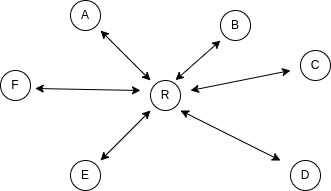
\includegraphics[width=\textwidth]{images/Centralized.png}
    \caption{Cellular network topology}
    \label{fig:centralized}
  \end{subfigure}
  \hfill
  \begin{subfigure}[b]{0.48\textwidth}
    \centering
    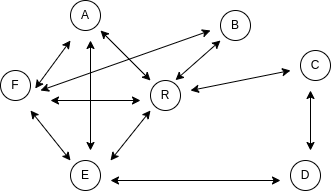
\includegraphics[width=\textwidth]{images/Decentralized.png}
    \caption{Ad-hoc network topology}
    \label{fig:decentralized}
  \end{subfigure}
  \caption{Network topology models for geodistributed agents. Edges represent communication links (bidirectional for simplicity).}
  \label{fig:nettopology}
\end{figure}

One can also imagine hybrid models, such as an ad-hoc arrangement of
localized cells. In general, one expects more centralized topologies to
be simpler for application developers to reason about, but to require
more physical infrastructure and support. On the other hand, the ad-hoc
model is more fault resistant, but more complicated to implement and
potentially offering fewer assurancess about performance. In either
case, higher-level applications such as shared memory abstractions
should be tuned for the networking environment. It would be even better
if this tuning can take place dynamically, with applications
reconfiguring manually or automatically to the particulars of the
operating environment. This requires examining the relationship between
the application and networking layers, rather than treating them as
separate blackboxes.

\hypertarget{delay-tolerant-networking}{%
  \subsection{Delay-tolerant networking}\label{delay-tolerant-networking}}

\hypertarget{ad-hoc-dtns}{%
  \subsection{Ad-hoc DTNs}\label{ad-hoc-dtns}}

An interesting possibility is for the \emph{network} to automatically
configure itself to the quality-of-service needs of the application. For
example, a client that receives a lot of requests may be marked as a
preferred client and given higher-priority access to the network. If UAV
vehicles can be used to route messages by acting as mobile transmission
base stations, one can imagine selecting a flight pattern based on
networking needs. For example, if the communication between two
firefighting teams is obstructed by a geographical feature, a UAV could
be dispatched to provide overhead communication support. Such an
arrangement could greatly blur the line between the networking and
application layers.

\hypertarget{software-defined-networking}{%
  \subsection{Software-defined
    networking}\label{software-defined-networking}}

\hypertarget{verification-of-networking-protocols}{%
  \subsection{Verification of networking
    protocols}\label{verification-of-networking-protocols}}

\newpage

\hypertarget{continuous-consistency}{%
  \section{Continuous Consistency}\label{continuous-consistency}}

\label{sec:continuous-consistency}

Strong consistency is a discrete proposition: an application provides
strong consistency or it does not. For many real-world applications, it
evidently makes sense to work with data that is consistent up to some
\(\epsilon \in \mathbb{R}^{\geq 0}\). Thus, we shift from thinking about
consistency as an all-or-nothing condition, towards consistency as a
bound on inconsistency.

The definition of \(\epsilon\) evidently requires a more or less
application-specific notion of divergence between replicas of a shared
data object. Take, say, an application for disseminating the most
up-to-date visualization of the location of a fire front. It may be
acceptable if this information appears 5 minutes out of date to a
client, but unacceptable if it is 30 minutes out of date. That is, we
could measure consistency with respect to \emph{time}. One should expect
the exact tolerance for \(\epsilon\) will be depend very much on the
client, among other things. For example, firefighters who are very close
to a fire have a lower tolerance for stale information than a central
client keeping only a birds-eye view of several fire fronts
simultaneously.

Now suppose many disaster-response agencies coordinate with to update
and propagate information about the availability of resources. A client
may want to lookup the number of vehicles of a certain type that are
available to be dispatched within a certain geographic range. We may
stipulate that the value read by a client should always be \(4\) of the
actual number, i.e.~we could measure inconsistency with respect to some
numerical value.

In the last example, the reader may wonder we should tolerate a client
to read a value that is incorrect by 4, when clearly it is better to be
incorrect by 0. Intuitively, the practical benefit of tolerating weaker
values is to tolerate a greater level of imperfection in network
communications. For example, suppose Alice and Bob are individually
authorized to dispatch vehicles from a shared pool. In the event that
they cannot share a message.

Or, would could ask that the the value is a conservative estimate,
possibly lower but not higher than the actual amount. In these examples,
we measure inconsistency in terms of a numerical value.

As a third example,

By varying \(\epsilon\), one can imagine consistency as a continuous
spectrum. In light of the CAP theorem, we should likewise expect that
applications with weaker consistency requirements (high \(\epsilon\))
should provide higher availability, all other things being equal.

Yu and Vahdat explored the CAP tradeoff from this perspective in a
series of papers \cite{2000tact,2000tactalgorithms,10.5555/1251229.1251250,DBLP:conf/icdcs/YuV01,2002tact}
propose a theory of \emph{conits}, a logical unit of data subject to
their three metrics for measuring consistency. By controlling the
threshold of acceptable inconsistency of each conit as a continuous
quantity, applications can exercise precise control the tradeoff between
consistency and performance, trading one for the other in a gradual
fashion.

They built a prototype toolkit called TACT, which allows applications to
specify precisely their desired levels of consistency for each conit. An
interesting aspect of this work is that consistency can be tuned
\emph{dynamically}. This is desirable because one does not know a priori
how much consistency or availability is acceptable.

The biggest question one must answer is the competing goals of
generality and practicality. Generality means providing a general notion
of measuring \(\epsilon\), while practicality means enforcing
consistency in a way that can exploit weakened consistency requirements
to offer better overall performance.

\begin{itemize}
\item
  The tradeoff of CAP is a continuous spectrum between linearizability
  and high-availability. More importantly, it can be tuned in real time.
\item
  TACT captures neither CAP-consistency (i.e.~neither atomic nor
  sequential consistency) nor CAP-availability (read and write requests
  may be delayed indefinitely if the system is unable to enforce
  consistency requirements because of network issues).
\end{itemize}

\hypertarget{causal-consistency-1}{%
  \subsection{Causal consistency}\label{causal-consistency-1}}

Causal consistency is that each clients is consistent with a total order
that contains the happened-before relation. It does not put a bound on
divergence between replicas. Violations of causal consistency can
present clients with deeply counterintuitive behavior.

\begin{itemize}
  \tightlist
\item
  In a group messaing application, Alice posts a message and Bob
  replies. On Charlie's device, Bob's reply appears before Alice's
  original message.
\item
  Alice sees a deposit for \$100 made to her bank account and, because
  of this, decides to withdraw \$50. When she refreshes the page, the
  deposit is gone and her account is overdrawn by \(50\). A little while
  later, she refreshes the page and the deposit reappears, but a penalty
  has been assessed for overdrawing her account.
\end{itemize}

In these scenarios, one agent takes an action \emph{in response to} an
event, but other processes observe these causally-related events taking
place in the opposite order. In the first example, Charlie is able to
observe a response to a message he does not see, which does not make
sense to him. In the second example, Alice's observation at one instance
causes her to take an action, but at a later point the cause for her
actions appears to have occurred after her response to it. Both of these
scenarios already violate atomic and sequential consistency because
those models enforce a system-wide total order of events. Happily, they
are also ruled out by causally consistent systems. The advantage of the
causal consistency model is that it rules out this behavior without
sacrificing system availability, as shown below.

Causal consistency enforces a global total order on events that are
\emph{causally related}. Here, causal relationships are estimated very
conservatively: two events are potentially causally if there is some way
that the outcome of one could have influenced another.

\begin{figure}
  \center
  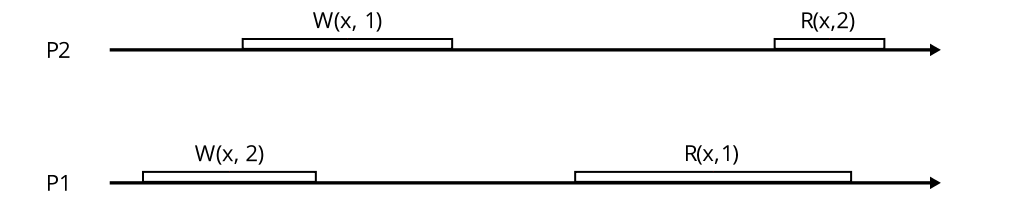
\includegraphics[scale=0.4]{images/causal1.png}
  \caption{A causally consistent, non-sequentially-consistent execution}
\end{figure}

\begin{lemma}
  Sequential consistency implies causal consistency.
\end{lemma}
\begin{proof}
  This is immediate from the definitions. Sequential consistency
  requires all processes to observe the same total order of events,
  where this total order must respect program order. Causal consistency
  only requires processes to agree on events that are potentially
  causally related. Program order is a subset of causal order, so any
  sequential executions also respects causal order.
\end{proof}

However, causal consistency is not nearly as strong as sequential
consistency, as processes do not need to agree on the order of events
with no causal relation between them. This weakness is evident in the
fact that the CAP theorem does not rule out highly available systems
that maintain causal consistency even during network partitions.

\begin{lemma}
  A causally consistent system need not be unavailabile during partitions.
\end{lemma}
\begin{proof}

  Suppose $P_1$ and $P_2$ maintain replicas of a key-value store, as
  before, and suppose they are separated by a partition. The strategy is
  simple: each process immediately handles read requests by reading from
  its local replica, and handles write requests by applying the update
  to its local replica. It is easy to see this leads to causally
  consistent histories. Intuitively, the fact that no information flows
  between the processes also means the events of each process are not
  related by causality, so causality is not violated.  \end{proof}

Note that in this scenario, a client's requests are always routed to the
same processor. If a client's requests can be routed to any node, causal
consistency cannot be maintained without losing availability. One
sometimes says that causal consistency is ``sticky available'' because
clients must stick to the same processor during partitions.

The fact that causal consistency can be maintained during partitions
suggests it is too weak. Indeed, there are no guarantees about the
difference in values for \(x\) and \(y\) across the two replicas.

\hypertarget{tact-system-model}{%
  \subsection{TACT system model}\label{tact-system-model}}

As in Section \ref{sec:background}, we assume a distributed set of
processes collaborate to maintain local replicas of a shared data object
such as a database. Processes accept read and write requests from
clients to update items, and they communicate with each other to ensure
to ensure that all replicas remain consistent.

However, access to the data store is mediated by a middleware library,
which sits between the local copy of the replica and the client. At a
high level, TACT will allow an operation to take place if it does not
violate user-specific consistency bounds. If allowing an operation to
proceed would violate consistency constraints, the operation blocks
until TACT synchronizes with one or more other remote replicas. The
operation remains blocked until TACT ensures that executing it would not
violate consistency requirements.

\[\textrm{Consistency} = \langle \textrm{Numerical error, \textrm{Order error}, \textrm{Staleness}} \rangle.\]

Processes forward accesses to TACT, which handles commiting them to the
store. TACT may not immediately process the request---instead it may
need to coordinate with other processes to enforce consistency. When
write requests are processed (i.e.~when a response is sent to the
originating client), they are only commited in a \emph{tenative} state.
Tentative writes eventually become fully committed at some point in the
future, but when they are commited, they may be reordered. After
fullying committing, writes are in a total order known to all processes.

\begin{figure}[h]
  \center
  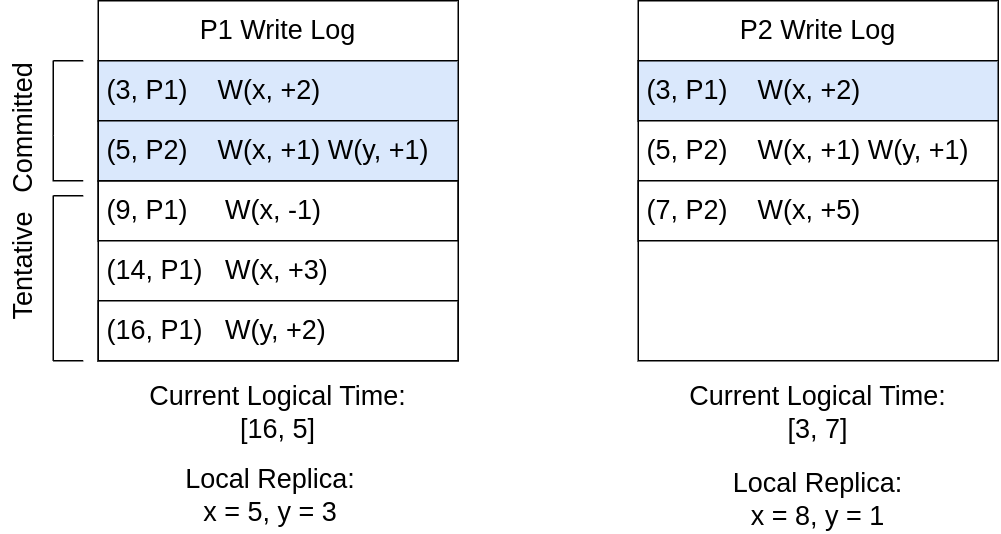
\includegraphics[scale=0.4]{images/TACT Logs.png}
  \caption{Snapshot of two local replicas using TACT}
  \label{fig:tact_logs}
\end{figure}

A write access \(W\) can separately quantify its \emph{numerical weight}
and \emph{order weight} on conit \(F\). Application programmers have
multiple forms of control:

Consistency is enforced by the application by setting bounds on the
consistency of read accesses. The TACT framework then enforces these
consistency levels.

\hypertarget{measuring-consistency-on-conits}{%
  \subsection{Measuring consistency on
    conits}\label{measuring-consistency-on-conits}}

\hypertarget{numerical-consistency}{%
  \paragraph{Numerical consistency}\label{numerical-consistency}}

\hypertarget{order-consistency}{%
  \paragraph{Order consistency}\label{order-consistency}}

When the number of tentative (uncommitted) writes is high, TACT executes
a write commitment algorithm. This is a \emph{pull-based} approach which
pulls information from other processes in order to advance \(P_i\)'s
vector clock, raising the watermark and hence allowing \(P_i\) to commit
some of its writes.

\hypertarget{real-time-consistency}{%
  \paragraph{Real time consistency}\label{real-time-consistency}}

\hypertarget{enforcing-inconsistency-bounds}{%
  \subsection{Enforcing inconsistency
    bounds}\label{enforcing-inconsistency-bounds}}

\hypertarget{numerical-consistency-1}{%
  \paragraph{Numerical consistency}\label{numerical-consistency-1}}

We describe split-weight AE. Yu and Vahdat also describe two other
schemes for bounding numerical error. One, compound AE, bounds absolute
error trading space for communication overhead. In their simulations,
they found minimal benefits to this tradeoff in general. It is possible
that for specific applications the savings are worth it. They also
consider a scheme, Relative NE, which bounds the relative error.

\hypertarget{order-consistency-1}{%
  \paragraph{Order consistency}\label{order-consistency-1}}

\hypertarget{real-time-consistency-1}{%
  \paragraph{Real time consistency}\label{real-time-consistency-1}}

\hypertarget{future-work}{%
  \subsection{Future work}\label{future-work}}

\hypertarget{data-fusion}{%
  \section{Data Fusion}\label{data-fusion}}

\cite{1999:lucien-datafusion}

\label{sec:data-fusion}

Strong consistency models provide the abstraction of an idealized global
truth. In the case of conits, the numerical, commit-order, and real-time
errors are measured with respect to an idealized global state of the
database. This state may not exist on any one replica, but it is the
state each replica would converge to if it were to see all remaining
unseen updates.

We consider distributed applications that receive data from many
different sources, such as from a sensor network (broadly defined). It
will often be the case that some sources of data should be expected to
agree with each other, but they may not. A typical scenario, we want to
integrate these data into a larger model of some kind. Essentially take
a poll, and attempt to synthesize a global picture that agrees as much
as possible with the data reported from the sensor network.

Here, we need a consistency model to measure how successful our attempts
are to synthesize a global image. And to tell us how much our sensors
agree. Ideally, we could use this system to diagnose disagreements
between sensors, identifying sensors that appear to be malfunctioning,
or to detect abberations that necessitate a response.

\hypertarget{fusion-centers}{%
  \subsection{Fusion centers}\label{fusion-centers}}

To be written.

\hypertarget{sheaf-theory}{%
  \subsection{Sheaf theory}\label{sheaf-theory}}

\hypertarget{introduction-to-presheaves}{%
  \subsubsection{Introduction to
    presheaves}\label{introduction-to-presheaves}}

\begin{definition}
  A \emph{partially order-indexed family of sets} is a family of sets indexed by a partially-ordered set,
  such that orders between the indices correspond to functions between the sets.
\end{definition}

We can also set \((P, \leq)\) \emph{acts on} the set
\(\{S_i\}_{i \in I}\).

\begin{definition}
  A \emph{semiautomaton} is a monoid paired with a set.
\end{definition}

This is also called a \emph{monoid action} on the set.

\begin{definition}
  A copresheaf is a *category acting on a family of sets*.
\end{definition}

\begin{definition}
  A presheaf is a *category acting covariantly on a family of sets*.
\end{definition}

\hypertarget{introduction-to-sheaves}{%
  \subsubsection{Introduction to sheaves}\label{introduction-to-sheaves}}

To be written.

\hypertarget{the-consistency-radius}{%
  \subsubsection{The consistency radius}\label{the-consistency-radius}}

To be written.

\hypertarget{conclusion}{%
  \section{Conclusion}\label{conclusion}}

\label{sec:conclusion}

To be written.

\section*{Bibliography}\label{bibliography}
\addcontentsline{toc}{section}{Bibliography}

\bibliographystyle{abbrv}
\bibliography{bibliography}


\begin{figure}[p]
  \begin{subfigure}[a]{1\textwidth} \center
    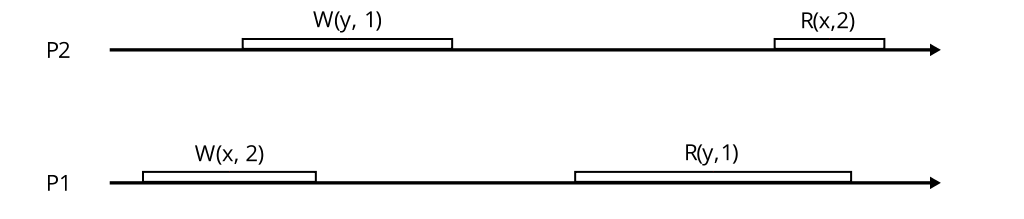
\includegraphics[scale=0.4]{images/linear1.png} \caption{A
      linearizable execution. Any choice of linearization works here.}
    \label{fig:linear_example11} \end{subfigure}
  \begin{subfigure}[b]{1\textwidth} \center
    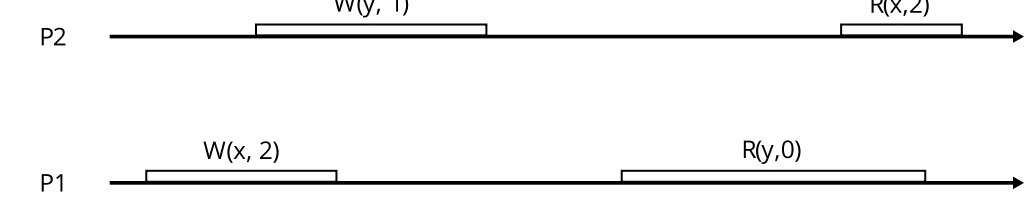
\includegraphics[scale=0.4]{images/nonlinear0.png} \caption{A
      non-linearizable execution. The request to read $y$ returns a
      stale value. } \label{fig:linear_example12} \end{subfigure}
  \caption{A linearizable and non-linearizable execution.}
  \label{fig:linear_example1} \end{figure}

\begin{figure}[p]
  \begin{subfigure}[a]{1\textwidth}
    \center
    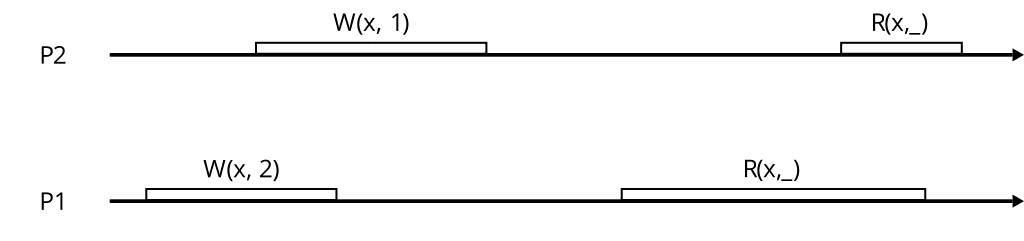
\includegraphics[scale=0.4]{images/linearTemplate.png}
    \caption{An execution with read responses left unspecified.}
    \label{fig:nonlinear}
  \end{subfigure}
  \begin{subfigure}[b]{1\textwidth}
    \center
    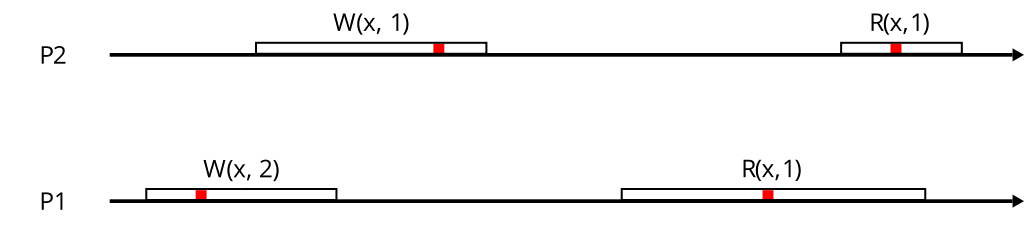
\includegraphics[scale=0.4]{images/linear3.png}
    \caption{A linearizable execution for which both reads return $1$.}
  \end{subfigure}
  \begin{subfigure}[c]{1\textwidth}
    \center
    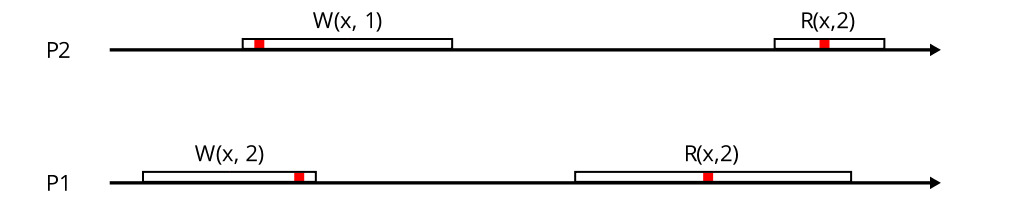
\includegraphics[scale=0.4]{images/linear2.png}
    \caption{A linearizable execution for which both reads return $2$.}
  \end{subfigure}
  \caption{Two linearizable executions of the same underlying events that return different responses. Possible linearization points are shown in red.}
  \label{fig:linearization}
\end{figure}

\begin{figure}[p]
  \begin{subfigure}[a]{1\textwidth}
    \center
    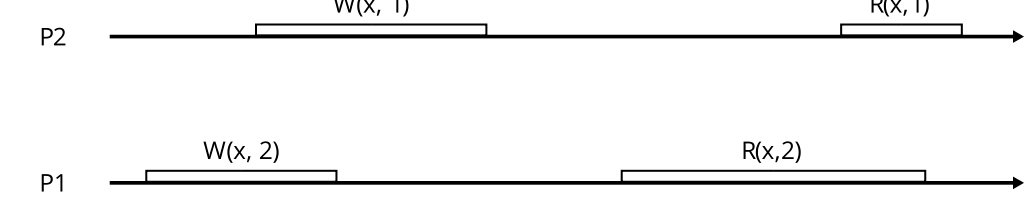
\includegraphics[scale=0.4]{images/nonlinear1.png}
    \caption{A nonlinearizable execution with the read access returning disagreeing values. We will see later (Figure \ref{fig:sequential}) that this execution is still sequentially consistent. }
    \label{fig:nonlinear1}
  \end{subfigure}
  \begin{subfigure}[b]{1\textwidth}
    \center
    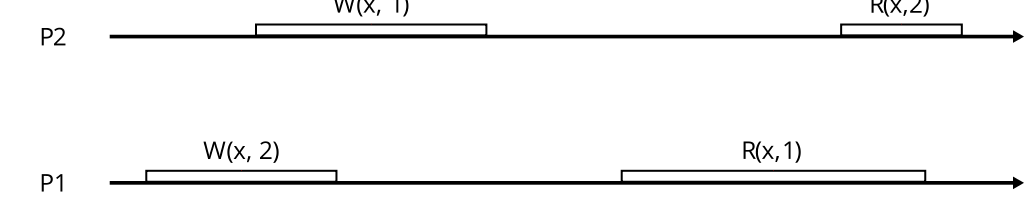
\includegraphics[scale=0.4]{images/nonlinear2.png}
    \caption{Another nonlinearizable execution with read access values swapped. This execution is not sequentially consistent.}
    \label{fig:nonlinear2}
  \end{subfigure}
  \caption{Two non-linearizable executions of the same events shown in Figure \ref{fig:linearization}.}
  \label{fig:nonlinearizable}
\end{figure}

\begin{figure}
  \begin{subfigure}[a]{1\textwidth}
    \center
    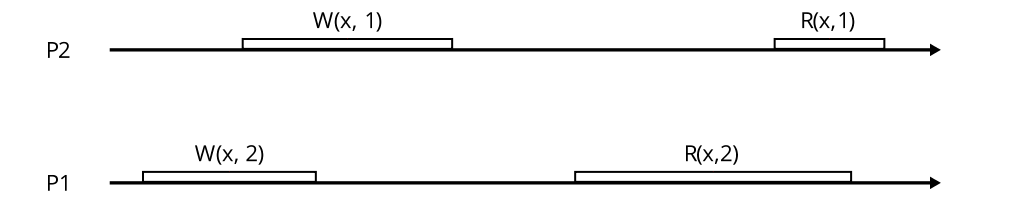
\includegraphics[scale=0.4]{images/sequential1.png}
    \caption{A non-linearizable, sequentially consistent execution.}
    \label{fig:sequential1}
  \end{subfigure}
  \begin{subfigure}[b]{1\textwidth}
    \center
    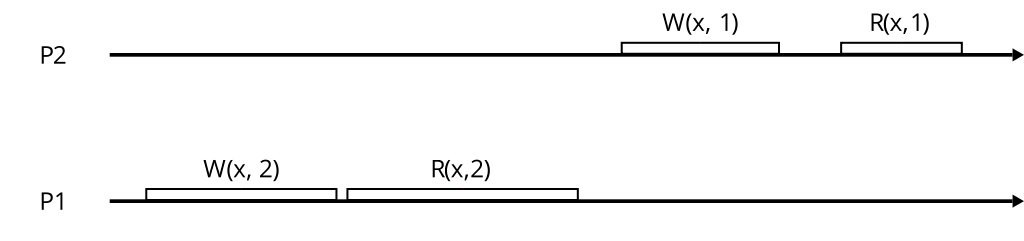
\includegraphics[scale=0.4]{images/sequential2.png}
    \caption{An equivalent interleaving of \ref{fig:sequential1}.}
    \label{fig:interleaving1}
  \end{subfigure}
  \caption{A sequentially consistent execution and a possible interleaving.}
  \label{fig:sequential}
\end{figure}

\begin{figure}
  \begin{subfigure}[a]{1\textwidth}
    \center
    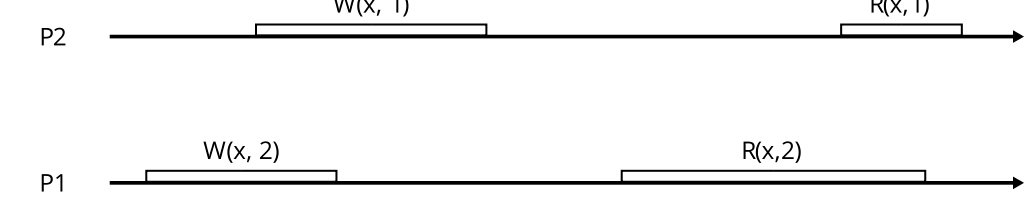
\includegraphics[scale=0.4]{images/nonsequential1.png}
    \caption{A non-sequentially consistent execution.}
    \label{fig:nonsequential1}
  \end{subfigure}
  \begin{subfigure}[b]{1\textwidth}
    \center
    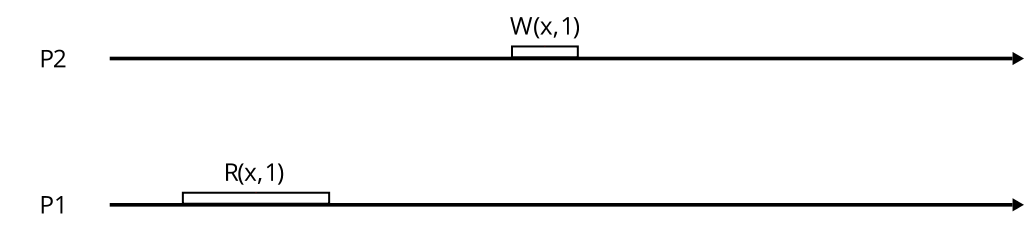
\includegraphics[scale=0.4]{images/nonsequential_x.png}
    \caption{The sequentially consistent history of $x$.}
    \label{fig:sequentialx}
  \end{subfigure}
  \begin{subfigure}[b]{1\textwidth}
    \center
    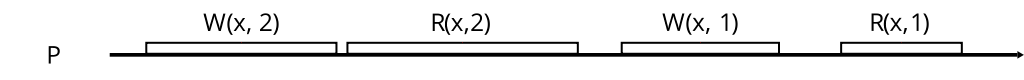
\includegraphics[scale=0.4]{images/nonsequential_y.png}
    \caption{The sequentially consistent history of $y$.}
    \label{fig:sequentialy}
  \end{subfigure}
  \caption{A non-sequentially consistent execution with sequentially-consistent executions at each variable.}
  \label{fig:nonsequential}
\end{figure}


\end{document}
